\documentclass[12pt]{extarticle}

%%%% paramètres généraux et commande prédéfinies
\input{_parametres}
% \modeCorrection % correction (décommenté)

%%%% pour l'en-tête
\renewcommand{\annee}{2023-2024}
\renewcommand{\etablissement}{Lycée Jean Moulin}

%% Priorités :


%%%% doc
\begin{document}
  %%%% Commun
  % \includepdf[pages=26]{commun/papier_millimetre.pdf}
  % \newpage
\pasDePagination
\begin{center}
  \image{0.3}{images/chimie/protocoles/dissolution0001}
  \image{0.3}{images/chimie/protocoles/dissolution0006}
  \image{0.3}{images/chimie/protocoles/dissolution0003} \\[2pt]
  \image{0.3}{images/chimie/protocoles/dissolution0005}
  \image{0.3}{images/chimie/protocoles/dissolution0004}
  \image{0.3}{images/chimie/protocoles/dissolution0002}
  \\[16pt]
  \image{0.3}{images/chimie/protocoles/dissolution0001}
  \image{0.3}{images/chimie/protocoles/dissolution0006}
  \image{0.3}{images/chimie/protocoles/dissolution0003} \\[2pt]
  \image{0.3}{images/chimie/protocoles/dissolution0005}
  \image{0.3}{images/chimie/protocoles/dissolution0004}
  \image{0.3}{images/chimie/protocoles/dissolution0002}
\end{center}
  % \pasDePagination

\titre{Règles de sécurités en chimie}

\large

\sousTitre{Les 4 règles de bases :}
\begin{enumerate}
  \item Ne pas manger.
  \item Ne pas boire.
  \item Ne pas sentir.
  \item Ne pas toucher.
\end{enumerate}
Sauf indication du contraire.


\sousTitre{Pictogrammes de danger :}
\newcommand{\imagePicto}[1]{\image{0.18}{images/securite/picto_#1}}
\begin{center}
  \imagePicto{ronge}
  \imagePicto{pollue}
  \imagePicto{toxique}
  \imagePicto{sante}
  \imagePicto{tue} \\ 
  \imagePicto{flambe}
  \imagePicto{flamber}
  \imagePicto{explose}
  \imagePicto{pression}
\end{center}


\titre{Port de la blouse, des gants et des lunettes de protection obligatoire en travaux pratiques !}
\begin{center}
  \image{0.6}{images/securite/picto_gant_blouse_lunette}
\end{center}

\normalsize
\textbf{Signature élève :}
  % \newpage
\pasDePagination

%%%%
\titre{Règles de vie en classe}

\large

\begin{listePoints}
  \item \important{Le règlement intérieur s'applique en classe.}
  \item Pas de prise de parole sans autorisation.
  \item Pas de déplacement sans autorisation.
  \item Téléphone silencieux et rangés.
  \item Pas de retards acceptés passé 5 minutes.
  \item Les documents du chapitre en cours doivent \important{tous} être amenés.
\end{listePoints}

\begin{center}
  \important{Objectif : avoir un cadre de travail serein et agréable.}
\end{center}

\vspace*{-0.2cm}
\ligne

%%%
\titre{Règles d'évaluation}


\important{Les devoirs sur table}

\begin{listePoints}
  \item 1 ou 2 devoirs sur table par trimestre.
  \item \important{Date et sujet communiqués une ou deux semaines en avance.}
  \item Coefficient 3.
\end{listePoints}


\important{Les travaux pratiques}

\begin{listePoints}
  \item Évaluation des compte-rendus.
  \item Évaluation de certaines activités réalisées en classe.
  \item Évaluation de la maîtrise des gestes expérimentaux.
  \item Coefficient 2.
\end{listePoints}


\important{La progression}

\begin{listePoints}
  \item Évaluation variable (classeur, DM, interrogation).
  \item Coefficient 0,5 ou 1.
\end{listePoints}

% \bigskip
% \normalsize
% \important{Exemple :} Avec $8/20$, $9/20$, $11/20$ en devoir sur table et $10/20$ en travaux pratiques, un ou une élève assidue ($> 15/20$ en progression), s'assure une moyenne supérieure à $10/20$ (contre $9,\!5/10$ sans la progression).

% \bigskip
% \normalsize
% \important{Signature élève :}
  % %%%%
\titre{Progression annuelle première ST2S}

\phantom{\important{premStssChim}}\\
\refstepcounter{section} \important{\premStssChim} \\
\refstepcounter{section} \important{\premStssVisi} \\ 
\refstepcounter{section} \important{\premStssRedo} \\ 
\refstepcounter{section} \important{\premStssLumi} \\ 
\refstepcounter{section} \important{\premStssStru} \\ 
\refstepcounter{section} \important{\premStssBiom} \\
\refstepcounter{section} \important{\premStssRout} \\
\refstepcounter{section} \important{\premStssAlim} \\
\refstepcounter{section} \important{\premStssElec} \\
\refstepcounter{section} \important{\premStssPres} \\
\refstepcounter{section} \important{\premStssSono} \\


%%%
\titre{Progression annuelle terminale ST2S}

\setcounter{section}{0}
\phantom{\important{premStssChim}}\\
\refstepcounter{section} \important{\termStssOrga} \\
\refstepcounter{section} \important{\termStssAlim} \\
\refstepcounter{section} \important{\termStssImag} \\
\refstepcounter{section} \important{\termStssBiom} \\
\refstepcounter{section} \important{\termStssMedi} \\
\refstepcounter{section} \important{\termStssEnvi} \\
\refstepcounter{section} \important{\termStssDosa} \\
\refstepcounter{section} \important{\termStssRout} \\
\refstepcounter{section} \important{\termStssCosm} \\


  %%%% Matériel TP
  % \begin{boiteMateriel}{\Large Fiche de préparation de TP}
\end{boiteMateriel}

\begin{center}
  \begin{tblr}{
      colspec = {|l X[l] |l X[l] |}, hlines, width = \linewidth,
    }
    \textbf{Date :}     & 15/11/23 et 16/11/23 
    & \textbf{Niveau :} & Terminale ST2S \\
    %
    \textbf{Matière :}  & Physique-Chimie
    & \textbf{Salle :}  & A108 (mercredi) et A104 (jeudi) \\
    %
    \textbf{Heure :}    & 12h40-14h40
    & \textbf{Prof :}   & Alexandre Jedrecy \\
    %
    \textbf{Titre :} & Fraicheur d'un lait
    & & \\
  \end{tblr}
\end{center}

\begin{boiteMateriel}{Matériel élève}
  \separationBlocs{
    \textbf{Effectif :} 15
  }{
    \flecheLongue \textbf{5 groupes} de 3 élèves
  }

  \begin{listePoints}
    \item Burette et son support
    \item Agitateur magnétique
    \item barreau aimanté
    \item Erlen-meyer 250 mL
    \item Bécher 100 mL
  \end{listePoints}
\end{boiteMateriel}

\begin{boiteMateriel}{À préparer}
  \begin{listePoints}
    \item \qty{500}{\ml} de solution d'hydroxyde de sodium $c = \qty{0,05}{\mol\per\litre}$.
    \item Bouteille de lait > \qty{0,5}{\litre}.
    \item Phénolphtaléine (ou bleu de bromothymol idéalement, mais j'ai l'impression qu'il n'y en a plus...)
  \end{listePoints}
\end{boiteMateriel}


  %% Divers
  % \qrcode{https://nosgestesclimat.fr/tutoriel}
  % \begin{center}    
  \chemfig{
    NH_2 !\glycine N(-[-3] H) !\alanine N(-[-3] H) !\glycine OH
  }
  \bigskip  
  
  \chemfig{
    NH_2 !\glycine N(-[-3] H) !\alanine N(-[-3] H) !\glycine OH
  }
\end{center}
\vspace*{-2.95cm}
  
\begin{tikzpicture}
  \draw (0, 0);
  \draw[couleurPrim, line width = 1.5mm]
    (6.65, 0) -- (8.15, 0) -- (8.15, 2.75) -- (6.65, 2.75) -- cycle;
  \draw[couleurPrim, line width = 1.5mm]
    (9.5, 0) -- (11, 0) -- (11, 2.75) -- (9.5, 2.75) -- cycle;
\end{tikzpicture}
\bigskip

\begin{center}
  \chemname{\chemfig{
    NH_2 !\alanine OH
  }}{Alanine}
  \qq{}
  \chemname{\chemfig{
    NH_2 !\glycine OH
  }}{Glycine}
  \bigskip
  
  \chemfig{
    !\testosterone
  }
  \bigskip

  \chemfig{
    C_4 H_7 N_3 O
  }

  \begin{equation*}
    \isotope{125}{53}{I} + \isotope{0}{-1}{e^{-}} 
    \reaction 
    \isotope{125}{52}{Te} + \gamma 
  \end{equation*}
  \bigskip
  
  \begin{equation*}
    \textbf{RAC} = \dfrac{c_m \text{(albumine)}}{c_m \text{(créatinine)}}
  \end{equation*}
  \bigskip
\end{center}

  
  %%%% Terminale ST2S
  % %%%%
\teteTermStssMeth

%%%% titre
\numeroActivite{1}
\vspace*{-36pt}
\titreActivite{L'analyse dimensionnelle}

\begin{objectifs}
  \item Comprendre la notion d'équation homogène
  \item Réaliser de l'analyse dimensionnelle
\end{objectifs}

\begin{contexte}
  En physique, une relation est correcte si elle est \important{homogène :} les membres de droites et de gauche de l'égalité doivent être exprimé avec la même \important{unité.}

  \problematique{Comment vérifier que les deux côté d'une égalité sont bien exprimés dans la même unité ?}
\end{contexte}

%%%%
\vspace*{-8pt}
\titreSection{Les puissances négatives}
\vspace*{-8pt}

%%
\begin{doc}{Puissance négative}{doc:A2_puissance_negative}
  Une puissance indique combien de fois on répète une multiplication.
  ($3^3 = 3\times 3 \times 3 = 27$)

  Une puissance \important{négative} correspond à une division par une puissance.
  $\left(5^{-2} = \dfrac{1}{5^2}\right)$

  \begin{encart}
    On a les mêmes règles de calculs avec les unités.
    $\left(\dfrac{1}{\unit{\s}} = \unit{\per\s}, \quad
    \unit{\per\m\cubed} = \dfrac{1}{\unit{\m\cubed}}\right)$
  \end{encart}
\end{doc}

\begin{doc}{Multiplication d'unité}{doc:A2_multiplication_unite}
  \begin{encart}
    Quand on multiplie deux unités entre elles, la multiplication est indiquée par un point médian $\cdot$
    
    \exemple $\unit{\kilo\watt\hour} = \unit{\kilo\watt}\times\unit{\hour}$
  \end{encart}
\end{doc}


\begin{multicols}{2}
  \numeroQuestion Relier les valeurs égales entre elles.
  \begin{center}
    \begin{tblr}{ colspec = {c c X[1,c] c c}, width = 0.5\linewidth }
      $4^{-2}$  & \pointCyan & & \pointCyan & $\dfrac{1}{10}$ \\
      $25^{-1}$ & \pointCyan & & \pointCyan & \num{0,04} \\
      $10^{-1}$   & \pointCyan & & \pointCyan & $\dfrac{1}{4^2}$ \\
                &            & & \pointCyan & \num{0,10}
    \end{tblr}
  \end{center}
  
  \numeroQuestion Relier les unités égales entre elles.
  \begin{center}
    \begin{tblr}{ colspec = {c c X[1,c] c c}, width = 0.5\linewidth }
      \unit{\m\per\second}                 & \pointCyan & & \pointCyan & $\dfrac{\unit{\kg}}{\unit{\cubic\m}}$ \\
      \unit{\kg\per\cubic\m}               & \pointCyan & & \pointCyan & \unit{\cubic\m\per\s} \\
      $\dfrac{\unit{\cubic\m}}{\unit{\s}}$ & \pointCyan & & \pointCyan & $\dfrac{\unit{m}}{\unit{s}}$ \\
      \unit{\m/\s}                         & \pointCyan & & &
    \end{tblr}
  \end{center}
\end{multicols}


%%%%
\titreSection{Opérations et unités}

\sisetup{unit-color = couleurQuat}

\begin{doc}{Calcul d'une unité}{doc:A2_produits_quotient}
  \begin{encart}  
    Si une grandeur est le produits de plusieurs grandeurs, son unité est le produit des unités de ces grandeurs.

    De même si une grandeur est le quotient de plusieurs grandeurs.
  \end{encart}

  \exemple Une vitesse $v = \dfrac{d (\unit{\m})}{\Delta t (\unit{s})}$ s'exprime en $\dfrac{\unit{\m}}{\unit{s}}$, c'est-à-dire en \unit{\m/\s} ou \unit{\m\per\s}.

  \begin{encart}
    Pour additionner ou soustraire deux grandeurs, elles doivent être de même unités.

    Le résultat du calcul s'exprime dans les même unités que les grandeurs additionnées ou soustraites.
  \end{encart}

  \exemple La masse d'une molécule d'eau $\eau$ est la somme de la masse des atomes qui la compose 
  $m_{\eau} = 2\times m_H + m_O 
  = 2\times\qty{1,7e-27}{\kg} + \qty{26,7e-27}{\kg}
  = \qty{30,1e-27}{\kg}$
\end{doc}

\numeroQuestion Sans calcul, déterminer l'unité du membre de gauche de l'égalité. \\

\begin{tblr}{
    colspec = {X[2,l] | X[2,c] }, width = \linewidth,
    row{1} = {couleurPrim!20}, hlines
  }
  Grandeur & Unité \\
  Longueur $L = L_1 (\unit{\m}) + L_2 (\unit{m}) + L_3 (\unit{\m})$ \vphantom{$\dfrac{1}{2}$} & \\
  Fréquence $f = \dfrac{1}{T (\unit{\s})}$ & \\
  Concentration massique $c = \dfrac{m (\unit{\kg})}{V (\unit{\m\cubed})}$ & \\
  Intensité du courant $I = \dfrac{R_1 (\unit{\ohm})}{R_1 (\unit{\ohm}) + R_2 (\unit{\ohm})} \times I_1 (\unit{\ampere})$
\end{tblr}


%%%%
\titreSection{Homogénéité}

\begin{doc}{Relation homogène}{doc:A2_homogene}
  \begin{encart}  
    Une relation entre grandeurs ne peut être correcte que si elle est \important{homogène.}
    C'est-à-dire si les membres à droite et à gauche de l'égalité s'exprime avec les \important{même unités.}
  \end{encart}
  
  Toute égalité entre deux grandeurs qui ne peuvent pas s'exprimer avec les mêmes unités est donc forcément \important{fausse.}
  On dit \important{qu'elle n'est pas homogène.}
  Vérifier l'homogénéité d'une équation c'est faire de \important{l'analyse dimensionnelle.}
\end{doc}

\numeroQuestion
Calculer les unités des grandeurs des deux côtés de l'égalité des relations suivantes.
Barrer les relations qui \textbf{ne sont pas homogènes.}
\begin{alignat*}{2}
  v &= \dfrac{f}{d} 
  &\hspace{5cm}
  F &= G\times\dfrac{m_1 \times m_2}{d^2} \\
  %
  m &= m_1 \times m_2
  &\hspace{5cm}
  v &= f \times d \\
  %
  m &= c_m \times V
  &\hspace{5cm}
  V_0 &= \dfrac{c_{m,1}}{c_{m,0}} V_1
\end{alignat*}

\textbf{Données :} unités des différentes grandeurs 

\begin{center}
  \begin{tblr}{ row{1} = {couleurPrim!20}, colspec = {c|c}, hlines }
    Grandeur & Unité \\
    $f$ & \unit{\per\s} (ou \unit{\hertz}) \\
    $d$ & \unit{\m} \\
    $m$ & \unit{\kg} \\
  \end{tblr}
  ~
  \begin{tblr}{ row{1} = {couleurPrim!20}, colspec = {c|c}, hlines }
    Grandeur & Unité \\
    $F$ & \unit{\kg\m\per\s\squared} (ou \unit{\newton}) \\
    $G$ & \unit{\m\cubed \per\kg \per\s\squared} \\
    $V$ & \unit{\litre} \\
  \end{tblr}
  ~
  \begin{tblr}{ row{1} = {couleurPrim!20}, colspec = {c|c}, hlines }
    Grandeur & Unité \\
    $c_m$ & \unit{\kg\per\litre} \\
    $t$ & \unit{\s} \\
    $v$ & \unit{\m\per\s}
  \end{tblr}
\end{center}
  %% Méthodologie
  % %%%%
\teteTermStssOrga

%%%% titre
\numeroActivite{1}
\vspace*{-30pt}
\titreActivite{Représenter des molécules organiques}

%%%% objectifs
\begin{objectifs}
  \item Rappeler les règles de formation des molécules et la valence d'un atome
  \item Rappeler les différentes représentations des molécules organiques
\end{objectifs}

\begin{contexte}
  Les atomes de carbones peuvent se lier entre eux pour former des \textbf{chaînes carbonées}, de formes et de tailles variées.
  Ces chaînes carbonées, une fois liée à des atomes d'hydrogène, d'oxygène ou d'azote, forment des \textbf{molécules organiques}.
  Il existe ainsi des millions de molécules organiques différentes.

  \problematique{
    Comment peut-on représenter ces molécules ?
  }
\end{contexte}


%%
\vspace*{-8pt}
\titreSection{La valence}
\vspace*{-8pt}

%%
\begin{doc}{Éléments composant un corps humain}{doc:element_corps_humain}
  Le corps humain est composé majoritairement de 4 éléments chimiques :
  \vspace*{-4pt}
  \begin{multicols}{2}
  \begin{listePoints}
    \item l'oxygène   \chemfig{O} (\qty{65}{\percent} en masse),
    \item le carbone  \chemfig{C} (\qty{18}{\percent}),
    \item l'hydrogène \chemfig{H} (\qty{10}{\percent})
    \item et l'azote  \chemfig{N} (\qty{3}{\percent}).
  \end{listePoints}
  \end{multicols}
  
  \begin{encart}
    \important{Numéro atomique :} il correspond au nombre de protons d'un atome et est noté $Z$ : \isotope{A}{Z}{X} (\hspace{-8pt}\exemple \isotope{12}{6}{C})
    Par neutralité de l'atome, c'est aussi son nombre d'électrons.
  \end{encart}
\end{doc}

%%
\begin{doc}{Liaison moléculaire}{doc:liaison_molecule}
  %
  À partir du numéro atomique d'un atome, on peut déterminer sa structure électronique en couche (1, 2 ou 3) et sous-couche (s ou p), puis sa \important{valence} (mono, bi, tri ou tétravalent).
  %
  \begin{encart}
    Pour former des molécules, les atomes partagent les électrons de leur couche externe pour former des \important{liaison covalentes}.
    Chaque liaison covalente apporte 1 électron à l'atome.
    La \important{valence} est le nombre de liaisons formées par l'atome.
  \end{encart}
  %
  \begin{encart}
    La couche 1 contient au maximum \textbf{2 électrons} et les couches 2 et 3 contiennent jusqu'à \textbf{8 électrons}.

    Les atomes cherchent à remplir leur couche externe : c'est la règle du \important{duet} (couche 1) ou de \important{l'octet} (couche 2 ou 3).
  \end{encart}
  %
  Pour connaître la valence d'un atome, il suffit donc de compter combien d'électrons il lui manque pour remplir sa couche externe.

  \exemple \isotope{}{6}{C} : $1^2 2^4$,
  il lui manque \textbf{4} électrons pour compléter sa couche externe et respecter la règle de \textbf{l'octet.}
  Il fera donc \textbf{4} liaisons, il est \textbf{tétravalent}.
\end{doc}


%% questions
\question{%
  Indiquer la configuration électronique de l'oxygène \isotope{}{8}{C}, combien d'électrons il lui manque pour respecter la règle du duet ou de l'octet, le nombre de liaisons ainsi formées et sa valence.
}{%
  \isotope{}{8}{C} : $1^2; 2^6$,
  il lui manque 2 électrons pour respecter la règle de l'octet, il formera donc 2 liaisons. Il est bivalent.
}{2}

%
\question{%
  Même question pour l'azote \isotope{}{7}{N} et l'hydrogène \isotope{}{1}{H}.
}{%
}{4}


%%
\begin{doc}{Liaisons multiples}{doc:liaisons_multiples}
  %
  \begin{encart}
    Pour compléter leur couche externe et respecter la règle de l'octet, deux atomes peuvent se lier en formant 2 ou 3 liaisons covalentes.
    
    On dit qu'il y a une \texteTrou{liaison double}{0.3} ou une \texteTrou{liaison triple}{0.3}
  \end{encart}
\end{doc}

%
\numeroQuestion
Indiquer si les liaisons sont simples, triples ou doubles sur les molécules suivantes :
\begin{equation}
  \chemfig{
    N~N
  } \qq{}
  \chemfig{
    O=C=O
  } \qq{}
  \chemfig{
    H-C~N
  }
\end{equation}


%%
\titreSection{Les représentations des molécules}

%%
\titreSousSection{La formule brute}

\begin{doc}{Formule brute}{doc:formule_brute}
  \begin{encart}
    Elle indique le nombre de chaque élément présent dans la molécule.
  \end{encart}
  Elle permet de calculer facilement les \important{masses molaires} et de vérifier si deux molécules sont \important{isomères}.

  \begin{encart}
    Deux molécules sont \important{isomères} si elles ont la même formule brute, mais un agencement des atomes différents.
  \end{encart}

  \exemple Le butane \chemfig{C_4 H_{10}}. L'éthanol \chemfig{C_2 H_6 O}. 
\end{doc}

L'oxybenzone est une molécule utilisée pour protéger des UVA et B issu du soleil.
Sa formule brute est \chemfig{C_14 H_12 O_3}.

\question{%
  Indiquer le nombre d'élément d'hydrogène, d'oxygène et de carbone dans la molécule d'oxybenzone.
}{%
  Il y a 12 hydrogènes, 3 oxygènes et 14 carbones.
}{1}


La taurine est un acide aminé produit naturellement dans le corps humain.
Sa représentation avec un modèle moléculaire est présentée à gauche.

\question{%
  Donner la formule brute de la taurine.
}{%
  \chemfig{C_2 H_7 O_3 N}
}{1}


%%
\titreSousSection{La formule développée}

\begin{doc}{Formule développée}
  \label{doc:formule_developpee}
  %
  Elle représente tous les éléments chimiques et toutes les liaisons dans le même plan.

  \exemples
  \begin{equation*}
    \chemfig{
      H 
      - C (-[3] O (-[5] H)) (-[9] H)
      - C (-[3] H) (-[9] H)
      - H
    }
    %éthanol
    \qq{}
    \chemfig{
      Cl
      - C (-[3] H) (-[9] H)
      - Si (-[3] H) (-[9] H)
      - H
    }
    %chlorométhylsilane
    \qq{}
    \chemfig{
      *6 (C (-[7] O (-[5] H))
        - C (-[9] H)
        = C (-[-1] H)
        - C (-[1] N 
          (-[3] H) (-[-1] C 
            (=[1] O) (-[10] C (-[0] H) (-[6] H) (-[9] H))
          )
        )
        = C (-[3] H)
        - C (-[5] H) (=[9,0.75])
      )
    }
    %paracétamol
  \end{equation*}
\end{doc}

%%
\titreSousSection{La formule semi-développée}

\begin{doc}{Formule semi-développée}
  \label{doc:formule_semi_developpee}

  Comme la formule développée, elle représente tous les éléments chimiques, mais elle ne détaille pas les liaisons des éléments \textbf{hydrogènes}.

  \exemples
  \begin{equation*}
    \chemfig{CH_2 (-[3] OH) - CH_3}
    %éthanol
    \qq{}
    \chemfig{Cl - CH_2 - Si H_3}
    %chlorométhylsilane
    \qq{}
    \chemfig{
      *6 (C (-[7] HO)
        - CH
        = CH
        - C (-[1] NH
          (-[-1] C (=[1] O) (-[9] CH_3))
        )
        = CH
        - CH (=[9,0.75,2])
      )
    }
    %paracétamol
  \end{equation*}
\end{doc}


%%
\titreSousSection{La formule topologique}

\begin{doc}{Formule topologique}
  \label{doc:formule_topologique}

  Elle représente les liaisons \textbf{carbone-carbone \chemfig{C - C}} par des segments formant un angle de \qty{30}{\degree}.
  Les éléments \textbf{carbones} et \textbf{hydrogènes} qui sont attachés aux carbones \textbf{ne sont pas représentés}.
  Tous les autres éléments chimiques sont représentés normalement.

  \exemples
  \begin{equation*}
    \chemfig{HO -[1] -[11]}
    %éthanol
    \qq{}
    \chemfig{Cl-[1] -[11] Si H_3}
    %chlorométhylsilane
    \qq{}
    \chemfig{
      *6 ((-[7] HO)
        -=- (-[1] NH
          (-[-1] (=[1] O) (-[9]))
        )
        =-=
      )
    }
    %paracétamol
  \end{equation*}
\end{doc}

%
\question{%
 bla
}{%
 bla
}{2}

  % %%%%
\teteTermStssOrga

%%%% titre
\numeroActivite{2}
\vspace*{-34pt}
\titreActivite{Fonctions organiques et nomenclature}

%%%% objectifs
\begin{objectifs}
  \item Rappeler les 8 familles organiques à connaitre et la nomenclature associée.
\end{objectifs}


%%
\vspace*{-8pt}
\titreSection{Les fonctions organiques}

%%
\vspace*{-8pt}
\begin{doc}{Fonctions organiques}{doc:A2_fonction_organique}
  Certaines séquences d'éléments donnent des \important{propriétés} spécifiques aux molécules organiques que l’on classe en différentes familles ou fonctions organiques ou encore famille fonctionnelle.

  % \begin{importants}  
    En ST2S on étudie à 8 familles : \important{alcool, aldéhyde, cétone, acide carboxylique, ester, éther, amine et amide.}
  % \end{importants}
  \medskip

  \begin{tblr}{
    colspec = {c c c Q[t, wd=0.26\linewidth]}, hlines, vlines,
    column{2, 3} = {couleurSec-50}, row{1} = {couleurSec-100},
    cell{3}{1} = {r=2}{c}, rows = {m}, columns = {c}
  }
    Groupe caractéristique & Famille organique & Formule & Exemple \\
    %
    Hydroxyle & Alcool
    & \chemfig{R_1 - \textcolor{couleurQuat}{OH}} 
    & {\chemfig{-[1] -[-1] OH} \\[1pt] éthanol} \\
    %
    Carbonyle & \vAligne{-40pt} Cétone
    & \vAligne{-60pt} \chemfig{\textcolor{couleurQuat}{C} !\alkyleG !\cetoneCouleur R_2}
    & {\chemfig{-[1] !\carbonyle -[1]} \\[1pt] butan-2-one} \\
    %
    & Aldéhyde
    & \chemfig{\textcolor{couleurQuat}{C} !\alkyleG !\cetoneCouleur \textcolor{couleurQuat}{H}}
    & {\chemfig{O=[-3] -H} \\[1pt] méthanal } \\
    %
    Carboxyle & Acide carboxylique
    & \chemfig{\textcolor{couleurQuat}{C} !\alkyleG !\cetoneCouleur \textcolor{couleurQuat}{OH}}
    & {\chemfig{-[-1] -[1] !\carboxyle} \\[1pt] acide propanoïque} \\
    %
    \vAligne{-34pt} Ester & \vAligne{-34pt} Ester
    & \chemfig{R_1 -[1] \textcolor{couleurQuat}{C} !\cetoneCouleur \textcolor{couleurQuat}{O} -[1] R_2}
    & {\chemfig{-[1] -[-1] -[1] !\ester -[1] -[-1]} \\[1pt] butanoate d'éthyle} \\
    %
    Éther-oxyde & Éther
    & \chemfig{R_1 -[1,,,,couleurQuat] \textcolor{couleurQuat}{O} -[-1,,,,couleurQuat] R_2}
    & {\chemfig{-[-1] -[1] O -[-1] -[1]} \\[1pt] éthoxyéthane} \\
    %
    Amine & Amine
    & \chemfig{R_1 - \textcolor{couleurQuat}{NH_2}}
    & {\chemfig{-[1] -[-1] -[1] NH_2} \\[1pt] propan-1-amine} \\
    %
    Amide & Amide
    & \vAligne{-48pt} \chemfig{\textcolor{couleurQuat}{C} !\alkyleG !\cetoneCouleur \textcolor{couleurQuat}{N} (-[-3] R_3) - R_2}
    & {\chemfig{-[-1] -[1] !\amide H_2} \\[1pt] propanamide}
  \end{tblr}
  \smallskip

  $R_1,$ $R_2$ et $R_3$ sont des chaînes carbonées appelées \important{« radicaux alkyles ».}

  \begin{importants}
    Pour trouver les groupes caractéristiques d'une molécule, il faut repérer tous les éléments qui ne sont ni des carbones, ni des hydrogènes.
  \end{importants}
\end{doc}
% \begin{doc}{Fonctions organiques}{doc:A2_fonction_organique}
%   Certaines séquences d'éléments donnent des \important{propriétés} spécifiques aux molécules organiques que l’on classe en différentes familles : alcane, alcène, alcyne, alcool, aldéhyde, cétone, acide carboxylique, ester, éther, amine, amide, etc.

%   $R_1,$ $R_2$ et $R_3$ sont des chaînes carbonées appelées « radicaux alkyles ».
  
%   \begin{tblr}{
%     width = \linewidth,
%     colspec = {|c |c |c |Q[t, wd=0.3\linewidth]|}, hlines,
%     column{2} = {couleurPrim!20},
%     row{1} = {couleurPrim!10},
%     cell{3}{1} = {r=2}{c},
%     rows = {m}, columns = {c}
%   }
%     Groupe caractéristique & Famille fonctionnelle & Formule & Exemple \\
%     %
%     Hydroxyle & Alcool
%     & \chemfig{R_1 - \textcolor{couleurQuat}{OH}} 
%     & {\chemfig{-[1] -[-1] OH} \\[1pt] éthanol} \\
%     %
%     Carbonyle & Cétone
%     & \chemfig{\textcolor{couleurQuat}{C} !\alkyleG !\cetoneCouleur R_2}
%     & {\chemfig{-[1] !\carbonyle -[1]} \\[1pt] butan-2-one} \\
    
%     %
%     & Aldéhyde
%     & \chemfig{\textcolor{couleurQuat}{C} !\alkyleG !\cetoneCouleur \textcolor{couleurQuat}{H}}
%     & {\chemfig{!\carbonyle H} \\[1pt] méthanal ou formaldéhyde } \\
%     %
%     Carboxyle & Acide carboxylique
%     & \chemfig{\textcolor{couleurQuat}{C} !\alkyleG !\cetoneCouleur \textcolor{couleurQuat}{OH}}
%     & {\chemfig{-[-1] -[1] !\carboxyle} \\[1pt] acide propanoïque} \\
%     %
%     Ester & Ester
%     & \chemfig{R_1 -[1] \textcolor{couleurQuat}{C} !\cetoneCouleur \textcolor{couleurQuat}{O} -[1] R_2}
%     & {\chemfig{-[1] -[-1] -[1] !\ester -[1] -[-1]} \\[1pt] butanoate d'éthyle} \\
%     %
%     Éther-oxyde & Éther
%     & \chemfig{R_1 -[1,,,,couleurQuat] \textcolor{couleurQuat}{O} -[-1,,,,couleurQuat] R_2}
%     & {\chemfig{-[-1] -[1] O -[-1] -[1]} \\[1pt] éthoxyéthane} \\
%     %
%     Amine & Amine
%     & \chemfig{R_1 - \textcolor{couleurQuat}{NH_2}}
%     & {\chemfig{-[1] -[-1] -[1] NH_2} \\[1pt] propan-1-amine} \\
%     %
%     Amide & Amide
%     & \chemfig{\textcolor{couleurQuat}{C} !\alkyleG !\cetoneCouleur \textcolor{couleurQuat}{N} (-[-3] R_3) - R_2}
%     & {\chemfig{-[-1] -[1] !\amide H_2} \\[1pt] propanamide}
%   \end{tblr}
% \end{doc}


%%
\newpage
\vspace*{-24pt}
\titreSection{La nomenclature}

\begin{doc}{Principe de la nomenclature}{doc:A2_principe_nomenclature}
  \begin{importants}  
    La \important{nomenclature} est l'ensemble des règles établies pour nommer les molécules organiques.
  \end{importants}
   
  La nomenclature moderne repose sur deux principes :
  \begin{listePoints}
    \item décrire la \important{géométrie} de la molécule nommée ;
    \item indiquer les \important{fonction organiques} présentes dans la molécule.
  \end{listePoints}
\end{doc}

%%
\begin{doc}{Nommer une chaîne carbonée}{doc:A2_chaine_carbonee}
  Toute molécule organique possède au moins une chaîne carbonée.
  Pour nommer une chaîne carbonée, on va associer un \important{préfixe} avec un \important{suffixe.}
  Le suffixe dépend de la fonction organique, mais le préfixe est déterminé par le nombre de carbones qui composent la chaîne.
  \begin{importants}
  \begin{center}
    \begin{tblr}{
      columns = {c}, vlines, hlines,
      row{1} = {couleurPrim!20!white},
      column{1} = {couleurPrim!10}
    }
      Nombre de carbone \chemfig{C} 
      & 1 & 2 & 3 & 4 & 5 & 6 & 7 & 8\\
      Préfixe
      & meth- & éth- & prop- & but- & pent- & hex- & hept- & octa- \\
    \end{tblr}
  \end{center}  
  \end{importants}
\end{doc}

%%
\titreSousSection{Règles pour les alcanes, alcènes ou alcynes}

\begin{doc}{Les alcanes}{doc:A2_alcanes}
  \separationBlocs{
    \begin{importants}
      Une molécule d'alcane est un \important{hydrocarbure} composé de \important{liaisons simples.}
    \end{importants}
    Pour nommer un alcane, il faut déterminer la chaîne carbonée la plus longue qui compose la molécule. \\
    On écrit alors le préfixe lié à la longueur de la chaîne et on ajoute le suffixe « \important{-ane} ». \\
    Un alcane a toujours une formule brute de la forme \chemfig{ C_{n} H_{2(n + 1)} }.
  }{
    \vspace*{-22pt}
    \begin{importants}
      Un \important{hydrocarbure} est une molécule qui ne contient que des éléments carbones et hydrogènes.
    \end{importants}
    \begin{importants}
      Un hydrocarbure est \important{saturé} (en hydrogène) s'il ne comporte que des \important{liaisons carbone-carbone simples.} \\
      Si l'hydrocarbure comporte des \important{liaisons doubles} ou \important{triples,} on dit qu'il est \important{insaturé.}
    \end{importants}
  }
  
  \vspace*{4pt}
  \exemple \chemfig{H_3C - CH_2 - CH_3} trois carbones dans la chaîne, donc prop- $+$ -ane : propane.
\end{doc}

%%%% Question
\question{
  Nommer les molécules suivantes :
  \begin{equation*}  
    \chemfig{H_3C -CH_2 -CH_2 -CH_3} \qq{}
    \chemfig{-[1] -[-1] -[1] -[-1] -[1]} \qq{}
    \chemfig{H -C !\paireH -C !\saturationH}
  \end{equation*}
}{
  Butane, hexane et éthane.
}{2}


%%
\begin{doc}{Les alcènes}{doc:OA_2alcenes}
  \begin{importants}
    Les alcènes sont des hydrocarbures avec au moins une liaison double.
    Le suffixe « -ane », devient « \important{-ène} ».
    On indique le (ou les) numéro de la liaison double avant le suffixe, de sorte que \important{le numéro soit le plus petit possible.}
  \end{importants}
  \exemple \chemfig{H_3C- CH_2 - CH = CH -CH_3} cinq carbones dans la chaîne (pent-) et la liaison double se trouve en position 3 ou 2 (si on compte depuis la droite).
  Donc pent $+$ 2 $+$ ène : pent-2-ène.
\end{doc}

%%
\begin{doc}{les alcynes}{doc:A2_alcynes}
  \begin{importants}
    Les alcynes sont des hydrocarbures avec au moins une liaison triple.
    Le suffixe « -ane », devient « \important{-yne} ».
    On indique le (ou les) numéro de la liaison triple avant le suffixe, de sorte que \important{le numéro soit le plus petit possible,} comme pour les alcènes.
  \end{importants}
  \exemple \chemfig{-[1] ~[-1]} : trois carbones dans la chaîne (prop-) et la liaison triple se trouve en position 1.
  Donc prop-1-yne ou propyne (le 1 est implicite).
\end{doc}


%%
\titreSousSection{Règles pour les ramifications}
\vspace*{-8pt}

\begin{doc}{Ramification à la chaîne principale}{doc:A2_ramification}
  \begin{importants}  
    Une \important{ramification} est un substituant qui remplace un hydrogène sur la chaîne principale.
  \end{importants}
  Si le substituant est un \important{alkyle} (un hydrocarbure), son nom prend le suffixe « \important{-yl} ».

  \exemple* \chemfig{CH_3 -[6]} : méthyl, \chemfig{CH_2 (-[6]) -CH_3} éthyl.
\end{doc}

\begin{doc}{Nommer une ramification}{doc:A2_nom_ramification}
  \begin{importants}
  Pour nommer une molécule contenant des ramifications, il faut :
  \begin{listePoints}
    \item trouver la \important{plus longue chaîne carbonée} pour déterminer son nom.
    \item \important{Numéroter} la chaîne carbonée afin que la ramification ait le numéro le plus \important{petit possible,} comme pour les alcènes ou les alcynes.
    \item Placer le \important{numéro} et le \important{nom} de l'alkyle avant le nom de la chaîne.
    \item S'il y a plusieurs ramifications, leurs noms sont placés par ordre alphabétique.
  \end{listePoints}
  \end{importants}
\end{doc}

\question{
  Nommer les molécules suivantes :
  \begin{equation*}  
    \chemfig{H_3C- CH (-[3]CH_3) - CH (-[-3]CH_2 -CH_3) -CH_3} \qq{}
    \chemfig{H_3C- CH_2 -C (-[-3]CH_3) (-[3]CH_3) -CH_2 -CH_2 - CH_3}
  \end{equation*}
}{
  Pour la molécule 1 : la chaîne principale a 4 atomes, donc -butane.
  Deux ramifications sont en position 2 (avec un méthyl) et 3 (avec un éthyl).
  Donc le nom de cette molécule est 3-éthyl-2-méthyl-butane.

  Pour la molécule 2 : la chaîne principale a 5 atomes, donc -pentane.
  Deux ramifications méthyl sont en position 2 et 3.
  Donc le nom de cette molécul est 2,3-méthyl-pentane.
}{2}

%%
\newpage
\vspace*{-28pt}

\question{
  Donner la formule semi-développée du 4-méthyl-octane.
}{}{2}

\titreSousSection{Règles pour les groupes caractéristiques}

\begin{doc}{Groupes caractéristiques}{doc:A2_nom_groupe_carac}
  \vspace*{-4pt}
  \begin{wrapfigure}[5]{r}{0.58\linewidth}
    \vspace*{-30pt}
    \centering
    \begin{tikzpicture}[help lines/.style={thin,draw=black!50}]
      % chaine principale et carbone fonctionnel
      \large
      \node[draw] at (3,3) { \chemfig{
        H_3C-CH-CH_2 -\textcolor{couleurSec}{\textsf{\textbf{C}}} H-CH_3
        }
      };
      \draw (5, 2.25) node[right] {\textbf{chaîne principale}};
      \draw[couleurSec] (3.7, 3.7) node[right] {\textbf{carbone fonctionnel}};
      % Ramification
      \draw[very thick, couleurPrim] (1.51, 2.79) -- (1.51, 2.29);
      \draw[couleurPrim] (2.5, 1.3)  node[left] {\textbf{ramification}};
      \node[draw, couleurPrim] at (1.8, 2) { \chemfig{CH_3} };
      % Alcool
      \draw[very thick, violet] (4.11, 2.79) -- (4.11, 2.29);
      \draw[violet] (3.6, 1.3)  node[right] {\textbf{groupe caractéristique}};
      \node[draw, violet] at (4.28, 2){ \chemfig{OH_{}} };
    \end{tikzpicture}
  \end{wrapfigure}
  %
  Pour nommer les molécules contenant des groupes caractéristiques, on utilise les règles décrites dans le tableau ci-dessous, en respectant la priorité des fonctions organiques.
  
  \begin{importants}
    Le \important{carbone fonctionnel} désigne le carbone contenant la fonction de la molécule.
  \end{importants}
  
  Pour les cétones, alcools et amines, le numéro est celui du \important{carbone fonctionnel,} comme pour les ramifications il \important{doit être le plus petit possible.}
  
  ($R_1$) et ($R_2$) représentent les noms des chaînes carbonées auxquels les groupes caractéristiques sont attachées. 

  \vspace*{2pt}
  \begin{center}
  \begin{tblr}{
    width = \linewidth,
    colspec = {|c |c |c |Q[wd=0.4\linewidth] |}, hlines,
    column{2} = {couleurPrim!20},
    row{1} = {couleurPrim!10},
    rows = {m}, columns = {c}
  }
    Priorité & Famille fonctionnelle & Formule & Nom si prioritaire \\
    %
    1 & Acide carboxylique
    & \chemfig{\textcolor{couleurQuat}{C} !\alkyleG !\cetoneCouleur \textcolor{couleurQuat}{OH}}
    & acide ($R_1$)-oïque \\
    %
    2 & Ester
    & \chemfig{\textcolor{couleurQuat}{C} !\alkyleG !\cetoneCouleur \textcolor{couleurQuat}{O} -[1] R_2}
    & ($R_1$)-oate de ($R_2$)-yle \\
    %
    3 & Amide
    & \chemfig{\textcolor{couleurQuat}{C} !\alkyleG !\cetoneCouleur \textcolor{couleurQuat}{N} H_2}
    & ($R_1$)-amide \\
    %
    4 & Aldéhyde
    & \chemfig{\textcolor{couleurQuat}{C} !\alkyleG !\cetoneCouleur \textcolor{couleurQuat}{H}}
    & ($R_1$)-al \\
    %
    5 & Cétone
    & \chemfig{\textcolor{couleurQuat}{C} !\alkyleG !\cetoneCouleur R_2}
    & ($R_1$)-(numéro)-one \\
    %
    6 & Alcool
    & \chemfig{R_1 - \textcolor{couleurQuat}{OH}}
    & ($R_1$)-(numéro)-ol \\
    %
    7 & Amine & \chemfig{R_1 - \textcolor{couleurQuat}{NH_2}}
    & ($R_1$)-(numéro)-amine \\
    %
    8 & Éther
    & \chemfig{R_1 -[1,,,,couleurQuat] \textcolor{couleurQuat}{O} -[-1,,,,couleurQuat] R_2}
    & ($R_1$)-oxy-($R_2$) \\
  \end{tblr}
  \end{center}

  \vspace*{2pt}
  \begin{importants}
    \attention Pour ces 8 familles organiques, vous devez savoir :
    \begin{listePoints}
      \item les noms de chacune des familles et leur groupes fonctionnels ;
      \item les reconnaître dans une molécule si on vous en donne une représentation.
    \end{listePoints}
  \end{importants}
\end{doc}

% \question{
%   Nommer la molécule du document~\ref{doc:A2_nom_groupe_carac}.
% }{
%   4-méthyl-pent-2-ol
% }{1}
  %% Sécurité routière
  % \input{stssTerminale/securite_routiere/routA1_explosion}
  % \input{stssTerminale/securite_routiere/routA2_airbag}
  % %%%%
\teteTermStssRout

%%%% titre
\numeroActivite{3}
\nomPrenomClasse
\titreActivite{Principe de fonctionnement d'un alcootest}

\begin{tableauCompetences}
  REA & Mettre en \oe{}uvre les étapes d’une démarche & & & \\
  VAL & Confronter un modèle à des résultats expérimentaux & & & \\
\end{tableauCompetences}


%%%% objectifs
\begin{objectifs}
  \item Comprendre le principe d'un alcootest
  \item Revoir les réaction d'oxydoréduction
\end{objectifs}


%%%% docs
\begin{doc}{Principe de l'alcootest}{doc:A3_alcootest}
  L'alcootest est constitué d'un tube en verre dans lequel on fait circuler l'air préalablement expiré dans un ballon en plastique de 1 litre.
  
  L'air expiré traverse une zone constituée de grains jaune-orangé de dichromate de potassium.

  Si l'haleine contient de l'alcool, le solide jaune-orangé devient vert.

  Un repère situé à peu près au premier tiers de la zone de détection indique la limite à ne pas dépasser.

  \centering
  \image{1}{images/photos/alcootest}
\end{doc}

%%
\begin{doc}{Dichromate de potassium}{doc:A3_dichromate}
  Le dichromate de potassium \chemfig{K_2 Cr_2 O_7} est un solide ionique constitué de cations potassium \chemfig{K^+} incolores et d'anions dichromate responsables de la couleur jaune-orangé.
  
  Le dichromate est un oxydant et les ions \chemfig{K^+} n'interviennent pas : ils sont spectateurs.

  L'anion dichromate est très toxique, cancérigène et nuit à l'environnement.
  \begin{center}
    \image{0.1}{images/securite/picto_flambe}
    \image{0.1}{images/securite/picto_ronge}
    \image{0.1}{images/securite/picto_tue}
    \image{0.1}{images/securite/picto_pollue}
    \image{0.1}{images/securite/picto_sante}
  \end{center}
\end{doc}

\begin{doc}{Réaction d'oxydo-réduction dans un alcootest}{doc:A3_reaction_chim_alcootest}
  L'alcootest exploite une réaction chimique d'oxydoréduction.

  L'éthanol \chemfig{CH_3CH_2OH} contenu dans l'air expiré par une personne alcoolisée constitue le réducteur destiné à être oxydé en acide éthanoïque \chemfig{CH_3COOH} par l'ion dichromate contenu dans le tube.
  \smallskip

  \begin{tblr}{
    hlines, column{1} = {couleurPrim!20},
    colspec = {|l |X[c] |X[c] |}
  }
    Couple Ox/Red & \chemfig{Cr_2 O_7^{2-}}/\chemfig{Cr^{3+}} & \chemfig{C_2H_4O_2}/\chemfig{C_2H_6O} \\ 
    Couleurs & orange/vert & incolore/incolore \\
    %
    Demi-équation &
    {\chemfig{Cr_2 O_7^{2-}} 14\chemfig{H^+} + 6\chemfig{e^{–}} \\ = 2 \chemfig{Cr^{3+}} + 7 \chemfig{H_2O}} &
    {\chemfig{C_2H_4O_2} + 4\chemfig{H^+} + 4\chemfig{e^{–}} \\ = \chemfig{C_2H_6O} + \chemfig{H_2O}}
  \end{tblr}
\end{doc}

\begin{doc}{Démarche pour établir l'équation d'une réaction redox}{doc:A3}
  Pour établir l'équation d'une réaction d'oxydoréduction il faut
  \begin{listePoints}
    \item identifier les deux réactifs $Ox_1$ et $Red_2$.
    \item Écrire, l'une sous l'autre, les deux demi-équations en mettant les réactifs à gauche.
    \item Ajuster les coefficients des deux demi-équations pour obtenir le même nombre d'électrons.
    \item \og Additionner \fg\; les deux demi-équations.
    \item Supprimer les spectateurs éventuels.
    \item Vérifier que les charges et les éléments sont conservés.
  \end{listePoints}
\end{doc}

%%%%
\question{
  Établir l’équation de la réaction d’oxydoréduction sous la forme : $Ox_1 + Red_2 \reaction Red_1 + Ox_2$.
}{}{10}

\question{
  Interpréter les changements de couleurs observés lorsque l’alcootest est positif.
}{
}{4}
  %% Sécurité alimentaire
  % %%%%
\teteTermStssAlim

%%%% titre
\numeroActivite{1}
\titreActivite{Conservation d'huiles végétales}


%%%% objectifs
\begin{objectifs}
  \item Revoir ce qu'est un triglycéride
  \item Connaître les facteurs responsables de la dégradation d'une huile
\end{objectifs}

\begin{contexte}
  Les vergetures sont des petites stries pouvant apparaître sur la peau, particulièrement au moment de la grossesse. 
  Pour les prévenir, des massages à l’huile sont recommandés afin de nourrir la peau en profondeur et d’en conserver l’élasticité.
  
  \problematique{
    Comment conserver les huiles végétales utilisées ?
  }
\end{contexte}


%%%% docs
\begin{doc}{Les huiles végétales}{doc:A1_huiles_vegetales}
  \begin{encart}
    Une huile végétale est composée de \textbf{triesters de glycérol} et \textbf{d'acides gras} \important{saturés} ou \important{insaturés.}
  \end{encart}
  
  \begin{wrapfigure}{r}{0.22\linewidth}
    \centering
    \chemfig{OH -[-1] -[1] (-[3] OH) -[-1] -[1] OH} \\[4pt]
    {\small Glycérol}
  \end{wrapfigure}
  
  Par exemple, l'huile de coco est composée majoritairement de triesters \textbf{d'acide laurique} et \textbf{d'acide myristique}, et en quantité plus faible, d'autres acides tels que \textbf{l'acide oléique.}
  L'huile d'amande douce est composée en grande majorité de triesters \textbf{acides oléique} et \textbf{linoléique}.
  Comme elle rancit facilement, contrairement à l'huile de coco, il est nécessaire de l'acheter en petite quantité.
  
  \begin{center}
    Modèle moléculaires de quelques acides gras :
  \end{center}
  \vspace*{-24pt}
  \begin{multicols}{2}
    \centering
    \image{1}{images/organique/acide_laurique} \\
    {\small Acide laurique}
    
    \image{1}{images/organique/acide_oleique} \\
    {\small Acide oléique}
    
    \image{1}{images/organique/acide_mystirique} \\
    {\small Acide myristique}
    
    \image{1}{images/organique/acide_linoleique} \\
    {\small Acide linoléique}
  \end{multicols}
\end{doc}

\question{
  Préciser l'autre nom des triesters de glycérol et d'acides gras.
}{}{1}

\question{
  À partir des modèles moléculaires des acides gras représentés dans le document~\ref{doc:A1_huiles_vegetales}, justifier le nom d'acide donné à ces espèces.
}{}{2}

\question{
  Classer les acides gras du document~\ref{doc:A1_huiles_vegetales} en acide gras saturés et insaturés. Justifier.
}{}{4}


%%
\begin{doc}{Dégradation des huiles végétales}{doc:A1_degradation_huiles}
  Si les acides gras contenus dans une huile se dégradent, l’huile perd une partie de ses propriétés, change de couleur et développe une odeur de rance.
  \begin{encart}  
    \important{L’oxydation} est le principal phénomène à l’origine de cette dégradation.
  \end{encart}
  Le rancissement ne s'observe qu'avec des huiles contenant des graisses insaturées, car l'oxydation se fait au niveau des doubles liaisons carbone-carbone.
  \begin{encart}  
    Certains facteurs accélèrent cette oxydation comme l’exposition au dioxygène de l’air, à des température élevée, à la lumière (UV), etc.
  \end{encart}
  \begin{encart}
    Au contraire certains facteur ralentissent cette oxydation, comme \texteTrouLignes[1]{des température faibles, l'obscurité et l'absence de dioxygène, etc.}
  \end{encart}
\end{doc}


%%%%
\question{
  Expliquer la différence de comportement d'une huile d'amande et d'une huile de coco face au rancissement.
}{}{3}

\begin{doc}{Emballage d'une huile}{doc:A1_emballage}  
  L'emballage contenant un flacon d'huile d'amande douce mentionne \og Précaution de stockage : Conserver à l’abri de la chaleur et de la lumière \fg.
\end{doc}

\question{
  Justifier ces recommandations de stockage.
}{}{3}

\question{
  Justifier alors que le flacon en verre soit de couleur brune.
}{}{2}

\begin{doc}{Indice d’iode d’une huile végétale}{doc:A1_indice_iode}
  \important{L'indice d'iode $I_\text{iode}$} d'une huile est la masse de diiode \chemfig{I_2}, exprimée en gramme, se fixant sur les doubles liaisons des acides gras contenus dans \qty{100}{g} d’huile.
  
  L'indice d'iode d'un acide gras saturé est donc nul.
  On modélise la réaction du diiode \chemfig{I_2} sur un acide gras insaturé possédant une seule double liaison par l’équation :
  \begin{center}
    \chemfig{R_1- CH= CH- R_2} + \chemfig{I_2} \reaction \chemfig{R_1- CHI- CHI- R_2}
  \end{center}

  \begin{encart}
    L'indice d'iode permet de déterminer le degré d'insaturation d'un acide gras.
  \end{encart}
\end{doc}

\begin{doc}{Indices d'iodes de l'huile de coco et d'amande}{doc:A1_iode_huiles}
  L'indice d'iode d'une huile de coco est compris entre \num{6} et \qty{11}{\g} de diiode \chemfig{I_2} pour \qty{100}{\g} d'huile,
  alors que celui d'une huile d'amande douce est compris entre \num{92} et \qty{109}{\g} pour \qty{100}{\g} d'huile.
\end{doc}

\question{
  Justifier qualitativement cette différence entre les deux huiles.
}{}{2}

\question{
  En utilisant le document~\ref{doc:A1_indice_iode}, déterminer la quantité de matière de diiode \chemfig{I_2} qui peut réagir avec une mole d'acide linoléique.
}{}{2}

\question{
  Une quantité de matière $n = \qty{0,010}{\mole}$ d'acide linoléique réagit
  avec une masse $m = \qty{5,1}{\g}$ de diiode \chemfig{I_2}.
  Calculer la quantité de matière de diiode et vérifier qu'on retrouve bien le nombre de doubles liaisons que contient une molécule d’acide linoléique.
  
  \textbf{Données :} M(\chemfig{I_2}) = \qty{254,0}{\g\per\mole}
}{
}{4}


\question{
  Une quantité de matière $n = \qty{0,020}{\mole}$ d'acide $\alpha$-linolénique réagit avec une masse $m = \qty{15,2}{\g}$ de diiode \chemfig{I_2}.
  Calculer le nombre de double liaisons que contient une molécule d'acide $\alpha$-linolénique.
}{

}{4}

\newpage
\textit{Pour les plus rapides}

\question{
  Donner les formules brutes des acide laurique, myristique, oléique et linoléique.
}{}{4}

\question{
  Donner la formule topologique des acides laurique, myristique, oléique et linoléique.
}{}{8}
  % %%%%
\teteTermStssAlim

%%%% titre
\numeroActivite{2}
\titreActivite{Hydrolyse des triglycérides}


%%%% objectifs
\begin{objectifs}
  \item Connaître la réaction modélisant l'hydrolyse d'un triglycérides
\end{objectifs}

\begin{contexte}
  Les triglycérides sont une source importante d'énergie pour notre organisme.
  La dégradation des acides gras constituants les triglycérides permet de produire de \important{l'adénosine triphosphate}, ou \important{ATP}, qui fournit l'énergie nécessaire aux réactions chimiques du métabolisme cellulaire.
  
  \problematique{
    Quelle réaction chimique permet de séparer les triglycéride en acide gras ?  
  }
\end{contexte}
\vspace*{4pt}

%%%% docs
\begin{doc}{Hydrolyse de l'oléine}{doc:A2_hydrolyse_oleine}
  \begin{encart}
    \important{L'hydrolyse} (du grec \og hydro \fg: eau et \og lysis \fg : briser) est une réaction chimique et enzymatique dans laquelle une liaison covalente est rompue par action d'une molécule d'eau.
  \end{encart}

  L'oléine est un triglycéride constituant \qty{80}{\percent} de l'huile d'olive.
  
  Au cours de son absorption par l’organisme, \textbf{l’oléine} est \important{hydrolysée} à l'aide de la lipase pour former de \textbf{l'acide
oléique} selon l'équation suivante :
  \begin{center}
    \begin{tblr}{colspec = {c c c}}
      \SetCell[r=4]{c, m} \chemfig[atom sep = 14pt]{!\trioleine} & 
      \SetCell[r=5]{c, m} \reaction & 
      \chemfig[atom sep = 14pt]{H!\oleique} \\
      %
      & & + \chemfig[atom sep = 14pt]{H!\oleique} \\
      & & + \chemfig[atom sep = 14pt]{H!\oleique} \\
      & & + \chemfig[atom sep = 16pt]{!\glycerol} \\
      + \texteTrou{3} \chemfig{H_2O} & & 
    \end{tblr}
  \end{center}
  La masse molaire de l'oléine est $M_\text{oléine} = \qty{884}{\g\per\mole}$.
\end{doc}

\numeroQuestion
Dans le document~\ref{doc:A2_hydrolyse_oleine}, entourer les groupes caractéristiques de la molécule d'oléine et d'une molécule d'acide oléique.

\question{
  Donner le nom des deux molécules formées au cours de la réaction d'hydrolyse.
}{}{2}


\newpage
\vspace*{-24pt}
\question{
  Préciser si l'acide oléique est un acide gras saturé ou insaturé. Justifier.
}{}{2}


L'organisme hydrolyse une masse d'oléine $m_\text{oléine} = \qty{8,84}{\g}$.

\question{
  La réaction est supposée totale. Calculer la quantité de matière d'eau $n_\text{eau}$ qui a été transformé au cours de la réaction.
}{}{5}

\question{
  Donner la quantité de matière d'acide oléique produite au cours de la réaction.
}{}{1}



%%
\begin{doc}{La palmitine}{doc:A2_hydrolyse_palmitine}
  La palmitine est un des triglycérides les plus présents chez les être vivants, animaux ou végétaux.
  \begin{center}
    \chemfig[atom sep = 18pt]{[:-60] !\tripalmitine} \\[8pt]
    Formule topologique de la palmitine
  \end{center}
\end{doc}


%%%%
\question{
  Indiquer si la palmitine est un triglycéride saturé ou insaturé. Justifier.
}{}{2}

\question{
  Donner la réaction d'hydrolyse de la palmitine.
}{}{7}

  % \input{stssTerminale/securite_alimentation/alimA3_brunissement_pomme}
  % \input{stssTerminale/securite_alimentation/alimA4_procedes_conservation}
  % \input{stssTerminale/securite_alimentation/alimTP1_lait_degre_dornic}
  % %%%%
\teteTermStssAlim

%%%% titre
\numeroActivite{5}
\titreActivite{Contrôle qualité d'un dessert à base de lait}


%%%% objectifs
\begin{objectifs}
  \item Comprendre le principe de la \important{D}ose \important{J}ournalière \important{A}dmissible (\important{DJA})
  et de la \important{D}ose \important{J}ournalière \important{T}olérable (\important{DJT}).
\end{objectifs}

\begin{contexte}
  Une inspectrice sanitaire contrôle un restaurant et réalise un prélèvement sur un dessert pour enfant.

  \problematique{
    Est-ce que ce dessert respecte les doses toxicologiques de référence ?
  }
\end{contexte}


%%%% docs
\begin{doc}{Dose Journalière Admissible (DJA) et Dose Journalière Tolérable (DJT)}{doc:A5_DJA_DJT}
  \begin{encart}
    Les \important{Doses Journalières} sont les quantités d'une substance, qu'une personne peut manger tous les jours de sa vie sans risques pour sa santé.
  \end{encart}  

  Les \important{Doses Journalières} sont estimées par des études scientifiques et exprimées en \unit{\mg} de substance par \unit{\kg} de masse corporelle, soit en \unit{\mg\per\kg}.

  \begin{encart}
    On distingue deux types de \important{Doses Journalières}
    \begin{listePoints}  
      \item \important{DJA :} pour les substances autorisées et ajoutées volontairement ;
      \item \important{DJT :} pour les contaminants présent involontairement (métaux lourds, radionucléides, composés organiques, etc.)
    \end{listePoints}
  \end{encart}
\end{doc}

\begin{doc}{Lait de vache cru}{doc:A5_lait_vache_cru}
  Le lait de vache cru est le lait issu de la traite des vaches.
  Le lait est constitué à \qty{87,5}{\percent} d'eau, de glucides, de protéines et de matières grasses.

  Le lait peut-être contaminé par des polluants comme la mélamine, ou infecté par des micro-organismes.
  Ces micro-organismes peuvent venir de l'environnement (terre, paille, mouche, déjection, camion-citerne, etc.) ou être présents sur la vache (infection des mamelles).

  Pour que les micro-organismes prolifèrent, il faut de l'humidité (de l'eau), de l'énergie (sous forme de chaleur), de la nourriture (contenue dans le lait) et en général du dioxygène.
\end{doc}

\begin{doc}{Techniques de conservation des aliments}{doc:A5_technique_conservation}
  Pour tuer les micro-organismes, on peut augmenter la température d'un aliment pendant une certaine durée, avant de refroidir l'aliment rapidement.

  \begin{center}
    \begin{tblr}{
      colspec = {|c |c |c |c |}, hlines,
      column{1} = { couleurPrim!10 },
      row{1,2} = { couleurPrim!20 },
      cell{1}{1} = {r=2}{c},
      cell{1}{2} = {r=2}{c},
      cell{1}{3} = {c=2}{c},
    }
      Technique & Pasteurisation & Stérilisation & \\
      %
      & & Appertisation & Upérisation (UHT) \\
      %
      Température &
      Entre \qty{65}{\degreeCelsius} et \qty{100}{\degreeCelsius} &
      Environ \qty{120}{\degreeCelsius} &
      Environ \qty{140}{\degreeCelsius} \\
      %
      Durée &
      Quelques dizaines de secondes &
      Quelques secondes &
      Quelques secondes \\
    \end{tblr}
  \end{center}
\end{doc}
  
\begin{doc}{Doses toxicologiques de références}{doc:A5_doses_references}
  \centering
  \begin{tblr}{
    colspec = {|c |c |c |}, hlines,
    row{1} = { couleurPrim!20 },
    row{2} = { couleurPrim!10 },
    cell{1}{1} = {c=2}{c},
  }
    \textbf{DJA (\unit{\mg\per\kg})} & & \textbf{DJT (\unit{\mg\per\kg})} \\
    %
    E102 & E122 & Mélamine \\
    %
    \num{7,5} & \num{4} & \num{0,5} \\
  \end{tblr}
\end{doc}

\separationBlocs{
  \begin{doc}{Gâteau à analyser}{doc:A5_gateau}
    \image{1}{images/photos/conservation/gateau_DJA_DJT}
  \end{doc}
}{
  \begin{doc}{Analyse du dessert}{doc:A5_analyse_dessert}
    \centering
    \phantom{b}\vspace*{-12pt}
    
    \begin{tableau}{|c |c |c |}
      E102 (jaune) & E122 (rouge) & Mélamine \\
      %
      \qty{150}{\mg} & \qty{50}{\mg} & \qty{4}{\pico\g}
    \end{tableau}
    
    \phantom{b}
  \end{doc}
}

\smallskip
\question{
  Indiquer les méthodes de conservations utilisé pour conserver le lait dans le gâteau à analyser.
  Identifier si les méthodes de conservations sont des procédés physiques ou chimiques.
}{}{5}

\question{
  Calculer les masses maximales de colorant jaune E102, de colorant rouge E122 et de mélamine qu'un-e enfant de \qty{20}{\kg} peut ingérer chaque jour.
}{}{6}

\question{
  Le dessert peut-il être servi sans danger dans le restaurant ?
  Justifier en répondant à la problématique posée dans le contexte.
}{}{6}
  %% Sécurité environnementale
  % \input{stssTerminale/securite_environnement/enviA1_proprietes_eau}
  % \input{stssTerminale/securite_environnement/enviA2_pollution_eau_potable}
  % \input{stssTerminale/securite_environnement/enviTP1_controle_qualite}
  % \input{stssTerminale/securite_environnement/enviTP2_composition_air}
  % \input{stssTerminale/securite_environnement/enviA3_gaz_parfait}
  % %%%%
\teteTermStssEnvi

%%%% titre
%\vspace*{-32pt}
\numeroActivite{4}
\titreActivite{Pollution de l'air et dérèglement climatique}
\vspace*{-8pt}


%%%% objectifs
\begin{objectifs}
  \item Connaître les trois principaux gaz à effet de serre : \chemfig{CO_2}, \chemfig{CH_4} et \chemfig{H_2O}.
  \item Comprendre le principe de « l'effet de serre ».
  \item Connaître les principales sources de pollutions et d'émission de gaz à effet de serre.
\end{objectifs}

\begin{contexte}
  Certaines activités humaines sont source de pollution pour l'air.
  Elles émettent des \important{polluants nocifs} pour la vie ou qui sont des \important{gaz à effet de serre}, responsable du \important{dérèglement climatique.}
  
  \problematique{ 
    Quelles sont les activités sources de pollution ?
    Quels sont les gaz à effets de serre et comment réchauffent-ils l'atmosphère ?
  }
\end{contexte}


%%%% Pollution & polluant
\begin{doc}{Les polluants de l'air et leurs conséquences sur la santé}{doc:A4_polluant_air}
  La pollution de l'air à des conséquences très négatives sur la santé et l'environnement.
  En France, la pollution de l'air représente
  \begin{listePoints}
    \item $\sim \num{40000}$ décès par an.
    \item $\sim 100$ milliards d'euros de dépense de santé par an 
  \end{listePoints}
  À titre de comparaison, le budget de toute l'éducation nationale représente 59 milliards d'euros par an. 
  Il y a \num{660 000} morts par an en France, donc $\num{40000}/\num{660000} = \qty{6}{\percent}$ des morts en France sont dus à la pollution de l'air : c'est l'équivalent d'une crise covid chaque année !

  \begin{encart}
    Il existe deux catégorie de polluants
    \begin{listePoints}
      \item les \important{polluants primaires} : monoxyde de carbone \chemfig{CO}, dioxyde de soufre \chemfig{SO_2}, monoxyde d'azote \chemfig{NO}, particules fines et métaux lourds, etc.
      \item les \important{polluants secondaires} : ozone \chemfig{O_3}, dioxyde d'azote \chemfig{NO_2}, etc.
    \end{listePoints}
    On note souvent \chemfig{NO_x} les oxyde d'azote \chemfig{NO} et \chemfig{NO_2}.
  \end{encart}
  
  En France la qualité de l'air s'améliore, mais reste un enjeu majeur de société.

  \begin{center}
    \image{1}{images/donnees/humain_organes}
  \end{center}
\end{doc}


\begin{doc}{Les activités humaines sources de polluants}{doc:A4_source_pollution}
  \begin{listePoints}
    \item les \important{transports carbonés} (voiture, deux roues et camion thermique) émettent \qty{61}{\percent} des oxydes d'azote \chemfig{NO_x}.
    %
    \item Les \important{chauffages carbonés} (fioul, bois et charbon) et la \important{production d'électricité carbonée} (pétrole et charbon) génèrent des \chemfig{NO_x} et des oxyde de carbone \chemfig{CO} et \chemfig{CO_2}.
    %
    \item Les \important{produits phytosanitaires} utilisé par \important{certains types d'agricultures} émettent également des oxydes d'azote \chemfig{NO_x} et représentent \qty{97}{\percent} de la pollution à l'ammoniac \chemfig{NH_3} à cause des déjections animales.
    %
    \item L'air intérieur est pollué par \important{les cosmétiques, solvants, peintures...} qui émettent des « Composé Organique Volatil » COV.
    Les COV sont des molécules organiques provenant à \qty{46}{\percent} des particuliers et \qty{40}{\percent} des industries.
    %
    \item Le secteur \important{médical, pharmaceutique et l'élevage} génère des pollutions aux antibiotiques et aux hormones.
    %
    \item Enfin l'ozone est un polluant secondaire, produit par des réactions entre les \chemfig{NO_x} et les COV.
  \end{listePoints}
\end{doc}

\question{
  Rechercher les définitions des termes ischémie cérébrale, inflammation, ischémie myocardique, athérosclérose, vasoconstriction, thrombose.
  Les résumer en quelque mots.
}{}{6}


%%%% Effet de serre
\begin{doc}{Le trou dans la couche d'ozone}{doc:A4_trou_ozone}
  La couche d'ozone protège la vie sur Terre des rayon UV mutagène du Soleil.
  Sans la couche d'ozone, la vie serait restée dans les océans.

  Dans les année 1970, les scientifiques ont alerté la société mondiale : un trou se formait dans la couche d'ozone à cause des réfrigérateurs qui émettait des ChloroFluoroCarbures CFC, destructeur d'ozone \chemfig{O_3}.

  En 1987, les pays de l'ONU signèrent un protocole interdisant les CFC.
  30 ans plus tard, le trou s'est résorbé, mais une nouvelle molécule, le protoxyde d'azote \chemfig{N_2O}, inquiète la communauté scientifique, car elle attaque la couche d'ozone.
\end{doc}

\begin{doc}{L'augmentation de « l'effet de serre »}{doc:A4_effet_serre}
  \begin{wrapfigure}[3]{r}{0.1\linewidth}
    \vspace*{-18pt}
    \qrcode{https://youtu.be/ewc8FBtEKPs}
  \end{wrapfigure}
  La présence de Gaz à Effet de Serre noté GES rend la Terre habitable en augmentant sa température moyenne au niveau de la mer, \qty{15}{\degreeCelsius} au lieu de \qty{-18}{\degreeCelsius}.

  \begin{encart}  
    Les principaux gaz à effet de serre sont le dioxyde de carbone \chemfig{CO_2},
    le méthane \chemfig{CH_4} et l'eau \chemfig{H_2O}.
  \end{encart}

  Certaines activités humaines au cours du siècle dernier ont entraîné une augmentation de la quantité de \chemfig{CO_2} et de \chemfig{CH_4} dans l'atmosphère, ce qui accentue le déséquilibre entre l'énergie radiative reçue du Soleil et l'énergie radiative émise par la Terre.

  Ce déséquilibre entraine une augmentation des température moyenne au niveau de la mer : actuellement +\qty{1}{\degreeCelsius} et jusqu'à +\qty{4}{\degreeCelsius} en 2100.

  \begin{encart}
    L'augmentation de la température moyenne sur Terre entraine un dérèglement du climat, avec plus d'événements climatiques extrêmes : inondation, canicule, incendie, sécheresse, tempête, ouragan, etc.
  \end{encart}

  Avec +\qty{2}{\degreeCelsius} certaines partie de la Terre seront inhabitable en été à cause des température et de l'humidité trop élevée ! 
  Au delà de ce seuil de \qty{2}{\degreeCelsius}, les climatologues prévoient le pire.
\end{doc}


\begin{doc}{Les activités humaines source de gaz à effet de serre}{doc:A4_source_GES}
  \begin{wrapfigure}[3]{r}{0.1\linewidth}
    \vspace*{-26pt}
    \qrcode{https://ourworldindata.org/ghg-emissions-by-sector}
  \end{wrapfigure}
  En 2015 un accord a été signé à Paris, les pays membres de l'ONU s'étant engagé à diminuer leur émissions de GES pour rester sous la barre des \qty{2}{\degreeCelsius} d'augmentation.
  Pourtant les politiques tardent à se mettre en place, voir vont carrément dans le mauvais sens en favorisant les secteurs d'activités les plus polluants.

  \begin{center}
    \image{0.9}{images/donnees/emission_GES_secteur}

    \image{0.9}{images/donnees/emission_GES_secteur_EU}

    Émission européenne de gaz à effet de serre par secteurs. 
    
    \textit{Sources : ministère de la transition écologique.}
  \end{center}
\end{doc}

\numeroQuestion Compléter le tableau suivant

\begin{tableau}{l| X[c]| X[c]}
  Phénomène                   & Couche d'ozone & Effet de serre \\
  Gaz impliqués               & & \\
  Problème lié à la pollution & & \\
  {Secteurs responsables \\
  du problème}                & & \\
\end{tableau}

\question{
  Expliquer pourquoi il a été plus simple de régler le problème de la couche d'ozone que du réchauffement climatique.
}{}{2}

\question{
  Est-ce qu'en Europe et dans le monde la répartition des émissions de gaz à effet de serre par secteur est la même ?
}{}{2}


\begin{doc}{La part de l'alimentation dans les émissions de GES}{doc:A4_alim_GES}
  \begin{wrapfigure}{r}{0.1\linewidth}
    \qrcode{https://ourworldindata.org/food-ghg-emissions}
  \end{wrapfigure}
  Estimer les émissions secteurs par secteurs est un exercice de classification difficile.
  Si on regarde la nourriture par exemple, on pourrait uniquement compter les émissions due à l'agriculture,
  mais aussi compter les émissions liée au transport et au stockage des denrées.

  D'une source à l'autre, la répartition par secteur peuvent donc varier.
  Une estimation courante est que l'alimentation représente 1/4 des émissions mondiales.
\end{doc}

\question{
  En utilisant le lien fourni dans le document, calculer la proportion des émissions de GES qui sont liées à la production de viande et de poisson.
}{}{2}

\question{
  En déduire la part des émissions mondiale liée à la consommation de viande et de poisson.
}{}{2}
  %% Imagerie médicale
  % \input{stssTerminale/imagerie_medicale/imagA1_echographie}
  % %%%%
\teteTermStssImag

%%%% titre
\numeroActivite{2}
\titreActivite{Principe d'une échographie doppler}


%%%% objectifs
\begin{objectifs}
  \item Comprendre le principe d'une échographie doppler.
\end{objectifs}

\begin{contexte}
  Pour vérifier que le sang circule normalement dans les vaisseaux sanguins, de nos jours on utilise l'échographie doppler, qui est précise et non-intrusive.
  
  \problematique{
    Comment fonctionne une échographie doppler ?
  }
\end{contexte}


%%%% docs
\begin{doc}{L'effet doppler}{doc:A2_effet_doppler}
  \begin{wrapfigure}[4]{r}{0.4\linewidth}
    \centering
    \vspace*{-35pt}
    \image{0.85}{images/acoustique/effet_doppler}
  \end{wrapfigure}
  
  Quand deux personnes sont à la même distance d'une source sonore immobile, elles entendent le même son.
  Mais si la source est en mouvement, chaque personne perçoit un son différent :
  \begin{listePoints}
    \item si la source se rapproche, le son parait plus aigu : \important{la fréquence de l'onde augmente} ;
    \item si la source s'éloigne, le son parait plus grave : \important{la fréquence de l'onde diminue}.
  \end{listePoints}
  
  \begin{encart}  
    C'est \important{l'effet doppler} : la fréquence de l'onde émise change lorsqu'il y a un mouvement relatif entre la source d'émission et la personne qui écoute.
  \end{encart}
\end{doc}


%%%%
\question{
  Yasmine entend la sirène d'une ambulance de plus en plus aiguë.
  L'ambulance se rapproche ou s'éloigne de Yasmine ?
}{
}{2}

%%
\begin{doc}{L'échographie doppler}{doc:A2_echographie_doppler}
  L'échographie doppler utilise aussi le phénomène d'écho, comme l'échographie simple.
  Une sonde est posée sur la peau recouverte d'un gel et émet des ultrasons.
  Les ultrasons se propagent dans le corps et sont réfléchis par les globules rouges dans les vaisseaux sanguins.

  Après réflexion, les ultrasons sont reçues par la sonde.
  La fréquence de l'onde sonore réfléchie varie en fonction de la fréquence de l'onde émise et de la vitesse de déplacement des globules rouges.

  \begin{center}
    \image{0.45}{images/acoustique/echographie_doppler}
  \end{center}

  Mesurer le décalage en fréquence $\Delta f$ entre la fréquence de l'onde émise et la fréquence de l'onde reçue, permet donc de déterminer la vitesse et le sens d'écoulement du sang dans les vaisseaux.

  \begin{encart}
    Le décalage se calcule avec la relation suivante :
    \begin{equation*}
      \Delta f = f_R - f_E = \dfrac{2vf_E \cos(\theta)}{c}
    \end{equation*}
  \end{encart}
  \begin{multicols}{2}
    \begin{listePoints}
      \item $f_E$ est la fréquence de l'onde émise en \unit{\hertz} ;
      \item $f_R$ est la fréquence de l'onde réfléchie en \unit{\hertz} ;
      \item $c$ est la célérité du son dans le corps en \unit{\m\per\s} ;
      \item $v$ est la vitesse des globules rouges en \unit{\m\per\s} ;
      \item $\theta$ est l'angle entre l'axe de la sonde et l'axe du vaisseau sanguin.
    \end{listePoints}
  \end{multicols}
\end{doc}


%%%%
\question{
  Indiquer quels partie du corps humain réfléchit le son dans une échographie doppler et quelle est la grandeur mesurée.
}{
}{2}


\begin{doc}{Échographie doppler d'une artère}{doc:A2_doppler_artere}
  Les échographies doppler servent notamment à vérifier que les patient-es ne présentent pas de \important{sténose aortique}, c'est-à-dire une diminution du diamètre d'une artère.
  On peut exprimer cette diminution du diamètre en pourcentage par rapport à une taille normale.
  On a alors une évolution du signal mesuré avec une échographie doppler en fonction de l'avancée de la sténose.
  \begin{center}
    \image{0.5}{images/acoustique/doppler_stenose}
    
    Signal doppler visible en fonction de l'avancée de la sténose.
  \end{center}

  On compare deux images d'échographie doppler d'une artère rénale : celle d'un-e patient-e sans pathologie et celle d'un-e patient-e souffrant d'une sténose aortique.
  
  \begin{center}
    \image{0.75}{images/acoustique/doppler_stenose_artere}
    
    \separationBlocs
    {\centering\faArrowUp\; A}
    {\centering \faArrowUp\; B \hspace{4cm}\phantom{b}}
  \end{center}
\end{doc}


%%%%
\question{
  Analyser les échographies du document~\ref{doc:A2_doppler_artere} et en déduire qui souffre de sténose aortique.
}{}{1}

  % \input{stssTerminale/imagerie_medicale/imagTP1_echographie}
  % \input{stssTerminale/imagerie_medicale/imagA3_echo_foie}
  % %%%%
\teteTermStssImag

%%%% titre
\vspace*{-36pt}
\numeroActivite{4}
\titreActivite{Radiographie et radiothérapie}


%%%% objectifs
\begin{objectifs}
  \item Comprendre le principe de la radiographie.
  \item Comprendre le principe de la radiothérapie.
\end{objectifs}

\begin{contexte}
  Que ce soit pour diagnostiquer des blessures (radiographie) ou pour traiter des maladies (radiothérapie), les rayons X sont utilisés tous les jours en médecine.

  \problematique{
    Comment et pourquoi les rayons X sont-ils utilisés dans le milieu médical ?
  }
\end{contexte}


%%%% docs
\begin{doc}{Les rayons X}{doc:A4_rayon_X}
  \begin{center}  
    \image{0.75}{images/lumiere/spectre_EM_frequence}
  \end{center}
  
  La lumière est une \important{onde électromagnétique}, dont les propriétés dépendent de la \important{fréquence}.
  Plus la fréquence est élevée, plus les ondes électromagnétiques sont potentiellement dangereuse.
  
  La lumière est visible pour des yeux humains de 380 à \qty{790}{\tera\hertz} (\qty{1}{\tera\hertz} = \qty{e12}{\hertz}).
  Les autres fréquences sont invisibles.

  Les ondes électromagnétiques sont la propagation d'un champ magnétique et d'un champ électrique à \important{la vitesse de la lumière $\mathbf{c =} \qty{3,00e8}{\m\per\s}$.}
  Elles se propagent dans le vide comme dans les milieux matériels.
  
  \begin{importants}
    Les rayons X sont des ondes électromagnétiques de fréquences très élevées.
    En médecine les rayons X sont utilisés principalement pour
    \begin{listePoints}  
      \item faire de l'imagerie médicale : c'est la \important{radiographie} ;
      \item traiter des cancers : c'est la \important{radiothérapie.}
    \end{listePoints}
  \end{importants}

  Le rayonnement dans le domaine X est dangereux à forte dose, car il est suffisamment énergétique pour détruire des molécules !

  De par leur danger, les rayons X sont manipulés par des spécialistes.
\end{doc}

\begin{doc}{Principe de la radiographie}{doc:A4_radiographie}
  La \important{radiographie} est une technique d'imagerie médicale utilisant des rayons X.
  Les rayonnement X sont très énergétiques et traversent plus ou moins la matière en fonction de sa composition et de son épaisseur.

  Pour réaliser une radiographie, il faut placer une plaque X-sensible sous l'objet que l'on veut observer, puis envoyer des rayons X.
  La plaque X-sensible noircit si elle reçoit des rayons X et reste blanche si elle n'en reçoit pas.

  Si on irradie une main avec des rayons X pendant une durée très courte, alors :
  \begin{itemize}
    \item la peau et les muscles absorbent peu les rayons X, la plaque reçoit peu de rayon et noircit faiblement ;
    \item les os absorbent beaucoup les rayons X, la plaque reçoit très peu de rayon et apparaît presque blanche.
  \end{itemize}
\end{doc}

\begin{doc}{Absorption des rayons X}{doc:A4_absorption}
  \begin{wrapfigure}{r}{0.4\linewidth}
    \vspace*{-34pt}
    \image{0.725}{images/donnees/radiographie}

    \centering Radiographie d'une main    
  \end{wrapfigure}
  
  Les rayons X sont plus absorbés par la matière si les atomes qui composent la matière ont des numéro atomique $Z$ élevé.
  \begin{listePoints}
    \item La peau et les muscles sont essentiellement composés d'hydrogène ($Z = 1$), de carbone ($Z = 6$), d'azote ($Z = 7$) et d'oxygène  ($Z = 8$).
    Ils absorbent donc peu les rayons X et apparaissent gris.
    \item Les os sont essentiellement composés de phosphore ($Z = 15$) et de calcium ($Z = 20$).
    Ils absorbent beaucoup les rayons X et apparaissent presque blanc.
  \end{listePoints}
\end{doc}

\begin{doc}{Principe de la radiothérapie}{doc:A4_radiothérapie}
  La \important{radiothérapie} consiste à irradier suffisamment longtemps les cellules cancéreuses pour les tuer et éviter leur prolifération.
  Quand ils pénètrent dans la matière, les rayons X vont décharger leur énergies a une certaine profondeur que l'on connaît : on peut donc détruire finement un cancer en endommageant au minimum ce qu'il y a autour.
\end{doc}


%%%%
\numeroQuestion
Légender la radio en précisant l'épaisseur et la composition atomique des milieux traversé.

\question{
  Rechercher le numéro atomique de l'or dans le tableau périodique et expliquer pourquoi on observe une ellipse blanche sur la radio.
}{}{3}

\question{
  Expliquer pourquoi la source doit être proche de la patiente pendant une radiographie.
}{}{3}

\question{
  Comparer radiographie et radiothérapie.
  Trouver un point commun et deux différences.
}{}{4}

\question{
  Chercher et lister quelques effet néfastes sur la santé des rayons X s'ils sont utilisés à trop fortes doses.
}{}{3}
  % %%%%
\teteTermStssImag

%%%% titre
\vspace*{-36pt}
\numeroActivite{5}
\titreActivite{Imagerie par résonance magnétique (IRM)}


%%%% objectifs
\begin{objectifs}
  \item Comprendre le principe de l'IRM et l'intérêt des produits de contraste.
\end{objectifs}

\begin{contexte}
  L'\important{I}magerie par \important{R}ésonance \important{M}agnétique est une technique d'imagerie médicale qui permet d'observer les tissus mous en temps réel.

  \problematique{
    Quels principes physiques permettent de former une image par IRM ?
  }
\end{contexte}


%%%% docs
\begin{doc}{Aimantation des noyaux}{doc:A5_aimantation_noyaux}
  Les noyaux de certains éléments chimiques se comportent comme des petits aimants.
  Les aimants qui sont placés dans un champs magnétique vont s'aligner avec celui-ci, comme le ferait une boussole, on parle \important{d'aimantation.}
  
  Si un noyau est entouré d'électrons, ils vont agir comme un écran et le protéger des champs magnétiques extérieurs.
  % Pour qu'un noyau soit sensible au champ magnétique, il ne doit pas être entouré de trop d'électrons, qui agissent comme un écran vis-à-vis du champ magnétique.

  C'est pourquoi les noyaux d'hydrogènes, les protons, qui se trouvent dans des \important{molécules simples}, comme la molécule d'eau, sont les plus sensibles au champ magnétique et présentent l'aimantation la plus forte.
\end{doc}

\begin{doc}{Principe d'une IRM}{doc:A5_principe_IRM}
  \begin{wrapfigure}[3]{r}{0.1\linewidth}
    \vspace*{-30pt}
    \qrcode{https://www.youtube.com/watch?v=49tgEcMA7kM}
  \end{wrapfigure}
  
  L'Imagerie par Résonance Magnétique est utilisée pour observer les tissus mous riche en molécules d'eau : cerveau, muscle, coeur, moelle épinière, etc.

  Le principe est le suivant : 
  \begin{listePoints}
    \item les tissus observés sont soumis à un fort champ magnétique $\vec{B}$ qui aimante les protons ;
    \item on émet une onde électromagnétique dans le domaine radio qui va être absorbée par les noyaux d'hydrogène, ce qui change l'orientation de leur aimantation ;
    \item en fonction de leur environnement, les noyaux d'hydrogènes vont retrouver plus ou moins rapidement l'orientation du fort champ magnétique $\vec{B}$, on parle de \important{relaxation} ;
    \item en mesurant l'orientation de l'aimantation au cours de cette relaxation, on peut ainsi créer une image contrastée des tissus en fonction de leur composition.
  \end{listePoints}
  
  \begin{tblr}{
      colspec = {X[c,m] X[c,m] X[c,m] X[c,m]},
      row{2} = {l, m},
    }
    \image{1}{images/electricite/IRM0001} &
    \image{1}{images/electricite/IRM0002} &
    \image{1}{images/electricite/IRM0003} &
    \image{1}{images/electricite/IRM0004} \\
    %
    Les noyaux d'hydrogènes ont des environnements différents en fonction des tissus. &
    Les protons s'orientent selon $\vec{B}$, ce qui donne une aimantation plus ou moins forte. &
    L'aimantation est pivotée de \qty{90}{\degree} sous l'action d'une onde radio perpendiculaire à $\vec{B}$. &
    L'aimantation reprend l'orientation de $\vec{B}$ et les protons émettent une onde radio. \\
  \end{tblr}
\end{doc}


\newpage
\vspace*{-20pt}
\question{
  Expliquer pourquoi les noyaux d'hydrogènes dans des molécules complexes comme les lipides ou les protéines s'aimantent moins bien que les noyaux d'hydrogènes dans des molécules d'eau.
}{}{3}

\question{
  Expliquer pourquoi les tissus osseux ne sont pas visible en IRM.
}{}{1}


%%%%
\begin{doc}{Les produits de contraste}{doc:A5_produits_contraste}
  En fonction du diagnostique souhaité, on peut ingérer ou injecter des produits de contraste dans le corps du ou de la patiente.
  Ces produits permettent d'améliorer la sensibilité au champ magnétique d'un tissu particulier, ce qui augmente son aimantation et permet de mieux le visualiser grâce au contraste.
  Par exemple pour visualiser les vaisseaux sanguins et donc détecter d'éventuels thromboses.

  Les produits de contraste utilisent l'ion gadolinium III noté \chemfig{Gd^{3+}}, qui est le plus sensible au champ magnétique.
  L'ion est couplé à des molécule, les ligands, pour former des chélates de gadolinium inoffensifs pour l'organisme.

  \begin{tblr}{X[c,m] X[c,m]}
    \chemfig{
      N (-[::-45, 0.9,,, draw = none] Gd^{3+}) 
        (-[::140] -[::-60] COO^{-}) -[::80] -[ 0] -[::-80]
      N (-[::140] -[::-60] COO^{-}) -[::70] -[-3] -[::-80]
      N (-[::120] -[::-60] COO^{-}) -[::70] -[-6] -[::-80]
      N (-[::140] -[::-60] ^{-}OOC) -[::70] -[ 3] -[::-80, 0.8]
    } &
    \chemfig{
      N (-[::-45, 0.9,,, draw = none] Gd^{3+}) 
        (-[::140] -[::-60] COO^{-})     -[::80] -[ 0] -[::-80]
      N (-[::140] -[0] (-[2] OH) -[-2]) -[::70] -[-3] -[::-80]
      N (-[::120] -[::-60] COO^{-})     -[::70] -[-6] -[::-80]
      N (-[::140] -[::-60] ^{-}OOC)     -[::70] -[ 3] -[::-80, 0.8]
    } \\
    %
    \important{1} & \important{2} \\
  \end{tblr}
  \begin{center}
    \chemfig{
      ^{-}OOC --[-2]
      N (-[-4]-[6] COOH)  -[2]-[0]-[-2]
      N (-[-3, 0.8,,, draw = none] Gd^{3+})
        (-[3]-[2] COO^{-})-[2]-[0]-[-2]
      N (-[-2]- COOH) -[2] - COO^{-}
    } \\[4pt]
    \important{3}
  \end{center}
\end{doc}


\question{
  Identifier le chélate qui contient une fonction alcool.
  Donner son nombre de fonction amine.
}{}{1}

\question{
  Identifier le chélate qui est un ion.
  Est-ce un cation ou un anion ?
}{}{2}

\question{
  Expliquer pourquoi on pourrait utiliser le fer à la place du gadolinium.
}{}{1}

  % %%%%
\teteTermStssImag

%%%% titre
\vspace*{-24pt}
\numeroActivite{6}
\titreActivite{La radioactivité}

%%%% objectifs
\begin{objectifs}
  \item Comprendre le principe de la radioactivité.
  \item Savoir qu'il y a trois types de décomposition pour la radioactivité.
  \item Comprendre la notion d'activité et de temps de demi-vie.
\end{objectifs}

\begin{contexte}
  Les objets qui nous entourent sont composés d'atomes, qui peuvent être radioactifs.
  Par exemple les bananes sont naturellement radioactives.
  
  \problematique{
    Qu'est-ce que la radioactivité ?
    Comment la radioactivité évolue au cours du temps ?
  }
\end{contexte}


%%%% docs
\begin{doc}{Constitution d'un noyau et isotope}{doc:A6_noyaux}
  Un noyau atomique est constitué de neutrons et de protons, qui sont des nucléons.
  Un élément chimique est noté \isotope{A}{Z}{X}
  \begin{listePoints}
    \item A est le nombre de nucléons (= protons + neutrons) ;
    \item Z est le numéro atomique ou le \important{nombre de charges} ;
    \item X est le symbole de l'élément (H, O, C, etc.).
  \end{listePoints}

  \begin{wrapfigure}{r}{0.4\linewidth}
    \vspace*{-60pt}
    \phantom{b}
    \image{1}{images/atomes/Carbone_12-13-14}
  \end{wrapfigure}
  Un même élément chimique peut avoir plusieurs noyaux différents, on parle \important{d'isotopes.}
  
  Par exemple le carbone a 3 isotopes
\end{doc}

\begin{doc}{Désintégration des noyaux instables}{doc:A6_noyaux_instables}
  Le carbone 12 et le carbone 13 sont \important{stables}, tandis que le carbone 14 est \important{instable.}
  Les noyaux instables sont dit \important{radioactifs.} 
  Cette instabilité se traduit par une \important{désintégration inéluctable} du noyau.

  \begin{wrapfigure}{r}{0.4\linewidth}
    \centering
    \vspace*{-20pt}
    \image{1}{images/atomes/desintegration_carbone14}

    Désintégration du carbone 14 en azote 14.
  \end{wrapfigure}
  La désintégration est un phénomène aléatoire, on ne peut  donc pas prédire quand un noyau va se désintégrer.
  Par contre on sait avec certitude que le noyau instable, appelé noyau père, va se transformer en un autre noyau, appelé noyau fils, en libérant une particule au passage.
  
  Le noyau fils a généralement une énergie trop élevée, il est dans un état excité, noté avec un astérisque en exposant ($X^*$).
  Son énergie est abaissée par l'émission d'un rayonnement électromagnétique de très courte longueur d'onde, appelé rayonnement $\gamma$ (gamma).
  On parle de \important{désexcitation gamma.}

  \begin{tableau}{|c |c |}
    Type de désintégration & Particule émise \\
    $\alpha$ (alpha) & Noyau d'hélium \isotope{4}{2}{He} \\
    $\beta^-$ (beta moins) & Électron \isotope{0}{-1}{e} \\
    $\beta^+$ (beta plus) & Positron \isotope{0}{+1}{e}
  \end{tableau}
\end{doc}


\newpage
\vspace*{-28pt}
\question{
  Noter les 3 noyaux isotopes du carbone en utilisant l'écriture \isotope{A}{Z}{X}.
}{}{1}

\question{
  Un noyau stable peut-il être radioactif ?
}{}{1}

\question{
  Donner le sens du mot « inéluctable » utilisé dans le document~\ref{doc:A6_noyaux_instables}.
}{}{2}

\question{
  Identifier les équations suivantes en indiquant s'il s'agit de désintégration $\alpha$, $\beta^-$, $\beta^+$ ou d'une désexcitation $\gamma$ :

  \vspace*{-8pt}
  \begin{equation*}
    a)\; \isotope{18}{9}{F} \rightarrow \isotope{18}{8}{O} + \isotope{0}{+1}{e} \qq{}
    b)\; \isotope{131}{54}{Xe}^* \rightarrow \isotope{131}{54}{Xe} + \gamma \qq{}
    c)\; \isotope{14}{6}{C} \rightarrow \isotope{14}{7}{N} + \isotope{0}{-1}{e} \qq{}
    d)\; \isotope{238}{92}{U} \rightarrow \isotope{234}{90}{Th} + \isotope{4}{2}{He} \qq{}
  \end{equation*}
  \vspace*{-12pt}
}{}{1}

\begin{doc}{Activité d'un échantillon de matière}{doc:A6_activite}
  L'activité représente le nombre de désintégration dans un échantillon de matière pendant une seconde.
  Elle se note $A$ et s'exprime en \unit{\becquerel}.

  \exemple Si $A = \qty{400}{\becquerel}$, alors chaque secondes 400 noyaux radioactifs se désintègrent.
\end{doc}

\begin{doc}{Évolution de la radioactivité au cours du temps}{doc:A6_evolution_radio}
  Les noyaux radioactifs instables forment des noyaux stables, non radioactifs, en se désintégrant.
  Au sein d'un échantillon de matière radioactive, l'activité ne fait donc que diminuer au cours du temps.

  \begin{wrapfigure}{r}{0.5\linewidth} 
    \vspace*{-24pt}
    \image{1}{images/atomes/decroissance_radioactive}
  \end{wrapfigure}
  \phantom{b}\vspace*{-12pt}
  
  \begin{importants}
    La \important{période radioactive $T$} ou \important{demi-vie radioactive $t_{1/2}$} est la durée nécessaire 
    \begin{itemize}
        \item pour que la moitié des noyaux radioactifs dans un échantillon se désintègrent.
        \item donc pour que l'activité soit divisée par 2.
    \end{itemize}
  \end{importants}  
  Quelques exemples de périodes radioactives \\[4pt]
  \centering
  \begin{tblr}{colspec = {|l |c |c |c |}, hlines, row{1} = {couleurPrim!20}}
    Noyau & \isotope{14}{}{C} & \isotope{131}{}{I} & \isotope{191}{}{Po} \\
    $T$ & \num{5730} ans & 8 jours & \qty{22}{\ms} 
  \end{tblr}
\end{doc}

\begin{multicols}{2}
  \begin{doc}{Variation de l'activité avec la nature de la source et sa masse}{doc:A6_variation}
    \begin{tableau}{|l |c |c |}
                    & Lait & Granite \\
      $A$ pour 1 kg & 70   & 1000 \\
      $A$ pour 2 kg & 140  & 2000 \\
    \end{tableau}
  \end{doc}
  
  \question{
    Calculer $2^{20}$ et indiquer pourquoi on peut considérer qu'il n'y a plus de radioactivité dans un échantillon au bout de 20 périodes radioactive.
  }{}{1}
\end{multicols}
  % %%%%
\teteTermStssImag

%%%% titre
\vspace*{-24pt}
\numeroActivite{7}
\titreActivite{Utilisation de la radioactivité en médecine}

%%%% objectifs
\begin{objectifs}
  \item Comprendre la notion de dose absorbée.
  \item Comprendre la notion de dose équivalente.
  \item Connaître quelques utilisation médicale diagnostique et curative.
\end{objectifs}

\begin{contexte}
  La radioactivité est utilisée tous les jours en médecine pour diagnostiquer ou pour soigner des maladies.
  
  \problematique{
    Quelles sont les doses radioactives utilisées pour diagnostiquer ou guérir des maladies ?
  }
\end{contexte}


%%%% docs
\begin{doc}{Dose absorbée et dose équivalente}{doc:A7_dose}
  \begin{importants}
    La \important{dose absorbée $D$} se mesure en Gray noté \unit{\gray}
    \begin{equation*}
      D =
      \dfrac{\text{Énergie reçue pendant la désintégration (\unit{J})}}
      {\text{masse du corps recevant l'énergie (\unit{kg})}}
    \end{equation*}
  \end{importants}
  
  La dose absorbée mesure l'irradiation brute reçue, mais certaines particules sont plus dangereuses que d'autres à cause de leur masse.
  C'est pour ça qu'on introduit la dose équivalente $H$.
  \begin{importants}
    La \important{dose équivalente $H$} se mesure en sievert noté \unit{\sievert}
    \begin{equation*}
      H = w_R \times D
    \end{equation*}
    où $w_R$ est un facteur de pondération. $w_R$ vaut 1 pour les radioactivités $\beta^-$, $\beta^+$ et $\gamma$.
    $w_R$ vaut 20 pour la radioactivité $\alpha$.
  \end{importants}
\end{doc}

\begin{doc}{Échelle de dose reçue}{doc:A7_dose_recue}
  \centering
  \image{0.95}{images/donnees/doses_radioactivite}    
\end{doc}

\newpage
\vspace*{-28pt}
\begin{doc}{Réglementation française}{doc:A7_reglementation}
  En France, une dose efficace annuelle $H$ est préconisé pour le grand public, en plus de la radioactivité naturelle et médicale.
  \begin{tableau}{|c |c |}
    Grand public & Personne travaillant avec des sources radioactives \\
    \qty{1}{\milli\sievert}/an & \qty{20}{\milli\sievert}/an
  \end{tableau}
\end{doc}  

\begin{doc}{Utilisation des radioéléments en médecine}{doc:A7_radioelement_medecine}
  \begin{tblr}{
    colspec = {X[l] X[-1, l] c c X[l]},
    column{1} = {couleurPrim!10},
    row{1} = {couleurPrim!20, c},
    row{1-6} = {m},
    hlines, vlines
  }
     Radioélément & Cible & Dose & Demi-vie & Application \\
     %
     Technétium : $\gamma$ &
     Peu Spécifique & 1 à 10 mSv &
     6 h & \SetCell[r=2]{l} Scintigraphie \\
     %
     Gallium : $\gamma$ &
     Colon, poumons & 30 mSv &
     78 h & Scintigraphie \\
     %
     Fluor : $\beta^+$ et $\gamma$ &
     Détection des cellules cancéreuses. Neurologie. & 7 mSv &
     110 min & PET par détection des rayon $\gamma$ de haute énergie \\
     %
     Samarium $\beta^-$ &
     Os, poumon, prostate, sein & \SetCell[r=2]{c} 2 Sv/séance &
     1,9 jours & \SetCell[r=2]{l} Radiothérapie métabolique \\
     %
     Yttrium $\beta^-$ & Foie & & 2,7 jours &
  \end{tblr}
\end{doc}

\question{
  On considère qu'une source radioactive est inoffensive passé 20 demi-vie.
  Calculer 20 fois la demi-vie pour chaque radioélément utilisé.
}{}{3}

\question{
  Pourquoi utilise-t-on des éléments avec de courtes demi-vie en médecine ?
}{}{3}

\question{
  Est-ce que les examens utilisant des radioéléments sont dangereux ?
}{}{2}

\question{
  Comparer les doses reçues lors d'un examen diagnostique et pendant une radiothérapie.
}{}{3}

\question{
  Chercher comment le personnel médical se protège des radiations.
}{}{3}

  %% Analyse de la composition des milieux
  % %%%%
\teteTermStssDosa

%%%% titre
\numeroActivite{1}
\titreActivite{Dissolution et concentration des ions en solution}


%%%% objectifs
\begin{objectifs}
  \item Comprendre le lien entre un composé ionique et les ions qui le constitue.
  \item Savoir calculer la concentration d'un ion à partir de la concentration d'un composé ionique.
\end{objectifs}

\begin{contexte}
  De nombreuses analyses médicales repose sur le fait de mesurer la concentration d'espèces dissoutes dans le sang.
  
  \problematique{
    Quels sont les principes chimiques qui permettent d'étudier la composition ionique d'une solution ?
  }
\end{contexte}


%%%% docs
\begin{doc}{Neutralité des solutions}{doc:A1_neutralite_solution}
  \begin{wrapfigure}{l}{0.4\linewidth}
    \vspace*{-18pt}
    \image{1}{images/chimie/dissolution}
  \end{wrapfigure}
  Une solution est \important{électriquement neutre,} que le soluté soit moléculaire ou neutre !

  Une molécule est composée d'atomes électriquement neutres, un soluté moléculaire ne possède donc pas de charge électrique.
  
  Un ion est électriquement chargé. Pour qu'une solution ionique soit électriquement neutre, il faut une proportion d'anions (ions négatifs) et de cations (ions positifs) conduisant à une charge électrique totale nulle

  \textcolor{couleurPrim}{\faLongArrowLeft} Dissolution du chlorure de sodium
\end{doc}

%%
\begin{doc}{Équation de dissolution et calcul de concentration}{doc:A1_equation_dissolution}
  Pour déterminer la concentration \important{des espèces ioniques} dissoutes à partir de la concentration \important{en soluté,} on utilise la concentration en quantité de matière (\unit{\mole\per\litre}).
  \medskip

  \exemple Pour la dissolution du chlorure d'aluminium, une entité de chlorure d'aluminium \chemfig{Al Cl_3} produit 1 ion aluminium III \chemfig{Al^{3+}} et 3 ions chlorure \chemfig{Cl^{-}}.

  Donc, si on a une concentration en chlorure d'aluminium de \qty{2,0}{\mole\per\litre}, on aura une concentration de \qty{2,0}{\mole\per\litre} d'ion aluminium III et une concentration de $3\times\qty{2,0}{\mole\per\litre} = \qty{6,0}{\mole\per\litre}$ d'ion chlorure.
\end{doc}

%%
\begin{doc}{Quelques composés ioniques}{doc:A1_composes_ioniques}
  \begin{tableau}{|c |c |c |c |}
    Composé ionique      & Formule brute & Cation & Anion \\
    %
    Sulfate de magnésium & \chemfig{MgSO_4} &
    Ion magnésium \chemfig{Mg^{2+}} &
    Ion sulfate \chemfig{SO_4^{2-}} \\
    %
    Chlorure de sodium & \chemfig{NaCl} &
    Ion sodium \chemfig{Na^{+}} &
    Ion chlorure \chemfig{Cl^{-}} \\
    %
    Hydroxyde de sodium & \chemfig{NaOH} &
    Ion sodium \chemfig{Na^{+}} &
    Ion hydroxyde \chemfig{HO^{-}} \\
    %
    Chlorure de fer II & \chemfig{FeCl_2} &
    Ion fer II \chemfig{Fe^{2+}} &
    Ion chlorure \chemfig{Cl^{-}} \\
  \end{tableau}
\end{doc}


%%%%
\question{
  Écrire l'équation de dissolution du chlorure de fer \chemfig{Fe Cl_2}.
}{
}{2}

\newpage
\question{
  \qty{6,0}{\g} de chlorure de fer sont dissous dans \qty{1,0}{\litre} d'eau.
  Calculer la concentration en masse $c_m$ de chlorure de fer dans la solution. 
}{}{2}

\question{
  Calculer la concentration en quantité de matière en utilisant la relation suivante 
  \begin{equation*}  
    c = \dfrac{c_m}{M(\chemfig{FeCl_2})}
  \end{equation*}
}{}{4}

\begin{donnees}
  \item $M(\chemfig{Fe}) = \qty{55,8}{\g\per\mole}$
  \item $M(\chemfig{Cl}) = \qty{35,5}{\g\per\mole}$
\end{donnees}


\question{
  En déduire la concentration en quantité de matière des ions fer notés $[\chemfig{Fe^{2+}}]$ et des ions chlorure notés $[\chemfig{Cl^{-}}]$.
}{}{3}
  % \input{stssTerminale/analyse_composition/dosaTP1_disso_dilu}
  % \input{stssTerminale/analyse_composition/dosaTP2_dosage_hemoglobine}
  % \input{stssTerminale/analyse_composition/dosaA2_pollution}
  %% Biomolécule et alimentation
  % \input{stssTerminale/biomolecules_alimentation/biomA1_acide_amine_proteine}
  % \input{stssTerminale/biomolecules_alimentation/biomA2_structure_proteine}
  % \input{stssTerminale/biomolecules_alimentation/biomA3_lipides}
  % %%%%
\teteTermStssBiom

%%%% titre
\numeroActivite{4}
\titreActivite{Les vitamines}


%%%% objectifs
\begin{objectifs}
  \item Connaître la définition de « hydrosoluble » et « liposoluble ».
  \item Relier les quantités des besoins journaliers en vitamine avec leur caractère hydrosoluble.
  \item Savoir analyser la structure des vitamines A, C et D pour déterminer leur caractère lipo- ou hydrosoluble.
\end{objectifs}

\begin{contexte}
  Contrairement aux glucides, lipides et protéines, les vitamines n'ont pas une structure commune qui permet de les distinguer d'autres molécules.
  Les vitamines sont simplement des molécules essentielles au bon fonctionnement du corps humain et qui ne peuvent pas être synthétisée par un organisme humain.
  
  \problematique{
    Comment la solubilité des vitamines influence les besoins journaliers de chaque vitamine ?
  }
\end{contexte}


%%%%
\begin{doc}{Molécule hydrosoluble et liposoluble}{doc:A4_hydro_liposoluble}
  \begin{encart}
    Une molécule est \important{hydrosoluble} si elle est soluble dans l'eau.
    Une molécule est hydrosoluble si elle possède plusieurs \important{liaisons polaires.}
  \end{encart}
  
  Pour une molécule organique, les groupes hydroxyle \chemfig{O-H} sont des liaisons polaires.
  Une molécule organique qui possède plusieurs groupe hydroxyle sera donc hydrosoluble, car elle va former plusieurs liaisons hydrogène avec l'eau et sera très soluble dans l'eau.

  \begin{encart}
    Une molécule est \important{liposoluble} si elle \important{n'est pas hydrosoluble.}
  \end{encart}
\end{doc}

\begin{doc}{Structure des vitamines A, C et D}{doc:A4_vitamines_A_C_D}
  \centering
  \begin{tblr}{
    colspec = {X[1.5,c] X[0.5,c] X[c] X[c] X[4.5,c,m]}, hlines, vlines,
    column{1} = {couleurPrim!20},
    row{1} = {couleurPrim!10},
  }
    Solubilité & Vita- mine & Nom & Besoin journalier & Formule topologique \\
    %
    Hydrosoluble & C & Acide ascorbique & 
    \qty{110}{\milli\g\per\jour} &
    \chemfig[atom sep = 2em]{
      HO-[-1] -[1](-[3]OH) -[-1]  *5(-(-OH)=(-OH)-(=O)-O-)
    } \\
    %
    \SetCell[r=2]{c} Liposoluble & A & Rétinol & 
    \qty{0,750}{\milli\g\per\jour} &
    \chemfig[atom sep = 1.5em]{
      *6(--(-)= (
        -[1] =[-1] -[1](-[3]) =[-1] -[1] =[-1] -[1](-[3]) =[-1] -[1] OH
      )
      -(-[1])(-[5])--)
    } \\
    %
    & D & Cholé- calciférol &
    \qty{0,015}{\milli\g\per\jour} &
    {\small
    \chemfig[atom sep = 1.3em]{
      OH-[-1]
      *6(---(=)-( % premier cycle
        = -[::-60] =[::60] *6(- % second cycle
          *5(--- (-(-[::60]) -[::-60] -[::60] -[::-60] -[::60](-[::60]) -[::-60]) --) % troisieme cycle
        -(-[::0])----) % fin second cycle
      ) % fin de la chaine sur le premier cycle
      --) % fin premier cycle
    }} \\
    %
  \end{tblr}
\end{doc}

\begin{doc}{Stockage des vitamines dans l'organisme}{doc:A4_vitamine_organisme}
  Les vitamines liposolubles se trouvent principalement dans les aliments riches en matière grasse et sont stockées dans les tissus adipeux et le foie.

  Les vitamines hydrosolubles se trouvent dans de nombreux aliments et ne sont pas stockées dans l'organisme.
  Tout excédent en vitamine hydrosoluble est évacuée par les urines ou la sueur.
\end{doc}

%%
\question{
  En comparant les structures des vitamines A, C et D, justifier leur caractère hydrosoluble ou liposoluble.
}{
}{3}

\question{
  Expliquer pourquoi les besoins journalier en vitamine C sont beaucoup plus important que pour les vitamines A et D.
}{}{3}

\begin{doc}{Quelques vitamines communes}{doc:A4_vitamines}
  \centering
  \image{0.8}{images/organique/vitamins}
\end{doc}
  % \input{stssTerminale/biomolecules_alimentation/biomA5_saponification}
  % \input{stssTerminale/biomolecules_alimentation/biomA6_additifs}
  %% Médicaments et cosmetiques
  % %%%%
\teteTermStssMedi

%%%% titre
\numeroActivite{1}
\titreActivite{Atténuer la douleur avec des médicaments}

\begin{objectifs}
  \item Comprendre qu'un médicament est composé d'un principe actif et d'un excipient.
\end{objectifs}

\begin{contexte}
  Au moins depuis l'antiquité, les humains se servent des plantes qui les entoure pour soigner leur douleur, notamment de décoction de feuilles de saules.
  
  \problematique{
    Quelle est l'origine de l'aspirine ?
  }
\end{contexte}


%%%% Aspirine
\begin{doc}{Premiers usage de l'acide salicylique}{doc:A1_acide_salicylique}
  Des traces d'utilisation médicinale de décoctions à base d'écorce de saule blanc, pour calmer les douleurs, ont été retrouvés dans tous les continents, dès l'antiquité.
  L'écorce de saule blanc contient de \important{l'acide salicylique,} « salix » signifiant « saule » en latin.

  Au cours du \siecle{19}\!, de nombreux médecins et chimistes essayent d'extraire l'acide salicylique de l'écorce des saules. 
  L'extraction est difficile et l'acide salicylique obtenu provoque de graves brûlure d'estomac, malgré son efficacité pour soulager la douleur.
\end{doc}

\begin{doc}{Première synthèse de l'aspirine}{doc:A1_synthese_aspirine}
  En 1897 un chimiste allemand travaillant chez Bayer, Felix Hoffman, parvient à synthétiser une forme pure et stable de\important{ l'acide acétylsalicylique.}
  L'acide acétylsalicylique est tout aussi efficace que l'acide salicylique pour calmer les douleurs, mais le tube digestif est bien moins irrité.

  L'industriel Bayer commence alors la production massive de l'acide acétylsalicylique, sous la forme d'un \important{médicament} breveté en 1899, \important{l'aspirine.}
\end{doc}

\begin{doc}{Action de l'acide acétylsalicylique dans le corps humain}{doc:A1_action_aspirine}
  \begin{wrapfigure}[10]{r}{0.45\linewidth}
    \vspace*{-12pt}
    \centering 
    \chemfig{
      O=[-1] (-[1] OH) -[-3] *6(-=-=-(-OH)=) % salicylique
    }
    \chemfig{
      O=[-1] (-[1] OH) -[-3] *6(-=-=- (-O-[-1] (=[-3]O) -[1]) =) % acetylsalicylique
    }
    \smallskip

    \legende{
      Formules topologique de l'acide salicylique (gauche) et de l'acide acétylsalicylique (droite).
    }
  \end{wrapfigure}
  L'action de la molécule d'acide acétylsalicylique n'est expliqué qu'en 1971 par Pricilla Piper et John Vane, des biochimistes suédois.
  La molécule inhibe la formation de \important{prostaglandines,} des molécules importante pour la perception de la douleur dans notre corps.

  L'acide acétylsalicylique est le \important{principe actif} de l'aspirine, un des médicaments les plus utilisé dans le monde.
  L'aspirine est \important{antalgique} (calme la douleur), \important{antipyrétique} (diminue la fièvre), \important{anti-inflammatoire} (diminue les inflammations locales) et \important{antiagrégant plaquettaire} (limite la formation de caillot sanguin), ce qui la rend utile pour lutter contre certaines maladie cardio-vasculaires.
\end{doc}


%%%% 
\begin{doc}{Les médicaments}{doc:A1_medicaments}
  \begin{importants}
    Un \important{médicament} est « [...] toutes substances ou compositions présentées comme possédant des propriétés curatives ou préventives à l'égard des maladies humaines ou animales. » (loi du 26 février 2007).
  \end{importants}

  \begin{importants}  
    Un médicament est composé 
    \begin{listePoints}
      \item de un ou plusieurs \important{principes actifs,} une molécule dont la structure lui donne des propriétés thérapeutique ;
      \item \important{d'excipients,} qui permettent d'améliorer l'efficacité ou l'acceptabilité d'un médicament (goût, odeur, conservation, etc.).
    \end{listePoints}
  \end{importants}

  \begin{wrapfigure}{r}{0.4\linewidth}
    \centering
    \vspace*{-18pt}
    \chemfig{!\paracetamol}
    \medskip

    \legende{Formule topologique du paracétamol}
  \end{wrapfigure}

  On peut donc avoir différents médicaments avec le même principe actif, mais différents excipients.
  C'est qui fait la différence entre un médicament breveté (comme l'aspirine) et un médicament générique qui est dans le domaine public.

  Un autre exemple est le doliprane (médicament breveté), dont le principe actif est le paracétamol (médicament générique).
  Contrairement à l'aspirine qui est fabriqué à partir d'acide salicylique extraite de l'écorce de saule blanc, le paracétamol est une molécule artificielle, fabriquée par des chimistes.

  \attention 
  Les médicaments génériques possèdent la même efficacité que les médicaments brevetés, mais ils sont moins cher. 
\end{doc}

\question{
  En comparant les structure de l'acide salicylique, de l'acide acétylsalicylique est-ce qu'on peut expliquer que leur action soit similaire ?
  Peut-on faire la même chose pour le paracétamol ?
}{}{3}


\begin{doc}{Les nanomédicaments}{doc:A1_nanomedicaments}
  \begin{wrapfigure}[8]{r}{0.625\linewidth}
    \centering
    \vspace*{-10pt}
    \image{1}{images/sante/nanomedicaments}
  \end{wrapfigure}

  Les \important{nanomédicaments} sont l'association d'un principe actif et d'un \important{vecteur,} qui va \important{transporter} le principe actif jusqu'à une zone précise du corps humain.

  \begin{importants}
    La \important{vectorisation} permet
    \begin{listePoints}
      \item de cibler précisément certaines cellules malades ;
      \item de protéger le principe actif lors de son transport ;
      \item de diminuer la concentration de principe actif dans le médicament.
    \end{listePoints}
  \end{importants}

  Les premiers nanomédicaments ont été développés au début des années 2000 pour lutter contre les cancers.
  Aujourd'hui une de leur utilisation majeure sont les vaccins de dernières génération à ARN, pour transporter l'ARN jusqu'aux cellules pour y fabriquer des protéines.
\end{doc}

  %%%% Première ST2S
  % %%%%
\teteTermStssMeth

%%%% titre
\numeroActivite{1}
\vspace*{-36pt}
\titreActivite{L'analyse dimensionnelle}

\begin{objectifs}
  \item Comprendre la notion d'équation homogène
  \item Réaliser de l'analyse dimensionnelle
\end{objectifs}

\begin{contexte}
  En physique, une relation est correcte si elle est \important{homogène :} les membres de droites et de gauche de l'égalité doivent être exprimé avec la même \important{unité.}

  \problematique{Comment vérifier que les deux côté d'une égalité sont bien exprimés dans la même unité ?}
\end{contexte}

%%%%
\vspace*{-8pt}
\titreSection{Les puissances négatives}
\vspace*{-8pt}

%%
\begin{doc}{Puissance négative}{doc:A2_puissance_negative}
  Une puissance indique combien de fois on répète une multiplication.
  ($3^3 = 3\times 3 \times 3 = 27$)

  Une puissance \important{négative} correspond à une division par une puissance.
  $\left(5^{-2} = \dfrac{1}{5^2}\right)$

  \begin{encart}
    On a les mêmes règles de calculs avec les unités.
    $\left(\dfrac{1}{\unit{\s}} = \unit{\per\s}, \quad
    \unit{\per\m\cubed} = \dfrac{1}{\unit{\m\cubed}}\right)$
  \end{encart}
\end{doc}

\begin{doc}{Multiplication d'unité}{doc:A2_multiplication_unite}
  \begin{encart}
    Quand on multiplie deux unités entre elles, la multiplication est indiquée par un point médian $\cdot$
    
    \exemple $\unit{\kilo\watt\hour} = \unit{\kilo\watt}\times\unit{\hour}$
  \end{encart}
\end{doc}


\begin{multicols}{2}
  \numeroQuestion Relier les valeurs égales entre elles.
  \begin{center}
    \begin{tblr}{ colspec = {c c X[1,c] c c}, width = 0.5\linewidth }
      $4^{-2}$  & \pointCyan & & \pointCyan & $\dfrac{1}{10}$ \\
      $25^{-1}$ & \pointCyan & & \pointCyan & \num{0,04} \\
      $10^{-1}$   & \pointCyan & & \pointCyan & $\dfrac{1}{4^2}$ \\
                &            & & \pointCyan & \num{0,10}
    \end{tblr}
  \end{center}
  
  \numeroQuestion Relier les unités égales entre elles.
  \begin{center}
    \begin{tblr}{ colspec = {c c X[1,c] c c}, width = 0.5\linewidth }
      \unit{\m\per\second}                 & \pointCyan & & \pointCyan & $\dfrac{\unit{\kg}}{\unit{\cubic\m}}$ \\
      \unit{\kg\per\cubic\m}               & \pointCyan & & \pointCyan & \unit{\cubic\m\per\s} \\
      $\dfrac{\unit{\cubic\m}}{\unit{\s}}$ & \pointCyan & & \pointCyan & $\dfrac{\unit{m}}{\unit{s}}$ \\
      \unit{\m/\s}                         & \pointCyan & & &
    \end{tblr}
  \end{center}
\end{multicols}


%%%%
\titreSection{Opérations et unités}

\sisetup{unit-color = couleurQuat}

\begin{doc}{Calcul d'une unité}{doc:A2_produits_quotient}
  \begin{encart}  
    Si une grandeur est le produits de plusieurs grandeurs, son unité est le produit des unités de ces grandeurs.

    De même si une grandeur est le quotient de plusieurs grandeurs.
  \end{encart}

  \exemple Une vitesse $v = \dfrac{d (\unit{\m})}{\Delta t (\unit{s})}$ s'exprime en $\dfrac{\unit{\m}}{\unit{s}}$, c'est-à-dire en \unit{\m/\s} ou \unit{\m\per\s}.

  \begin{encart}
    Pour additionner ou soustraire deux grandeurs, elles doivent être de même unités.

    Le résultat du calcul s'exprime dans les même unités que les grandeurs additionnées ou soustraites.
  \end{encart}

  \exemple La masse d'une molécule d'eau $\eau$ est la somme de la masse des atomes qui la compose 
  $m_{\eau} = 2\times m_H + m_O 
  = 2\times\qty{1,7e-27}{\kg} + \qty{26,7e-27}{\kg}
  = \qty{30,1e-27}{\kg}$
\end{doc}

\numeroQuestion Sans calcul, déterminer l'unité du membre de gauche de l'égalité. \\

\begin{tblr}{
    colspec = {X[2,l] | X[2,c] }, width = \linewidth,
    row{1} = {couleurPrim!20}, hlines
  }
  Grandeur & Unité \\
  Longueur $L = L_1 (\unit{\m}) + L_2 (\unit{m}) + L_3 (\unit{\m})$ \vphantom{$\dfrac{1}{2}$} & \\
  Fréquence $f = \dfrac{1}{T (\unit{\s})}$ & \\
  Concentration massique $c = \dfrac{m (\unit{\kg})}{V (\unit{\m\cubed})}$ & \\
  Intensité du courant $I = \dfrac{R_1 (\unit{\ohm})}{R_1 (\unit{\ohm}) + R_2 (\unit{\ohm})} \times I_1 (\unit{\ampere})$
\end{tblr}


%%%%
\titreSection{Homogénéité}

\begin{doc}{Relation homogène}{doc:A2_homogene}
  \begin{encart}  
    Une relation entre grandeurs ne peut être correcte que si elle est \important{homogène.}
    C'est-à-dire si les membres à droite et à gauche de l'égalité s'exprime avec les \important{même unités.}
  \end{encart}
  
  Toute égalité entre deux grandeurs qui ne peuvent pas s'exprimer avec les mêmes unités est donc forcément \important{fausse.}
  On dit \important{qu'elle n'est pas homogène.}
  Vérifier l'homogénéité d'une équation c'est faire de \important{l'analyse dimensionnelle.}
\end{doc}

\numeroQuestion
Calculer les unités des grandeurs des deux côtés de l'égalité des relations suivantes.
Barrer les relations qui \textbf{ne sont pas homogènes.}
\begin{alignat*}{2}
  v &= \dfrac{f}{d} 
  &\hspace{5cm}
  F &= G\times\dfrac{m_1 \times m_2}{d^2} \\
  %
  m &= m_1 \times m_2
  &\hspace{5cm}
  v &= f \times d \\
  %
  m &= c_m \times V
  &\hspace{5cm}
  V_0 &= \dfrac{c_{m,1}}{c_{m,0}} V_1
\end{alignat*}

\textbf{Données :} unités des différentes grandeurs 

\begin{center}
  \begin{tblr}{ row{1} = {couleurPrim!20}, colspec = {c|c}, hlines }
    Grandeur & Unité \\
    $f$ & \unit{\per\s} (ou \unit{\hertz}) \\
    $d$ & \unit{\m} \\
    $m$ & \unit{\kg} \\
  \end{tblr}
  ~
  \begin{tblr}{ row{1} = {couleurPrim!20}, colspec = {c|c}, hlines }
    Grandeur & Unité \\
    $F$ & \unit{\kg\m\per\s\squared} (ou \unit{\newton}) \\
    $G$ & \unit{\m\cubed \per\kg \per\s\squared} \\
    $V$ & \unit{\litre} \\
  \end{tblr}
  ~
  \begin{tblr}{ row{1} = {couleurPrim!20}, colspec = {c|c}, hlines }
    Grandeur & Unité \\
    $c_m$ & \unit{\kg\per\litre} \\
    $t$ & \unit{\s} \\
    $v$ & \unit{\m\per\s}
  \end{tblr}
\end{center}
  %% Sécurité chimique
  % %%%%
\tetePremStssChim

%%%% titre
\vspace*{-36pt}
\numeroActivite{1}
\titreActivite{Compter les entités comme une chimiste}


%%%% objectifs
\begin{objectifs}
  \item Revoir la notion de mole.
  \item Découvrir la notion de masse molaire.
  \item Calculer des quantités de matière.
\end{objectifs}

\begin{contexte}
  Les objets macroscopiques qui nous entourent sont constitués d'un grand nombre d'entités chimiques microscopiques.
  
  \problematique{
    Comment compter et mesurer les entités chimiques présentent dans des objets du quotidien ?
  }
\end{contexte}


%%%% docs
\begin{doc}{Espèce chimique et corps pur}{doc:A1_espece_corps_pur}
  \begin{importants}
    La matière est constituée \important{d'entités chimiques} microscopiques : atomes, molécules, ions.
    Une \important{espèce chimique} est constituée d'un ensemble d'entités chimiques
identiques.
  \end{importants}
  \begin{importants}
    Un \important{corps pur} est un échantillon (solide, liquide ou gazeux) composé d'une \important{espèce chimique.}
    Un \important{mélange} est un échantillon composé de plusieurs \important{espèce chimique.}
  \end{importants}
\end{doc}

%%
\begin{doc}{Composition de la coriandre pour 100 \unit{\g}}{doc:A1_coriandre}
  \begin{wrapfigure}{r}{0.13\linewidth}
    \vspace*{-49pt}
    \image{1}{images/photos/coriandre.jpg}
  \end{wrapfigure}
  
  \begin{tblr}{
    colspec = {|c |c |c |c |c |}, hlines, row{1} = {couleurPrim!20}
  }
    Constituant & Eau \chemfig{H_2O} &
    Ion calcium \chemfig{Ca^{2+}} & Saccharose \bruteCHO{12}{22}{11} & autres \\
    %
    Masse & \qty{92,2}{\g} & \qty{0,067}{\g} & \qty{0,82}{\g} & \qty{6,91}{\g}
  \end{tblr}
\end{doc}


%%%%
\question{
  La coriandre est-elle un corps pur ou un mélange ? Justifier.
}{
  C'est un mélange, elle est constitué de plusieurs espèces chimiques.
}{2}


%%
\begin{doc}{La mole}{doc:A1_mole}
  Un échantillon de sucre en poudre est un corps pur, il ne contient que des molécules de glucose de formule brute \bruteCHO{6}{12}{6}.

  Le nombre d'entité de glucose contenu dans un échantillon est gigantesque, de l'ordre de \num{e23} !
  \begin{equation*}
    \num{e23} = \num{100 000 000 000 000 000 000 000}
  \end{equation*}

  \begin{wrapfigure}{r}{0.25\linewidth}
    \centering \vspace*{-50pt}
    \qrcode{https://youtu.be/TEl4jeETVmg?t=16} \\[4pt]
    \image{0.7}{images/photos/Avogadro_Amedeo}
  \end{wrapfigure}
  %
  Pour faciliter le comptage, en chimie on regroupe les entités en des paquets qu'on appelle \important{mole.}
  \begin{importants}
    Une \important{mole} contient précisément $N_A = \qty{6,02 e23}{\per\mole}$ entités chimiques.
  \end{importants}
  \attention $N_A$ est une constante appelée \textbf{nombre d'Avogadro}, en hommage au scientifique Aemedeo Avogadro.
  L'unité \og \unit{\per\mole} \fg\! signifie \og par mole \fg, c’est le nombre d'entités dans une mole.
\end{doc}

%%
\newpage
\vspace*{-36pt}
\begin{doc}{Masse molaire}{doc:A1_masse_molaire}
  \begin{importants}
    Chaque \important{atome} possède une \important{masse molaire} atomique, qui correspond à \textbf{la masse d'une mole d'atome}.
    La masse molaire se note $M$ et s'exprime en \unit{\g/\mole} ou \unit{\g\per\mole}.
  \end{importants}
  Les masses molaires sont indiquées dans le tableau périodique des éléments.

  %% Tableau périodique
  \vspace*{-4pt}
  \begin{center}
    \hspace*{40pt}
    \tableauPeriodique{
      \node[name=H, Element]               {\elementH};
      \node[name=C, right of=H, Nonmetal]  {\elementC};
      \node[name=O, right of=C, Nonmetal]  {\elementO};
      \node[name=Ca, right of=O, Nonmetal] {\elementCa};
      %% Légende
      \tkzLegende[couleurSec](10.1)(-0.9){Masse molaire}*
    }
  \end{center}
  \vspace*{-20pt}

  %
  \begin{importants}
    La masse molaire d'une \important{molécule} est \textbf{la somme de la masse molaire de ses constituants}.
  \end{importants}
  Elle peut être donnée, ou calculée à partir de la formule brute de la molécule.

  \exemple pour la molécule de dioxyde de carbone \chemfig{CO_2}, sa masse molaire vaut
  \begin{equation*}
    \masseMol{CO_2} = \masseMol{C} + 2 \times \masseMol{O}
    = \qty{12,0}{\g\per\mole} + 2\times\qty{16,0}{\g\per\mole}
    = \qty{44,0}{\g\per\mole}
  \end{equation*}

  %
  \begin{importants}
    La masse molaire des ions est identique à la masse molaire de l'atome ou de la molécule liée.
  \end{importants}

  \exemples $\masseMol{Mn} = \masseMol{Mn^{2+}}$,
  $\masseMol{H_3O^{+}} = \masseMol{H_3O}$.
\end{doc}

%%%%
\question{
  Calculer la masse molaire des trois constituants de la coriandre dont la formule brute est précisée dans le document~\ref{doc:A1_coriandre}.
}{
  \begin{align*}
    \masseMol{H_2O} &=
    2\times\masseMol{H} + \masseMol{O} =
    \qty{18,0}{\g\per\mole} \\
    %
    \masseMol{Ca^{2+}} &= \masseMol{Ca} = \qty{40,0}{\g\per\mole} \\
    %
    \masseMol{C_{12}H_{22}O_{11}} &=
    12\times\masseMol{C} + 22\times\masseMol{H} + 11\times\masseMol{O} =
    \qty{372,0}{\g\per\mole}
  \end{align*}
  \vspace*{-20pt}
}{3}


%%
\begin{doc}{Quantité de matière}{doc:A1_quantite_matiere}
  \begin{importants}
    La \important{quantité de matière}, notée $n$, est la grandeur qui détermine le nombre d'entité chimique dans un échantillon.
    Son \important{unité est la mole}, notée \unit{\mole}.
  \end{importants}

  Pour mesurer la quantité de matière d'une espèce chimique dans un échantillon,
  il faut le peser et utiliser la relation suivante
  \begin{equation*}
    n_\espece = \dfrac{m_\espece}{M_\espece}
  \end{equation*}
  Cette relation lie la quantié de matière $n_\espece$, la masse $m_\espece$ et la masse molaire $M_\espece$ de l'espèce.
\end{doc}

%%%%
\question{
  Calculer la quantité de matière des trois constituants de la coriandre, en utilisant la masse molaire déjà calculée et leurs masses données dans le document~\ref{doc:A1_coriandre}.
}{
  \begin{align*}
    n(\chemfig{H_2O}) = \dfrac{m (\chemfig{H_2O})}{\masseMol{H_2O}} = \qty{5,12}{\mole}
    \qq{} 
    n(\chemfig{Ca^{2+}}) = \qty{1,68e-3}{\mole}
    \qq{}
    n(\chemfig{C_{12} H_{22} O_{11}}) = \qty{2,22e-3}{\mole}
  \end{align*}
}{3}

  % %%%%
\tetePremStssChim

%%%% titre
\numeroActivite{2}
\titreActivite{L'homéopathie}


%%%% objectifs
\begin{objectifs}
  \item Comprendre le principe de la dilution et sa réalisation expérimentale
\end{objectifs}

\begin{contexte}
  En mars 2018, 124 professionnels de la santé signaient une tribune contre les \og médecines alternatives \fg\; comme l’homéopathie, demandant que celles-ci ne soient plus remboursées par la Sécurité Sociale.
  En 2019, Agnès Buzyn (ministre de la Santé) décide de suivre les recommandations de la Haute Autorité de santé.
  Le taux de remboursement passe de \qty{30}{\percent} à \qty{15}{\percent} en 2020, puis à \qty{0}{\percent} au 1er janvier 2021. 
  
  \problematique{
    Qu'est-ce que l'homéopathie ? Pourquoi y a-t-il un débat sur son efficacité ?
  }
\end{contexte}


%%%% docs
\begin{doc}{Principe de l'homéopathie}{doc:A2_principe_homeopathie}
  \begin{wrapfigure}{r}{0.2\linewidth}
    \vspace*{-30pt}
    \centering
    \qrcode{https://vimeo.com/252413062}
  \end{wrapfigure}
  
  Le principe de l'homéopathie est décrit dans la vidéo liée au QR code.
  En regardant la vidéo, vous devrez prendre des notes pour répondre aux questions qui suivent.
  
\end{doc}

\question{
  Donner le nom du \textbf{principe médical} utilisé dans l'homéopathie et donner un exemple pour l'expliquer.
}{
Cette médecine repose sur le «principe de similitude ». Il stipule qu’un malade peut être soigné en lui administrant à très petites doses une substance entrainant, chez une personne saine, des symptômes similaires à ceux de la maladie qui l’affecte. L’écorce provoque des maux de ventres comme le paludisme.
Exemple : l’utilisation d’écorce de quinquina soignant le paludisme. 
}{6}

\question{
  Expliquer le \textbf{protocole de fabrication} des médicaments homéopathique.
}{
  On introduit 1 goutte de principe actif que l’on dilue dans 99 gouttes de solvant. On va successivement diluer cette solution afin d’obtenir des granulés. On enrobe la solution obtenue sur des granules de saccharose et lactose.
}{5}

\question{
  Donner des arguments \textbf{qui permettent de douter} de l’efficacité de l’homéopathie.
}{
  Pas de preuves scientifiques de son efficacité biologique : le principe actif est trop dilué à partir de 5CH, l’efficacité est quasi nulle.
  
  Peut retarder la prise de rendez-vous chez un médecin.
}{5}


%%
\newpage
\vspace*{-36pt}
\begin{doc}{La dilution}{doc:A2_principe_dilution}
  \begin{wrapfigure}[5]{r}{0.5\linewidth}
    \vspace*{-48pt}
    \centering
    \begin{multicols}{4}
    \image{1}{images/chimie/protocoles/dilution0001} \\[-12pt]
    \footnotesize{$S_0$}
    
    \image{1}{images/chimie/protocoles/dilution0002}
    
    \image{1}{images/chimie/protocoles/dilution0003}
    
    \image{1}{images/chimie/protocoles/dilution0004} \\[-12pt]
    \footnotesize{$S_1$}
    \end{multicols}
  \end{wrapfigure}
  \vAligne{-40pt}
  
  \begin{importants}
    Le principe de la \important{dilution} est de \important{diminuer la concentration} en soluté dans une solution en rajoutant du \important{solvant.}
  \end{importants}
  La solution de départ est appelée \important{solution mère}, notée $S_0$.
  La solution obtenue après dilution est appelée \important{solution fille}, notée $S_1$.
\end{doc}

\begin{doc}{Facteur de dilution}{doc:A2}
  La quantité de matière de soluté dans le volume de solution mère prélevée $V_0$ est la même que dans le volume de solution fille préparée $V_1$.
  
  Les quantités de matières étant égales, comme $n = c \times V$, on a
  \begin{align*}
    c_0 \times V_0 &= c_1 \times V_1 \\
    \Longrightarrow V_0 &= \dfrac{c_1}{c_0} \times V_1
  \end{align*}

  \begin{importants}  
    Le rapport des concentrations de la solution mère et de la solution fille est appelée le \important{facteur de dilution $F$.}
    On dit qu'on a dilué $F$ fois la solution mère.
  \end{importants}
  \exemple Un facteur de dilution $F = 4$ indique que la solution mère a été diluée 4 fois et que la solution mère a une concentration 4 fois plus faible.
\end{doc}

\begin{doc}{CH homéopathique}{doc:A2_CH_homeopathique}
  Les comprimés homéopathiques \og China Rubra 10 CH \fg à base de quinine, aiderait à soigner certaines fièvres.
  Pour fabriquer ce médicament, on prépare une solution mère en dissolvant \qty{0,02}{\mole} de quinine % de formule brute \chemfig{C_{20}H_{24}N_2O_2}
  dans \qty{50,0}{\ml} d’éthanol.
  
  Puis on prélève $n = \qty{1,0}{\ml}$ de cette solution et on le dilue 100 fois dans l’éthanol pour obtenir une première solution fille notée 1 CH.
  
  On prélève de nouveau \qty{1,0}{\ml} de cette solution 1 CH et on le dilue à nouveau 100 fois dans l'éthanol pour obtenir une solution 2 CH.
  On répète cette procédure jusqu'à arrive à 10 CH.
\end{doc}

%%%%
\question{
  Calculer la concentration molaire $c = n / V$ dans la solution mère.
}{

}{2}

\question{
  Calculer le facteur de dilution d'une solution homéopathique à 1 CH, puis à 10 CH.
}{

}{2}

\question{
  Calculer la concentration de la solution 10 CH, puis calculer le nombre de molécules de quinine dans \qty{10}{\ml} de solution 10 CH.
  \textbf{Rappel :} $\qty{1}{\mole} = \num{6,02e23}$ molécules.
}{

}{2}
  % \input{stssPremiere/securite_chimique/chimTP1_sol_isotonique}
  % \input{stssPremiere/securite_chimique/chimTP2_dilution_javel}
  % \input{stssPremiere/securite_chimique/chimTP3_acide_base}
  % %%%%
\tetePremStssChim

%%%% titre
\numeroActivite{3}
\titreActivite{Entretien des cheveux}

\begin{objectifs}
  \item Définir un acide et une base selon le modèle de Br\o{}nsted.
  \item Écrire l’équation d’une réaction acido-basique à partir des couples acide/base.
\end{objectifs}

\begin{contexte}
  Sur certains sites de beauté, il est conseillé d’utiliser du vinaigre de cidre et du bicarbonate de soude pour entretenir ses cheveux.
  Inès, âgée de 8 ans, se verse les deux produits sur les cheveux sans les diluer.
  Catastrophe ! Une émulsion gazeuse se forme aussitôt sur sa tête !

  \problematique{
    Que s'est-il passé quand le bicarbonate de soude et le vinaigre de cidre se sont mélangés ?
  }
\end{contexte}

\begin{doc}{Le modèle de Br\o{}nsted}{doc:A3_modele_bronsted}
  \begin{wrapfigure}[3]{r}{0.1\linewidth}
    \qrcode{https://www.youtube.com/watch?v=EztCKi3oJEI}
  \end{wrapfigure}

  Joannes Nicolaus Br\o{}nsted est un chimiste danois du début du 20ème siècle.
  Il est connu pour sa définition des substances acides et basiques : 
  \begin{importants}    
    \begin{listePoints}
      \item Un acide est une molécule capable de libérer un ion \chemfig{H^+} (un proton)
      \item Une base est une molécule qui reçoit un ion \chemfig{H^+}
    \end{listePoints}
  \end{importants}
  
  L'acide, noté \chemfig{AH}, se transforme en sa base conjuguée, notée \chemfig{A^{-}}, en perdant un proton \chemfig{H^+}.
  La base conjuguée \chemfig{A^{-}} se transforme en l'acide \chemfig{AH} quand elle capte un proton \chemfig{H^+}.

  \begin{importants}
    On parle de couple acide/base noté ici \chemfig{AH}/\chemfig{A^{-}}.    
  \end{importants}
  \attention l'acide est toujours à gauche et la base est toujours à droite.

  \exemple
  \texteTrouLignes{\chemfig{HCl}/\chemfig{Cl^{-}}, l'acide est \chemfig{HCl} et la base \chemfig{Cl^{-}} est dans ce couple.}
\end{doc}

\question{
  Indiquer l'acide et la base du couple acide/base \chemfig{H_2O}/\chemfig{HO^{-}}.
}{}{1}

\begin{doc}{Réaction acido-basique}{doc:A3_acido_basique}
  \begin{importants}  
    Lors d'une réaction chimique acido-basique, l'acide d'un couple réagit avec la base d'un autre couple.
  \end{importants}
  
  \exemple On a deux couples : \chemfig{H_3O^{+}}/\chemfig{H_2O} et \chemfig{NH_4^{+}}/\chemfig{NH_3}.

  Si on mélange les ions oxonium \chemfig{H_3 O^{+}}, un acide, avec l'ammoniac \chemfig{NH_3}, une base, on va avoir une réaction chimique
  \vspace*{-12pt}
  \begin{center}
    \chemfig{H_3O^{+}} + \chemfig{NH_3} \reaction \chemfig{H_2O} + \chemfig{NH_4^{+}}
  \end{center}
\end{doc}

\question{
  Établir la réaction acido-basique entre le couple \chemfig{H_3O^{+}}/\chemfig{H_2O} et le couple \chemfig{H_2O}/\chemfig{HO^{-}}.  
}{}{2}

%%
\newpage
\vspace*{-40pt}

\begin{doc}{Le bicarbonate de soude}{doc:A3_bicarbonate}
  \begin{wrapfigure}{r}{0.2\linewidth}
    \vspace*{-38pt}
    \centering
    \image{0.63}{images/photos/bicarbonate}
  \end{wrapfigure}
  Le bicarbonate de sodium ou bicarbonate de soude (abus de langage) est nommé hydrogénocarbonate de sodium en nomenclature moderne.
  C’est un composé chimique dont la formule brute est \chemfig{NaHCO_3}.
  Il se présente sous la forme de fins cristaux blancs, solubles dans l’eau, qui forme les ions sodium \chemfig{Na^+} et hydrogénocarbonate \chemfig{HCO_3^{-}} en solution.
\end{doc}

\begin{doc}{Le vinaigre de cidre}{doc:A3_vinaigre}
  \begin{wrapfigure}{l}{0.2\linewidth}
    \vspace*{-22pt}
    \centering
    \image{0.65}{images/photos/vinaigre}
  \end{wrapfigure}
  Le vinaigre est une solution aqueuse à faible concentration en acide éthanoïque de
  formule \chemfig{CH_3COOH}, qui rentre principalement dans l'alimentation humaine comme condiment et conservateur alimentaire. 
  Le vinaigre résulte d'une transformation d'une solution aqueuse d'éthanol (le vin ou ici le cidre) exposée à l'air, et fermenté à l’aide de micro-organisme.
  Cela explique son étymologie de « vin aigre » devenu « vinaigre ».
  Le vinaigre de cidre à 8° comporte \qty{8}{\g} d’acide éthanoïque par litre de solution
\end{doc}

\begin{doc}{Couples acide/base à connaitre}{doc:A3_couple_acide_base}
  \centering
  \begin{tblr}{
    hlines, vlines, colspec = {
      Q[c,m, wd=0.2\linewidth] c Q[c,m, wd=0.19\linewidth] c Q[c,m, wd=0.19\linewidth]
    },
    row{1} = {couleurPrim!20},
    row{2} = {couleurPrim!10},
    width = \linewidth,
  }
    & \SetCell[c=2]{c} Forme acide & & \SetCell[c=2]{c} Forme basique \\
    Couple acide/base & Formule brute & Nom & Formule brute & Nom \\
    \chemfig{H_3O^+}/\chemfig{H_2O}         & \chemfig{H_3O^+} & ion oxonium          & \chemfig{H_2O} & eau \\
    \chemfig{H_2O}/\chemfig{HO^{-}}         & \chemfig{H_2O} & eau                    & \chemfig{HO^{-}} & ion hydroxyde \\
    \chemfig{HCl}/\chemfig{Cl^{-}}          & \chemfig{HCl} & acide chlorhydrique     & \chemfig{Cl^{-}} & ion chlorure \\
    {\chemfig{CH_3COOH}/\\    
    \chemfig{CH_3COO^{-}}}                  & \chemfig{CH_3COOH} & acide éthanoïque   & \chemfig{CH_3COO^{-}} & ion éthanoate \\
    \chemfig{H_2CO_3}/\chemfig{HCO_3^{-}}   & \chemfig{H_2CO_3} & acide carbonique    & \chemfig{HCO_3^{-}} & ion hydrogéno-carbonate \\
    \chemfig{HCO_3^{-}}/\chemfig{CO_3^{2-}} & \chemfig{HCO_3^{-}} & ion hydrogéno-carbonate & \chemfig{CO_3^{2-}} & ion carbonate \\
    \chemfig{NH_4^+}/\chemfig{NH_3}         & \chemfig{NH_4^+} & ion ammonium         & \chemfig{NH_3} & ammoniac \\
  \end{tblr}
\end{doc}

\question{
  En utilisant les documents~\ref{doc:A3_bicarbonate},~\ref{doc:A3_vinaigre} et~\ref{doc:A3_couple_acide_base}, donner les couples acide/base composant le bicarbonate de soude et présent dans le vinaigre de cidre.
}{}{2}

\question{
  Établir la réaction acido-basique qui a lieue quand on mélange du bicarbonate de soude et du vinaigre de cidre.
}{}{2}

\question{
  En pratique, l'acide carbonique se décompose spontanément en eau et en dioxyde de carbone.
  Modifier la réaction acido-basique en conséquence.
}{}{1}
  \input{stssPremiere/securite_chimique/chimA4_autoprotolyse_eau}
  %% Sécurité électrique
  % %%%%
\tetePremStssElec

%%%% titre
\vspace*{-36pt}
\numeroActivite{1}
\titreActivite{Prévenir les risques d'électrisation}


%%%% objectifs
\begin{objectifs}
  \item Revoir l'intensité du courant et la tension électrique
  \item Connaître les dangers liés à une électrisation
\end{objectifs}

\begin{contexte}
  Anna projette de réaliser quelques travaux sur les prises électriques dans sa maison.
  
  \problematique{
    Comment éviter tout risque d'électrisation ?
  }
\end{contexte}


%%%% docs
\begin{doc}{La prise de terre}{doc:A1_prise_terre}
  \begin{wrapfigure}[3]{r}{0.1\linewidth}
    \centering
    \vspace*{-32pt}
    \qrcode{https://www.youtube.com/watch?v=BazTgHMuA8k}
  \end{wrapfigure}
  La prise de terre a une importance vitale, car la prise de terre assure que le courant électrique s'évacue dans le sol lorsqu'un appareil est mal isolé.
  Concrètement la prise de terre est un câble métallique qui finit sur un piquet enfoui dans le sol.
  
  \begin{wrapfigure}{l}{0.2\linewidth}
    \centering
    \vspace*{-14pt}
    \image{1}{images/photos/prise_terre.jpg}
  \end{wrapfigure}
  Ce câble permet de dévier le courant électrique qui s'échapperait d'un appareil dans la terre, d'où le nom de prise de terre.

  Des pertes de courant peuvent survenir lorsqu'un câble d'alimentation abîmé est dénudé et que les fils électriques entrent en contact avec l'armature métallique d'un l'appareil.
  Sans prise de terre, le courant traverserait le corps de la première personne qui toucherait l'appareil !
\end{doc}

\begin{doc}{Tension et intensité}{doc:A1_tension_intensite}
  \begin{encart}
    Un courant électrique est caractérisé par deux grandeurs : 
    \begin{listePoints}
      \item la tension électrique, exprimée en volt \unit{\volt}.
      \item l'intensité du courant, exprimée en ampère \unit{\ampere}.
    \end{listePoints}
  \end{encart}
  
  La tension détermine l'énergie libérée par le courant.
  En pratique, plus la tension est élevée, plus le risque de brûlure est grand.
  
  L'intensité du courant traversant un corps est responsable de contractions musculaires et de ruptures de fibres nerveuses, appelée « sidération ».
  Lorsque l'intensité augmente, des réactions de plus en plus intense apparaissent, allant jusqu'à la mort par arrêt cardiaque.
\end{doc}

\begin{doc}{Accident électrique}{doc:A1_accident_elec}
  Dans les accidents électrique, on distingue l’électrisation de l’électrocution :
  \begin{encart}  
    \begin{listePoints}      
      \item l’électrisation : c’est la réaction du corps due à un contact accidentel avec l’électricité ;
      \item l’électrocution : c’est l’électrisation qui entraine la mort.
    \end{listePoints}
  \end{encart}
\end{doc}

\begin{doc}{Résistance du corps humain}{doc:A1_resistance_humain}
  Lorsqu’il est soumis à une tension électrique, le corps humain conduit le courant électrique.
  \begin{tableau}{|c |c |c |c |c |}
    État de la peau & Peau sèche & Peau humide & Peau mouillée & Peau immergée \\
    Résistance $R$ & \qty{5000}{\ohm} & \qty{2500}{\ohm} & \qty{1000}{\ohm} & \qty{500}{\ohm}
  \end{tableau}
\end{doc}


\begin{doc}{Effet physiologique observée}{doc:A1_effet_physiologique}
  \definecolor{bleuAC1} {RGB} {191, 228, 254} 
  \definecolor{vertAC2} {RGB} {192, 242, 191} 
  \definecolor{jauneAC3}{RGB} {242, 242, 190} 
  \definecolor{rougeAC4}{RGB} {255, 228, 230} 

  \begin{center}
    \image{0.5}{images/photos/danger_electrisation_ampere}
    \image{0.46}{images/photos/effet_physiologique_electrisation}
    
    \begin{tblr}{
      hlines,
      colspec = {|l |X[l] |},
      row{1} = {couleurPrim!20, c},
      row{2} = {bleuAC1},
      row{3} = {vertAC2},
      row{4} = {jauneAC3},
      row{5} = {rougeAC4},
    }
      Zone & Principaux effets physiologiques constatés \\
      AC-1 & Aucune réaction \\
      AC-2 & Sensations désagréables mais pas d’effets physiologiques dangereux \\
      AC-3 & Tétanisation musculaire avec risque de paralysie respiratoire mais sans fibrillation ventriculaire \\
      AC-4 & Fibrillation ventriculaire, possibilités d’arrêt respiratoire, d’arrêt cardiaque, de brûlures graves, etc.
    \end{tblr}
    \vspace*{2pt}
    
    Effets physiologiques du courant alternatif en fonction de l’intensité \\
    du courant électrique et de la durée d’exposition
  \end{center}
\end{doc}


%%%%
\question{
  Anna commence par descendre à la cave pour vérifier l'état de l'installation de la prise de terre.
  À l’aide du document~\ref{doc:A1_prise_terre}, expliquer quels dangers sont écartés grâce à la prise de terre.
}{

}{2}
      
\question{
  Trouver la signification des mots : tétanisation, paralysie et fibrillation ventriculaire.
}{

}{3}

\question{
  Anna touche accidentellement, avec ses mains mouillées, un fil électrique dénudé pendant \qty{100}{\milli\s}.
  Elle est exposée à un courant électrique d’intensité égale à \qty{50}{\milli\ampere}.
  À l’aide du document~\ref{doc:A1_effet_physiologique} prévoir quels vont être les effets physiologiques.
}{

}{3}

\numeroQuestion
En vous aidant des documents et de vos connaissances, prévoir sur une feuille quelle serait la gravité des effets si :
\begin{itemize}
  \item ses mains étaient sèches,
  \item le contact était beaucoup plus long et durait \qty{1}{\s},
  \item la tension d'alimentation était de \qty{25}{\volt} au lieu de \qty{230}{\volt}.
\end{itemize}
Donner alors quelques règles afin d’éviter une électrisation.
  % \input{stssPremiere/securite_electrique/elecA2_disjoncteur}
  % \input{stssPremiere/securite_electrique/elecA3_tension_secteur}
  % %%%%
\tetePremStssElec

\titre{Synthèse}

% \titreSection{Rappels}

\pointCyan Un courant électrique est caractérisé par 
\begin{listeTirets}
  \item une \important{tension électrique}, notée $U$ et mesurée en volt noté \unit{\volt}.
  \item une \important{intensité du courant}, notée $I$ et mesurée en ampère noté \unit{\ampere}.
\end{listeTirets}

\begin{importants}
  \pointCyan La puissance du courant, notée $P$ et mesurée en watt noté \unit{\watt},
  est le produit de la tension et de l'intensité
  \begin{equation*}
    P = U\times I
  \end{equation*}
\end{importants}

\pointCyan Soit un dipôle resistif de résistance $R$, traversée par une intensité $I_R$ et soumis à une tension $U_R$.
\begin{importants}
  La loi d'Ohm relie la tension, l'intensité et la résistance :
  
  \separationBlocs{
    \begin{equation*}
      U_R = R \times I_R \qq{}\qq{ou}\qq{}
      I_R = \dfrac{U_R}{R}
    \end{equation*} 
  }{
    \begin{center}
      \begin{circuitikz}
        \draw (0, 0) to [R, l={$R$}, i=$I_R$, v=$U_R$] (3, 0);
      \end{circuitikz}
    \end{center}
  }
\end{importants}

\titreSection{Les caractéristiques de la tension du secteur}

\pointCyan La \important{tension du secteur} est alternative, avec les propriétés suivantes :

\begin{tableau}{c c c c c}%{X[c] X[c] X[c] X[c] X[c]}
  Fréquence $f$ & Période $T$ & Tension $U$ & $U_\text{max}$ & $U_\text{min}$ \\
  %
  \qty{50}{\hertz} & \qty{20}{\ms} &
  \qty{230}{\volt} & \qty{325}{\volt} & \qty{-325}{\volt} \\
\end{tableau}

\pointCyan On peut lire les valeurs de la période $T$ 
et de la tension maximale $U_\text{max}$ sur un oscillogramme

\begin{center}
  % Oscillogramme
  \def\ver{3.6} % longueur verticale
  \def\hor{5.0} % longueur horizontale
  \begin{tikzpicture}[
    trace/.style={couleurPrim!75!black, ultra thick, samples = 100},
    screen/.style={couleurSec-50, thick},
    axes/.style={couleurPrim, thick}
  ]
    % Fond de l'écran
    \fill[screen] (-\hor, -\ver) rectangle (\hor, \ver);
    % Grille et axes
    \draw[thin, couleurPrim!30] (-\hor, -\ver) grid (\hor, \ver);
    \draw[axes] (-\hor, 0) -- (\hor, 0); % temps
    \draw[axes] (0, -\ver) -- (0, \ver); % 
    % Graduation
    \pgfmathparse{\hor-1}
    % axe x
    \foreach[parse = true] 
      \i in {-\hor+0.25, -\hor+0.5,..., \hor-0.25} \draw[axes] (\i, -0.1) -- (\i, 0.1);
    \foreach[parse = true] \i in {-\hor,...,\hor} \draw[axes] (\i,-0.2) -- (\i,0.2);
    % axe y
    \foreach[parse = true]
      \i in {-\ver+0.10, -\ver+0.35,..., \ver-0.10} \draw[axes] (-0.1, \i) -- (0.1, \i);
    \foreach[parse = true] \i in {-3,...,3} \draw[axes] (-0.2,\i) -- (0.2,\i);
    % Tension sinusoïdale
    \draw[trace] plot(\x, {3.25*sin((1.57*(\x + 1)) r)}); % r = radian
    % Échelle
    \tkzVecteur(-5) (-3)[1]  {\textbf{100 V}} [right]
    \tkzVecteur(-5)[1] (-3)  {\textbf{5 ms}} [below right]
    \tkzVecteur(-4)[4] (3.3) {\textbf{Période} $\mathbf{T}$ \hspace{12pt}\phantom{b}} [below left]*
    \draw[ultra thick] (3.8, 3.26)  -- (4.2, 3.26)  node[right] {$\mathbf{U_\text{max}}$};
    \draw[ultra thick] (1.8, -3.26) -- (2.2, -3.26) node[right] {$\mathbf{U_\text{min}}$};
  \end{tikzpicture}
\end{center}

\separationBlocs{
  \pointCyan
  La tension $U$ se calcule avec la relation
  \begin{importants}
    \vspace*{-10pt}
    \begin{equation*}
      U = \dfrac{U_\text{max}}{\sqrt{2}}
      \hspace{-12pt}
      \begin{split}
        & U_\text{max} : \text{tension maximale en \unit{\volt}} \\
        & U : \text{\important{tension efficace} en \unit{\volt}}
      \end{split}
    \end{equation*}
  \end{importants}
}{
  \pointCyan
  La fréquence $f$ se calcule avec la relation
  \begin{importants}
    \vspace*{-10pt}
    \begin{equation*}
      f = \dfrac{1}{T} 
      \hspace{-12pt}
      \begin{split}
        & f : \text{fréquence en hertz \unit{\hertz}} \\
        & T : \text{période en seconde \unit{\s}}
      \end{split}
    \end{equation*}
  \end{importants}
}


\titreSection{Le rôle d'un disjoncteur}

\pointCyan L'intensité du courant mesure la quantité d'électron qui traversent un matériau conducteur en une seconde.
Si l'intensité est trop élevée, on parle de surintensité.

\textbf{Au quotidien, deux situations provoquent une surintensité :}

\separationBlocs{
  \pointCyan Le court-circuit (câble abîmé ou faux contact dans un appareil) \vspace{4pt}

  \begin{circuitikz}
    \draw (3, 1) to [short, i=$I_1$] (0, 1)
      to [american voltage source] (0, -1) 
      % to [rmeterwa, t=G] (0, -1)
      to [lamp, i=$I_1$] (3, -1)
      to [R, l={$R$}] (3, 1) -- (0, 1);
  \end{circuitikz}
  \begin{circuitikz}
    \draw (3, 1) to [short, i=$I_2$] (0, 1)
      to [american voltage source] (0, -1) 
      % to [rmeterwa, t=G] (0, -1)
      to [lamp, i=$I_2$] (3, -1)
      to [R, l={$R$}] (3, 1) -- (0, 1);
    \draw[ultra thick, red] (0.75, -1) -- (0.75, 0) -- (2.2, 0) -- (2.2, -1);
  \end{circuitikz}
  
  \begin{equation*}
    I_2 > I_1
  \end{equation*}
}{
  \pointCyan Trop d'appareil en dérivation (branchés sur une même multiprise) \vspace{4pt}
  
    \begin{circuitikz}
    \draw (3, 1) to [short, i=$I_1$] (0, 1)
      to [american voltage source] (0, -1) 
      % to [rmeterwa, t=G] (0, -1)
      to [lamp, i=$I_1$] (3, -1)
      to [R, l={$R$}] (3, 1) -- (0, 1);
  \end{circuitikz}
  \begin{circuitikz}
    \draw (3, 0.5) to [short, i=$I_2$] (0, 0.5)
      to [american voltage source] (0, -1) 
      % to [rmeterwa, t=G] (0, -1)
      to [lamp, i=$I_2$] (3, -1)
      to [R, l={$R$}] (3, 0.5) -- (0, 0.5);
    \draw[very thick, red] (0, -2) to [lamp] (3, -2);
    \draw[very thick, red] (0, -1) -- (0, -3) to [lamp] (3, -3) -- (3, -1);
  \end{circuitikz}
}

\textbf{En cas de surintensité :}
\begin{listePoints}
  \item risque d'incendie
  \item risque d'abîmer les appareils électriques
\end{listePoints}

\begin{importants}
  \pointCyan Le \important{disjoncteur} protège des risques de surintensité. 
  Il ouvre le circuit électrique quand l'intensité dépasse une certaine valeur, écrite sur son boîtier.
\end{importants}


\titreSection{Mettre à la terre pour protéger contre l'électrisation}

\pointCyan Le corps humain conduit le courant électrique.

\pointCyan \important{L'électrisation} est le passage d'un courant électrique dans le corps.

\pointCyan \important{L'électrocution} est la mort par électrisation, quand l'intensité du courant $I$ est trop élevée.

\pointCyan La résistance du corps humain diminue quand il est mouillé.
Comme $I = U / R$, c'est moins dangereux d'être électrisé quand notre peau est sèche que quand on est mouillé.

\medskip
\begin{wrapfigure}[3]{r}{0.31\linewidth}
  \centering
  \image{1}{images/electricite/prise_murale}    
\end{wrapfigure}

\textbf{Pour limiter les risques d'électrisation :}
\begin{listePoints}
  \item Ne pas mettre d'appareils électriques à côté d'une source d'eau.
  \item Ne pas toucher d'appareils électriques avec les mains mouillées.
  \item Couper le courant avant de faire des travaux électriques.
\end{listePoints}

\medskip
\textbf{Comment la prise de terre protège de l'électrisation :}

\begin{importants}
  Le fil de terre permet d'évacuer le courant électrique dans le sol en cas de faux contact.
  
  Au lieu de passer par le corps de la personne qui touche l'appareil défectueux, le courant électrique passe par la prise de terre.
\end{importants}

\separationBlocs{
  \centering
  \image{0.9}{images/electricite/electrisation}
  \vspace{-2pt}

  Sans fil de terre
}{
  \centering
  \image{0.9}{images/electricite/electrisation_terre}
  \vspace{-2pt}

  Avec fil de terre
}
  %% Antiseptique et oxydoréduction
  % %%%%
\tetePremStssRedo

%%%% titre
\vspace*{-36pt}
\numeroActivite{1}
\titreActivite{Les réaction d'oxydoréduction}


%%%% objectifs
\begin{objectifs}
  \item Savoir qu'un \textbf{oxydant} est une espèce qui \textbf{obtient} des électrons.
  \item Savoir qu'un \textbf{réducteur} est une espèce qui \textbf{relâche} des électrons.
  \item Apprendre la méthode pour écrire une réaction d'oxydoréduction.
\end{objectifs}

\begin{contexte}
  Un acide et une base forment un couple si l'on peut passer de l'un à l'autre par la perte ou le gain de proton(s) \chemfig{H^+}.

  Pour les réaction d'oxydoréduction, il s'agit de couple oxydant/réducteur, reliés par la perte ou le gain d'électron(s).
  
  \problematique{
    Comment décrire une réaction d'oxydoréduction ?
  }
\end{contexte}


%%%% docs
\begin{doc}{Couple oxydant réducteur}{doc:A1_couple_redox}
  \begin{importants}  
    Un \important{oxydant} est une espèce chimique capable d'\important{obtenir} un ou plusieurs \important{électrons.}

    Un \important{réducteur} est une espèce chimique capable de \important{relâcher} un ou plusieurs \important{électrons.}
  \end{importants}

  Un oxydant et un réducteur forment un couple oxydant/réducteur, si l'on peut passer de l'un à l'autre par le gain ou la perte d'électrons.
  Le couple est noté Ox/Red. \exemple{\chemfig{Zn^{2+}}/\chemfig{Zn}}.

  À chaque couple oxydant/réducteur, on associe une demi-équation
  \begin{center}
    oxydant + $n$ \chemfig{e^{-}} = réducteur

    $n$ est le nombre d'électrons échangés
  \end{center}
  \vspace*{-4pt}
  L'égalité symbolise que la réaction chimique est possible dans les deux sens.
  
  \begin{importants}
    \begin{listePoints}
      \item Ox + $n$ \chemfig{e^{-}} \!\!\reaction Red
      : il s'agit d'une \important{réduction.}
      L'oxydant est \important{réduit} (se transforme en réducteur).
      \item  Red \!\!\reaction Ox + $n$ \chemfig{e^{-}}
      : il s'agit d'une \important{oxydation.}
      Le réducteur est \important{oxydé} (se transforme en oxydant).
    \end{listePoints}
  \end{importants}
\end{doc}

%%
\begin{doc}{La réaction d'oxydoréduction}{doc:A1_reaction_redox}
  \begin{importants}
    Une réaction d'\important{oxydoréduction} a lieu quand on met en contact un oxydant et un réducteur de deux couples différents.
  \end{importants}
  
  Elle met donc en jeu deux couples oxydant/réducteur.
  Par exemple avec un couple du fer : \chemfig{Fe^{3+}}/\chemfig{Fe} ; et un couple de l'oxygène : \chemfig{O_2}/\chemfig{O^{2-}}.

  Le gaz \chemfig{O_2} va réagir avec le solide \chemfig{Fe}, pour se transformer en ion \chemfig{Fe^{3+}} et en ion \chemfig{O^{2-}} (phénomène de rouille).

  \begin{importants}
    Les électrons ne sont jamais libres.
    Il y a transfert d'électrons du réducteur vers l'oxydant.
  \end{importants}
\end{doc}

\question{
  Indiquer quel espèce chimique est l'oxydant et quel espèce chimique est le réducteur pour le couple associé au fer et pour le couple associé à l'oxygène.
}{

}{1}

%%
\begin{doc}{Méthode d'écriture d'une équation d'oxydoréduction}{doc:A1_methode_redox}
  Pour écrire la réaction d'oxydoréduction entre les ions argent \chemfig{Ag^+} et le cuivre \chemfig{Cu}, il faut suivre la méthode suivante :
  \begin{enumeration}
    \item \textbf{Repérer} dans chaque couple quel oxydant réagit avec quel réducteur.
    \item \textbf{Écrire} les demi-équations de réaction pour chaque couple dans le « bon » sens, avec les réactifs à droite et les produits à gauche.
    \item \textbf{Ajuster} les deux demi-équations pour qu'il y ait le même nombre d'électrons échangés.
    \item \textbf{Additionner} les deux demi-équations afin d'obtenir l'équation d'oxydoréduction.
  \end{enumeration}
  \attention Il ne doit pas y avoir d'électron dans l'équation finale !
\end{doc}

%%
\begin{doc}{L'arbre de Diane}{doc:A1_arbre_diane}
  \begin{wrapfigure}[4]{r}{0.1\linewidth}
    \vspace*{-24pt}
    \qrcode{https://www.youtube.com/watch?v=Wl8ZuN_7gaI}
  \end{wrapfigure}
  
  On introduit dans un erlenmeyer une solution incolore concentrée en ions argent $\chemfig{Ag^+}(aq)$.
  On plonge ensuite un morceau de cuivre solide $\chemfig{Cu}(s)$.

  Après quelques minutes, le morceau de cuivre s'est recouvert de paillettes d'éclat métallique et la solution est devenue bleue.

  Les demi-équations intervenant dans  cette réaction sont
  \begin{align*}
    \chemfig{Cu^{2+}}(aq) + 2\chemfig{e^{-}} \reaction& \chemfig{Cu}(s) \\
    \chemfig{Ag^+}(aq) + \chemfig{e^{-}} \reaction& \chemfig{Ag}(s)
  \end{align*}
\end{doc}

\question{
  Quelle observation macroscopique montre que du métal d'argent s'est formé ?
}{}{3}

\question{
  Identifier les réactifs et les produits de la réaction de l'arbre de Diane.
}{}{3}

\question{
  À l'aide des demi-équations fournies, identifier les couples Ox/Red qui interviennent dans la réaction de l'arbre de Diane.
}{}{2}

\question{
  Écrire la réaction d'oxydoréduction qui modélise la transformation de l'arbre de Diane.
}{}{5}
  % \input{stssPremiere/antiseptique_redox/redoA0_reaction_chimique}
  % \input{stssPremiere/antiseptique_redox/redoA2_antiseptique_desinfectant}
  % %%%%
\tetePremStssRedo

%%%% titre
\vspace*{-36pt}
\numeroActivite{3}
\titreActivite{Conservation, précaution d'emploi et risques associés au produits oxydants}


%%%% objectifs
\begin{objectifs}
  \item Comprendre les mesures de précaution à employer avec des produits oxydants.
\end{objectifs}

\begin{contexte}
  Les produits oxydants nécessitent de respecter strictement des règles de sécurités pour éviter des accidents et pour une efficacité optimale.
  
  \problematique{
    Comment utiliser un produit oxydant en toute sécurité ?
  }
\end{contexte}


%%%% docs
\begin{doc}{Précautions d'emploi et toxicité}{doc:A3_precautions}
  Il faut respecter plusieurs règles pour utiliser des antiseptiques et des désinfectants.
  \begin{listePoints}
    \item Ils sont dangereux à fortes concentration et doivent donc être dilués.
    \item Il ne faut pas utiliser deux produits en même temps, leur action pourrait être inhibée.
    \item Il ne faut pas mélanger les antiseptiques ou les désinfectants avec autre chose que de l'eau.
  \end{listePoints}

  \begin{tableau}{|c |X[l] |X[l] |X[l] |}
    {Produit \\ oxydant} &
    Peroxyde d'hydrogène (eau oxygénée) &
    Eau de Javel & Solution de diiode \\
    %
    {Précautions \\ et dangers} &
    \pointCyan Nocif par ingestion ou inhalation. \newline
    \pointCyan Peut provoquer des brûlures de la peau, des lésions oculaires graves, des irritations des voies respiratoires. \newline
    \pointCyan Peut provoquer un incendie ou une explosion. \newline
    \pointCyan Corrosif si concentré. &
    \pointCyan Ne jamais ingérer. \newline
    \pointCyan Peut provoquer des brûlures de la peau et des lésions oculaires graves. \newline
    \pointCyan Ne pas mélanger avec des acides (dégage un gaz toxique). \newline
    \pointCyan Très toxique pour les organismes aquatiques. &
    \pointCyan Ne pas ingérer ou avaler. \newline
    \pointCyan Irritation de la peau. \newline
    \pointCyan Peut impacter le fonctionnement de la thyroïde si utilisation répétée. \\
    %
    Stockage &
    Locaux ventilés, à l'abri de la lumière, des hautes températures, de tout combustible. &
    Locaux ventilés, à l'abri de tout rayonnement solaire et des hautes températures, à l'écart des acides et des matière organiques. &
    Locaux ventilés, à l'abri des hautes températures, à l'écart de produits susceptible de réagir avec du diiode. \\
    Conservation &
    15 jours après ouverture. &
    3 mois si concentrée, 6 à 12 mois diluée. &
    1 mois après ouverture.    
  \end{tableau}
\end{doc}

\question{
  Quels sont les précautions communes à ces trois produits oxydants ?
}{}{2}

\question{
  Indiquer les propriétés d'un local qui permettrait de stocker ces trois produits oxydants.
}{}{2}


\newpage
\vspace*{-36pt}
\begin{doc}{Principes actifs courants}{doc:A3_principes_actifs}
  Les principes actifs des antiseptiques et désinfectants agissent par \important{oxydation.}
  
  \begin{tableau}{l |c |l }
    Principe actif & Couples Ox/red & Demi-équation d'oxydoréduction \\
    \SetCell[r = 2]{l} Eau oxygénée &
    \chemfig{H_2O_2}\aqu/ \chemfig{H_2O}\liq & 
    \chemfig{H_2O_2}\aqu + 2\ionHydrogene\aqu + 2\electron = 2\chemfig{H_2O}\liq \\
    &
    \chemfig{O_2}\gaz/ \chemfig{H_2O_2}\aqu & 
    \chemfig{O_2}\gaz + 2\ionHydrogene\aqu + 2\electron = \chemfig{H_2O_2}\aqu \\
    %
    \SetCell[r = 2]{l} Eau de Javel &
    \chemfig{ClO^{-}}\aqu/ \chemfig{Cl^{-}}\aqu &
    \chemfig{ClO^{-}}\aqu + 2\ionHydrogene\aqu + 2\electron
    = \chemfig{Cl^{-}}\aqu + \chemfig{H_2O}\liq \\
    %
    &
    \chemfig{ClO^{-}}\aqu/ \chemfig{Cl_2}\gaz  &
    2\chemfig{ClO^{-}}\aqu + 4\ionHydrogene\aqu + 2\electron
    = \chemfig{Cl_2}\gaz + \chemfig{H_2O}\liq \\
    %
    Diiode &
    \chemfig{I_2}\aqu/ \chemfig{I^{-}}\aqu &
    \chemfig{I_2}\aqu + 2\electron = 2\chemfig{I^{-}}\aqu \\
    %
    {Permanganate \\ de potassium} &
    \chemfig{MnO_4^{-}}\aqu/ \chemfig{Mn^{2+}}\aqu &
    \chemfig{MnO_4^{-}}\aqu + 8\ionHydrogene\aqu + 5\electron
    = \chemfig{Mn^{2+}}\aqu + 4\chemfig{H_2O}\liq \\
    %
  \end{tableau}
\end{doc}


\begin{doc}{Eau de Javel et produit acide : un mélange dangereux !}{doc:A3_javel_acide}
  L'eau de Javel est une solution aqueuse basique d'hypoclorite de sodium (\chemfig{Na^{+}}, \chemfig{ClO^{-}}) et de chlorure de sodium (\chemfig{Na^{+}}, \chemfig{Cl^{-}}).
  Un produit acide contient des ions \ionHydrogene\aqu.

  L'ion chlorure est un réducteur dans le couple \chemfig{Cl_2}\gaz/ \chemfig{Cl^{-}}\aqu.
  La demi-équation d'oxydoréduction associée est
  \chemfig{Cl_2}\gaz + 2\electron = 2\chemfig{Cl^{-}}\aqu.

  Le dichlore \chemfig{Cl_2}\gaz est un gaz toxique, car le dichlore se combine avec l'eau présente dans les muqueuses pour former des acides qui attaquent les tissus.
\end{doc}


\question{
  Établir l'équation de la réaction d'oxydoréduction entre les ions hypochlorites \chemfig{ClO^{-}}\aqu et les ions chlorures \chemfig{Cl^{-}}\aqu.
}{

}{3}

\question{
  Pourquoi cette réaction ne peut avoir lieue que dans un milieu acide ?
}{}{1}

\question{
  Quel est le gaz toxique dégagé par la réaction ?
}{}{1}


%%%%
\begin{doc}{}{doc:A3_}
  Judith s'est écorchée le genou et mélange de l'eau oxygénée avec du permanganate de potassium pour soigner sa plaie.
  Les couples Ox/Red sont \chemfig{O_2}\gaz/ \chemfig{H_2O_2}\aqu et
  \chemfig{MnO_4^{-}}\aqu/ \chemfig{Mn^{2+}}\aqu.
  
  Au moment de l'application, le mélange devient incolore et forme une mousse.
\end{doc}



%%
\question{
  Établir l'équation de la réaction d'oxydoréduction entre l'eau oxygénée et le permanganate de potassium.
  Expliquer la formation de mousse.
}{}{4}
  %% Corps chaud et infrarouge
  % %%%%
\tetePremStssLumi

%%%% titre
\numeroActivite{1}
\titreActivite{Spectre électromagnétique et rayonnement thermique d'un corps chaud}


%%%% objectifs
\begin{objectifs}
  \item Savoir que la lumière est une onde électromagnétique.
  \item Comprendre le lien entre la température d'un objet et la lumière que l'objet émet.
  \item Connaître la loi de Wien qui relie température et maximum d'émission.
\end{objectifs}

\begin{contexte}
  Les corps très chaud, comme les étoiles, les lampes incandescentes ou la lave en fusion, émettent de la lumière.
  
  \problematique{
    Comment la température d'un corps influence ses émissions lumineuses ?
  }
\end{contexte}


%%%% docs
\begin{doc}{La lumière : une onde électromagnétique}{doc:A1_onde_electromagnetique}
  \begin{importants}
    La lumière est une \important{onde électromagnétique.}
    C'est-à-dire un champ électrique et un champ magnétique qui se propagent.
  \end{importants}

  Quand on disperse de la lumière blanche avec un prisme ou un réseau, on observe qu'elle est composée des couleurs de l'arc-en-ciel.
  \begin{center}
    \image{0.6}{images/lumiere/spectre_visible}
  \end{center}
  \begin{center}
    \image{0.8}{images/lumiere/spectre_EM}
  \end{center}

  À chaque couleur est associée une radiation de longueur d'onde $\lambda$, on appelle ça le \important{spectre électromagnétique.}

  \begin{importants}    
    On va s'intéresser à trois domaines du spectre électromagnétique.
    \begin{listePoints}
      \item \important{Domaine visible :} radiation avec une longueur d'onde entre \qty{400}{\nm} et \qty{800}{\nm}.
      \item \important{Domaine InfraRouge (IR) :} radiation avec une longueur d'onde supérieure à \qty{800}{\nm} et inférieure à \qty{1}{\mm}.
      \item \important{Domaine UltraViolet (UV) :} radiation avec une longueur d'onde inférieure à \qty{400}{\nm} et supérieure à \qty{1}{\nm}.
    \end{listePoints}
  \end{importants}
\end{doc}

\question{
  Est-ce que les longueurs d'ondes augmentent quand on passe du rouge au violet ?
}{}{2}


%%
\newpage
\vspace*{-36pt}
\begin{doc}{Spectre du rayonnement thermique des corps chauds}{doc:A1_spectre_corps_chaud}
  \begin{wrapfigure}[5]{r}{0.45\linewidth}
    \vspace*{-20pt}
    \centering
    \image{0.95}{images/thermodynamique/loi_emission_corps_chaud}
  \end{wrapfigure}
  \strut\vspace*{-22pt}
  
  \begin{importants}  
    Un corps chauffé à une température $T$ émet des ondes électromagnétiques, c'est-à-dire de la lumière.
    Le \important{spectre} de la lumière émise est une fonction continue, qu'on appelle le \important{rayonnement thermique des corps chauds.}
  \end{importants}

  Le graphique à droite représente le spectre du rayonnement thermique d'un corps chaud à une température $T = \qty{3000}{\kelvin}$.
  Ce spectre à une intensité maximale $I_{max}$ pour une longueur d'onde $\lambda_{max}$.
  \medskip

  \begin{importants}
    Conversion d'un degré Celsius en kelvin :
    $T(\unit{\kelvin}) = T(\unit{\degreeCelsius}) + 273$. 
    \exemple $\qty{20}{\degreeCelsius} = (20 + 273) \unit{\kelvin} = \qty{293}{\kelvin}$.
  \end{importants}
\end{doc}

\question{
  Convertir $T = \qty{37}{\degreeCelsius}$ en kelvin \unit{\kelvin}.
}{}{1}


\begin{doc}{Loi de Wien}{doc:A1_loi_Wien}
  \begin{wrapfigure}[10]{r}{0.45\linewidth}
    \vspace*{-28pt}
    \centering
    \image{0.95}{images/thermodynamique/emission_corps_chaud}
  \end{wrapfigure}
  
  Quand la température d'un corps augmente, on observe deux choses :
  \begin{listeTirets}
    \item l'intensité de la lumière émise est plus élevée, le corps est plus lumineux ;
    \item la longueur d'onde d'intensité maximale $\lambda_{max}$ diminue et la composition de la lumière émise change.
  \end{listeTirets}
  Le deuxième point a une implication très concrète pour nous : un objet change de couleur si sa température est suffisamment élevée.
  \smallskip

  \begin{importants}
    La relation entre la longueur d'onde $\lambda_{max}$ et la température $T$ du corps est donnée par la \important{loi de Wien}
    \begin{equation*}
      \lambda_{max} = \dfrac{C}{T}
    \end{equation*}
    \begin{listePoints}
      \item $\lambda_{max}$ est la longueur d'onde du maximum d'intensité en mètre.
      \item $T$ est la température du corps exprimée en Kelvin noté \unit{\kelvin}.
      \item $C$ est la constante de Wien $C = \qty{2,9e-3}{\kelvin\m}$
    \end{listePoints}
  \end{importants}
\end{doc}


%%%%
\mesure
À l'aide d'un tableur, tracer $\lambda_{max}$ en fonction de la température $T$ avec la loi de Wien, pour $T$ comprise entre \qty{300}{\kelvin} et \qty{10000}{\kelvin}.

\mesure
Utiliser le graphique obtenu pour déterminer la plus petite et la plus haute valeur de la température où $\lambda_{max}$ est dans le domaine du visible.

\question{
  Déterminer à l'aide du tableur la longueur d'onde de la radiation émise par un corps humain à une température de \qty{37}{\degreeCelsius}.
  A quel domaine du spectre électromagnétique appartient-elle ?
}{}{1}
  % \input{stssPremiere/emission_IR/lumiA2_thermometre_medical}
  % %%%%
\tetePremStssLumi

%%%% titre
\numeroActivite{3}
\titreActivite{Danger des infrarouges}


%%%% objectifs
\begin{objectifs}
  \item Comprendre les risques spécifiques associés au infrarouges.
\end{objectifs}

\begin{contexte}
  Tous les objets à des températures usuelles ($T < \qty{1000}{\degreeCelsius}$) émettent des rayonnements électromagnétique dans le domaine des infrarouges.
  
  \problematique{
    Ce rayonnement est-il dangereux pour la santé ?
  }
\end{contexte}


%%%% docs
\begin{doc}{Les différents domaines d'infrarouge.}{doc:A3_emission_corps}
  Les émissions infrarouges sont classés en 3 domaines : infrarouge proche (A), infrarouge moyen (B) et infrarouge lointain (C).
  Ces domaines ont été établis à partir des propriétés d'absorption des tissus du corps humain.

  \begin{tableau}{|c |c |c |c |}
    Domaine & IR-A & IR-B & IR-C \\
    %
    Longueur d'onde &
    \qty{800}{\nm} $< \lambda <$ \qty{1400}{\nm} & 
    \qty{1400}{\nm} $< \lambda <$ \qty{3000}{\nm} & 
    \qty{3}{\micro\m} $< \lambda <$ \qty{e3}{\micro\m} \\
    %
  \end{tableau}
\end{doc}

\begin{doc}{Infrarouges et sécurité}{doc:A3_capteur_infrarouge}
  La lumière infrarouge est souvent qualifiée de \important{rayonnement thermique}, car quand on reçoit des infrarouges notre corps le perçoit comme de la chaleur.
  En général, les rayonnements infrarouges sont sans danger, \important{contrairement aux rayonnements ultraviolets.}
  
  Il existe cependant des risques de brûlure pour les yeux et la peaux, si on est exposé à des rayonnements infrarouge intense pendant une longue durée.
  Comme, par exemple, à proximité d'objet chauffé à haute température ($T > \qty{500}{\degreeCelsius}$).

  La cornée peut être endommagée par des rayonnements \important{IR-B et IR-C} intenses et prolongés.
  Le cristallin peut être endommagé par des rayonnements \important{IR-A et IR-B} intenses.
  Les \important{infrarouge-A (IR-A)} endommagent surtout la rétine, les yeux étant transparent à ce type d'onde.
  
  Pour la rétine le risque est ici principalement lié à l'utilisation de laser infrarouge, qui sont invisibles et intenses.  
\end{doc}


\begin{doc}{Les métiers à risques IR}{doc:A3_metiers_risques}
  Certains métiers sont exposés à des rayonnements infrarouges intenses pendant de longues durée : personnes travaillant dans les fonderies, souffleur ou souffleuse de verre, sapeur-pompier, soudeurs et soudeuse, etc.

  Pour se protéger des rayonnements, il faut porter des lunettes spéciales munies de filtres IR.
\end{doc}


%%%%
\question{
  À l'aide de la loi de Wien, calculer la longueur d'onde d'intensité maximale émise par un corps à une température de \qty{37}{\degreeCelsius}.
  Cette longueur d'onde correspond-elle au domaine proche IR-A, moyen IR-B ou lointain IR-C ?
}{}{4}

\newpage
\question{
  Les rayonnements infrarouges émis par votre corps représentent-ils un danger pour les personnes qui vous entourent ?
}{}{4}

\question{
  Donner une solution pour protéger des risques liés aux IR les ouvrier-es qui travaillent dans les fonderies.
}{}{4}
  %% Sécurité routière
  % \input{stssPremiere/securite_routiere/routA1_accident_freinage}
  % %%%%
\tetePremStssRout

%%%% titre
\numeroActivite{2}
\titreActivite{Voiture et vélo : danger sur la ville ?}


%%%% objectifs
\begin{objectifs}
  \item Savoir calculer une énergie cinétique à partir de sa relation $E_c = \dfrac{1}{2} m v^2$.
  \item Comprendre comment se transfère l'énergie pendant une collision.
\end{objectifs}

\begin{contexte}
  Une cycliste et une automobiliste roule toutes les deux à \qty{30}{\km\per\hour} en ville, en grillant de manière répétée des feux rouges.
  
  \problematique{
    Les deux véhicules représentent-ils le même danger pour les piéton-nes et les autres véhicules ?
  }
\end{contexte}


%%%% docs
\begin{doc}{L'énergie cinétique}{doc:A2_energie_cinetique}
  \begin{encart}  
    Quand un objet de masse $m$ se déplace avec une vitesse $v$ en \unit{\m\per\s}, cet objet possède une \important{énergie cinétique notée $E_c$}
    \begin{equation*}
      E_c = \dfrac{1}{2} m v^2 \qq{en joule noté \unit{\joule}} 
    \end{equation*}
  \end{encart}
  \important{L'énergie se conserve toujours}, mais elle peut changer de forme.
\end{doc}

\begin{doc}{Énergie, freinage et collision}{doc:A2_energie_collision}
  \begin{encart}
    Quand un véhicule freine, \important{l'énergie cinétique} est convertie en \important{énergie thermique} par les frottements : la température des pneus et du sol augmente.
  
    Pendant une collision, l'énergie cinétique est convertie en \important{énergie de déformation.}
  \end{encart}
  %
  \begin{center}
    \image{0.9}{images/mecanique/energie_collision}
  \end{center}
  
  \important{L'énergie de déformation} est responsable de la déformation
  \begin{listePoints}
    \item du véhicule et de l'obstacle éventuel ;
    \item des personnes dans et en dehors du véhicule.
  \end{listePoints}
  Pour les personnes les « déformations » sont dramatiques : on parle de blessures, fractures, hémorragies, etc.

  \attention Ici on fait une modélisation simplifiée : en réalité l'énergie de déformation est liée à des phénomènes complexes à l'échelle microscopique (destruction des cellules, ruptures des liaisons moléculaires, etc.).
\end{doc}

\begin{doc}{Quelques données}{doc:A2_voiture_velo}
  En France 
  \begin{itemize}
      \item la voiture moyenne a une masse de \qty{1 250}{\kg} en 2023 ;
      \item la masse moyenne d'une femme est de \qty{67,3}{\kg} en 2020 ;
      \item la masse moyenne d'un homme est de \qty{81,2}{\kg} en 2020 ;
      \item les vélos vendu ont en moyenne une masse de \qty{12,0}{\kg}.
  \end{itemize}
\end{doc}

\question{
  Expliquer pourquoi le freinage permet de réduire l'énergie de déformation pendant une collision.
}{}{3}

\question{
  Convertir \qty{30}{\km\per\hour} en \unit{\m\per\s}.
}{}{2}

\question{
  Calculer l'énergie cinétique d'une cycliste roulant à une vitesse de \qty{30}{\km\per\hour}.
}{}{2}

\question{
  Calculer l'énergie cinétique d'un automobiliste roulant à une vitesse de \qty{30}{\km\per\hour}.
}{}{2}

\question{
  Entre la cycliste et l'automobiliste, qui représente le plus grand danger a priori ?
}{}{2}
*

\begin{doc}{Égalité des énergies cinétiques}{doc:A2_egalite_cinetique}
  En négligeant la forme d'une voiture et d'un vélo, pour que la cycliste soit aussi dangereuse que l'automobiliste, il faudrait que les deux aient la même énergie cinétiques.
  
  Pour ça la cycliste devrait avoir une vitesse :
  \begin{equation*}
    v_\text{vélo} = \sqrt{\dfrac{m_\text{auto}}{m_\text{vélo}}} v_\text{auto}
  \end{equation*}
\end{doc}

\question{
  Calculer la vitesse que devrait avoir une cycliste pour avoir la même énergie cinétique que l'automobiliste qui roule à \qty{30}{\km\per\hour}.
  Commenter.
}{}{3}
  %% Propagation de la lumière
  % %%%%
\tetePremStssVisi

%%%% titre
\numeroActivite{1}
\titreActivite{Propagation de la lumière et illusion d'optique}


%%%% objectifs
\begin{objectifs}
  \item Décrire la propagation de la lumière.
\end{objectifs}

\begin{contexte}
  \vspace*{-14pt}
  \begin{wrapfigure}[6]{r}{0.25\linewidth}
    \centering
    \vspace*{-16pt}
    \image{1}{images/lumiere/mirage-froid}
  \end{wrapfigure}
  
  Pour voir un objet, il faut avoir une ligne de vue directe sur celui-ci, car la lumière semble toujours se propager en ligne droite.
  
  Une exception est le cas des mirages froid : près d'une surface très froide, on peut voir apparaître des objets sans avoir de ligne de vue directe dessus, les objets semblent alors léviter dans les airs !
  
  \problematique{
    Dans quelles conditions la lumière se propage-t-elle en ligne droite et comment expliquer le phénomène des mirages froids ?
  }
\end{contexte}


%%%% docs
\begin{doc}{La lumière : une onde électromagnétique}{doc:A1_onde_EM}
  La lumière est une \important{onde électromagnétique}, dont les propriétés dépendent de sa \important{vitesse de propagation} et de sa \important{longueur d'onde,} notée $\lambda$.
  
  \begin{encart}
    Une onde est dite \important{monochromatique} (« une couleur »), si elle a une longueur d'onde bien définie.
    Une onde est dite \important{polychromatique} (« plusieurs couleurs »), si elle est la superposition de plusieurs ondes monochromatique.
  \end{encart}
  
  \begin{encart}
    Dans le vide, une onde électromagnétique se propage à la vitesse de la lumière notée $c$
    \begin{equation*}
      c = \qty{3,00e8}{\m\per\s}
    \end{equation*}
  \end{encart}
\end{doc}

\begin{doc}{Un peu de vocabulaire}{doc:A1_vocabulaire}
  \begin{encart}
    \important{Milieu transparent :} milieu que la lumière visible traverse sans être \important{absorbée}, c'est-à-dire sans que son intensité ne diminue.
  \end{encart}
  %
  \begin{encart}
    \important{Milieu homogène :} milieu dont les propriétés sont identiques en tout point (pression, température, concentration, etc.).
  \end{encart}
\end{doc}

\question{
  L'air est-il un milieu transparent ? Justifier.
}{}{1}

\question{
  L'air est-il toujours un milieu homogène ? Donner un contre-exemple.
}{}{2}

\separationBlocs{
  \QCM{
    Un laser émet une lumière qui est
  }{
    \item une onde monochromatique.
    \item une onde polychromatique.
  }
}{
  \QCM{
    Une torche émet une lumière qui est
  }{
    \item une onde monochromatique.
    \item une onde polychromatique.
  }
}

\newpage
\mesure Observer et schématiser la propagation du laser dans l'eau sucrée homogène et hétérogène.
\vspace{4cm}

\question{
  La lumière se propage-t-elle toujours en ligne droite ?
}{}{2}

\question{
  Donner le type de milieu transparent pour lequel la lumière se propage en ligne droite.
}{}{2}

%%
\begin{doc}{Indice de réfraction}{doc:A1_indice_refraction}
  \begin{encart}
    La capacité d'un milieu à réduire la vitesse de la lumière est mesurée par un nombre que l'on appelle \important{l'indice de réfraction} et que l'on note $n_\text{milieu}$.
    C'est un nombre sans unité.
    
    Dans le milieu, la vitesse de la lumière est
    \begin{equation*}
      c_\text{milieu} = \dfrac{c}{n_\text{milieu}}
    \end{equation*}
  \end{encart}
  
  \exemples
  \begin{listePoints}
    \item L'air a un indice de réfraction $n_\text{air} = \num{1,00}$ et donc $c_\text{air} = c = \qty{3,00e8}{\m\per\s}$.
    \item L'eau a un indice de réfraction $n_\text{eau} = 1,\!33$ et donc $c_\text{eau} = \qty{2,26e8}{\m\per\s}$.
  \end{listePoints}
\end{doc}

\begin{doc}{Loi de Snell-Descartes}{doc:A1_descartes}
  On peut quantifier la déviation de la lumière quand elle passe d'un milieu à un autre, c'est la loi de \important{Snell-Descartes.}

  \vspace*{-16pt}
  \begin{wrapfigure}{r}{0.4\linewidth}
    \centering
    \image{1}{images/lumiere/angles_refraction}
  \end{wrapfigure}
  \phantom{b}
  \begin{encart}
    Lorsque la lumière passe d'un milieu homogène d'indice $n_1$ à un milieu homogène d'indice $n_2$, alors
    \begin{equation*}
      n_1 \sin(i_1) = n_2 \sin(i_2)
    \end{equation*}
  \end{encart}
  \phantom{b}
\end{doc}

%%%%
\mesure
Pour expliquer le phénomène de mirage, on va modéliser l'air comme une superposition de plusieurs couche d'air : chaque couche est homogène avec une même température.
L'indice de réfraction de l'air \textbf{diminue} quand la température \textbf{augmente.}

En vous aidant de la loi de Snell-Descartes, schématiser le trajet d'une onde lumineuse partant d'un objet et qui traverserait plusieurs couches d'air près d'une surface froide.

\mesure 
Pour notre cerveaux, la lumière suit toujours une trajectoire rectiligne : tracer cette trajectoire sur votre schéma et en déduire pourquoi on voit apparaître l'objet à un endroit où il n'est pas.

  % \input{stssPremiere/lumiere_vision/visiA2_oeil_modele}
  % %%%%
\tetePremStssVisi

%%%% titre
\numeroActivite{1}
\titreTP{Formation d'une image}


%%%% objectifs
\begin{objectifs}
  \item Comprendre la formation des images par une lentille.
\end{objectifs}

\begin{contexte}
  Les lentilles permettent de former des images réelles (sur un écran) ou virtuelle (en regardant au travers de la lentille).
  
  \problematique{
    Comment se forment des images à travers une lentille ?
  }
\end{contexte}


%%%%
\begin{doc}{Les lentilles convergentes et divergentes}{doc:TP1_lentilles}
  \begin{wrapfigure}[10]{r}{0.4\linewidth}
    \centering
    \vspace*{-42pt}
    \image{0.6}{images/lumiere/schema_lentilles_conv}
    \image{0.6}{images/lumiere/schema_lentilles_div}
  \end{wrapfigure}
  
  Il existe deux types de lentilles en optique : 
  \begin{listePoints}
      \item les lentilles \important{convergentes,} qui concentrent les rayons lumineux.
      Elles sont plus épaisses au centre qu'aux extrémités et sont schématisées par une double flèche fermée.
      \item Les lentilles \important{divergentes,} qui étalent les rayons lumineux.
      Elles sont plus fines au centre qu'aux extrémités et sont schématisée par une double flèche ouverte.
  \end{listePoints}

  On peut déterminer le trajet de la lumière qui passe dans ces lentilles en utilisant les lois de Snell-Descartes, mais on va voir que la lumière suit trois règles simples en les traversant.
\end{doc}

\begin{doc}{Modélisation de la propagation de la lumière par des lentilles}{doc:TP1_formation_image}
  % \begin{wrapfigure}[8]{r}{0.5\linewidth}
  %   \vspace*{-18pt}

  % \end{wrapfigure}
  
  En optique une lentille est modélisée avec
  \begin{listePoints}
    \item son \important{axe optique}, perpendiculaire à la lentille et passant en son centre O, appelé \important{centre optique}. L'axe optique est orienté dans le sens de propagation de la lumière ;
    \item son \important{foyer objet $F$} et \important{son foyer image $F'$}, qui sont équidistants au centre O et placés sur l'axe optique.
  \end{listePoints}

  \begin{boite}
    \vspace{-4pt}
    \important{Vocabulaire :}
    \vspace{-8pt}
    \begin{encart}
      \begin{listePoints}
        \item Un \important{rayon incident} va vers la lentille.
        \item Un \important{rayon émergent} s'éloigne de la lentille.
        \item La \important{distance focale $f'$} est la distance entre $O$ et $F'$, $OF'$.
      \end{listePoints}
    \end{encart}
    \vspace{-4pt}
    
    $f'$ est négative pour une lentille divergente et positive pour une lentille convergente.
  \end{boite}    

  Trois rayons ont des propriétés particulières, communes au lentilles convergentes et divergentes :
  
  \begin{listePoints}
    \item Tout rayon incident qui passe par le centre optique n'est pas dévié.
    \begin{center}
      \image{0.4}{images/lumiere/conv_centre}
      \image{0.4}{images/lumiere/div_centre}
    \end{center}
  
    \item Tout rayon (ou son prolongement) qui passe par le foyer objet $F$ émerge parallèle à l'axe optique.
    \begin{center}
      \image{0.4}{images/lumiere/conv_foyer_objet}
      \image{0.4}{images/lumiere/div_foyer_objet}
    \end{center}
  
    \item Pour tout rayon incident qui arrive parallèle à l'axe optique, le rayon émergent (ou son prolongement) passe par le foyer image $F'$.
    \begin{center}
      \image{0.4}{images/lumiere/conv_foyer_image}
      \image{0.4}{images/lumiere/div_foyer_image}
    \end{center}
  \end{listePoints}
\end{doc}

%%
\mesure
Tracer le faisceau émergent dans les deux cas suivants.
\begin{center}
  \image{0.4}{images/lumiere/conv_faisceau_para}
  \image{0.4}{images/lumiere/div_faisceau_para}
\end{center}

\begin{doc}{Construire l'image d'un objet}{doc:TP1_construction_image}
  \begin{wrapfigure}[7]{r}{0.7\linewidth}
    \vspace*{-34pt}
    \centering
    \image{1}{images/lumiere/formation_image_lentille_conv0002}
  \end{wrapfigure}
  Pour construire l'image $A'B'$ d'un objet $AB$ à travers une lentille convergente, on cherche l'image du point $B$ en traçant deux des trois rayon incidents particuliers, avec leur rayons émergents.

  L'intersection des rayons émergents donne l'image réelle $B'$.
  Si on doit utilise les prolongements des rayons émergents, l'image est virtuelle.

  Le rapport de la taille de l'image sur la taille de l'objet est appelée le \important{grandissement}, noté \important{$\gamma$} (« gamma ») :
  \begin{equation*}
    \gamma = \dfrac{\text{Taille de l'image}}{\text{Taille de l'objet}}
  \end{equation*}
  Si l'image est renversée, on met un signe $-$ devant la valeur du grandissement.
\end{doc}

% \numeroQuestion
% Tracer l'image de $AB$ dans le document~\ref{doc:TP1_construction_image}.

\mesure En utilisant la distance focale $f'$ de la lentille, repérer le foyer objet $F$ sur le banc.
Repérer également le point $P$ situé à la distance $2f'$ à gauche de $O$.

\mesure Pour différentes positions de l'objet entre $F$ et $O$ ; puis entre $F$ et $P$ ; puis entre $P$ et l'infini ; chercher s'il est possible de former une image réelle nette sur l'écran.
Si ce n'est pas possible d'avoir une image réelle, chercher s'il existe une image virtuelle nette en regardant à travers la lentille.

\newpage
\numeroQuestion
Consigner vos résultats dans le tableau ci-dessous.
\begin{center}
  \begin{tableau}{
    |X[c] | X[c] |X[c] |X[c] | X[c] |
  }
    Position de l'objet & Image réelle ou virtuelle & 
    Image droite ou renversée & Taille de l'image $A'B'$ en \unit{cm} &
    Grandissement (si image réelle) \\
    Entre $O$ et $F$ & & & & \\
    Entre $F$ et $P$ & & & & \\
    En $P$ & & & & \\
    Entre P et l'infini & & & & \\
  \end{tableau}
\end{center}

\numeroQuestion
Tracer l'image $A'B'$ pour chacun des 4 cas suivants.

\begin{center}
  \image{0.7}{images/lumiere/formation_image_lentille_conv0001}
  \vspace*{24pt}
  
  \image{0.7}{images/lumiere/formation_image_lentille_conv0002}
  \vspace*{24pt}
  
  \image{0.7}{images/lumiere/formation_image_lentille_conv0003}
  \vspace*{24pt}
\end{center}

\begin{center}
  \image{0.7}{images/lumiere/formation_image_lentille_conv0004}
\end{center}


\question{
  Est-ce que l'image $A'B'$ obtenue graphiquement est cohérente avec celle observée dans les 4 situations ?
}{

}{4}
  % \input{stssPremiere/lumiere_vision/visiTP2_correction_oeil}
  %% Biomolécules
  % \tetePremStssStru

% \vspace*{-40pt}
\titre{Plan de Travail -- \premStssStru}
\vspace*{-8pt}

%\begin{importants}
  % Le plan de travail est un cadre de travail collectif où tu as la liberté d'avancer, seul-e ou en groupe, à ton rythme.
  Ce document présente les activités et travaux pratiques à réaliser pendant les 3 semaines du chapitre.
  À chaque séance (en classe entière ou demi-groupe), tu es libre de choisir quelle activité ou TP réaliser avec ton groupe.
  Tous les documents sont imprimés sur le bureau du professeur.
  % Au début de la 2ème et 3ème semaine, une courte interrogation sera réalisé sur certaines activités.
%\end{importants}


%%%% Activités
\titre{Activités à réaliser}
\vspace*{-16pt}

\setcounter{activiteNum}{4}

\begin{multicols}{2}
  \begin{TP}{Les glucides}[2 h]{glucides}
    \begin{prerequis}
      \item Connaître la formule topologique.
      \item Savoir identifier les fonctions alcool, aldéhyde et cétone.
    \end{prerequis}
    \begin{objectifs}  
      \item Étudier la structure des glucides.
      \item Savoir que le fructose et le glucose peuvent exister sous forme linéaire ou cyclique.
      \item Connaître la différence entre un sucre lent et un sucre rapide.
    \end{objectifs}
  \end{TP}

  \begin{activite}{Les lipides}{lipides}
    \begin{prerequis}
      \item Connaître la formule topologique et semi-développée.
      \item Savoir identifier les fonctions acide carboxylique et ester.
    \end{prerequis}
    \begin{objectifs}
      \item Étudier la structure des lipides.
      \item Savoir distinguer un acide gras saturé et insaturé.
      \item Connaître la structure d'un triglycéride.
    \end{objectifs}
  \end{activite}

  \begin{activite}{Les protéines}{proteines}
    \begin{prerequis}
      \item Savoir passer de la formule topologique à la formule semi-développée.
      \item Savoir identifier les fonctions amine, acide carboxylique et amide.
    \end{prerequis}
    \begin{objectifs}
      \item Connaître la structure d'un acide $\alpha$-aminé.
      \item Savoir identifier des acides aminés dans une chaîne peptidique.
      \item Étudier la structure des protéines.
    \end{objectifs}
  \end{activite}

  \begin{TP}{Les vitamines}[2 h]{vitamines}
    \begin{prerequis}
      \item Connaître la formule topologique.
      \item Savoir identifier la fonction alcool.
    \end{prerequis}
    \begin{objectifs}
      \item Connaître la définition d'une vitamine.
      \item Étudier la structure de la vitamine C.
      \item Réaliser des tests pour identifier les propriétés de la vitamine C.
    \end{objectifs}
  \end{TP}
\end{multicols}

% \vspace*{-2cm}
% \begin{tikzpicture}
%   [overlay, remember picture, line width=1.5mm, draw=couleurQuat]
%     \draw[->, rounded corners=4mm] 
%       (ordre_grandeur) 
%       to (5, 15.5) to (8, 15.2) 
%       to (taille_atome);
%     \draw[->] (atome) -- (cortege_electrons);
%     \draw[->, rounded corners=5mm] 
%       (cortege_electrons) 
%       to (11.5, -1) 
%       to (tableau_periodique);
% \end{tikzpicture}

% \vspace*{1.5cm}
Note :
% les flèches indiquent un ordre entre certaines activités.
% Idéalement, il faut avoir fait l'activité d'où part la flèche avant de faire l'activité où arrive la flèche.
Les TP doivent être réalisé en salle expérimentale (en demi-groupe), il faut en tenir compte pendant la planification.


%%%% Progression
\newpage
\nomPrenomClasse
\titre{Progression des activités}
\vspace*{24pt}

\flecheProgression{
  (0,  10.) -- (17, 10.) --
  (17, 7.5) -- (0,  7.5) --
  (0,  5.0) -- (17, 5.0) --
  (17, 2.5) -- (0,  2.5) --
  (0,  0)   -- (17, 0);
}
\vspace*{-12.8 cm}

\begin{programmeSeance}
  \seance{2 h}{}
  \seance{1 h}{}
  \seance{2 h}{}
\end{programmeSeance}
\vspace*{1.2 cm}

\begin{programmeSeance}
  \seance{1 h}{}
  \seance{2 h}{
    \strut\\ \centering 
    \sousTitre{Tâche finale}
  }
  \seance{1 h}{Présentation orale des affiches réalisées.}
\end{programmeSeance}
\vspace*{1.2 cm}

\begin{programmeSeance}[1]
  \seance{1 h}{
    \strut \\ \centering
    \sousTitre{Évaluation du chapitre}
  }
\end{programmeSeance}


%%%% Tâche finale
\begin{tacheFinale}
  Préparer une affiche sur un type de biomolécules (lipide, glucide, protéine, vitamine), qui présente de manière synthétique sa structure, quelques propriétés chimiques et quelques propriétés biologiques.
\end{tacheFinale}


%%%% Evaluation
\titre{Évaluation de l'autonomie}

\sousTitre{Les différents degrés d'autonomie}

\begin{enumerate}[label = \Alph*]
  \item Je planifie librement mon apprentissage, je coopère avec mes camarades et je sollicite de l'aide pour valider les travaux réalisés.
  \item Je travaille seul-e ou avec mes camarades à partir des documents et je sollicite régulièrement de l'aide pour avancer.
  \item J'avance uniquement quand le professeur est là pour m'aider, je n'arrive pas à planifier mon travail ou je ne fais que recopier les réponses d'un de mes camarades.
  \item J'utilise des stratégies pour éviter d'apprendre et je refuse d'essayer de faire les activités.
\end{enumerate}

\begin{tableauCompetences}
  AUTO & Travailler de manière autonome 
  & & & & \\
  %
\end{tableauCompetences}
  % %%%%
\tetePremStssStru

%%%% titre
\numeroActivite{1}
\vspace*{-30pt}
\titreActivite{Les molécules organiques}


%%%% objectifs
\begin{objectifs}
  \item Rappeler les règles de formation des molécules.
  \item Introduire la notion de valence d'un élément chimique.
\end{objectifs}

\begin{contexte}
  Les atomes de carbones peuvent se lier entre eux pour former des \important{chaînes carbonées,} de formes et de tailles variées.
  Ces chaînes carbonées, une fois liée à des atomes d'hydrogène, d'oxygène ou d'azote, forment des \important{molécules organiques.}
  Il existe ainsi des millions de molécules organiques différentes, ce sont elles qui sont les briques de bases de tout être vivant sur Terre.

  \problematique{
    Comment comprendre la structure des molécules organiques ?
  }
\end{contexte}


%%
\begin{doc}{Éléments composant un corps humain}{doc:element_corps_humain_A1}
  Le corps humain est composé majoritairement de 4 éléments chimiques :
  \vspace*{-4pt}
  \begin{multicols}{2}
  \begin{listePoints}
    \item l'oxygène   \chemfig{O} (\qty{65}{\percent} en masse),
    \item le carbone  \chemfig{C} (\qty{18}{\percent}),
    \item l'hydrogène \chemfig{H} (\qty{10}{\percent})
    \item et l'azote  \chemfig{N} (\qty{3}{\percent}).
  \end{listePoints}
  \end{multicols}
  
  \begin{encart}
    \important{Numéro atomique :} il correspond au nombre de protons d'un atome et est noté $Z$ : \isotope{A}{Z}{X} (\hspace{-8pt}\exemple \isotope{12}{6}{C})
    Par neutralité de l'atome, c'est aussi son nombre d'électrons.
  \end{encart}
\end{doc}


%%
\begin{doc}{Configuration électronique}{doc:A1_config_electronique}
  %
  À partir du numéro atomique d'un atome, on peut déterminer sa structure électronique en couche (1, 2 ou 3) et sous-couche (s ou p).
  
  \begin{encart}
    La couche 1 contient au maximum \important{2 électrons} et les couches 2 et 3 contiennent jusqu'à \important{8 électrons}.
  \end{encart}
  Les électrons d'un atome vont se placer dans ses couches en respectant leur ordre jusqu'à les remplir : d'abords 2 électrons dans la couche 1, puis 8 dans la couche 2, puis 8 dans la couche 3. 
  \begin{encart}
    La dernière couche remplie est la \important{couche externe.}
  \end{encart}
\end{doc}

\question{
  Donner la configuration électronique de l'oxygène \isotope{}{8}{O} et indiquer le numéro de sa couche externe.
}{}{2}


%%%%
\begin{doc}{Liaison moléculaire}{doc:A1_liaison_mol}
  %
  \begin{encart}
    Les atomes cherchent à remplir leur couche externe pour gagner en stabilité : c'est la règle du \important{duet} (couche 1) ou de \important{l'octet} (couche 2 ou 3).
  \end{encart}
  
  %
  \begin{encart}
    Pour former des molécules, les atomes partagent les électrons de leur couche externe pour former des \important{liaison covalentes}.
    Chaque liaison covalente apporte 1 électron à l'atome, ce qui lui permet de remplir sa couche externe.
  \end{encart}
  \begin{encart}
    La \important{valence} est le nombre de liaisons formées par l'atome.
    Un élément peut être mono (1), bi (2), tri (3) ou tétravalent (4 liaisons).
  \end{encart}
  %
  Pour connaître la valence d'un atome, il suffit donc de compter combien d'électrons il lui manque pour remplir sa couche externe.

  \exemple \isotope{}{6}{C} : $1^2\; 2^4$,
  il lui manque \important{4} électrons pour compléter sa couche externe et respecter la règle de \important{l'octet.}
  Il fera donc \important{4} liaisons, il est \important{tétravalent.}
\end{doc}

\question{%
  Indiquer combien d'électrons il manque à l'oxygène \isotope{}{8}{O} pour respecter la règle de l'octet, le nombre de liaisons ainsi formées et sa valence.
}{%
  \isotope{}{8}{O} : $1^2\; 2^6$,
  il lui manque 2 électrons pour respecter la règle de l'octet, il formera donc 2 liaisons. Il est bivalent.
}{2}

\question{%
  Même question pour l'azote \isotope{}{7}{N} et l'hydrogène \isotope{}{1}{H}.
}{%
  Il manque 3 électrons à l'azote pour respecter la règle de l'octet, l'azote formera donc 3 liaisons. Il est trivalent. \\
  Il manque 1 électron à l'hydrogène pour respecter la règle du duet, l'hydrogène formera donc 1 liaison. Il est monovalent.
}{4}


%%
\begin{doc}{Liaisons multiples}{doc:liaisons_multiples_A1}
  %
  \begin{encart}
    Pour compléter leur couche externe et respecter la règle de l'octet, deux atomes peuvent se lier en formant 2 ou 3 liaisons covalentes.
    
    On dit qu'il y a une \important{liaison double} ou une \important{liaison triple}
  \end{encart}
\end{doc}

%
\question{
  Indiquer si les liaisons sont simples, triples ou doubles sur les molécules suivantes :
  \begin{equation*}
    \chemfig{N ~N} \qq{}
    \chemfig{O =C =O} \qq{}
    \chemfig{H -C ~N}
  \end{equation*}
}{
  Liaison triple, liaison double et double, liaison simple et triple
}{0}



\begin{doc}{Valence des éléments \chemfig{C}, \chemfig{H}, \chemfig{O}, \chemfig{N}}{doc:A1_valence_elements}
  \begin{center}
    \begin{tblr}{c c}
      \SetCell{couleurPrim!40} \chemfig{C ([3]-) ([-3]-) ([6]-) -}
      \chemfig{C ([4]-) ([-4]-) =} &
      \SetCell{couleurSec!40}  \chemfig{H -} \\
      %
      \SetCell{couleurPrim!40} Le carbone est tétravalent &
      \SetCell{couleurSec!40} L'hydrogène est monovalent \\
      %
      \SetCell{couleurTer!40} \chemfig{O =} \chemfig{O ([6]-) -} &
      \SetCell{couleurQuat!40} \chemfig{- N ([-3]-) -} \\
      %
      \SetCell{couleurTer!40}  L'oxygène est bivalent &
      \SetCell{couleurQuat!40}  L'azote est trivalent \\
    \end{tblr}
  \end{center}
\end{doc}
  % \input{stssPremiere/biomolecules/biomA2_representation_organique}
  % %%%%
\tetePremStssBiom

%%%% titre
\numeroActivite{3}

\includepdf{stssPremiere/C7_biomolecules/A7_fonction_orga_tableau}

\begin{doc}{Radicaux alkyle}{doc:A3_radicaux_alkyles}
  \begin{encart}
    Les \important{« radicaux alkyles »,} notés R, sont des morceaux de chaînes carbonées composées de liaisons simples avec des hydrogènes.
  \end{encart}

  \begin{tblr}{
    colspec = {|X[c] |X[c] |X[c] |X[c] |}, hlines,
    row{1} = {couleurPrim!20}
  }
    Méthyle & Éthyle & Propyle \\
    \vAligne{20pt} & & \\
  \end{tblr}
\end{doc}

\question{
  Identifier les fonctions organiques présentes dans les molécules suivantes
  
  \begin{center}
    \begin{tblr}{c c c c c}
      \chemfig{-[1] O -[-1] -[1]} &
      \chemfig{-[1] C (=[3] O) -[-1] OH} &
      \chemfig{-[1] !\ester -[1] -[-1] -[1]} &
      \chemfig{-[1] -[-1] -[1] (=[3] O) -[-1] H} &
      \chemfig{-[1] -[-1] -[1] (=[3] O) -[-1]} \\
      % 
      1 & 2 & 3 & 4 & 5
    \end{tblr}
  \end{center}
  \phantom{bla}
}{}{4}
  % %%%%
\tetePremStssStru

%%%% titre
\numeroActivite{4}
\titreActivite{Nomenclature en chimie organique}

%%%% objectifs
\begin{objectifs}
  \item Savoir nommer des molécules organiques simples.
  \item Savoir reconnaître la fonction principale d'une molécule organique à partir de son nom.
\end{objectifs}

\begin{contexte}
  Il existe des millions de molécules organiques, certaines avec des propriétés similaires.

  \problematique{
    Comment nommer ces molécules selon leur propriétés et leur structures ?
  }
\end{contexte}


\begin{doc}{Principe de la nomenclature}{doc:A4_principe_nomenclature}
  \begin{importants}  
    La \important{nomenclature} est l'ensemble des règles établies pour nommer les molécules organiques.
  \end{importants}
   
  La nomenclature moderne repose sur deux principes :
  \begin{listePoints}
    \item décrire la \important{géométrie} de la molécule nommée ;
    \item indiquer les \important{fonction organiques} présentes dans la molécule.
  \end{listePoints}
\end{doc}

%%
\begin{doc}{Nommer une chaîne carbonée}{doc:A4_chaine_carbonee}
  Toute molécule organique possède au moins une chaîne carbonée.
  Pour nommer une chaîne carbonée, on va associer un \important{préfixe} avec un \important{suffixe}.
  Le suffixe dépend de la fonction organique, mais le préfixe est déterminé par le nombre de carbones qui composent la chaîne.
  \begin{importants}
  \begin{center}
    \begin{tblr}{
      columns = {c}, vlines, hlines,
      row{1} = {couleurPrim!20!},
      column{1} = {couleurPrim!30}
    }
      Nombre de carbone \chemfig{C} 
      & 1 & 2 & 3 & 4 & 5 & 6 \\
      Préfixe
      & meth- & éth- & prop- & but- & pent- & hex- \\
    \end{tblr}
  \end{center}  
  \end{importants}
\end{doc}

%%
\titreSousSection{Règles pour les alcanes, alcènes ou alcynes}

\begin{doc}{Les alcanes}{doc:A4_alcanes}
  \begin{wrapfigure}{r}{0.45\linewidth}   
    \vspace*{-30pt}
    \begin{boite}
      \begin{importants}
        Un \important{hydrocarbure} est une molécule qui ne contient que des éléments carbones et hydrogènes.
      \end{importants}
      \begin{importants}
        Un hydrocarbure est \important{saturé} (en hydrogène) s'il ne comporte que des \important{liaisons simples}. \\
        Si l'hydrocarbure comporte des \important{liaisons doubles} ou \important{triples}, on dit qu'il est \important{insaturé.}
      \end{importants}
      % \vAligne{-38pt}
    \end{boite}
  \end{wrapfigure}
  \phantom{b}\vspace*{-14pt}
  
  \begin{importants}
    Une molécule d'alcane est un \important{hydrocarbure} saturé, composé de \important{liaisons simples}.
  \end{importants}
  Pour nommer un alcane, il faut déterminer la chaîne carbonée la plus longue qui compose la molécule. \\
  On écrit alors le préfixe lié à la longueur de la chaîne et on ajoute le suffixe « \important{-ane} ». \\
  Un alcane a toujours une formule brute de la forme \chemfig{C_{n} H_{2(n + 1)}} (\chemfig{C_4H_{10}} par exemple).
  
  \vspace*{4pt}
  \exemple \chemfig{H_3C - CH_2 - CH_3} trois carbones dans la chaîne, donc prop- + -ane : propane.
\end{doc}

%%%% Question
\question{
  Nommer les molécules suivantes :
  \begin{equation*}  
    \chemfig{H_3C -CH_2 -CH_2 -CH_3} \qq{}
    \chemfig{-[1] -[-1] -[1] -[-1] -[1]} \qq{}
    \chemfig{H -C !\paireH -C !\saturationH}
  \end{equation*}
}{
  Butane, hexane et éthane.
}{1}


%%
\begin{doc}{Les alcènes}{doc:OA_2alcenes}
  \begin{importants}
    Les alcènes sont des hydrocarbures avec au moins une liaison double.
    Le suffixe « -ane », devient « \important{-ène} ».
    On indique le (ou les) numéro de la liaison double avant le suffixe, de sorte que \important{le numéro soit le plus petit possible}.
  \end{importants}
  \exemple \chemfig{H_3C- CH_2 - CH = CH -CH_3} cinq carbones dans la chaîne (pent-) et la liaison double se trouve en position 3 ou 2 (si on compte depuis la droite).
  Donc pent $+$ 2 $+$ ène : but-2-ène.
\end{doc}

%%
\begin{doc}{les alcynes}{doc:A4_alcynes}
  \begin{importants}
    Les alcynes sont des hydrocarbures avec au moins une liaison triple.
    Le suffixe « -ane », devient « \important{-yne} ».
    On indique le (ou les) numéro de la liaison triple avant le suffixe, de sorte que \important{le numéro soit le plus petit possible}, comme pour les alcènes.
  \end{importants}
  \exemple \chemfig{-[1] ~[-1]} : trois carbones dans la chaîne (prop-) et la liaison triple se trouve en position 1.
  Donc prop-1-yne ou propyne (le 1 est implicite).
\end{doc}



%%%%
\titreSousSection{Règles pour les ramifications}

\begin{doc}{Ramification à la chaîne principale}{doc:A4_ramification}
  \begin{importants}  
    Une \important{ramification} est un substituant qui remplace un hydrogène sur la chaîne principale.
  \end{importants}
  Si le substituant est un \important{alkyle} (un hydrocarbure), son nom prend le suffixe « \important{-yl} ».

  \exemples \chemfig{CH_3 -[6]} : méthyl, \chemfig{CH_2 (-[6]) -CH_3} éthyl.
\end{doc}

\begin{doc}{Nommer une ramification}{doc:A4_nom_ramification}
  \begin{importants}
  Pour nommer une molécule contenant des ramifications, il faut :
  \begin{listePoints}
    \item trouver la \important{plus longue chaîne carbonée} pour déterminer son nom.
    \item \important{Numéroter} la chaîne carbonée afin que la ramification ait le numéro le plus \important{petit possible}, comme pour les alcènes ou les alcynes.
    \item Placer le \important{numéro} et le \important{nom} de l'alkyle avant le nom de la chaîne.
  \end{listePoints}
  \end{importants}
  S'il y a plusieurs ramifications, leurs noms sont placés par ordre alphabétique.
\end{doc}

\vspace*{-8pt}
\numeroQuestion
Nommer la molécule suivante :\\[4pt]

\begin{minipage}[T]{0.48\linewidth}
  \centering
  \chemfig{H_3C- CH (-[3]CH_3) - CH (-[-3]CH_2 -CH_3) -CH_3}
\end{minipage}
\begin{minipage}[T]{0.48\linewidth}
  \phantom{b} \dotfill \\[8pt]
  \phantom{b} \dotfill \\[8pt]
  \phantom{b} \dotfill
\end{minipage}

\correction{
  Pour la molécule 1 : la chaîne principale a 4 atomes, donc -butane.
  Deux ramifications sont en position 2 (avec un méthyl) et 3 (avec un éthyl).
  Donc le nom de cette molécule est 3-éthyl-2-méthyl-butane.
}

%%
\titreSousSection{Règles pour les groupes caractéristiques}

\begin{doc}{Groupes caractéristiques}{doc:A4_nom_groupe_carac}
  \vspace*{-4pt}
  \begin{wrapfigure}[5]{r}{0.58\linewidth}
    \vspace*{-30pt}
    \centering
    \begin{tikzpicture}[help lines/.style={thin,draw=black!50}]
      % chaine principale et carbone fonctionnel
      \large
      \node[draw] at (3,3) { \chemfig{
        H_3C-CH-CH_2 -\textcolor{couleurSec}{\textsf{\important{C}}} H-CH_3
        }
      };
      \draw (5, 2.25) node[right] {\important{chaîne principale}};
      \draw[couleurSec] (3.7, 3.7) node[right] {\important{carbone fonctionnel}};
      % Ramification
      \draw[very thick, couleurPrim] (1.51, 2.79) -- (1.51, 2.29);
      \draw[couleurPrim] (2.5, 1.3)  node[left] {\important{ramification}};
      \node[draw, couleurPrim] at (1.8, 2) { \chemfig{CH_3} };
      % Alcool
      \draw[very thick, violet] (4.11, 2.79) -- (4.11, 2.29);
      \draw[violet] (3.6, 1.3)  node[right] {\important{groupe caractéristique}};
      \node[draw, violet] at (4.28, 2){ \chemfig{OH_{}} };
    \end{tikzpicture}
  \end{wrapfigure}
  %
  Pour nommer les molécules contenant des groupes caractéristiques, on utilise les règles décrites dans le tableau ci-dessous, en respectant la priorité des fonctions organiques.
  
  \begin{importants}
    Le \important{carbone fonctionnel} désigne le carbone contenant la fonction de la molécule.
  \end{importants}
  
  Pour les cétones, alcools et amines, le numéro est celui du \important{carbone fonctionnel}, comme pour les ramifications il \important{doit être le plus petit possible}.
  
  ($R_1$) et ($R_2$) représentent les noms des chaînes carbonées auxquels les groupes caractéristiques sont attachées. 

  \vspace*{4pt}
  \begin{tblr}{
    width = \linewidth,
    colspec = {|c |c |c |X |}, hlines,
    column{2,4} = {couleurPrim!20},
    row{1} = {couleurPrim!10},
    rows = {m}, columns = {c}
  }
    Priorité & Famille fonctionnelle & Formule & Nom si prioritaire \\
    %
    1 & Acide carboxylique
    & \chemfig{\textcolor{couleurQuat}{C} !\alkyleG !\cetoneCouleur \textcolor{couleurQuat}{OH}}
    & acide ($R_1$)-oïque \\
    %
    2 & Ester
    & \chemfig{\textcolor{couleurQuat}{C} !\alkyleG !\cetoneCouleur \textcolor{couleurQuat}{O} -[1] R_2}
    & ($R_1$)-oate de ($R_2$)-yle \\
    %
    3 & Amide
    & \chemfig{\textcolor{couleurQuat}{C} !\alkyleG !\cetoneCouleur \textcolor{couleurQuat}{N} H_2}
    & ($R_1$)-amide \\
    %
    4 & Aldéhyde
    & \chemfig{\textcolor{couleurQuat}{C} !\alkyleG !\cetoneCouleur \textcolor{couleurQuat}{H}}
    & ($R_1$)-al \\
    %
    5 & Cétone
    & \chemfig{\textcolor{couleurQuat}{C} !\alkyleG !\cetoneCouleur R_2}
    & ($R_1$)-(numéro)-one \\
    %
    6 & Alcool
    & \chemfig{R_1 - \textcolor{couleurQuat}{OH}}
    & ($R_1$)-(numéro)-ol \\
    %
    7 & Amine & \chemfig{R_1 - \textcolor{couleurQuat}{NH_2}}
    & ($R_1$)-(numéro)-amine \\
    %
    8 & Éther
    & \chemfig{R_1 -[1,,,,couleurQuat] \textcolor{couleurQuat}{O} -[-1,,,,couleurQuat] R_2}
    & ($R_1$)-oxy-($R_2$) \\
  \end{tblr}
\end{doc}

\question{
  Nommer la molécule du document~\ref{doc:A4_nom_groupe_carac}.
}{
  4-méthyl-pent-2-ol
}{1}
  % %%%%
\tetePremStssStru

%%%% titre
\numeroActivite{5}
\titreActivite{Les glucides}

\begin{objectifs}
  \item Étudier la structure des glucides.
  \item Comprendre la différence entre un sucre rapide et un sucre lent.
\end{objectifs}

\begin{contexte}
  Les glucides sont une part essentielle de notre alimentation.
  Tous les glucides que nous ingérons sont transformés en glucose au cours de la digestion,
  qui peut ensuite être utilisé par nos cellules.

  \problematique{
    Quelle est la structure des glucides ?
  }
\end{contexte}



%%%%%
\begin{doc}{Sucres rapides et sucres lents}{doc:A5_sucre_rapide_lent}
  \begin{encart}
    On classe les glucides en deux catégories :
    \begin{listePoints}
      \item les \important{sucres rapides,} qui sont des molécules simples et facilement digérés ;
      \item les \important{sucres lents,} qui sont composés de plusieurs sucres rapides liés entre eux.  
    \end{listePoints}
    L'assimilation des sucres lents par l'organisme est lente et permet un apport régulier en sucre rapide pendant toute la digestion.
  \end{encart}

  On trouve des sucres rapides dans les fruits, le miel, la farine blanche, le riz blanc et la plupart des sodas et sucreries.
  Les sucres lents se trouvent dans les féculents (pomme de terre, maïs, blé, etc.), les légumineuses (haricot rouge, pois chiche, etc.), la farine complète ou le riz complet.
\end{doc}

\begin{doc}{Le glucose et le fructose sous forme linéaire et cyclique}{doc:A5_glucose_fructose}
  \begin{multicols}{2}
  \begin{center}
    %% glucose linéaire
    \chemfig{
      HO -C (-H)
        (-[3] C (-H) (-[6] HO)
          (-[3] C (-[5]H) =[1] O)
        ) % aldehyde et alcool
      -[-3] C (-H) (-[6] HO)
      -[-3] C (-H) (-[6] HO)
      -[-3] C (-H) (-[6] HO)
      -[-3] H
    }
    \phantom{b}
    % glucose hamworth
    \chemfig[cram width=2pt, atom sep=2.5em]{!\glucoseHamw} \\[4pt]
    Glucose

    %% fructose linéaire
    \chemfig{
      HO -C (-H)
        (-[3] C (=O)
          (-[3] C (-[3]H) (-[6]H) -OH)
        ) % cétone et alcool
      -[-3] C (-H) (-[6] HO)
      -[-3] C (-H) (-[6] HO)
      -[-3] C (-H) (-[6] HO)
      -[-3] H
    }
    \phantom{b}
    % fructose hamworth
    \chemfig[cram width=2pt, atom sep=2.5em]{!\fructoseHamw} \\[4pt]
    Fructose
  \end{center}
  \end{multicols}
\end{doc}

\question{
  À partir de la forme linéaire du glucose et du fructose, entourer et nommer les fonctions organiques présentes dans ces deux molécules.
}{}{4}

\newpage
\question{
  Donner la formule brute du glucose et la formule brute du fructose.
  Ces molécules sont-elles isomères ?
}{}{2}


\begin{doc}{Une partie de l'amidon}{doc:A5_amidon}
  \begin{center}
    \chemfig[cram width=2pt, atom sep=2.5em]{
      ...\phantom{B}-[-1] !\amylopectineHamw
      !\amylopectineHamw O -[-3]
      !\amylopectineCentraleHamw
      !\amylopectineHamw !\amylopectineHamw O -[1]...
    } \\[8pt]
  
    \important{Amylopectine,} molécule composant l'amidon
  \end{center}
\end{doc}

\begin{doc}{Le test de Fehling}{doc:A5_test_fehling}
  Le test à la liqueur de Fehling permet de déterminer si une solution contient des fonctions aldéhydes.

  \begin{protocole}
    \item Mélanger \qty{0,5}{\ml} de liqueur de Fehling avec \qty{1}{\ml} de solution à tester dans un tube à essais.
    \item Chauffer le tube à essais aec le mélange quelques minutes dans un bain-marie.
  \end{protocole}

  \begin{center}

    \begin{tblr}{
      colspec = {X[l] X[l] X[l]}, hlines, vlines,
      column{1} = {couleurPrim!10},
      row{1} = {couleurPrim!20}
    }
      &
      Présence d'une fonction aldéhyde &
      Présence d'une fonction cétone \\
      %
      Observation dans le tube à essais &
      Apparition d'un précipité rouge brique &
      La solution reste bleue. \\
    \end{tblr}
  \end{center}
\end{doc}

\question{
  Indiquer, en justifiant, la catégorie de glucides dans laquelle se trouvent le glucose, le fructose et l'amidon.
}{}{3}

\mesure
Mettre en oeuvre un protocole expérimental permettant de distinguer des solutions de glucose et de fructose.
  % %%%%
\tetePremStssStru

%%%% titre
\numeroActivite{6}
\titreActivite{Les lipides}

\begin{objectifs}
  \item Étudier la structure des lipides.
  \item Comprendre la composition d'un triglycéride.
\end{objectifs}

\begin{contexte}
  Les lipides sont des corps gras et ne sont pas solubles dans l'eau.
  Ils entrent dans la constitution de la membranes de nos cellules et forment aussi une importante réserves d'énergie dans notre organisme.

  \problematique{
    Quelle est la structure des lipides ?
  }
\end{contexte}



%%%%%
\begin{doc}{Structure d'un lipide}{doc:A6_structure_lipide}
  Un lipide est une molécule constitué de de deux parties :
  \begin{listePoints}
    \item une tête hydrophile, qui peut se mélanger avec de l'eau ;
    \item une queue hydrophobe, qui ne peut pas se mélanger avec de l'eau.
  \end{listePoints}
  On va voir étudier deux types de lipides : les acides gras et les triglycérides.
\end{doc}

\begin{doc}{Les acides gras}{doc:A6_acide_gras}
  \begin{encart}
    Les \important{acides gras} sont des \important{acides carboxyliques} qui possèdent une longue chaîne carbonée sans ramification.
    Les acides gras peuvent être 
    \begin{listePoints}
      \item \important{saturés} (en hydrogène) si la chaîne carbonée ne comporte que des liaisons carbone-carbone simples ;
      \item \important{insaturés} si la chaîne carbonée comporte au moins une liaison carbone-carbone double.
    \end{listePoints}
  \end{encart}
  
  \begin{center}
    \chemname{
      \chemfig[atom sep = 1.75em]{OH-[1]!\palmitique}
    }{
      Acide palmitique, un acide gras saturé.
    }

    \chemname{
      \chemfig[atom sep = 1.75em]{H!\oleique}
    }{
      Acide oléique, un acide gras insaturé.
    }
  \end{center}

  Dans le cadre d'une alimentation saine, il faut limiter les acides gras saturés et privilégier les lipides riches en acides gras insaturés.
\end{doc}

\begin{doc}{Les triglycérides}{doc:A6_triglycerides}
  \vspace*{-18pt}
  \begin{wrapfigure}[2]{r}{0.3\linewidth}
    \centering
    \chemname{
      \chemfig{CH_2 (-[3]OH) -CH (-[3]OH) -CH_2(-[3]OH)}
    }{
      Glycérol
    }
  \end{wrapfigure}
  \vphantom{b}
  \begin{encart}
    Les \important{triglycérides} sont des \important{triester} composés d'un \important{glycérol} et de trois \important{acides gras} (pas forcément trois fois le même).
  \end{encart}

  \begin{center}
    \chemfig[atom sep=1.25em]{[:-60]!\tripalmitine} 
    \qq{} ou \qq{}
    \chemfig{
      H C (!\teteAcideDev C_{15} H_{31}) 
      (-[3,1.7,2,2] H_2C (!\teteAcideDev C_{15} H_{31}))
      -[-3,1.7,2,2] H_2 C (!\teteAcideDev C_{15} H_{31})
    } \\[8pt]
    
    Tripalmitine, triglycéride composé d'un glycérol et de trois acide palmitique
  \end{center}
\end{doc}

\begin{doc}{Micelles et membrane cellulaire}{doc:A6_micelle_membrane}
  La structure particulière des molécules de lipides mène à la formation de structure particulière dans de l'eau liquide.
  Les queue hydrophobe étant repoussée par les molécules d'eau, elles vont s'agglomérer et former des structures ou les queues sont isolés de l'eau environnante : \important{les micelles.}
  
  Des exemples de micelles sont \important{les couches bi-lipidique,} composée de deux couches de lipides avec les têtes hydrophile orientée vers l'extérieur, ce qui permet à leur queue hydrophobes de ne pas rentrer en contact avec de l'eau. 
  Les interactions électrostatiques entre les différentes parties de la membrane la pousse à former une sphère (comme une bulle de savon), avec un extérieur et un intérieur : c'est la base \important{d'une membrane cellulaire.}

  Les membranes cellulaire sont plus complexe qu'une simple couche bi-lipidique : elles sont aussi composées de \important{protéines}, qui permettent de renforcer la structure de la membrane cellulaire et de contrôler ce qui sort et ce qui entre de la cellule.

  TODO : FIGURE MICELLE ET MEMBRANE
\end{doc}

\question{
}{}{2}

\numeroQuestion

\mesure

  % %%%%
\tetePremStssStru

%%%% titre
\numeroActivite{6}
\titreActivite{Les protéines}

\begin{objectifs}
  \item Étudier la structure des protéines.
  \item Comprendre que les protéines sont composés d'une ou de plusieurs chaînes d'acides aminés.
\end{objectifs}

\begin{contexte}
  Les protéines sont des molécules complexes qui permettent à nos organismes de fonctionner en remplissant en ensemble varié de rôles en son sein.

  \problematique{
    Quelle est la structure des protéines ?
  }
\end{contexte}



%%%%%
\begin{doc}{Acides aminés}{doc:A7_acides_amines}
  \begin{encart}
    Les \important{acides aminés} sont des molécules composées d'une fonction \important{acide carboxylique} et d'une fonction \important{amine} (d'où leur nom).
  \end{encart}
  Sur Terre, les organismes vivants synthétisent et utilisent 20 acides aminés.
  Parmis ces 20 acides aminés, 8 ne sont pas synthétisés par le corps humain, on dit que ce sont des \important{acides aminés essentiels,} qui doivent être apportés par une alimentation équilibrée.
\end{doc}

\begin{doc}{Les protéines}{doc:A7_proteines}
  Les acides aminés peuvent se lier au cours d'une réaction chimique en formant une \important{liaison peptidique}.
  La chaîne d'acides aminés ainsi formée est appelée \important{polypeptide}.

  \begin{encart}
    Une \important{protéine} est un polypeptide qui s'est replié sur lui même.
    Ce repliement lui donne une structure tridimensionnelle, qui lui confère une \important{fonction biologique} particulière.
  \end{encart}
  SCHEMA AMINE -> POLYPEPTIDE -> PROTEINE
  
  EXEMPLE DE PROTEINES : hémoglobine, 
\end{doc}


\question{
}{}{2}

\numeroQuestion

\mesure

  % %%%%
\tetePremStssStru

%%%% titre
\numeroActivite{8}
\titreActivite{Les vitamines}

\begin{objectifs}
  \item Comprendre ce que c'est qu'une vitamine.
  \item Étudier un exemple de vitamine : la vitamine C.
\end{objectifs}

\begin{contexte}
  Contrairement aux glucides, lipides et protéines, les vitamines n'ont pas de structures particulière distinguable.
  Les vitamines sont simplement des molécules essentielles au bon fonctionnement du corps humain.
  On va étudier un exemple de vitamine : la vitamine C.

  \problematique{
    Quelle sont les propriétés de la vitamine C ?
  }
\end{contexte}



%%%%%
\begin{doc}{La vitamine C : l'acide ascorbique}{doc:A8_vitamineC}
  \begin{center}
    \chemfig{
      HO -[-1] -[1] (-[3] OH) -[-1]
     *5(-(-OH) =(-OH) -(=O)-O-) % cycle
    }\\[4pt]
    
    \legende{Acide ascorbique, de formule brute \bruteCHO{6}{8}{6}}
  \end{center}
  La vitamine C est une molécule, l'acide ascorbique. 
  Elle remplit plusieurs fonctions dans l'organisme :
  \begin{listePoints}
    \item défense contre les infections virales ou bactériennes ;
    \item protection contre le vieillissement des cellules grâce à son action anti-oxydante ;
    \item protection de la paroi des vaisseaux sanguins ;
    \item cicatrisation ;
    \item etc.
  \end{listePoints}
\end{doc}

\question{
  Entourer et nommer les fonctions organiques dans la vitamine C
}{}{3}

\numeroQuestion

\mesure

  %% Organisme et biomolécules
  % %%%%
\tetePremStssBiom

%%%% titre
\vspace*{-30pt}
\numeroActivite{1}
\titreActivite{Solubilité des espèces dans l'eau}


%%%% objectifs
\begin{objectifs}
  \item Comprendre la notion de liaison polaire.
  \item Comprendre la polarité de la molécule d'eau et la liaison hydrogène.
  \item Comprendre le lien entre liaison hydrogène et solubilité.
\end{objectifs}

\begin{contexte}
  En préparant un gâteau avec du caramel, Medhi remarque que le sucre est soluble dans l'eau, mais que l'huile n'est pas soluble dans l'eau.
  
  \problematique{
    Comment expliquer que certaines espèces chimiques sont plus solubles que d'autres dans l'eau liquide ?
  }
\end{contexte}


%%%% docs
\begin{doc}{Liaison polaire}{doc:A1_liaison_polaire}
  \begin{wrapfigure}[6]{r}{0.56\linewidth}
    \centering
    \vspace*{-20pt}
    \tableauPeriodique[1.9][1.9]{
      \node[name=H,               elec4] {\elementElectroneg{H} {2,20}}; % 1 -IA
      \node[name=Li, below of=H,  elec1] {\elementElectroneg{Li}{0,98}};
      \node[name=Na, below of=Li, elec1] {\elementElectroneg{Na}{0,93}};
      \node[name=Be, right of=Li, elec3] {\elementElectroneg{Be}{1,57}}; % 2 -IIA
      \node[name=Mg, below of=Be, elec2] {\elementElectroneg{Mg}{1,31}};
      \node[name=B,  right of=Be, elec4] {\elementElectroneg{B} {2,04}}; % 13 -IIIA
      \node[name=Al, below of=B,  elec3] {\elementElectroneg{Al}{1,61}};
      \node[name=C,  right of=B,  elec5] {\elementElectroneg{C} {2,50}}; % 14 -IVA
      \node[name=Si, below of=C,  elec4] {\elementElectroneg{Si}{1,90}};
      \node[name=N,  right of=C,  elec6] {\elementElectroneg{N} {3,04}}; % 15 - VA
      \node[name=P,  below of=N,  elec4] {\elementElectroneg{P} {2,19}};
      \node[name=O,  right of=N,  elec7] {\elementElectroneg{O} {3,44}}; % 16 -VIA
      \node[name=S,  below of=O,  elec5] {\elementElectroneg{S} {2,58}};
      \node[name=F,  right of=O,  elec8] {\elementElectroneg{F} {3,98}}; %17 -VIIA
      \node[name=Cl, below of=F,  elec7] {\elementElectroneg{Cl}{3,16}};
    }
    
    \legende{Électronégativité de quelques éléments chimiques}
  \end{wrapfigure}
  \phantom{b}\vspace*{-20pt}
    
  \begin{encart}
    Une \important{liaison covalente} entre deux éléments dans une molécule est \important{polaire} si la charge des électrons mis en commun est dissymétrique entre les deux éléments.
  \end{encart}
  L'attirance des électrons par un élément dépend de son \important{électronégativité,} notée $\chi$ (« ki »).
  Plus l'électronégativité d'un élément est forte, plus il attire les électrons.

  Si on prend \chemfig{O} et \chemfig{H}, on voit qu'il y a une forte différence d'électronégativité ($\chi(O) - \chi(H) > 0,4$), ce qui indique que l'électron sera plus proche de l'oxygène que de l'hydrogène, la liaison \chemfig{O-H} est \important{polaire.}

  \begin{encart}  
    Une liaison polaire implique que la molécule est légèrement chargée électriquement aux extrémité de la liaisons, avec une \important{charge négative} du côté de l'élément le plus électronégatif et une \important{charge positive} du côté de l'élément le moins électronégatif.
  \end{encart}
\end{doc}


\begin{doc}{La molécule H$_2$O}{doc:A1_molecule_eau} 
  \begin{wrapfigure}[3]{l}{0.25\linewidth}
    \centering
    \vspace*{-22pt}
    \image{1}{images/organique/eau_polarite}
  \end{wrapfigure}
  \phantom{b}\vspace*{-20pt}
    
  \begin{encart}
    L'eau est une molécule \important{polaire,} car 
    \begin{listePoints}
      \item la liaison \chemfig{O-H} est une liaison polaire ;
      \item les charge $\delta^+$ et $\delta^-$ n'ont pas le même centre.
    \end{listePoints}
  \end{encart}

  Autour de l'oxygène se trouve une zone chargée négativement de charge $2\delta^-$.
  Autour des deux hydrogènes se trouve deux zones chargées positivement de charge $\delta^+$.  
  Ici $\delta$ est un nombre compris entre $0$ et $e$ la charge élémentaire.
\end{doc}

\begin{doc}{Liaison hydrogène}{doc:A1_liaison_hydrogene}
  \begin{encart}
    La \important{liaison hydrogène} est une liaison électrostatique entre deux molécules polaires.
  \end{encart}
  Comme les deux bouts opposés d'un aimant, les charge + et - s'attirent mutuellement.
  Contrairement aux liaisons covalentes, les liaisons hydrogènes sont représentées en pointillés.

  \begin{encart}  
    Pour les molécules du vivant, les liaisons hydrogène se forment quasiment toujours avec des groupes hydroxyle \chemfig{HO-C...} ou des groupe carbo \chemfig{O=C...}.
  \end{encart}
  C'est parce que l'électronégativité du carbone et de l'oxygène sont différentes
  ($\chi(O) - \chi(C) > 0,4$),
  alors que les électronégativités du carbone, de l'hydrogène et de l'azote sont similaires.
\end{doc}

\begin{doc}{Solubilité}{doc:A1_solubilité}
  \begin{listePoints}
    \item Un solvant est \important{polaire} s'il est composé de molécules polaires : l'eau est un solvant polaire.
    \item Un solvant est \important{apolaire} s'il n'est pas composé de molécules polaires : l'huile est un solvant apolaire.
  \end{listePoints}
  Les solides polaires et ioniques se dissolvent facilement dans les solvants polaires, car des liaisons hydrogènes se forment entre les éléments du solide et les molécules du solvant, ce qui le dissout.

  Les solvants apolaires et polaires ne se mélangent pas.
\end{doc}

\begin{doc}{Glucose et oléine}{doc:A1_glucose_oleine}
  \begin{multicols}{2}
    \centering
    %% glucose linéaire
    {\small
      \chemfig[atom sep = 1.5em]{
         HO -[6] (-[-4] (-[6] HO) -[-2] -[-4] HO) -[4] (-[6] HO) -[2] (-OH) -[4] (=[6] O) -[2] H
      }
    } \\[6pt]
    \legende{Molécule de glucose}

    {\small
      \chemfig[atom sep = 2.0em]{
        H C (!\teteAcideDev C_{17} H_{33}) 
        (-[3,1.7,2,2] H_2C (!\teteAcideDev C_{17} H_{33}))
        -[-3,1.7,2,2] H_2 C (!\teteAcideDev C_{17} H_{33})
      }
    } \\[6pt]
    \legende{Molécule d'oléine}
    %
  \end{multicols}
\end{doc}

\question{
  En s'aidant de l'exemple donné avec la molécule d'eau, montrer que la molécule de glucose est polaire.
}{}{2}

\question{
  Est-ce que la trioléine, qui compose l'huile d'olive, est polaire ?
}{}{1}

\question{
  Expliquer pourquoi le sucre mélange avec l'eau, mais pas l'huile d'olive.
}{}{2}


\begin{doc}{Stockage des nutriments}{doc:A1_stockage}
  La polarité d'une molécule va avoir un impact sur la façon dont elle peut être stockée dans l'organisme.
  Par exemple, les vitamines apolaires peuvent être stockée dans les graisses (elles aussi apolaires), ce qui permet de constituer des réserves, alors que les vitamines polaires vont être dissoutes dans le sang et évacuée par les urines.
\end{doc}
  
  %% AP
  % \vAligne{-60pt}
\titre{Lire une consigne}

\numeroQuestion Lisez ce test en entier.

\begin{doc}{Test de lecture rapide}{doc:lecture_rapide}
  \begin{enumerate}
    \item Lisez toutes les consignes de ce test.
    \item Écrivez vos nom et prénom dans la colonne de droite.
    \item Effectuez l'opération : 27 + 12 =
    \item Tracez un triangle en haut à droite.
    \item Écrivez deux fois le mot sphinx en bas de la feuille.
    \item Soulignez le mot "Lecture" dans le titre.
    \item Comptez mentalement jusqu'à 14.
    \item Complétez le mot "architect..."
    \item Trouvez un mot qui rime avec "Onyx"
    \item Complétez la suite 1 3 5 7
    \item Soulignez tous les mots "Complétez" du texte.
    \item Quelle est la date de la prise de la Bastille ?
    \item Quel est le contraire de "Belliqueux"?
    \item Ne faites que la consigne n°2.
  \end{enumerate}
\end{doc}

\titreSection{Qu'est-ce qu'une \og consigne \fg\; ?}

- Proposez votre définition :
\lignesDeReponse{2}

- Donnez des exemples :
\lignesDeReponse{2}

- Copiez une définition trouvée dans un dictionnaire.
\lignesDeReponse{2}

- Mise en commun.
\lignesDeReponse{4}

\begin{itemize}
  \item Est-ce qu'une consigne est importante ? Pourquoi ?
  \item Lisez-vous toujours soigneusement les consignes ?
  \item Comprenez-vous toujours les consignes ?
  \item Que se passe-t-il si vous ne comprenez pas la consigne ?
\end{itemize}

\begin{doc}{Les formes de consignes}{doc:formes_consignes}
  \begin{listePoints}
    \item Une consigne c'est un énoncé \important{injonctif} qui commande à l'élève une tâche. 
    La consigne est généralement courte et précise.
    Elle peut être orale, écrite, gestuelle ou implicite (le ou la prof lance une vidéo, cela veut dire que l'on écoute pour essayer de comprendre).
    \item \important{Consigne simple} et \important{consigne composée}
    \begin{listeTirets}
      \item  La \important{consigne simple} implique une activité unique et limitée: \exemple Tracez la droite D passant par le point A.
      Activité préparatoire à un processus de raisonnement en lycée.
      Ce n'est que le début et non l'enjeu visé.
      C'est une consigne fermée :
      \exemple Relevez le champ lexical de la peur (Consigne de Français de niveau début collège).
      \item La \important{consigne composée} implique une tâche complexe identifiée grâce à ses compétences de lecteur.
      D'où un \important{problème} pour certains.
      Il faut repérer l'ordre des tâches; hiérarchiser les étapes qui ne sont pas toujours rappelées contrairement au collège.
      Elles vous demandent, à vous élèves, d'analyser les difficultés de réalisation de la tâche, de construire un processus, donc de mettre en place une stratégie.
      La consigne ouverte implique que vous ne soyez plus seulement "exécutantes" mais vous adoptiez un comportement de recherche et d'analyse.
    \end{listeTirets}
  \end{listePoints}
  
  Le risque pour vous avec ces consignes "ouvertes" ou comportant de l'implicite, c'est de ne pas comprendre ce que le professeur attend de vous.
  Le contrat ne vous semble pas clair; la consigne ne rencontre pas d'écho en vous.
  
  \exemple \og Montrez que les points A, B, C ne sont pas alignés \fg. \og Que pouvez vous dire de ces points A, B, C ? \fg

  Au lycée les consignes sont moins guidées et laisse place à l'implicite.
  Il existe encore des consignes d'aides, auxiliaires, mais au service du produit final attendu.
  
  \exemple en Français : Donnez deux axes d'étude pour ce récit (Consigne de procédure).
  Écrivez un paragraphe argumentatif qui expliquera l'utilisation de l'ironie dans ce texte ( Consigne de critère formel).

  \begin{encart}  
    Le premier \important{objectif de l'élève}
    c'est de \important{comprendre les consignes}
    et donc d'être une \important{lectrice compétente}.
    Et ce quelle que soit la discipline !
  \end{encart}
\end{doc}

\titreSection{Progresser dans la lecture des consignes.}

\numeroQuestion Lister les difficultés pour trouver les leviers.
\begin{listePoints}
  \item \textbf{Mauvais comportement de lecteur :} Vous survolez la consigne; vous la devinez plus que vous n'en repérez rigoureusement les indices. Vous avez alors une représentation erronée de la tâche à accomplir. En particulier pour les consignes orales : manque d'écoute, de réflexion pendant l'écoute. A l'écrit il faut une lecture "profonde", les Anglais disent "deep attention".
  \item \textbf{Mauvaise lecture :} vous ratez une ponctuation, une nuance de syntaxe. \og Repérez les mouvements de population indiqués sur les 2 cartes : expliquez-les par la situation géopolitique de la région \fg. Difficulté de compréhension du vocabulaire : un mot technique n'est pas connu, parfois à cause d'un manque de travail en amont du cours : chaque discipline a son jargon propre. \og Étudiez le registre du texte. Relevez les modaux dans les lignes \fg...
  \item \textbf{Polysémie de certains mots :} "encadrer" faire un cadre; encadrer un nombre...
  \item \textbf{Verbes flous :} Comparez, Recherchez, Commentez ... Ces injonctions n'ont pas le même écho en fonction de la discipline. C'est l'écoute et la participation au cours, en amont, qui vous permettent de retrouver ce que l'on entend par "Commentez" en Histoire, en BPH, en physique-chimie etc.
  \item \textbf{Difficulté à relier la consigne et les savoirs étudiés en amont.} Vous ne reconnaissez pas le réinvestissement attendu par votre professeur. Le lien entre l'exercice et la partie du cours en jeu ne vous apparait pas spontanément. Souvent pour toutes les raisons données précédemment.
\end{listePoints}

\numeroQuestion Exercices et réflexes à mettre en place.

\hspace{16pt}\pointCyan \textbf{Énonciation spécifique de la consigne :} Repérez dans les énoncez suivants ceux qui sont des
consignes.

\begin{encart}
  Le test Elisa consiste à rechercher dans le sérum d'un individu des anticoprs anti VIH (ils sont détectables 3 à 4 semaines après la contamination).
  Un autre test, le western blot, permet de rechercher des antigènes du VIH avant l'apparition des anticorps. 
  Indiquez la principale différence entre les tests western blot et Elisa.
\end{encart}
\begin{encart}
  Le triple du carré d'un nombre entier est égal au double de ce nombre. Quel est ce nombre ?
\end{encart}
\begin{encart}
  Ce texte est le début de l'autobiographie de Jean-Jacques Rousseau;
\end{encart}

\hspace{16pt}\pointCyan \textbf{Syntaxe de la consigne :} Repérez les verbes et termes injonctifs centres de la consigne et l'objet de l'action ou le thème à traiter.

\begin{encart}  
  Timbre émis par la République du Sénégal en 1961 pour le premier anniversaire de l'indépendance du pays.
  Montrez que l'image traduit l'indépendance du Sénégal mais aussi l'influence de la France sur ce pays.
\end{encart}


\hspace{16pt}\pointCyan \textbf{Repérez les indicateurs numériques, spatiaux, logiques, etc.
Important pour le nombre de tâches à accomplir, l'ordre des tâches (à numéroter) :} repérer en particulier les \og \important{et / ou / puis / après} \fg.

\begin{encart}
  Démontrez, d'après leur position et leur structure, que ces organes articulés sont des membres postérieurs réduits chez la baleine actuelle.
\end{encart}

\begin{encart}
  Trouvez un argument dans le texte afin de valider l'hypothèse selon laquelle la vision des couleurs est un caractère héréditaire.
\end{encart}

\begin{encart}  
  Relevez sur la carte les principales aires urbaines françaises. L'évolution de l'aire urbaine nantaise est-elle un cas unique ?
\end{encart}

\begin{encart}  
  ¿En qué medida puede ser una experiencia enriquecedora el salir de sus propias fronteras? (15 líneas)
\end{encart}


\hspace{16pt}\pointCyan \textbf{Vocabulaire spécifique :}
S'approprier en fonction des disciplines les termes indiquant les activités mentales attendues.
Réaliser le glossaire par discipline " Observer, analyser, comparer, caractériser, démontrer, justifier,
classer, nommer, situer, interpréter, calculer, rédiger, discuter, justifier, expliquer, argumenter, mettre en évidence, dans quelle mesure..."

\begin{encart}  
  Expliquez le fonctionnement de l'appareil de Golgi.
\end{encart}

\begin{encart}
  Expliquez pourquoi la molécule d'eau est polaire.
\end{encart}

\begin{encart}
  Comparez les conceptions du voyage qui s'expriment dans ces textes   
\end{encart}


\hspace{16pt}\pointCyan \textbf{Modéliser la tâche à accomplir :}
anticiper le résultat, les étapes de réalisation, les ressources et savoirs à utiliser.

\begin{encart}
  L'homme représenté sur la peinture adresse à la foule un discours prophétique. Imaginez ce discours et rapportez le indirectement.
\end{encart}

\begin{encart}
  Imaginez la lettre qu'aurait pu adresser Ionesco à un metteur en scène de sa pièce à propos du dénouement.
  Dans cette lettre, il explique comment, selon lui, l'actrice doit jouer le rôle de Marguerite et précise les éléments de mise en scène qui accompagnent la mort du roi.
  Rédigez cette lettre en vous fondant sur vos expériences personnelles de spectateur et vos lecture
\end{encart}


\hspace{16pt}\pointCyan \textbf{Formuler la réponse de manière adéquate} en fonction des "habitudes" de la discipline.


\titreSection{S'exercer à rédiger des consignes pour ses camarades}

\begin{tblr}{
  colspec = {|X[l] |X[l] |}, hlines
}
  Formuler la question dont la réponse serait : &
  En premier lieu, le personnage suscite le rire par l'excès de sa réaction face au vol;
  il semble aimer autant son argent qu'il pourrait aimer un ami, 
  puisqu'il le personnifie et emploie des termes et des adjectifs affectueux...
  Dans un second temps, nous observons que la perte de son argent lui est si douloureuse que Harpagon est victime d'hallucinations ridicules.
  La didascalies nous informe qu'il pense arrêter le voleur en se prenant "lui-même le bras".
  À ces comiques de caractère, de mots et de gestes s'ajoute enfin le comique de répétition. \\
  Dicter un programme de construction de la figure. & 
  \centering
  \image{1}{AP/figure_consigne}
\end{tblr}
  % \begin{tblr}{
    colspec = {| c | X[c] |}, hlines,
    width = \linewidth,
    row{1} = {couleurPrim!20}
  }
  Matière             & Appréciation \\
  Français            & \vAligne{50pt} \\
  Mathématique        & \vAligne{50pt} \\
  EPS                 & \vAligne{50pt} \\ 
  LV1                 & \vAligne{50pt} \\ 
  LV2                 & \vAligne{50pt} \\
  Physique-Chimie     & \vAligne{50pt} \\
  BPH                 & \vAligne{50pt} \\
  Histoire-Géographie & \vAligne{50pt} \\
\end{tblr}
  % \titre{La démarche scientifique}

\begin{doc}{Savoirs, croyance et opinion}{doc:AP_savoir_croyance}
  En science, on fait la distinction entre un \important{savoir}, une \important{croyance} et une \important{opinion}.

  \begin{listePoints}
    \item
    \important{Un savoir} s'appuie sur des données et des faits objectifs, concrets et rationnels qui peuvent être justifiés, prouvés et qui sont validés \important{collectivement}.
    Au point de départ d'un savoir, on trouve un questionnement ; chaque savoir peut être continuellement questionné, voire réfuté.
    Les savoirs sont donc en évolution perpétuelle et cherchent à décrire au mieux la réalité.
 
    \item 
    \important{Une croyance} est une certitude individuelle et subjective qui peut reposer sur l'autorité ou sur la confiance, mais qui n'a pas été validée par des observations objectives.
    Une croyance n'est pas justifiée rationnellement et elle ne peut donc pas être réfutée.
    Les croyances sont donc relativement figées et évoluent peu.
  
    \item
    \important{Une opinion} repose sur de multiples fondements, plus ou moins objectifs et rationnels : des savoirs, des croyances, des informations de sources diverses, des vécus individuels ou collectifs, ou encore des données culturelles et sociales.
    Une opinion est personnelle, mais elle peut être débattue, exposée, confrontée, ce qui lui permet souvent d'évoluer.
  \end{listePoints}

  Les savoirs sont des biens communs de l'humanité : ils sont très long à trouver ou à développer, mais très rapide à apprendre et à comprendre !
\end{doc}


\begin{doc}{« Découverte » de la démarche scientifique}{doc:AP_histoire}
  Au fil des siècles, les scientifiques, qu'ils ou elles étudient la nature ou les humain-es, ont cherché la meilleure méthode pour étudier un problème réel.

  Pendant longtemps, sous l'influence des philosophes grecs, les scientifiques du moyen-orient et d'europe préféraient la réflexions aux observations concrètes.
  Ce n'est qu'au cours du \siecle{17} que \important{l'observation expérimentale répétée} devient au coeur de la démarche scientifique.
  Les expériences « de pensée » sont remplacées par les expériences réelles, ce qui permet de découvrir un nombre considérable de choses entre le \siecle{17} et le \siecle{20} : comportement de la lumière, électricité, magnétisme, mécanique quantique, chimie organique, etc.
  \bigskip 

  Deux éléments sont essentiels dans la \important{démarche scientifique} : 
  \begin{listePoints}
    \item réaliser des observations expérimentales ;
    \item chercher à répéter l'observation de manière indépendante.
  \end{listePoints}
  Il vaut donc mieux 100 scientifiques « moyens » que 1 scientifique « génial ».

  Ainsi, l'explosion du nombre de scientifiques au cours du \siecle{20} à permis d'affiner et d'augmenter les savoirs de manière considérable : il y a plus de papiers scientifiques publiés en une journée en 2023 que pendant tous le moyen-âge !
\end{doc}



\begin{doc}{La méthode scientifique}{doc:B}
  Pour expliquer le monde dans lequel nous vivons, en science on fait appel à des \important{modèles.} 
  Les modèles permettent de décrire un phénomène, ce sont donc des \important{image simplifiée} de la réalité.

  Pour valider ou améliorer la description d'un phénomène par un modèle, les scientifiques s'appuient sur la \important{démarche scientifique} :
  \begin{enumeration}
    \item Observation d'un phénomène.\competence{RCO}
    \item Formulation d'une problématique.\competence{APP}
    \item Proposition d'hypothèses, choix d'un modèle de description.\competence{ANA/RAI}
    \item Réalisation d'observations « expérimentales » pour tester les hypothèses et le modèle.\competence{REA}
    \item Analyse des résultats à l'aide du modèle choisi.\competence{VAL}
    \item Communication des observations et des résultats.\competence{COM}
    \item Réplication et validation collective des observations.
  \end{enumeration}

  \flecheLongue On change de modèle si une observation expérimentale le contredit.
  \bigskip


  \begin{wrapfigure}{r}{0.1\linewidth}
    \vspace*{-18pt}
    \qrcode{https://fr.wikipedia.org/wiki/Biais_cognitif}
  \end{wrapfigure}
  Un des objectifs central de la démarche scientifique, c'est de diminuer certains biais propres à notre cerveaux.
  C'est pour ça que les deux dernières étapes sont très importantes, pour que la réplication des observations puissent être réalisé par des équipes indépendantes.
  
\end{doc}


  %%%% Seconde
  % %%%%
\teteSndMeth

%%%% titre
\vspace*{-36pt}
\numeroActivite{1}
\titreActivite{Notation scientifique et unités}

% \begin{objectifs}
%   \item Revoir les puissances de 10 et la notation scientifique
% \end{objectifs}

%%%%
\vspace*{-20pt}
\titreSection{Rappels sur les puissance de 10}
\vspace*{-8pt}

%%
\begin{doc}{Les puissances de 10}{doc:A1_puissance_10}
  Les puissances indiquent qu'on va répéter une multiplication ($2^3 = 2 \times 2 \times 2 = 8$).
  
  Pour lire les puissances de 10, il suffit de suivre deux règles simple
  \begin{importants}
    \pointCyan Écrire le nombre $10^a$ (avec $a = 0, 1, 2, 3, \ldots$), revient à écrire ``$1$'' suivi de $a = 0, 1, 2, 3, \ldots$ zéros. \\
    \exemple \num{e3} = \texteTrou[0.2]{\num{1000}}

    \pointCyan Écrire le nombre $10^{-a}$ (avec $a = 1, 2, 3, \ldots$), revient à écrire ``$0,$'' suivi de $a - 1 = 0, 1, 2, \ldots$ zéros et d'un $1$. \\
    \exemple \num{e-2} = \texteTrou[0.2]{\num{0,01}}
  \end{importants}
\end{doc}


\numeroQuestion Écrire les nombres correspondant aux puissances de 10 suivantes : \\
$\num{e2}  =$ \texteTrou[0.1]{\num{100}} \qq{}
$\num{e5}  =$ \texteTrou[0.1]{\num{100000}} \qq{}
$\num{e-3} =$ \texteTrou[0.1]{\num{0,001}} \qq{}
$\num{e-1} =$ \texteTrou[0.1]{\num{0,1}}

\numeroQuestion Écrire les nombres suivants comme le produit d'un nombre compris entre 0 et 9 et d'une puissance de 10 \exemple \num{600} = \num{6,00e2} :
\pasCorrection{\vspace*{-4pt}}
\begin{listePoints}[2]
  \setlength\itemsep{-4pt}
  \item \num{100000}  = \texteTrouLignes{\num{1e5}}
  \item \num{1}       = \texteTrouLignes{\num{1e0}}
  \item \num{9000000} = \texteTrouLignes{\num{9e6}}
  \item \num{0,1}     = \texteTrouLignes{\num{1e-1}}
  \item \num{0,0006}  = \texteTrouLignes{\num{1e-4}}
  \item \num{0,00705} = \texteTrouLignes{\num{7,05e-3}}
\end{listePoints}


%%
\pasCorrection{\vspace*{-26pt}}
\begin{doc}{Règles de calculs}{doc:A1_calcul_puissance_10}
  Il y a deux règles de calculs à connaître pour les puissances de 10
  \begin{importants}
    \pointCyan $10^a \times 10^b = 10^{a + b}$ \\   
    \pointCyan $10^{-a} = \dfrac{1}{10^a}$
  \end{importants}
\end{doc}


\numeroQuestion Réaliser les calculs suivants :
\pasCorrection{\vspace*{-4pt}}
\begin{listePoints}[2]
  \setlength\itemsep{-4pt}
  \item $10^2 \times 10^1 =$ \texteTrouLignes{$10^{2 + 1} = 10^3 = 1000$}
  \item $10^4 \times 10^{-3} =$ \texteTrouLignes{$10^{4 - 3} = 10^1 = 10$}
  \item $10^{-2} \times 10^{-3} =$ \texteTrouLignes{$10^{-2 - 3} = 10^{-5} = 0,00001$}
  \item $10^{-1} \times 10^{-5} \times 10^4 =$ \texteTrouLignes{$10^{-1 - 5 + 4} = 10^{-2} = 0,01$}
\end{listePoints}


%%
\pasCorrection{\vspace*{-26pt}}
\begin{doc}{Moyen mnémotechnique}{doc:A1_decalage_virgule}
  \begin{listePoints}
    \setlength\itemsep{-4pt}
    \item Si je décale la virgule de 1 rang vers la gauche, alors
    \texteTrou[0.25]{je réduis} de 1 unité la puissance de dix. \texteTrou{J'ai divisé par 10.}
    \item Si je décale la virgule de 1 rang vers la droite, alors
    \texteTrou[0.35]{j'augmente} de 1 unité la puissance de dix. \texteTrou{J'ai multiplié par 10.}
  \end{listePoints}
\end{doc}


%%%%
\newpage
\vspace*{-36pt}
\titreSection{Notation scientifique}

\vspace*{-12pt}
\begin{doc}{La notation scientifique}{doc:A1_notation_scientifique}
  \begin{importants}
  La \important{notation scientifique} d'une quantité se présente de la façon suivante :
  % Textes
  \begin{center}
    \texteEncadre{chiffre différent de zéro}
    \hspace{5pt}
    \texteEncadre{autres chiffres} 
    \qq{}
    \texteEncadre{puissance de dix}
    \texteEncadre{\important{unité}}
  \end{center}
  % Virgule et multiplication
  \vspace*{-32pt}
  \begin{tikzpicture}  
    \draw [white] (0,0) circle;
    \draw [couleurSec, thick] (5.6,-0.4) circle [radius=0.3] node {$,$};
    \draw [couleurSec, thick] (9.5,0.0) circle [radius=0.3] node {$\times$};
  \end{tikzpicture}
  \end{importants}
\end{doc}

\numeroQuestion Écrire les quantités suivantes en notation scientifique :
\vspace*{-8pt}
\begin{listePoints}[2]
  \item \qty{288}{\hour}      = \texteTrouLignes{\qty{2,88e2}{\hour}\\}
  \item \qty{1}{\m}           = \texteTrouLignes{\qty{1e0}{\m}\\}
  \item \qty{756 864 000}{\s} = \texteTrouLignes{\qty{7,56 864 000}{8\s}\\}
  \item \qty{638}{\newton}    = \texteTrouLignes{\qty{6,38e2}{\newton}}
  \item \qty{0,01}{\percent}  = \texteTrouLignes{\qty{1,0e-2}{\percent}\\}
  \item \qty{8960}{\g/\l}     = \texteTrouLignes{\qty{8,96e3}{\g/\l}\\}
  \item \qty{0,436}{\s}       = \texteTrouLignes{\qty{4,36e-1}{\s}\\}
  \item \qty{0,336}{\s}       = \texteTrouLignes{\qty{3,36e-1}{\s}}
\end{listePoints}
\vspace*{-16pt}

\attention Il faut \important{toujours} préciser \important{l'unité} d'une grandeur quand on réalise un calcul !
Les grandeurs sans unités sont rares en physique-chimie.


%%%%
\titreSection{Le système international de mesure}

%%
\vspace*{-12pt}
\begin{doc}{Le système international}{doc:A1_SI}
  Pour comparer des grandeurs entre elles, il faut les exprimer avec les \important{mêmes unités de mesures.} % exemple centime et euros
  
  Pour pouvoir communiquer facilement d'un pays à un autre, le \important{système international (SI)} a été développé par la Conférence Générale des Poids et Mesures (CGPM).
  Le système international est composé de \important{sept unités de bases.}

  En physique on est amené à décrire des \important{échelles} très variées, par exemple quand on mesure la taille d'un cheveu ($\sim \qty{e-6}{\metre}$) ou la taille d'une planète ($\sim \qty{e7}{\metre})$.
  
  \begin{importants}
    Pour simplifier la manipulation des grandeurs éloignées de l'unité, chaque \important{puissance de \num{1000}} est associée à un \important{préfixe} dans le système international.
  \end{importants}

  \begin{center}
    \begin{tblr}{
      hlines, vlines, row{1} = {couleurPrim!20}, colspec = {c c c l}
    }
      Puissance  & Préfixe & Symbole & Nombre décimal \\
      \num{e12}  & tera    & T       & \num{1 000 000 000 000} \\
      \num{e9}   & giga    & G       & \num{1 000 000 000} \\
      \num{e6}   & mega    & M       & \num{1 000 000} \\
      \num{e3}   & kilo    & k       & \num{1 000} \\
      $10^0$     &         &         & \num{1} \\
      \num{e-3}  & milli   & m       & \num{0,001} \\
      \num{e-6}  & micro   & $\mu$   & \num{0,000 001} \\
      \num{e-9}  & nano    & n       & \num{0,000 000 001} \\
      \num{e-12} & femto   & f       & \num{0,000 000 000 001}
    \end{tblr}
  \end{center}
\end{doc}
 % début
  % %%%%
\teteSndMeth

%%%% titre
\vspace*{-36pt}
\numeroActivite{1}
\titreTP{Découverte du laboratoire}


%%%% objectifs
\begin{objectifs}
  \item Connaître les pictogrammes de sécurité
  \item Connaître la verrerie de base en chimie
\end{objectifs}


%%%% docs
\begin{doc}{Les pictogrammes de sécurités}{doc:TP0_picto_secu}
  Les pictogrammes de sécurités sont à connaître par c\oe{}ur ! \\[4pt]

  %% Tableau avec les pictogrammes
  \NewDocumentCommand{\pictoTableau}{m O{65}}{
    \hspace{16pt} \image{0.45}{images/securite/picto_#1} \vAligne{-#2pt}
  }
  \begin{tblr}{
    colspec = {|X[-1, h, m] | X[4, m] |}, hlines,
    row{1} = {couleurPrim!20, c}
  }
    \textbf{Pictogramme} & \textbf{Signification} \\
    %
    \pictoTableau{corrosif} &
    {\texteTrou{Corrosif.} \\
    Je peux attaquer ou détruire les métaux.
    Je ronge la peau et/ou les yeux en cas de contact.} \\
    %
    \pictoTableau{nocif} &
    {\texteTrou{Toxique, irritant, narcotique.} \\
    J'empoisonne à forte dose.
    J'irrite la peau, les yeux et/ou les voies respiratoires.
    Je peux provoquer des allergies, de la somnolence ou des vertiges.} \\
    %
    \pictoTableau{toxique}[55] &
    {\texteTrou{Toxique.} \\
    J’empoisonne rapidement, même à faible dose.} \\
    %
    \pictoTableau{explosif} &
    {\texteTrou{Explosif.} \\
    Je peux exploser au contact d’une flamme, d’une étincelle, d’électricité statique, sous l’effet de la chaleur, de frottements ou d’un choc.} \\
    %
    \pictoTableau{combustible} &
    {\texteTrou{Inflammable.} \\
    Je peux m’enflammer au contact d’une flamme, d’une étincelle, d’électricité statique, sous l’effet de la chaleur, de frottements ou au contact de l’air ou de l’eau.} \\
    %
    \pictoTableau{comburant} &
    {\texteTrou{Comburant.} \\
    Je peux provoquer ou aggraver un incendie ou même provoquer une explosion en présence de produits inflammables.} \\
    %
    \pictoTableau{gaz_pression} &
    {\texteTrou{Gaz sous pression.} \\
    Je peux exploser sous l’effet de la chaleur.
    Je peux causer des brûlures ou blessures liées au froid.} \\
    %
    \pictoTableau{environnement} &
    {\texteTrou{Dangereux pour l'environnement.} \\
    Je provoque des effets néfastes sur les organismes du milieu aquatique, sur les êtres vivants.} \\
    %
    \pictoTableau{reprotoxique} &
    {\texteTrou{Mutagène, cancerogène, reprotoxique.} \\
    Je peux provoquer le cancer, modifier l’ADN, nuire à la fertilité ou au f\oe{}tus, altérer le fonctionnement des organes.
    Je peux être mortel en cas d’ingestion dans les voies respiratoires.}
    %
  \end{tblr}
\end{doc}

%%
\begin{doc}{Verrerie}{doc:TP0_verrerie}
  \begin{importants}
    La \important{verrerie} désigne l'ensemble des contenants utilisés pour réaliser des manipulations en chimie.
  \end{importants}
  La majorité de ces contenants sont en verre, c'est pour ça qu'on parle de \textit{verre}rie.
\end{doc}


%%
\numeroQuestion Associer à chaque schéma de verrerie son nom.

\begin{multicols}{4}
  \centering
  \image{1}{images/chimie/verrerie/schema0001} \\[-18pt]
  \pointCyan \\[3cm]
  \pointCyan \\ Bécher

  \image{1}{images/chimie/verrerie/schema0002} \\[-18pt]
  \pointCyan \\[3cm]
  \pointCyan \\ Coupelle de pesée
  
  \image{1}{images/chimie/verrerie/schema0003} \\[-18pt]
  \pointCyan \\[3cm]
  \pointCyan \\ Ballon monocol
  
  \image{1}{images/chimie/verrerie/schema0004} \\[-18pt]
  \pointCyan \\[3cm]
  \pointCyan \\ Éprouvette graduée
\end{multicols}
\vspace*{1cm}

\begin{multicols}{4}
  \centering
  \image{1}{images/chimie/verrerie/schema0005} \\[-6pt]
  \pointCyan \\[3cm]
  \pointCyan \\ Poire
  
  \image{1}{images/chimie/verrerie/schema0006} \\[-6pt]
  \pointCyan \\[3cm]
  \pointCyan \\ Verre à pied
  
  \image{1}{images/chimie/verrerie/schema0007} \\[-6pt]
  \pointCyan \\[3cm]
  \pointCyan \\ Erlenmeyer 
  
  \image{1}{images/chimie/verrerie/schema0008} \\[-6pt]
  \pointCyan \\[3cm]
  \pointCyan \\ Pipette jaugée
\end{multicols} % début
  % \input{seconde/A2_analyse_dimensionnelle} % début mécanique
  % %%%%
\teteSndMeth

%%%% titre
\numeroActivite{3}
\titreActivite{Ordre de grandeur}


%%%%
\vspace*{-24pt}
\titreSection{Notation scientifique}

%%
\begin{doc}{Les puissances de 10}{doc:A1_puissance_10}
  \begin{encart}
  \begin{listePoints}
    \item Écrire le nombre $10^n$ (avec $n = 0, 1, 2, 3, \ldots$), revient à écrire ``$1$'' suivi de $n = 0, 1, 2, 3, \ldots$ zéros. \textit{Exemple : $10^3 = 1000$}
    \item Écrire le nombre $10^{-n}$ (avec $n = 1, 2, 3, \ldots$), revient à écrire ``$0,$'' suivi de $n - 1 = 0, 1, 2, \ldots$ zéros et d'un $1$. \textit{Exemple : $10^{-2} = 0,\!01$}
    \item $10^a \times 10^b = 10^{a + b}$
    \item $\dfrac{1}{10^n} 
    = \dfrac{10^{-n}}{10^{-n}} \times \frac{1}{10^n} 
    = \dfrac{10^{-n}}{10^{n - n}}
    = \dfrac{10^{-n}}{10^0}
    = 10^{-n}$
  \end{listePoints}
  \end{encart}
\end{doc}
\bigskip

\begin{doc}{Moyen mnémotechnique}{doc:A1_decalage_virgule}
  \begin{listePoints}
    \item Si je décale la virgule de 1 rang vers la gauche, alors \texteTrouLignes{je réduis de 1 unité} la puissance de dix.
    \item Si je décale la virgule de 1 rang vers la droite, alors \texteTrouLignes{j'augmente de 1 unité}
    la puissance de dix.
  \end{listePoints}
\end{doc}

\begin{doc}{La notation scientifique}{doc:A1_notation_scientifique}
  \begin{encart}
  La \important{notation scientifique} d'une quantité se présente de la façon suivante :
  % Textes
  \begin{center}
    \texteEncadre{chiffre différent de zéro}
    \qq{}
    \texteEncadre{autres chiffres} 
    \qq{}
    \texteEncadre{puissance de dix}
    \texteEncadre{\important{unité}}
  \end{center}
  % Virgule et multiplication
  \vspace*{-30pt} \hspace*{4pt}
  \begin{tikzpicture}  
    \draw [white] (0,0) circle;
    \draw [couleurSec, thick] (5.5,-0.25) circle [radius=0.3] node {$,$};
    \draw [couleurSec, thick] (9.65,0) circle [radius=0.3] node {$\times$};
  \end{tikzpicture}
  \end{encart}
\end{doc}

\numeroQuestion Écrire les quantités suivantes en notation scientifique :
  
\separationBlocs{
  \qty{288}{\hour}       = \texteTrouLignes{\qty{2,88e2}{\hour}}
  \qty{756864000}{\s} = \texteTrouLignes{\qty{7,56864}{\s}}
}{
  \qty{638}{\newton}   = \texteTrouLignes{\qty{6,38}{\newton}}
  \qty{0,9997}{\g/\ml} = \texteTrouLignes{\qty{9,997e-1}{\g/\ml}}
}


%%
\titreSection{Les ordres de grandeurs}

\begin{doc}{Définition d'un ordre de grandeur}{doc:A1_def_ordre_grandeur}
  \begin{wrapfigure}[3]{r}{0.1\linewidth}
    \vspace*{-32pt}
    \qrcode{https://www.youtube.com/watch?v=xTV47tuv_Fg}
  \end{wrapfigure}

  \vAligne{-36pt}
  \begin{encart}
    L'ordre de grandeur d'une quantité est la puissance de 10 la plus proche de cette quantité.
  \end{encart}
  %
  \exemple L'ordre de grandeur de \qty{60}{\s} est \qty{e2}{\s} (60 est plus proche de 100 que de 10). 
\end{doc}


\newpage
\vspace*{-28pt}
\numeroQuestion Donner l'ordre de grandeur des quantités suivantes :

\separationBlocs{
  \qty{3,00e8}{\m\per\s} = \texteTrouLignes{\qty{e8}{\m\per\s}}
  \qty{1,67e-27}{\kg}    = \texteTrouLignes{\qty{e-27}{\kg}}
}{
  \qty{9,11e-31}{\kg} = \texteTrouLignes{\qty{e-30}{\kg}}
  \qty{53e-12}{\m}    = \texteTrouLignes{\qty{e-11}{\m}}
}


%%%%
\titreSection{Le système international de mesure}

%%
\vspace*{-12pt}
\titreSousSection{Le système international}

Pour comparer des grandeurs entre elles, il faut les exprimer avec les \important{mêmes unités de mesures}. % exemple centime et euros

Pour pouvoir communiquer facilement d'un pays à un autre, le \important{système international (SI)} a été développé par la Conférence Générale des Poids et Mesures (CGPM). % histoire des sciences système métrique

Le système international est composé de \important{sept unités de base,} que l'on retrouve quotidiennement. Une part importante de nos technologies modernes dépendent de la précision avec laquelle ces unités sont définies.

\begin{center}
  \begin{tblr}{
    hlines, row{1} = {couleurPrim!20}, colspec = {|c |c |c |}
  }
    Grandeur             & Unité      & Symbole de l'unité \\
    Masse                & kilogramme & \unit{\kg} \\
    Temps                & seconde    & \unit{\s} \\
    Longueur             & mètre      & \unit{\m} \\
    Température          & kelvin     & \unit{\kelvin} \\
    Quantité de matière  & mole       & \unit{\mole} \\
    Intensité électrique & ampère     & \unit{\ampere} \\
    Intensité lumineuse  & candela    & \unit{\candela}
  \end{tblr}
\end{center}


%%
\titreSousSection{De l’échelle microscopique à l’échelle astronomique}

\numeroQuestion
Compléter le tableau en associant à chaque objet sa longueur, puis l'ordre de grandeur de cette longueur. Pour ça, utilisez six de ces huit longueurs (attention aux unités !) :
%
\begin{center}
  \begin{tblr}{c}
    \qty{e20}{\m} &
    \qty{6400}{\km} &
    \qty{0,1}{\nm} &
    \qty{60}{\micro\m} &
    \qty{6}{\mm} &
    \qty{1000}{\km} &
    \qty{e9}{\m}
  \end{tblr}
\end{center}

\begin{tblr}{
  colspec = {X[-1] X[1] X[1] X[1] X[1] X[1] X[1]},
  vlines, hlines,
  columns = {c}, row{1} = {couleurPrim!20, m}, 
  width = \linewidth,
}
  Objet &
  Épaisseur cheveux & Voie Lactée & Système solaire &
  Hexagone & Fourmi & Atome \\
  % 
  Image & 
  \image{1}{images/photos/taille_cheveux} &
  \image{1}{images/photos/taille_galaxie} &
  \image{1}{images/photos/taille_systeme_solaire} &
  \image{1}{images/photos/taille_france} &
  \image{1}{images/photos/taille_fourmi} &
  \image{1}{images/photos/taille_atome} \\
  %
  Taille & \vAligne{24pt} & & & & & \\
  %
  Ordre de grandeur & \vAligne{24pt} & & & & & \\
\end{tblr}
 % début atome
  %% Corps purs et mélanges
  % %%%%
\teteSndCorp

%%%% titre
\vspace*{-36pt}
\numeroActivite{1}
\titreTP{Cocktail et vinaigrette}


%%%% objectifs
\begin{objectifs}
  \item Connaître le vocabulaire associé aux corps purs et mélanges.
  \item Connaître et manipuler la verrerie de base en chimie.
  \item Comprendre la notion de masse volumique.
\end{objectifs}

\begin{contexte}
  En cuisine, mélanger deux liquides peut amener à des résultats différents selon les combinaisons.
  Préparer un cocktail ou une vinaigrette ce n'est pas la même chose !
  
  \problematique{
    Quels notions physico-chimique utilise-t-on pour décrire les propriétés d'un mélange ?
  }
\end{contexte}


%%%% docs
\begin{doc}{Un peu de vocabulaire}{doc:TP1_vocabulaire_melange}
  \begin{importants}
    La matière est constituée \important{d'entités chimiques} microscopiques : \texteTrouLignes[1]{atomes, molécules, ions.}
    Une \important{espèce chimique} est constituée d’un très grand nombre d’entités chimiques
identiques.
  \end{importants}
    
  \begin{importants}
    \begin{listePoints}
      \item Un \important{corps pur} est constitué de \texteTrou{une seule espèce chimique.}
      \item Un \important{mélange} est constitué de \texteTrou{plusieurs espèces chimiques.}
    \end{listePoints}
  \end{importants}
\end{doc}

%%
\begin{doc}{Type de mélange}{doc:TP1_type_melange}
  \begin{importants}
    Un mélange est \important{homogène} si on ne peut pas distinguer ses constituants.
    Un mélange homogène est constitué d'\important{une seule phase}.
  \end{importants}
  
  \begin{importants}
    Un mélange est \important{hétérogène} si on peut distinguer ses constituants.
    Un mélange hétérogène est constitué de \important{plusieurs phases}.
  \end{importants}

  \begin{importants}
    On dit que deux liquides sont \important{miscibles} s'ils forment un \texteTrou[0.1]{\important{mélange homogène.}}
  \end{importants}
  \begin{importants}
    Inversement, deux liquides sont \important{non miscibles} s'ils forment un \important{mélange hétérogène.}
  \end{importants}
  Miscible vient du latin \og misceo \fg, qui veut dire mélanger.
\end{doc}


%%
\mesure
Sur la paillasse se trouve une pissette d'eau distillée, l'huile et le sirop se trouve sur la paillasse centrale.
Dans les tubes à essais, verser :
\vspace*{-8pt}
\begin{center}
  \pointCyan Tube 1 : eau.
  \pointCyan Tube 2 : eau + huile.
  \pointCyan Tube 3 : eau + sirop.
\end{center}
\vspace*{-8pt}
\attention Il faut faire attention à ne pas remplir les tubes à essais, quelques centimètres suffisent.

\mesure 
Utiliser les bouchons pour agiter doucement les différents mélanges.

%
\newpage
\vspace*{-24pt}
\question{
  Attendre un peu, puis schématiser le résultat obtenu dans chaque tube à essais.
}{
  Schéma 1 : tube + eau légendée ;
  Schéma 2 : tube + eau + huile au dessus ;
  Schéma 3 : tube + sirop + eau au dessus.
}{0}
\pasCorrection{\vspace*{6cm}}

%
\question{
  Décrire le contenu des tubes en utilisant le vocabulaire des documents~\ref{doc:TP1_vocabulaire_melange} et~\ref{doc:TP1_type_melange}.
}{
  Le tube 1 contient un corps pur.
  Le tube 2 contient un mélange hétérogène.
  Le tube 3 contient un mélange homogène.
}{3}

%
\question{
  Indiquer si l'eau et l'huile sont miscibles et si le sirop et l'huile sont miscibles.
}{
  L'eau et l'huile ne sont pas miscibles. Le sirop et l'huile ne sont pas miscibles.
}{2}
  

%%
\begin{doc}{Notion de masse volumique}{doc:TP1_masse_volumique}
  \begin{importants}
    La \important{masse volumique} est une grandeur qui représente la masse par unité de volume d'un échantillon de matière.
  \end{importants}

  \separationBlocs{%
    \begin{importants}
      Si l'échantillon a une masse $m$ et un volume $V$, sa masse volumique est définie par
      \vspace*{-8pt}
      \begin{equation*}
        \rho = \dfrac{m}{V}
      \end{equation*}
    \end{importants}
  }{%
    \textbf{Données :}
    \begin{listePoints}    
      \item $\rho (\text{eau liquide}) = \qty{1,00}{\g\per\ml}$
      \item $\rho (\text{huile}) = \qty{0,92}{\g\per\ml}$
      \item $\rho (\text{sirop}) > \qty{1,00}{\g\per\ml}$
    \end{listePoints}
  }
  
  \vspace*{4pt}
  \attention La masse volumique d'un échantillon est toujours la même, quelque soit sa taille ou sa forme. 
  Par contre la masse volumique dépend des conditions de température et de pression.
\end{doc}

%
\question{
  En utilisant les informations du document~\ref{doc:TP1_masse_volumique}, formuler une hypothèse qui expliquerait pourquoi l'huile flotte au dessus de l'eau.
}{
  L'huile flotte au dessus de l'eau, car elle a une masse volumique plus petite que la masse volumique de l'eau.
}{3}

%
\mesure
Vérifier l'hypothèse en versant dans un tube à essais l'huile et le sirop.

\mesure
En utilisant les connaissances accumulées sur la masse volumique, essayer de préparer un tube à essai avec trois étages de liquide distincts.

  % %%%% début de la page
\teteSndCorp


%%%% titre
\numeroActivite{2}
\titreTP{Répression des fraudes}


%%%% objectifs
\begin{objectifs}
  \item Déterminer la masse volumique d'un échantillon.
  \item Mettre en oeuvre un protocole expérimental.
  \item Rédiger une problématique, un protocole et une conclusion.
\end{objectifs}


%%%% contexte
\begin{contexte}
  La \textsf{DGCCRF} (Direction générale de la concurrence, de la consommation et de la répression des fraudes) dispose de 11 laboratoires répartis dans tout le pays. 
  Les personnes qui travaillent dans ces laboratoires sont sollicitées pour vérifier la pureté de certains échantillons.
\end{contexte}

\important{\fleche Deux missions vous sont confiées par la DGCCRF.}

Pour chaque mission \textbf{vous devrez rédiger un rapport avec :}
\begin{listePoints}
  \item Le problème que l'on cherche à résoudre (problématique).
  \item Les protocoles et schémas des expériences réalisées.
  \item Les calculs et les mesures réalisées, avec les causes d'erreurs possibles.
  \item Une conclusion argumentée en utilisant les données fournies par les documents.
\end{listePoints}

\flecheLongue Pour la rédaction, faites en sorte que chaque rapport soit compréhensible par un élève de seconde qui ne connaîtrait pas le sujet.


%%%% document
\begin{doc}{Masse volumique}{doc:TP2_masse_volumique}
  \begin{encart}
    Chaque espèce chimique possède une masse volumique $\rho$ qui lui est propre.
    Pour un échantillon, elle est définie par le rapport entre la masse $m$ et le volume $V$ de cet échantillon : 
    \begin{equation*}
      \rho = \dfrac{m}{V}
    \end{equation*}
  \end{encart}
  
  \begin{listePoints}
    \item La masse s'exprime en \unit{\g}.
    Le volume s'exprime en \unit{\ml} ou \unit{\litre}.
    \item La masse volumique s'exprime en \unit{\g/\ml} ou \unit{\g/\litre}.
  \end{listePoints}
  Pour mesurer une masse volumique, il faut donc mesurer la masse et le volume d'un échantillon.
\end{doc}

%%
\begin{doc}{Glucose}{doc:TP2_glucose}
  \begin{wrapfigure}{r}{0.3\linewidth}
    \vspace{-30pt}
    \centering
    \chemfig[atom sep = 18pt]{
      *6(-(-OH) -(-OH) -(-OH) -O -(- -[3]OH) -) (-[-5]OH)
    }
  \end{wrapfigure}
  
  Le glucose est un composé chimique de formule brute\bruteCHO{6}{12}{6}.
  Le sucre que l'on consomme tous les jours et un corps pur composé de glucose.
  Il se présente sous la forme d'un solide blanc inodore.
  De par son côté addictif, le sucre est utilisé dans de nombreuses préparation agro-alimentaire.
\end{doc}


%%
\begin{doc}{Écart relatif}{doc:TP2_ecart_relatif}
  Pour comparer une valeur mesurée et une valeur théorique, on calcule l'écart relatif $ER$ entre ces deux valeurs en \unit{\percent}
  \begin{equation*}
    ER = \dfrac{|\text{mesurée} - \text{théorique}|}{\text{théorique}} \times 100
  \end{equation*}
  Si cet écart est faible, typiquement $ER \leq \qty{5}{\percent}$, on a un bon accord entre théorie et expérience.
\end{doc}

%%
\begin{multicols}{2}
  \begin{doc}{Matériel disponible}{doc:TP2_materiel_exp}
    Vous disposez de
    \begin{listePoints}
      \item 1 balance
      \item 1 pipette jaugée de \qty{10}{\ml}
      \item 1 éprouvette graduée de \qty{50}{\ml}
      \item 1 bécher de \qty{50}{\ml}
    \end{listePoints}
  \end{doc}
    
  \begin{doc}{Mesure d'un volume}{doc:TP2_mesure_volume_menisque}
    \begin{wrapfigure}{l}{0.48\linewidth}  
      \centering
      \vspace*{-18pt}
      \image{1}{images/chimie/mesure_volume_menisque}
    \end{wrapfigure}
    On mesure toujours le volume d'un liquide en repérant le bas du ménisque (la courbe) formé par le liquide.
  \end{doc}
\end{multicols}

\begin{multicols}{2}
  \begin{doc}{Mélange eau-glucose}{doc:TP2_densite_eau_sucre}
    Le glucose peut être dissous dans l'eau.
    La masse volumique du mélange eau-glucose dépend de la masse de sucre dissoute.
    \begin{center}
      \image{1}{images/donnees/densite_glucose.png}
    \end{center}
  \end{doc}  
  
  \begin{doc}{Mélange eau-éthanol}{doc:TP2_densite_ethanol_eau}
    L'eau et l'éthanol sont deux liquides miscibles.
    La masse volumique du mélange eau-éthanol dépend du pourcentage d'éthanol.
    \begin{center}
      \image{1}{images/donnees/densite_ethanol.png}
    \end{center}
  \end{doc}
\end{multicols}

%%%% questions
\emphase{Mission 1 : Alcool pharmaceutique}

L'entreprise \og SHACOL \fg, fabricant de solution hydroalcoolique, accuse son fournisseur de lui avoir donné de l'alcool pharmaceutique avec une fraction volumique d'éthanol inférieur à \num{0,70}.

Vous disposez d'un flacon d'alcool transmis par le fournisseur.

\begin{center}
  \textbf{Rédiger un rapport pour établir quelle entreprise a raison.}
\end{center}


%%%%
\emphase{Mission 2 : Sirop }

L'association de consommateur \og UFC-que choisir \fg, soupçonne une marque de sirop de mentir sur la quantité de sucre présente dans un sirop.
La marque annonce que le sirop contient une masse de sucre dissoute de \qty{20}{\g}.

Vous disposez d'un flacon du sirop de la marque.

\begin{center}
  \textbf{Rédiger un rapport pour établir si la marque a menti.}
\end{center}
  %%%%% début de la page
\teteSndCorp


%%%% titre
%\nomPrenomClasse
\numeroActivite{3}
\titreTP{Identifier des solides et des liquides}

%%%% Contexte 1
\begin{contexte}
  Pour pouvoir identifier des espèces chimiques, on peut utiliser trois méthodes :
  \begin{listePoints}
    \item \textbf{Mesurer des propriétés physiques} et les comparer à des valeurs de références.
    \item \textbf{Réaliser des tests chimiques.}
    \item \textbf{Réaliser une chromatographie sur couche mince (CCM).}
  \end{listePoints}
  Aujourd'hui on va s'intéresser aux deux premières méthodes d'identification.
\end{contexte}


\begin{importants}  
  On cherche à déterminer expérimentalement, avec la plus grande précision possible, la masse volumique d’échantillons métalliques mis à votre disposition.
  
  \problematique{S'agit-il d’aluminium, de cuivre, de zinc ou de fer ?}
\end{importants}

\question{
  Rappeler la relation qui permet de calculer la masse volumique d'un échantillon de matière de masse $m$ et de volume $V$.
}{
  \begin{equation*}
    \rho = \dfrac{m}{V}
  \end{equation*}
}{2}

\begin{doc}{Propriétés physiques de quelques métaux}{doc:TP3_proprietes_metaux}
  \centering
  \begin{tableau}{|c |c |c |}
    Métal
    & Aspect à $T = \qty{20}{\degreeCelsius}$ 
    & Masse volumique (\unit{\g/\cubic\cm}) \\
    %
    Aluminium & Solide gris brillant   & \num{2,700} \\
    Cuivre    & Solide orange brillant & \num{8,960} \\
    Zinc      & Solide gris sombre     & \num{7,150} \\
    Fer       & Solide gris brillant   & \num{7,860}
  \end{tableau}
\end{doc}

\begin{doc}{Volume d'un parallélépipède rectangle}{doc:TP3_volume parallelepipede}
  \begin{multicols}{2}
    Pour calculer le volume d'un parallélépipède rectangle de longueur $L$, de profondeur $p$ et d’épaisseur $e$, on utilise la relation suivante :
    \begin{equation*}
      V = L \times p \times e
    \end{equation*}

    \centering
    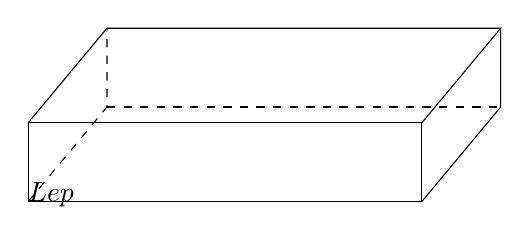
\begin{tikzpicture}
      % Parallelepipede
      \draw (0,0)--(5,0)--(5,1)--(0,1)--(0,0); % face
      \draw (0,1)--(1,2.2)--(6,2.2)--(5,1); % haut
      \draw (5,0)--(6,1.2)--(6,2.2); % côté
      % Perspective
      \draw[dashed] (0,0)--(1,1.2)--(1,2.2); % côté
      \draw[dashed] (1,1.2)--(6,1.2); % fond
      % Legendes
      \tkzVecteur(0)[5](-0.25){$L$}[below]*
      \tkzVecteur(-0.25)(0)[1]{$e$}[left]*
      \tkzVecteur(5.25)[1](-0.1)[1.2]{$p$}[right]*
    \end{tikzpicture}
  \end{multicols}
  Si $L$, $p$ et $e$ sont mesurées en \unit{\cm},
  le résultat s’exprimera en \unit{\cubic\cm}.
\end{doc}

\mesure Mesurer la masse volumique d'un échantillon à l'aide du matériel disponible.

\question{
  En utilisant le document~\ref{doc:TP3_proprietes_metaux}, déterminer la nature de l'échantillon.
}{
  On a mesuré un volume $V = 10,0 \times 2,0 \times \qty{0.2}{\centi\m\cubed} = \qty{4,0}{\centi\m\cubed}$ et une masse $m = \qty{34,0}{\g}$.
  L'échantillon a donc une masse volumique 
  \begin{equation*}  
    \rho
    = \dfrac{30,0}{4,0}\unit{\g/\cubic\centi\m}
    = \qty{7,5}{\g/\cubic\centi\m}
  \end{equation*}

  Comme l'échantillon est brillant et gris, on en déduit qu'on a du fer.
}{2}



%%%% Contexte 2
\begin{importants}
  Les eaux minérales sont des mélanges homogène contenant plusieurs ions de nature et de masses différentes.
  Les eaux minérales sont en général impropre à une consommation régulière, mais elles peuvent servir dans des régimes spécifiques.
  
  \problematique{Comment déterminer les ions présents dans des eaux minérales ?}
\end{importants}



%%%% documents
\begin{doc}{Composition de trois eaux minérales}{doc:TP3_composition_eau}
  \begin{multicols}{3}
    \centering
    \textbf{Vichy St Yorre} \\ \vspace*{-20pt}
    \begin{tableau}{l | r}
      \SetCell[c=2]{c} Minéralisation : \unit{\mg} pour \qty{1}{\litre} \\
      \ionBicarbonate & \num{4368} \\
      \ionChlorure    & \num{322}  \\
      \ionSodium      & \num{1708} \\
      \ionSulfate     & \num{174}  \\
      \ionPotassium   & \num{110}  \\
      \ionCalcium     & \num{90}   \\
      \ionFluorure    & \num{1}    \\
      \ionMagnesium   & \num{11}   \\
    \end{tableau}

    %
    \textbf{Mont Roucous} \\ \vspace*{-20pt}
    \begin{tableau}{l | r}
      \SetCell[c=2]{c} Minéralisation : \unit{\mg} pour \qty{1}{\litre} \\
      \ionBicarbonate & \num{1} \\
      \ionChlorure    & \num{2}  \\
      \ionSodium      & \num{3,2}  \\
      \ionSulfate     & \num{6,9}  \\
      \ionFluorure    & < \num{0,1}  \\
      \ionCalcium     & \num{2,7}  \\
      \ionNitrate     & \num{1,8}  \\
      \ionMagnesium   & \num{0,3}  \\
    \end{tableau}
    
    %
    \textbf{Cristalline} \\ \vspace*{-20pt}
    \begin{tableau}{l | r}
      \SetCell[c=2]{c} Minéralisation : \unit{\mg} pour \qty{1}{\litre} \\
      \ionBicarbonate & \num{228} \\
      \ionChlorure    & \num{15}    \\
      \ionSodium      & \num{8,4}  \\
      \ionSulfate     & \num{11}  \\
      \ionPotassium   & \num{2,3}     \\
      \ionCalcium     & \num{549}   \\
      \ionNitrate     & < \num{1}   \\
      \ionMagnesium   & \num{6,9}   \\
    \end{tableau}

    %
    % \textbf{Volvic\vphantom{p}} \\
    % \begin{tableau}{l | r}
    %   \SetCell[c=2]{c} Minéralisation : \unit{\mg} pour \qty{1}{\litre} \\
    %   \ionBicarbonate & \num{65,3} \\
    %   \ionChlorure    & \num{8,4}  \\
    %   \ionSodium      & \num{9,4}  \\
    %   \ionSulfate     & \num{6,9}  \\
    %   \ionPotassium   & \num{5,7}  \\
    %   \ionCalcium     & \num{9,9}  \\
    %   \ionNitrate     & \num{6,3}  \\
    %   \ionMagnesium   & \num{6,1}  \\
    % \end{tableau}
    % 
    % %
    % \textbf{Hépar} \\
    % \begin{tableau}{l | r}
    %   \SetCell[c=2]{c} Minéralisation : \unit{\mg} pour \qty{1}{\litre} \\
    %   \ionBicarbonate & \num{383,7} \\
    %   \ionChlorure    & \num{11}    \\
    %   \ionSodium      & \num{14,2}  \\
    %   \ionSulfate     & \num{1479}  \\
    %   \ionPotassium   & \num{4}     \\
    %   \ionCalcium     & \num{549}   \\
    %   \ionNitrate     & \num{4,3}   \\
    %   \ionMagnesium   & \num{119}   \\
    % \end{tableau}
  \end{multicols}
\end{doc}


%%%%
\begin{doc}{Tests caractéristiques de certains ions}{doc:TP3_tests_ions}
  \begin{center}
    \begin{tableau}{| c | c | c |}
      Ion à tester &
      Réactif utilisé &
      Résultat du test positif \\
      %
      \ionChlorure &
      Solution de nitrate d'argent &
      Précipité blanc, noircit* \\
      %
      \ionSulfate &
      Solution de chlorure de baryum &
      Précipité blanc \\
      %
      \ionCalcium &
      Solution d'oxalate d'ammonium &
      Précipité blanc \\
      %
      \ionMagnesium &
      Solution d'hydroxyde de sodium &
      Précipité blanc
    \end{tableau}
    
    \bigskip
    * Le précipité blanc noircit à la lumière.
  \end{center}
\end{doc}


%%%%
On a trois béchers (A, B, C) contenant des eaux minérales, que vous voulez identifier.

\mesure
Réaliser le protocole suivant :
\begin{protocole}
  \item Verser dans 4 tubes à essais quelques \unit{\mL} d'eau d'un bécher.
  \item Réaliser un test différent dans chaque tube à essais à l'aide des 4 réactifs.
  \item Noter si un précipité se forme et son abondance dans le tableau suivant ($-$, $+$, $++$, $+++$).
  \item Répéter pour les deux autres bécher.
\end{protocole}

\begin{center}
  \begin{tableau}{|l | c | c | c|}
    Test réalisé & Bécher A & Bécher B & Bécher C \\
    Nitrate d'argent    & & & \\
    Chlorure de baryum  & & & \\
    Oxalate d'ammonium  & & & \\
    Hydroxyde de sodium & & &
  \end{tableau}
\end{center}

\question{
  En utilisant les documents~\ref{doc:TP3_composition_eau} et~\ref{doc:TP3_tests_ions}, donner l'eau minérale contenue dans chaque bécher.
}{
  
}{3}

  % %%%%
\teteSndCorp

%%%% titre
\vspace*{-36pt}
\numeroActivite{1}
\titreActivite{Composition de l'atmosphère}


%%%% objectifs
\begin{objectifs}
  \item Comprendre comment on décrit la composition d'un mélange.
  \item Connaître la composition de l'air.
\end{objectifs}

\begin{contexte}
  L'atmosphère est un mélange de plusieurs gaz : dioxygène, diazote, dioxyde de carbone, etc.
  
  \problematique{
    Comment décrire la composition d'un mélange ?
  }
\end{contexte}


%%%% docs
\begin{doc}{Fraction volumique}{doc:A1_fraction_volumique}
  Soit une espèce chimique $E$ de volume $V_E$, dans un mélange de volume total $V$.
  La \important{proportion} ou \important{fraction volumique} de l'espèce chimique $E$ est
  \begin{equation*}
    p_{v}(E) = \frac{V_E}{V}
  \end{equation*}
  C'est une grandeur sans unité, comprise entre 0 et 1.
  On peut aussi l'exprimer en pourcentage, compris entre \qty{0}{\percent} et \qty{100}{\percent}.
  Par définition $\qty{10}{\percent} = \dfrac{10}{100} = \num{0,10}$.
\end{doc}

%%
\begin{doc}{Composition de l'atmosphère}{doc:A1_composition_atmo}
  \begin{importants}
    L’air contient \texteTrou[0.1]{\qty{78}{\percent}} de diazote \chemfig{N_2} et \texteTrou[0.1]{\qty{21}{\percent}} de dioxygène \chemfig{O_2}.
    Les autres gaz qui composent l’air sont l’argon \chemfig{Ar} (\qty{0,9}{\percent}),
    le dioxyde de carbone \chemfig{CO_2} (\qty{0,04}{\percent}),
    les gaz nobles et le méthane \chemfig{CH_4} (\qty{0,0002}{\percent}).
  \end{importants}
\end{doc}


%%%%
\question{
  Calculer le volume occupé par le diazote \chemfig{N_2} dans une salle de cours de \qty{600}{\metre\cubed}.
}{
  Le diazote occupe \qty{78}{\percent} du volume, soit $V_{\chemfig{N_2}} = 0,78 \times \qty{600}{\metre\cubed} = \qty{468}{\metre\cubed}$.
}{2}

\question{
  Même question pour le dioxygène \chemfig{O_2}.
}{
  Cette fois $V_{\chemfig{O_2}} = 0,21 \times \qty{600}{\metre\cubed} = \qty{126}{\metre\cubed}$.

}{2}

\begin{doc}{Respiration et dioxyde de carbone}{doc:A1_respiration}
  Quand on respire, on inspire du dioxygène \chemfig{O_2} qui est transformé en dioxyde de carbone \chemfig{CO_2} que l'on expire.

  Pendant une séance de cours d'une heure, le volume de dioxyde de carbone \chemfig{CO_2} double à cause de la respiration, si la salle n'est pas aérée.
\end{doc}

\question{
  Calculer la proportion volumique de dioxyde de carbone \chemfig{CO_2} après une heure de cours.
}{
  Le volume de dioxyde de carbone a doublé, on a donc une proportion deux fois plus élevée, soit \qty{0,08}{\percent}.
}{3}


%%
\begin{doc}{Fraction massique}{doc:A1_fraction_massique}
  Soit une espèce chimique $E$ de masse $m_E$, dans un mélange de masse totale $m$.
  La \important{proportion} ou \important{fraction massique} de l'espèce chimique $E$ est
  \begin{equation*}
    p_{m}(E) = \frac{m_E}{m}
  \end{equation*}
  C'est une grandeur sans unité, comprise entre 0 et 1.
  On peut aussi l'exprimer en pourcentage, compris entre \qty{0}{\percent} et \qty{100}{\percent}.
\end{doc}

\begin{doc}{Cloche en bronze}{doc:A1_cloche_bronze}
  \begin{wrapfigure}[5]{r}{0.2\linewidth}
    \vspace*{-31pt}
    \centering
    \image{0.7}{images/photos/cloche_bronze.png}
  \end{wrapfigure}
  
  Les cloches traditionnelles des temples coréens sont en bronze.
  Le bronze est un \textbf{alliage}, un mélange homogène entre deux métaux.
  
  Le bronze est constitué de \qty{20}{\percent} d'étain \chemfig{Sn} et de \qty{80}{\percent} de cuivre \chemfig{Cu} en masse.

  Une cloche traditionnelle pèse plusieurs centaines de kilogramme.
\end{doc}


\question{
  Exprimer les proportions massiques du cuivre et de l'étain dans une cloche en bronze sous la forme d'une division entre deux entiers les plus petits possibles.
}{
  $\qty{20}{\percent} = \dfrac{20}{100} = \dfrac{1}{5}$ pour l'étain.
  $\qty{80}{\percent} = \dfrac{80}{100} = \dfrac{4}{5}$ pour le cuivre.
}{3}

\question{
  Calculer la masse cuivre dans une cloche traditionnelle de masse $m = \qty{500}{\kg}$
}{
  La masse de cuivre vaut $0,8 \times \qty{500}{\kg} = \qty{400}{\kg}$.
}{2}

\question{
  Même question pour l'étain.
}{
  La masse d'étain vaut $0,2 \times \qty{500}{\kg} = \qty{100}{\kg}$.
}{2}

\question{
  Est-ce que l'on pourrait calculer les fractions volumiques de cuivre et d'étain à partir des fractions massiques ?
}{
  Non, car on ne sait pas quel est le volume de la cloche, ni quels sont les volumes de cuivre et d'étain dans la cloche.
}{1}

  % %%%% début de la page
\teteSndCorp

%%%% titre
\nomPrenomClasse
\numeroActivite{4}
\titreTP{Séparer et identifier des espèces chimiques}


%%%% objectifs
\begin{objectifs}
  \item Réaliser et analyser une Chromatographie sur Couche Mince.
\end{objectifs}


%%%% evaluation
\begin{tableauCompetences}
  \centering APP &
  Rechercher et utiliser des informations dans un document.
  & & & & \\
  %
  \centering VAL &
  Comparer des valeurs mesurées avec des valeurs de références.
  & & & &
\end{tableauCompetences}



%%%% contexte
\begin{contexte}
  En Europe, les colorants alimentaires sont désignés par un préfixe E suivi d'un numéro.
  Ces colorants se retrouvent dans de nombreux produits.
  
  On cherche à déterminer les colorants présent dans du sirop à l'aide d'une \important{Chromatographie sur Couche Mince (CCM).}
\end{contexte}


%%%% document
\begin{doc}{Chromatographie sur Couche Mince (CCM)}{doc:TP4_CCM}
  \begin{wrapfigure}[11]{l}{0.5\linewidth}
    \centering
    \vspace*{-16pt}
    \image{0.7}{images/chimie/CCM/CCM_exp.png}
    
    \footnotesize{Schéma expérimental d'une CCM.}
  \end{wrapfigure}

  La \important{chromatographie sur couche mince (CCM)} permet de séparer et d'identifier des espèces chimiques présentes dans un mélange.

  Le principe est le suivant : on dépose les espèces à identifier sur une couche mince (plaque), appelée \important{phase stationnaire}, dont on fait tremper une partie dans un \important{éluant}.
  
  Par capillarité, cet éluant va monter le long de la plaque, on parle de \important{phase mobile.}
  Les espèces déposées sur la plaque vont être entraînées par cette phase mobile.
  
  En fonction de leur affinités, les espèces chimiques monteront plus ou moins haut sur la plaque, ce qui permettra de les identifier.
  La fiche ainsi formée est appelée \important{chromatogramme}.
\end{doc}

%%%%
\begin{doc}{Réalisation d'une CCM}{doc:TP4_protocole_CCM}
  \begin{multicols}{3}
    \begin{center}
      \includegraphics[height=0.15\textheight]{images/chimie/CCM/CCM_etapes_cuve.png}
      
      Remplir jusqu'à environ \qty{0,5}{\cm} de hauteur d'éluant la cuve à CCM.
    \end{center} 
    
    \begin{center}
      \includegraphics[height=0.15\textheight]{images/chimie/CCM/CCM_etapes_trait.png}
      
      Tracer au crayon à papier un trait à \qty{1}{\cm} du bord inférieur.
    \end{center}
  
    \begin{center}
      \includegraphics[height=0.15\textheight]{images/chimie/CCM/CCM_etapes_depot.png}
      Marquer des emplacements,
      puis prélever chaque échantillon avec un cure dent et les déposer sur un des emplacements.
    \end{center}
  \end{multicols}
  
  \bigskip
  
  \begin{multicols}{2}
    \begin{center}
      \includegraphics[height=0.25\textheight]{images/chimie/CCM/CCM_etapes_ajout.png}
      
      Poser doucement la plaque dans la cuve en la tenant par les côtés et fermer la cuve.
      \important{Ne jamais déplacer la cuve} et attendre que l'éluant monte.
    \end{center}

    \begin{center}
      \includegraphics[height=0.25\textheight]{images/chimie/CCM/CCM_etapes_retrait}
      
      Quand le front de l'éluant s'approche du haut, sortir la plaque.
      Tracer une ligne indiquant la hauteur où l'éluant est monté.
    \end{center}
  \end{multicols}
\end{doc}


%%%% questions
\mesure
Placer un M\&M's dans chaque tube à essais et les recouvrir d'eau.
Attendre que le colorant se soit dissous dans l'eau et récupérer les M\&M's.

\mesure
Réaliser le protocole du document~\ref{doc:TP4_protocole_CCM}, avec un dépôt de colorant jaune, un dépôt de colorant bleu et deux dépôts des solutions préparées précédemment.

\mesure
Coller ici le chromatogramme \important{sec} et entourer les différentes tâches au crayon à papier.
\pasCorrection{\vspace*{9.25cm}}

\question{
  Pourquoi doit-on placer la ligne de dépôt au dessus du niveau de l'éluant ?
}{
  Si on la place en dessous, le dépôt va se diluer dans l'éluant et ne montera pas sur la plaque.
}{2}

\question{
  Pourquoi ne doit-on pas déplacer la cuve pendant la montée de l'éluant ?
}{
  Si on déplace la cuve, l'éluant va monter de manière irrégulière, ce qui va fausser l'analyse des résultats.
}{2}


%%%%
\pasCorrection{\newpage}
\begin{doc}{Lecture d'un chromatogramme}{doc:TP4_lecture_chromato}
  \begin{multicols}{2}
    \begin{listePoints}
      \item \important{Lecture verticale :} si le dépôt d'un échantillon se sépare en plusieurs tâches, il s'agit d'un mélange.
      \item \important{Lecture horizontale :} sur une même plaque, une même espèce chimique migre toujours à la même hauteur.
    \end{listePoints}
    \vfill \strut

    \centering
    \image{0.7}{images/chimie/CCM/chromatogramme_TP.png} \\
    \footnotesize{schéma d'un chromatogramme}
  \end{multicols}
\end{doc}

%%%%
\begin{doc}{Colorants alimentaires}{doc:TP4_colorants_alimentaire}
  \begin{listePoints}
    \item \important{E102 : jaune de tartrazine.} Son usage doit s'accompagner en France de la mention \og peut avoir des effets indésirables sur l'activité et l'attention chez les enfants \fg.
    \item \important{E133 : bleu brillant.} Un enfant de 40 kg peut ingérer jusqu'à $240\unit{mg}$ de bleu brillant en une journée. Au-delà le conseil européen indique que ce produit peut être toxique.
  \end{listePoints}
\end{doc}

\question{
  En analysant le chromatogramme à l'aide du document~\ref{doc:TP4_lecture_chromato}, indiquer si les échantillons sont des corps purs ou des mélanges.
}{
  Pour le bleu et le jaune, on a des corps purs (une seule tâche).
  Pour le vert on a un mélange, car le dépôt s'est séparé en deux tâches.
}{4}

\question{
  En utilisant le chromatogramme, donner la composition des colorants présents sur la couche externe des M\&M's.
}{
  Le jaune et le bleu du M\&M's montent à la même hauteurs que les dépots de colorant jaune E102 et bleu E133, ce sont donc les mêmes espèces chimiques.
}{6}


\pasCorrection{\newpage}
%%%% Contexte
\begin{contexte}
  Les huiles essentielles sont obtenues à partir de végétaux pressés ou par distillation fractionnée.
  Les huiles essentielles sont riches en molécules odorantes.
  
  \problematique{
    Comment décrire la composition d'une huile essentielle à l'aide d'une CCM ?
  }
\end{contexte}


%%%% docs
\separationBlocs{
  %%
  \begin{doc}{Huile essentielle de citron et d'orange}{doc:TP4_huile_essentielle}
    L'huile essentielle d'orange (HEO) et l'huile essentielle de citron (HEC)
    sont obtenues en pressant les zestes d'une orange et d'un citron respectivement.
  \end{doc}
}[0.31]{
  %%
  \begin{doc}{Odorat et molécules odorantes}{doc:TP4_molecules_odorantes}
    Chez les humains, Les molécules odorantes sont captées par des neurones de l’épithélium olfactif,
    puis ces neurones transmettent l'information nerveuse au cerveau qui y associe une odeur.
  
    Voilà quelques exemples de molécules odorantes :
    \begin{listePoints}
      \item le \important{limonène} (LIM), est associé à une odeur d'orange.
      \item le \important{linalol} (LIN), est associé à une odeur fraiche et florale.
      \item le \important{géraniol} (G), est associé à une odeur de rose.
      \item le \important{citral} (C), est associé à une odeur de citron.
    \end{listePoints}
  \end{doc}
}[0.69]


%%%%
\question{
  Quelles molécules odorantes peut-on trouver dans l'huile essentiel de citron et d'orange ?
}{
  D'après les descriptions du document~\ref{doc:TP4_molecules_odorantes},
  on s'attend à trouver du limonène dans l'huile essentielle d'orange et du citral dans l'huile essentielle de citron.
}{2}

\begin{doc}{Résultat d'une CCM}{doc:TP4_HEC_HEO}
  On a réalisé deux CCM pour déterminer la composition des huiles essentielles d'orange et de citron.
  \begin{center}
    \image{0.25}{images/donnees/chromato_HEC}
    \image{0.25}{images/donnees/chromato_HEO}
  \end{center}
\end{doc}

\question{
  En analysant les chromatogrammes, donner la composition de l'HEC et l'HEO.
}{
  On trouve du limonène, du géraniol et du citral dans l'HEC (tâches à la même hauteur).
  On trouve du limonène et du géraniol dans l'HEO.
}{5}

  % %%%%
\teteSndCorp

%%%% titre
%\vspace*{-36pt}
\numeroActivite{2}
\titreActivite{Mesure de la masse volumique de l'air}


%%%% objectifs
\begin{objectifs}
  \item Calculer la masse volumique de l'air.
\end{objectifs}

\begin{contexte}
  L'atmosphère est un mélange de plusieurs gaz : dioxygène, diazote, dioxyde de carbone, etc.
  
  \problematique{
    Comment calculer la masse volumique de l'air à partir de sa composition ou d'une expérience ?
  }
\end{contexte}


%%%% docs
\begin{doc}{Mesure de la masse volumique de l'air}{doc:A2_masse_volumique_air}
  \begin{wrapfigure}{r}{0.1\linewidth}
    \vspace*{-29pt}
    \qrcode{https://www.youtube.com/watch?v=isEo51ncsKU&t=26s}
  \end{wrapfigure}
  On peut mesurer la masse volumique de l'air en dégonflant un ballon dans une bouteille d'eau.
  La bouteille d'eau permet de mesurer le volume d'air expulsé.
  En pesant le ballon avant et après le dégonflage, on peut calculer la masse d'air expulsée.
\end{doc}

\numeroQuestion 
Schématiser les 3 étapes de l'expérience réalisée.
\vspace*{200pt}

\numeroQuestion
Remplir le tableau ci-dessous 
\begin{tableau}{|c |c |c |c |}
  Grandeur & Masse du ballon plein $m_1 $ & Masse du ballon dégonflé $m_2$ & Volume d'air expulsé $V$ \\
  \SetCell{couleurPrim!10} Valeur & \vphantom{$\dfrac{1}{2}$} & &
\end{tableau}

\question{
  Calculer la masse volumique mesurée $\rho_\text{mes}(\text{air})$.
}{}{3}

%%
\begin{doc}{Masse volumique d'un mélange}{doc:A2_composition_atmo}
  Pour un mélange de gaz, la masse volumique du mélange est simplement la somme des masses volumique de chaque gaz pondérée par la fraction volumique de chaque gaz du mélange.

  Pour l'air, on aura donc
  \begin{equation*}
    \rho(\text{air}) = p_v(\chemfig{O_2}) \rho(\chemfig{O_2}) + p_v(\chemfig{N_2}) \rho(\chemfig{N_2}) + p_v(\chemfig{Ar}) \rho(\chemfig{Ar}) + p_v(\chemfig{CO_2}) \rho(\chemfig{CO_2})
  \end{equation*}
\end{doc}

\newpage
\question{
  Rappeler les fractions volumique des gaz composant l'air (\chemfig{O_2}, \chemfig{N_2}, \chemfig{CO_2}, \chemfig{Ar}).
}{}{2}

\begin{doc}{Masse volumique des gaz composant l'air}{doc:A2_masse_volumique_air}
  \textbf{Données :}
  \begin{listeTirets}
    \item Masse volumique du \chemfig{CO_2} gazeux : $\rho(\chemfig{CO_2}) = \qty{1,87}{\g/\litre}$.
    \item Masse volumique du \chemfig{O_2}  gazeux : $\rho(\chemfig{O_2})  = \qty{1,35}{\g/\litre}$.
    \item Masse volumique du \chemfig{N_2}  gazeux : $\rho(\chemfig{N_2})  = \qty{1,18}{\g/\litre}$.
    \item Masse volumique de \chemfig{Ar}   gazeux : $\rho(\chemfig{Ar})   = \qty{1,78}{\g/\litre}$.
  \end{listeTirets}
\end{doc}


%%%%
\question{
  Calculer la masse volumique théorique de l'air $\rho_\text{theo}(\text{air})$.
}{
}{4}

\question{
  Comparer la valeur théorique et la valeur mesurée. Est-ce qu'elles sont égales ? Est-ce qu'elles sont cohérentes ?
}{}{2}
  %% Solutions
  % %%%% début de la page
\teteSndSolu

%%%% titre
\vspace*{-36pt}
\numeroActivite{1}
\titreTP{Dosage du sucre par étalonnage}

%%%% objectifs
\begin{objectifs}
  \item Apprendre le vocabulaire sur les solutions.
  \item Comprendre la notion de concentration massique
  \item Comprendre le principe de la dilution et de la dissolution
\end{objectifs}


%%%% contexte
\begin{contexte}
  Le sucre couramment présent dans notre alimentation est le saccharose.
  Cette espèce chimique peut entraîner des risques pour la santé si on en consomme trop.
  Il est donc important de pouvoir déterminer la quantité de sucre consommée par jour.

  \problematique{Comment déterminer la masse de saccharose présent dans un sirop ?}
\end{contexte}


%%%% documents
\begin{doc}{Solution, solvant et soluté}{doc:TP1_solution}
  \begin{encart}
    \chevron Une \important{solution} est un mélange homogène. \\
    Le \important{solvant} est le composant majoritaire du mélange.
    Les \important{solutés} sont les espèces qui sont dispersées dans le solvant.
  \end{encart}
  
  \begin{center}
    \important{Solvant + Soluté(s) = Solution}
  \end{center}
  
  \begin{encart}
    On parle de \important{solution aqueuse} si le solvant est l'eau \chemfig{H_2 O}.
  \end{encart}
\end{doc}

\begin{doc}{Composition d'un sirop}{doc:TP1_sirop}
  Le constructeur annonce que le sirop est composé d'\textit{eau}, de \textit{sucre} de \textit{jus de citron} et d'\textit{acide citrique} principalement.
\end{doc}


\question{
  Donner le solvant et les solutés présents dans le sirop.
}{}{2}


%%%%
\begin{doc}{Concentration en soluté}{doc:TP1_concentration}
  \begin{encart}
    La \important{concentration massique $\mathbf{c}$} mesure la quantité de soluté présent dans une solution.
    C'est le rapport de la masse $m$ de \textbf{soluté} dissous dans le volume $V$ de la \textbf{solution}
    \begin{equation*}
      c = \frac{m_\text{soluté}}{V_\text{solution}}
    \end{equation*} 
  \end{encart}
  % \attention Il faut bien distinguer \textbf{concentration massique} et \textbf{masse volumique}.
  % La concentration mesure la masse de soluté contenue dans une solution.
  % La masse volumique mesure la masse d'un échantillon contenue dans un volume donné.
\end{doc}


\begin{doc}{Dissolution du sucre dans l'eau}{doc:TP1_protocole_dissolution}
  \begin{protocole}
      \item Peser une masse donnée de sucre avec une balance de précision.
      \item Mettre le sucre dans une fiole jaugée de 50 mL.
      \item Compléter la fiole jaugée jusqu'à mi-hauteur avec de l'eau distillée, agiter.
      \item Compléter jusqu'au trait de jauge avec de l'eau distillée.
      \item Verser le mélange dans un bêcher de 100 mL.
  \end{protocole}
\end{doc}


%%%% questions
\newpage
\vspace*{-28pt}

\mesure
En utilisant le Document~\ref{doc:TP1_protocole_dissolution}, préparer un mélange de \qty{50}{\ml} d'eau et de de sucre.

\mesure
Mesurer et noter la masse volumique du mélange préparé $\rho =$ \texteTrou[0.1]{\qty{0,15}{\g/\ml}}

\question{
  Calculer la concentration massique de sucre dans la solution aqueuse préparé.
}{}{1}


%%%%
\begin{doc}{Mesure de concentration}{doc:TP1_dosage}
  \begin{encart}
    On parle de \important{dosage} quand on mesure la concentration d'une espèce chimique présente dans une solution.
  \end{encart}
  \begin{encart}
    Un \important{dosage par étalonnage} consiste à déterminer la concentration d’une espèce chimique en comparant une grandeur physique caractéristique de la solution, à la même grandeur physique mesurée pour des solutions étalon.
  \end{encart}
\end{doc}
 
\numeroQuestion 
En utilisant le papier millimétré, tracer la masse volumique en fonction de la concentration massique de sucre dans l'eau.

\numeroQuestion
En déduire la concentration massique de sucre dans la sirop $c_\text{sirop} =$ \texteTrou[0.1]{\qty{0,6}{\g/\ml}}


%%%%
\begin{doc}{Principe d'une dilution}{doc:TP1_principe_dilution}
  \begin{wrapfigure}[5]{r}{0.5\linewidth}
    \vspace*{-48pt}
    \centering
    \begin{multicols}{4}
    \image{1}{images/chimie/protocoles/dilution0001} \\[-12pt]
    \footnotesize{$S_0$}
    
    \image{1}{images/chimie/protocoles/dilution0002}
    
    \image{1}{images/chimie/protocoles/dilution0003}
    
    \image{1}{images/chimie/protocoles/dilution0004} \\[-12pt]
    \footnotesize{$S_1$}
    \end{multicols}
  \end{wrapfigure}
  \vAligne{-40pt}
  
  \begin{encart}
    Le principe de la \important{dilution} est de \important{diminuer la concentration} en soluté dans une solution en rajoutant du \important{solvant.}
  \end{encart}
  La solution de départ est appelée \important{solution mère}, notée $S_0$.
  La solution obtenue après dilution est appelée \important{solution fille}, notée $S_1$.

  Pour diluer une solution, il faut
  \begin{protocole}
    \item Prélever un volume $V_0$ de la solution à l'aide de la pipette graduée.
    Le bas du ménisque doit atteindre la graduation supérieure.
    \item Introduire la solution prélevée dans la fiole jaugée de volume $V_1$.
    \item Ajouter de l'eau distillée dans la fiole jaugée jusqu'aux $2/3$ et agiter doucement. Compléter jusqu'à ce que le bas du ménisque atteigne le trait de jauge.
    \item Fermer la fiole et l'agiter en la retournant plusieurs fois.
    \item Verser la solution fille obtenue dans un bécher.
  \end{protocole}
\end{doc}


%%%%
\begin{doc}{Facteur de dilution}{doc:TP1_dilution}  
  Le \important{facteur de dilution} est le rapport du volume de la solution fille sur le volume de la solution mère
  \begin{equation*}
    F = \frac{V_\text{1}}{V_\text{0}}
  \end{equation*}
  On dit qu'on a dilué $F$ fois une solution.
\end{doc}

\mesure 
Diluer \textbf{2 fois} le sirop et mesurer sa masse volumique. 

\numeroQuestion
En déduire la concentration massique en sucre.
Que constatez-vous ?
  % \input{seconde/solution/soluA1_dissolution}
  % %%%% début de la page
\teteSndSolu


%%%% titre
\vspace*{-36pt}
\numeroActivite{2}
\titreTP{Dosage d'un antiseptique}


%%%% objectifs
\begin{objectifs}
  \item Comprendre la notion de concentration massique.
  \item Doser la quantité de permanganate de potassium présente dans du Dakin.
\end{objectifs}


%%%% contexte
\begin{contexte}
  Le Dakin est une solution antiseptique qui sert à nettoyer des plaies. Le principe actif du Dakin est stabilisé par l'ajout de permanganate de potassium \chemfig{KMnO_4}.
  Le permanganate de potassium donne une teinte violette au Dakin.
  
  \problematique{Comment mesurer la concentration en \chemfig{KMnO_4} dans le Dakin ?}
\end{contexte}


%%%%
\begin{doc}{Concentration en soluté}{doc:TP2_concentration}
  \begin{importants}
    La \important{concentration massique $\mathbf{c}$} mesure la quantité de soluté présent dans une solution.
    C'est le rapport de la masse $m$ de \textbf{soluté} dissous dans le volume $V$ de la \textbf{solution}
    \begin{equation*}
      c = \frac{m_\text{soluté}}{V_\text{solution}}
    \end{equation*}
  \end{importants}
\end{doc}


%%%%
\begin{doc}{Dakin}{doc:TP2_dakin}
  Le Dakin est une solution aqueuse d'hypochlorite de sodium \chemfig{Na ClO}.
  Du permanganate de potassium \chemfig{K MnO_4} est ajouté à la solution, pour qu'elle ne soit pas dégradée par l'exposition au rayonnement UV du Soleil.
  
  \fleche Sur une bouteille de Dakin il est indiqué que la concentration de \chemfig{KMnO_4} vaut $\approx \qty{0,01}{\g/\litre}$.
\end{doc}

%
\question{
  Donner le solvant et les solutés de la solution de Dakin.
}{
  Le solvant est l'eau, les solutés sont le permanganate de potassium et l'hypochlorite de sodium.
}{2}


%%%%
\begin{doc}{Mesure de concentration d'une solution colorée}{doc:TP2_dosage}  
  \begin{importants}
    Une \important{échelle de teinte} permet de mesurer la concentration d'un soluté coloré.
  \end{importants}

  La teinte d'une solution est proportionnelle à la concentration en soluté.
  On prépare une série de solutions \textbf{étalons} dont on connaît la concentration et on compare leur teinte avec la solution dont on veut mesurer la concentration.
  
  \attention Il faut comparer les teintes avec des verreries identiques, la teinte s'assombrit avec l'épaisseur.
\end{doc}


%%%%
\begin{doc}{Protocole d'une dilution}{doc:TP2_protocole_dilution}
  \begin{wrapfigure}[5]{r}{0.5\linewidth}
    \vspace*{-32pt}
    \centering
    \begin{multicols}{4}
    \image{1.1}{images/chimie/protocoles/dissoDilu0007} \\[0pt]
    \footnotesize{$S_0$}
    
    \image{1.1}{images/chimie/protocoles/dissoDilu0008}
    
    \image{1.1}{images/chimie/protocoles/dissoDilu0010}
    
    \image{1.1}{images/chimie/protocoles/dissoDilu0011} \\[0pt]
    \footnotesize{$S_1$}
    \end{multicols}
  \end{wrapfigure}
  \vAligne{-40pt}
  
  \begin{importants}
    La \important{dilution} est la \important{diminution de la concentration} en soluté d'une solution en rajoutant du \important{solvant.}
  \end{importants}
  La solution de départ est appelée \important{solution mère}, notée $S_0$.
  La solution obtenue après dilution est appelée \important{solution fille}, notée $S_1$.

  Pour diluer une solution, il faut
  \begin{protocole}
    \item Prélever un volume $V_0$ de la solution à l'aide d'une pipette graduée.
    \textbf{Le bas du ménisque} doit atteindre la graduation supérieure.
    \item Introduire la solution prélevée dans la fiole jaugée de volume $V_1$.
    \item Ajouter de l'eau distillée dans la fiole jaugée jusqu'aux $2/3$ et agiter doucement.
    Compléter jusqu'à ce que \textbf{le bas du ménisque} atteigne le trait de jauge.
    \item Fermer la fiole et l'agiter en la retournant plusieurs fois.
    \item Verser la solution fille obtenue dans un bécher.
  \end{protocole}
\end{doc}

%%%%
\begin{doc}{Facteur de dilution}{doc:TP1_dilution}  
  Le \important{facteur de dilution} est le rapport du volume de la solution fille sur le volume de la solution mère et il est égal au rapport des concentrations des solutions mère et fille.
  \begin{equation*}
    F = \dfrac{V_1}{V_0} = \dfrac{c_0}{c_1}
  \end{equation*}
\end{doc}


%
\question{
  On souhaite réaliser une échelle de teinte composée de 4 solutions étalon pour mesurer la concentration de permanganate de potassium dans le Dakin.

  \begin{center}
    \begin{tblr}{c | X[1,c] | X[1,c] | X[1,c] | X[1,c]}
      Solution étalon & 1 & 2 & 3 & 4 \\ \hline
      Concentration (\unit{\g/\litre}) & \correction{\num{0,05}} & \correction{\num{0,025}} & \correction{\num{0,0125}} & \correction{\num{0,0063}} 
    \end{tblr}
  \end{center}
  
  Calculer le facteur de dilution entre les différentes solutions.
}{
  On divise par deux la concentration pour passer de la solution 1 à la solution 2, de la 2 à la 3 et de la solution 3 à la solution 4.
  Donc le facteur de dilution est $F = 2$.
}{1}

%
\question{
  Justifier l’intervalle des concentrations proposées pour l’échelle de teinte, à partir de la valeur attendue de la concentration en permanganate de potassium.
}{
  La valeur attendue de la concentration ($c = \qty{0,01}{\g/\litre}$) se trouve bien dans l'intervalle proposé.
}{1}

%
\question{
  Sachant que le volume de la fiole jaugée est $V_1 = \qty{50}{\ml}$, donner le volume de la solution mère $V_0$ à prélever pour avoir un facteur de dilution $F = 2$.
}{
  On doit avoir un volume deux fois plus faible, soit $V_0 = \qty{25}{\ml}$.
}{2}

%
\mesure
Réaliser l'échelle de teinte en effectuant trois dilutions successives.
Verser quelques millilitres de chaque solutions dans des tubes à essais.

%
\mesure
Utiliser l'échelle de teinte pour encadrer la valeur de la concentration en permanganate de potassium dans le Dakin.
Est-elle cohérente avec celle du constructeur ?
\pasCorrection{\lignesDeReponse{2}}
\correction{Oui, on trouve une concentration $\qty{0,0125}{\g/\litre} < c < \qty{0,0063}{\g/\litre}$.}

%
\question{
  Proposer une autre échelle de teinte pour améliorer la précision de la mesure (donner une liste de concentration).
}{
  On pourrait utiliser une échelle de teinte avec les concentrations suivantes : 0.015, 0.012, 0.0094, 0.0075, 0.006 \unit{\g/\litre} ($F = 1.25$).
}{1}

  % \input{seconde/solution/soluA2_dosage_sang}
  %% Mecanique
  % %%%% début de la page
\teteSndMouv

%%%%
\nomPrenomClasse


%%%% titre
\numeroActivite{1}
\titreTP{Décrire le mouvement}


%%%% objectifs
\begin{objectifs}
  \item Décrire un mouvement.
  \item Comprendre la notion de référentiel.
  \item Comprendre que le mouvement dépend du référentiel.
\end{objectifs}


%%%% evaluation
\begin{tableauCompetences}
  APP &
  Représenter une situation par un schéma avec une légende.
  & & & & \\
  %
  COM &
  Travailler en groupe, communiquer à l'oral.
  & & & & \\
\end{tableauCompetences}

%%%%
\vspace*{6pt}
\begin{doc}{Un peu de vocabulaire}{doc:TP1_vocabulaire}
  \begin{importants}
    \important{Système} : objet dont on étudie le mouvement.
  \end{importants}
  
  \begin{importants}
    \important{Trajectoire} : ensemble des positions successives occupées par le système.
  \end{importants}
  
  Le \important{mouvement} d'un système est donné par la description de sa trajectoire et de l'évolution de sa vitesse.
\end{doc} 


\begin{doc}{Type de trajectoires}{doc:TP1_trajectoires}
  Trajectoire \important{rectiligne} : \texteTrou{trajectoire représentée par une droite.}
  
  \texteTrou[0.5]{Trajectoire circulaire} : trajectoire représentée par un cercle.
  
  Trajectoire \important{curviligne} : \texteTrou{trajectoire représentée par une courbe.}
\end{doc}


\begin{doc}{Vitesse et accéleration}{doc:TP1_vitesse}
  Vitesse \important{uniforme} (constante) : le système n’accélère pas.
  
  La vitesse augmente : \texteTrouLignes{le système accélère.}
  
  La vitesse diminue : \texteTrouLignes{le système décélère.}
  
  Si \texteTrou[0.5]{la vitesse est constante et nulle}, on dit que le système est \important{immobile}.
\end{doc}


%%%%

\numeroQuestion
Compléter les documents~\ref{doc:TP1_trajectoires} et~\ref{doc:TP1_vitesse}.

\fleche Pour la suite de cette activité, vous allez choisir entre l'étude du mouvement des oies ou de la Lune.
Vous présenterez ensuite les résultats de votre étude au reste de la classe à l'oral.

\fleche Vous rendrez ensuite une compte-rendu détaillée en suivant les questions sur le \important{mouvement que vous n'avez pas choisi.}
Il faudra donc être attentif à ce que disent vos camarades !


%%%%
\newpage
\titreSousSection{\'Etude du mouvement des oies}

Le compteur du bateau affiche une vitesse $v_\text{bateau} = \qty{3,6e1}{\km/\hour}$.

\vspace*{6pt}
\numeroQuestion Pour la personne qui filme les oies, quelle est la vitesse des oies ?

\numeroQuestion Pour une personne se trouvant sur la berge, quelle est la vitesse des oies ?

\numeroQuestion Schématiser la trajectoire des oies si on les observe depuis la berge.

\numeroQuestion Indiquer le mouvement des oies depuis le bateau et la berge.

%%
\titreSousSection{\'Etude du mouvement de la Lune}

La Lune tourne autour de la Terre à une vitesse $v_\text{Lune} = \qty{3,7e3}{\km/\hour}$
et la Terre tourne autour du Soleil à une vitesse $v_\text{Terre} = \qty{1,1e5}{\km/\hour}$.

\begin{figure}[!ht]
  \begin{subfigure}{0.48\linewidth}
    \centering
    \image{0.8}{images/mecanique/terre_lune.png}
    \caption{Point de vue centré sur la Terre}
    \label{fig:terre_lune}
  \end{subfigure}
  \begin{subfigure}{0.48\linewidth}
    \centering
    \image{0.8}{images/mecanique/terre_lune_soleil.png}
    \caption{Point de vue centré sur le Soleil}
    \label{fig:terre_lune_soleil}
  \end{subfigure}
\end{figure}

\vspace*{-6pt}
\numeroQuestion Depuis le point de vue centré sur la Terre, quelle est la vitesse de la Lune ?

\numeroQuestion Schématiser la trajectoire de la Lune depuis ce point de vue et indiquer son mouvement.

\numeroQuestion Peut-on décrire la vitesse de la Lune depuis le point de vue centré sur le Soleil ?

\numeroQuestion Schématiser la trajectoire de la Lune depuis ce point de vue.


%%%%
\titreSousSection{Notion de référentiel}

\question{
  Convertir la vitesse $v_\text{Lune}$ en \unit{\m/\s}.
  \textit{Rappel :} \qty{1}{\km} = \qty{e3}{\metre}, \qty{1}{\hour} = \qty{3,6e3}{\s}.
}{}{2}

\question{
  Quelle distance la Lune parcours pendant 1 seconde ?
  Comparer avec la longueur de sa trajectoire, qui est de \qty{2,4e6}{\km}.
}{}{1}

\question{
  Peut-on décrire la trajectoire de la Lune en l'observant pendant 1 seconde ?
}{}{2}

\question{
  Conclusion : pourquoi est-il important de définir le référentiel, qui est l’endroit où on se place et le temps passé à observer, avant d'étudier un mouvement ?
}{}{1} % 2h
  % %%%% début de la page
\teteSndMouv

%%%% titre
%\nomPrenomClasse
\numeroActivite{1}
\vspace*{-36pt}
\titreActivite{Modéliser le mouvement}


%%%% objectifs
\vspace{-10pt}
\begin{objectifs}
  \item Modéliser le système étudié par un point matériel.
  \item Comprendre que le mouvement dépend du référentiel choisi.
  \item Comprendre l'utilisation des vecteurs en physique.
\end{objectifs}


%%%% evaluation
% \begin{tableauCompetences}
%   COM & Travailler en groupe, échanger entre élèves.
%   & & & &
% \end{tableauCompetences}


%%%%
\vspace*{-12pt}
\titreSection{Système et référentiel}

%%%%
\vspace{-10pt}
\begin{doc}{Modèle du point matériel}{doc:A1_point_materiel}
  \begin{importants}
    \important{Système} : objet dont on étudie le mouvement.
  
    On ne va s'intéresser qu'au mouvement global du système.
    C'est pourquoi on va modéliser le système par
    \texteTrouLignes[2]{
      Un point de même masse que le système, localisé au centre de masse du système.
      C'est le \important{modèle du point matériel.}
    }
  \end{importants}

  \fleche Le modèle du point matériel revient à ignorer toute information sur la géométrie du système étudié. 
  Les éventuelles rotations et déformations ne sont donc pas prises en compte.
\end{doc}


\begin{tblr}{
    colspec = {X[1.5,c,m] | X[1,c,m] | X[2,c] | X[2,c] },
    row{1} = {couleurPrim!20}
  }
  Système & Centre de masse & Trajectoire & Informations perdues \\ \hline
  %
  {\image{1}{images/mecanique/point_balle_tennis.png} \\ Balle de tennis} &
  Centre de la balle & & \\ \hline
  %
  {\image{1}{images/mecanique/point_roue.jpg} \\ Roue} &
  Centre de la roue & & \\ \hline
  %
  {\image{1}{images/mecanique/point_humain_course.jpg} \\ Modèle d'humain} &
  Nombril & &
\end{tblr}

%%
\newpage
\vspace*{-34pt}
\begin{doc}{Référentiel}{doc:A1_referentiel}
  Pour décrire le mouvement, il faut pouvoir le repérer dans l’espace et dans le temps, pour ça on utilise un référentiel.
  
  \begin{importants}
    \important{Référentiel} : \texteTrouLignes[1]{
      objet de référence, muni d'un repère par rapport auquel on étudie le mouvement du système.
    }
  \end{importants}
  
  \begin{importants}
    La description du mouvement dépend du \important{référentiel} choisi.
    On appelle ça la \important{relativité} du mouvement.
  \end{importants}
\end{doc}


%%%%
\titreSection{Vecteur}

%%
\vspace*{-8pt}
\begin{doc}{Vecteur en physique}{doc:A1_vecteur}
  \begin{importants}
    \important{Vecteur} : objet mathématique représenté par un segment fléché $\longrightarrow$ et noté avec une lettre surmontée d'une flèche $\vv{v}$.
    
    Un vecteur contient quatre information : 
    \begin{multicols}{2}
      \begin{listePoints}
        \item \texteTrou{Une direction.}
        \item \texteTrou{Un sens.}
        \item \texteTrou{Une valeur, ou norme.}
        \item \texteTrou{Une origine.}
      \end{listePoints}
    \end{multicols}
  
    Un vecteur est \important{constant} si
    \texteTrouLignes[1]{sa norme, sa direction et son sens sont constants.}
  \end{importants}
  
  \fleche En physique on va se servir des vecteurs pour représenter différentes grandeurs :
  \texteTrouLignes[1]{vitesse, force, champ électromagnétique, aimantation, accéleration, etc.}
  
  \attention Un vecteur n'est \textbf{jamais} égal à un nombre, qui contient moins d'information.
\end{doc}

\begin{doc}{Opération sur les vecteurs}{doc:A1_operation_vecteur}
  Même si les vecteurs ne sont pas des nombres, on peut effectuer des \important{opérations} avec.
  Cette année on ne réalisera que des opérations graphique.
  \begin{multicols}{3}
    \centering
    \begin{boite}
      \vAligne{50pt}
    \end{boite}
    Addition
    
    \begin{boite}
      \vAligne{50pt}
    \end{boite}
    Multiplication par un nombre

    \begin{boite}
      \vAligne{50pt}
    \end{boite}
    Soustraction
  \end{multicols}

  \begin{importants}
    Le \important{vecteur nul}, noté $\vv{0}$, est le vecteur de valeur nulle.
    On l'obtient en soustrayant un vecteur par lui même $\vv{a} - \vv{a} = \vv{a} + (-1 \times \vv{a}) = \vv{0}$.
  \end{importants}
\end{doc} % 1h
  % \input{seconde/mecanique/mecaTP2_vitesse} % 2h
  % %%%% début de la page
\teteSndMouv


%%%% titre
\vspace*{-32pt}
\numeroActivite{2}
\titreActivite{Modéliser une action par une force}


%%%% objectifs
\begin{objectifs}
  \item Comprendre la notion de force
  \item Connaître des exemples de forces
\end{objectifs}

%%%%
\begin{doc}{Force et action mécanique}{doc:A2_action_force}
  \begin{encart}  
    Un corps exerce une \important{action mécanique} sur un système étudié \texteTrouLignes[1]{s’il est capable d’en modifier le mouvement.}
  \end{encart}
  
  Une action mécanique est modélisée par une \important{force.}

  \begin{encart}
    La force exercée par un corps $A$ sur un corps $B$ est représentée par un vecteur $\vvFAsurB$.
    Ce vecteur possède les caractéristiques suivantes :
    \begin{listePoints}
      \item Une \important{valeur} notée $\FAsurB$, qui s'exprime en newton noté \unit{\newton}.
      \item Une \important{direction} et un \important{sens} qui dépendent de la situation.
      \item Une \important{origine}, appelée \important{point d'application} : le centre du système $B$.
    \end{listePoints}
  \end{encart}
\end{doc}

\mesure
Une personne pousse un carton. 
Représenter la force $\vv{F}_\text{personne/carton}$ qu'exerce la personne sur le carton.

\vspace*{-8pt}
\begin{center}
  \image{0.23}{images/mecanique/personne_carton}
\end{center}


%%
\begin{doc}{Exemples de forces}{doc:A2_exemples_forces}
  On distingue 2 types d'actions :
  \begin{listePoints}
    \item les \important{actions de contact} (contact entre l’objet qui donne la force et l’objet qui la reçoit),
    \item les \important{actions à distance} (pas de contact).
  \end{listePoints}
  
  \begin{tblr}{
    colspec = {|c |c |X[c] |}, hlines,
    row{1} = { couleurPrim!20 },
  }
    Force & Valeur & Direction, sens \\
    %
    poids $\vv{P}$ &
    $P = m \times g$ &
    verticale, vers le bas \\
    %
    réaction du support $\vv{R}$ &
    égale au poids $R = P$ &
    perpendiculaire au support, vers le haut \\
    %
    frottements $\vv{f}$ &
    dépend du cas étudié &
    opposés à la vitesse $\vv{v}$ \\
  \end{tblr}
  \smallskip
  
  \begin{listePoints}
    \item $\vv{P}$ représente l'interaction gravitationnelle de la Terre.
    \item $\vv{R}$ représente l'action exercée par le support sur un objet posé dessus.
    \item $\vv{f}$ représentent l'action d'un milieu (gaz, liquide, support solide).
  \end{listePoints}
  \attention Si un objet est \important{immobile par rapport au milieu,} il n'y a pas de frottements.
\end{doc}

\vspace*{-16pt}
\question{
  Parmi les forces $\vv{P}$, $\vv{R}$ et $\vv{f}$, indiquer celles qui modélisent une action de contact et celles qui modélisent une action à distance.
}{}{3}


%%%%
\begin{center}
  \begin{tblr}{
    colspec = {|X[c,m] |X[c,m] |}, hlines,
    row{1,3} = {couleurPrim!20},
  }
    Ballon & Curling \\
    \image{0.8}{images/mecanique/ballon_football} &
    \image{0.8}{images/mecanique/curling} \\
    %
    Parachutiste & Skieuse \\
    \image{0.8}{images/mecanique/parachutiste} &
    \image{0.8}{images/mecanique/skieur} \\  
  \end{tblr}
\end{center}

%%
\mesure 
En vous aidant des documents~\ref{doc:A2_action_force} et~\ref{doc:A2_exemples_forces}, compléter le tableau :
\begin{listePoints}
  \item Schématiser la ou les forces entrant en jeu, en faisant attention à leurs points d'application.
  \item Tracer la somme de toutes les forces entrant en jeu.
\end{listePoints}



%%%%
% \titreSection{Principe d'inertie}

% \question{
%   Répondre par vrai ou faux en justifiant à l'aide d'exemples ou de contre exemples.
% }{}{0}

% \vspace*{-6pt}
% \question{
%   Si un objet est en mouvement, alors il est forcément accéléré.
% }{}{2}

% \question{Si un objet est en mouvement, alors il subit une force dans le sens du mouvement.}{}{2}

% \question{Si deux objets sont animés par les mêmes forces, alors ils suivent la même trajectoire.}{}{2}

% \question{
%   On dit que deux forces se compensent si leur sommes vectorielle est nulle.
%   Pour quels systèmes de la figure~\ref{tab:situations_sportives} les forces se compensent-elles ?
% }{}{2}

% \question{
%   Quel est le mouvement du système dans chaque cas où les forces se compensent ?
% }{}{2}



% \begin{doc}{Conclusion : Le principe d'inertie}
%   \phantom{b}
%   \vspace*{-12pt}
  
%   \chevron Le \important{principe d'inertie} a été formulé pour la première fois par Newton en 1687.
%   Newton s'appuyait sur les travaux de Descartes et de Galilée, et parfois on appelle ce principe la \important{première loi de Newton}.
%   Sa formulation moderne est la suivante :
  
%   \begin{encart}
%     Si les forces qui s'exercent sur un système se compensent, alors ce système est \\[6pt]
%     soit \lignePointillee{0.2}, 
%     soit en mouvement \dotfill
%   \end{encart}
  
%   \begin{encart}
%     Réciproquement, si un système est \dotfill \\[6pt]
%     .\dotfill, alors les forces\\[6pt]
%     . \dotfill
%   \end{encart}
% \end{doc}


% %%%%
% \titreSection{Variation du vecteur vitesse}

% \question{
%   Comment varie $\vv{v}$ pour un système qui a un mouvement rectiligne uniforme ?
%   En déduire la variation de $\vv{v}$ pour un système soumis à des forces qui se compensent.
% }{}{3}

% \begin{doc}{Principe d'inertie et vitesse}
%   \vspace*{-24pt}
%   \begin{encart}
%     Le principe d'inertie dit que si le vecteur vitesse \dotfill \\[6pt]
%     au cours de la trajectoire, alors \dotfill \\[6pt]
%     \reponse{1}
%     %les forces exercées sur le système se compensent.
%   \end{encart}
% \end{doc} % 2h
  % %%%% début de la page
\teteSndMouv


%%%% titre
\vspace*{-32pt}
\numeroActivite{3}
\titreActivite{Le principe d'inertie}


%%%% objectifs
\begin{objectifs}
  \item Comprendre la notion d'inertie
  \item Comprendre le principe d'inertie.
\end{objectifs}


\begin{doc}{Inertie d'un corps}{doc:A3_inertie}
  \begin{encart}
    \important{L'inertie} est la tendance qu'ont les corps à rester dans le même état (repos ou mouvement), en l'absence de forces appliquées.
  \end{encart}
    
  \fleche C'est la masse qui le mesure : plus un objet a une masse élevée et plus il a de l'inertie.
  
  \fleche Dis autrement : plus un objet est lourd, plus il faut exercer une force importante pour changer son mouvement.
  
  \exemple Faire rouler un caddie vide est très facile, mais c'est plus difficile quand il est plein !
\end{doc}


\begin{doc}{Forces qui se compensent}{doc:A3_forces_compensent}
  On dit que des forces se compensent si leur somme est égale au vecteur nul $\vv{0}$.

  Pour que la somme de deux vecteurs soit nulles, il faut qu'ils aient 
  \begin{listePoints}
    \item même direction,
    \item même valeur,
    \item mais un sens opposé.
  \end{listePoints}

  \centering
  \image{0.75}{images/mecanique/forces_systemes}
\end{doc}

\question{
  Pour quels systèmes du document~\ref{doc:A3_forces_compensent} les forces se compensent-elles ?
}{}{2}

\question{
  Quel est le mouvement du système dans chaque cas où les forces se compensent ?
}{}{2}



\begin{doc}{Conclusion : Le principe d'inertie}{doc:A3_principe_inertie}
  \chevron Le \important{principe d'inertie} a été formulé pour la première fois par Newton en 1687.
  Newton s'appuyait sur les travaux de Descartes et de Galilée, et parfois on appelle ce principe la \important{première loi de Newton}.
  Sa formulation moderne est la suivante :
  
  \begin{encart}
    Si les forces qui s'exercent sur un système se compensent, alors ce système est \texteTrouLignes[2]{soit immobile, soit en mouvement rectiligne uniforme.}
  \end{encart}
  
  \begin{encart}
    Réciproquement, si un système est
    \texteTrouLignes[3]{immobile ou en mouvement rectiligne uniforme, alors les forces qui s'exercent sur lui se compensent.}
  \end{encart}
\end{doc}


%%%%
\question{
  Comment varie $\vv{v}$ pour un système qui a un mouvement rectiligne uniforme ?
  En déduire la variation de $\vv{v}$ pour un système soumis à des forces qui se compensent.
}{}{3}

\begin{doc}{Principe d'inertie et vitesse}{doc:A3_principe_inertie_vitesse}
  \begin{encart}
    Le principe d'inertie dit que si le vecteur vitesse
    \texteTrouLignes[2]{
      est constant sur toute la trajectoire, alors les forces exercées sur le système se compensent.
    }
  \end{encart}
\end{doc} % 1h
  % %%%% début de la page
\teteSndMouv

%%
\nomPrenomClasse


%%%% titre
\numeroActivite{4}
\titreActivite{Principe des actions réciproques}


%%%% evaluation
\pasCorrection{
\vspace*{-8pt}
\begin{tableauCompetences}
  %
  \centering ANA/RAI &
  Analyser les forces qui s'exercent sur un système.
  & & & & \\
  %
  \centering REA &
  Schématiser une situation.
  & & & & \\
  %
  \centering COM &
  Travailler en groupe.
  & & & &
\end{tableauCompetences}
}


%%%% objectifs
\begin{objectifs}
  \item Analyser et schématiser un système en mouvement
  \item Utiliser le principe d'inertie
  \item Comprendre le principe des actions réciproques
\end{objectifs}


%%%%
\begin{doc}{Forces qui se compensent}{doc:A4_forces_compensent}
  \begin{importants}
    On dit que les forces exercées sur un système \important{se compensent}, si leur somme vectorielle est nulle (égale à $\vv{0}$ le vecteur de norme nulle).
    
    \begin{wrapfigure}{r}{0.4\linewidth}
      \vspace*{-40pt}
      \begin{center}
        \begin{tikzpicture}
          % système 
          \tkzCercle{0}{0}{gray!50!white}{20}
          \tkzPointLabel{0}{0}{$A$}
          % forces
          \tkzVecteur(0)[-1.7](0)[-0.75]{$\vv{F}_1$}[left]
          \tkzVecteur(0)[1.7] (0)[0.75] {$\vv{F}_2$}[right]
        \end{tikzpicture}
      
        $\vv{F}_1 + \vv{F}_2 = \vv{0}$, les forces exercée sur le système $A$ se compensent.
      \end{center}
    \end{wrapfigure}
    
    La somme de deux vecteurs est nulle s'ils ont
    
    \begin{listePoints}
      \item \important{même point d'application},
      \item \important{même direction},
      \item \important{même norme},
      \item mais des \important{sens opposés}.
    \end{listePoints}
  \end{importants}
\end{doc}


%%%%
\begin{doc}{Ballon lancé depuis un skateboard}{doc:A4_ballon}
  \begin{flushright}
    \vspace*{-18pt}
    \qrcode{https://youtu.be/Kf0bBxmNeec?t=99}
  \end{flushright}
  \begin{multicols}{3}
    \centering
    \image{0.9}{images/mecanique/lancer_balle_reciproque_1.jpg}
    
    Avant le lancer
    
    \image{0.9}{images/mecanique/lancer_balle_reciproque_2.jpg}

    Pendant le lancer
    
    \image{0.9}{images/mecanique/lancer_balle_reciproque_3.jpg}

    Après le lancer
  \end{multicols}
\end{doc}


%%%
\problematique{Quelle est la force qui met en mouvement la personne sur le skateboard ?}

\numeroQuestion
Étudier le mouvement du système $A$ \og personne sur le skateboard \fg\; et du système $B$ \og ballon \fg\; avant, pendant et après le lancer du ballon.

\numeroQuestion
Décrire les propriétés de la force qui met en mouvement le système $A$.

\fleche Vous Détaillerez soigneusement les étapes de vos raisonnements par écrits sur un compte-rendu complet, compréhensible par un-e élève qui n'aurait pas vu la vidéo.

%\feuilleBlanche % 2h
  % \input{seconde/mecanique/mecaA5_forces_gravitationnelle} % 1h
  % \input{seconde/mecanique/mecaA6_poids} % 1h
  % \input{seconde/mecanique/mecaA7_exercices} % 2h
  % \input{seconde/mecanique/mecaTP3_poids} % 2h
  %% Atome
  % \teteSndAtom

\titre{Plan de Travail -- \sndAtom}
  
\phantom{\methode}\vspace*{-24pt}

\begin{multicols}{2}
  \begin{activite}{Ordres de grandeur}{ordre_grandeur}
    \begin{objectifs}  
      \item Revoir les puissances de 10.
      \item Apprendre à raisonner en ordres de grandeur.
    \end{objectifs}
  \end{activite}

  \phantom{\sndAtom}\vspace*{-24pt}
  
  \begin{activite}{Fabriquer un atome}[1 h 30]{atome}
    \begin{objectifs}
      \item Étudier la composition d'un atome.
      \item Comprendre que le nombre de protons définit un élément chimique.
      \item Savoir distinguer un ion d'un atome.
    \end{objectifs}
  \end{activite}
  
  \begin{TP}{Le modèle de l'atome}{modele_atome}
    \begin{objectifs}
        \item Découvrir la méthode scientifique.
        \item Utiliser la méthode scientifique pour étudier l'évolution du modèle de l'atome.
    \end{objectifs}
  \end{TP}
  
  \begin{activite}{Taille d'un atome}{taille_atome}
    \begin{prerequis}
      \item Calcul avec les puissances de 10.
      \item Utilisation des ordres de grandeur.
    \end{prerequis}
    %
    \begin{objectifs}
      \item Comparer la taille d'un atome à des objets du quotidien pour mieux la comprendre.
      \item Utiliser les ordres de grandeurs pour mener un raisonnement.
    \end{objectifs}
  \end{activite}
\end{multicols}

\begin{multicols}{2}    
  \begin{activite}{Cortège électronique}[1 h 30]{cortege_electrons}
    \begin{prerequis}
      \item Connaître la structure d'un atome.
      \item Savoir qu'un atome a autant d'électrons qu'il a de protons.
    \end{prerequis}
    %
    \begin{objectifs}
      \item Comprendre que les électrons s'organisent en couches électroniques.
      \item Comprendre la règle de remplissage des couches électroniques.
    \end{objectifs}
  \end{activite}

  \phantom{\strut}
  
  \begin{TP}{Le Tableau périodique}{tableau_periodique}
    \begin{prerequis}
      \item Connaître la structure électronique.
      \item Savoir remplir les couches et sous-couches électronique d'un atome.
    \end{prerequis}
    \begin{objectifs}
      \item Comprendre la construction du tableau périodique.
    \end{objectifs}
  \end{TP}
\end{multicols}
    
  \begin{tikzpicture}
  [overlay, remember picture, line width=1mm, draw=couleurQuat]
    \draw[->, rounded corners=4mm] 
      (ordre_grandeur) 
      to (5, 18.5) to (8, 17.8) 
      to (taille_atome);
    \draw[->] (atome) -- (cortege_electrons);
    \draw[->, rounded corners=5mm] 
      (cortege_electrons) 
      to (10, 2) 
      to (tableau_periodique);
  \end{tikzpicture}

\vspace*{-40pt}
\begin{tacheFinale}
  Choisir un élément du tableau périodique et réaliser sa case au format $20\times\qty{20}{\cm\squared}$.
  La case devra contenir des informations microscopique (structure électronique) et des informations macroscopique (dans quels objets on trouve l'élément, etc.)
\end{tacheFinale}
  % \input{seconde/atome/AtomA1_fabriquer_atome}
  % \input{seconde/atome/AtomA2_taille_atome}
  % \input{seconde/atome/AtomA3_modele_atome}
  % \input{seconde/atome/AtomA4_cortege_electronique}
  % \input{seconde/atome/AtomA5_tableau_periodique}
  %% Molécules
  % %%%%
\teteSndMole

%%%% titre
\vspace*{-36pt}
\numeroActivite{1}
\titreActivite{En quête de stabilité : les ions}


%%%% Objectifs
\vspace*{-8pt}
\begin{objectifs}
  \item Comprendre la règle du duet et de l'octet.
  \item Comprendre comment 
\end{objectifs}

\begin{contexte}
  Dans la nature la plupart des atomes vont spontanément perdre ou gagner des électrons pour former des ions.
  
  Seuls les gaz nobles de la 18$^\text{ème}$ colonne du tableau périodique (\chemfig{He}, \chemfig{Ne}, \chemfig{Ar}, \chemfig{Kr}, etc.) se trouvent le plus souvent sous forme de gaz monoatomiques.
  C'est parce qu'ils ont une grande stabilité, on dit qu'ils ont une grande inertie chimique.
  
  \problematique{
    Comment expliquer la formation d'ions monoatomique et la charge qu'ils portent à partir de la configuration électronique des gaz nobles ?
  }
\end{contexte}


%%%% question
\titreSection{Les gaz rares}

\numeroQuestion Compléter le tableau suivant

\begin{center}
  
  \begin{tableau}{|c | c | c | c |}
     Gaz noble &
     Numéro atomique & Nombre d'électrons &
     Configuration électronique \\
     Hélium \chemfig{He} & $Z = 2$  & & \\
     Néon \chemfig{Ne}   & $Z = 10$ & & \\
     Argon \chemfig{Ar}  & $Z = 18$ & & \\
  \end{tableau}
\end{center}

\question{
  Comment est la couche externe pour ces trois gaz nobles ?
}{}{2}


%%
\titreSection{La règle du duet et de l'octet}

Pour \important{augmenter leur stabilité,} les atomes adoptent la configuration électronique du gaz noble avec le numéro atomique le plus proche.
Ce principe se décompose en deux règles :

\begin{importants}
  \pointCyan \important{Règle du duet :} les atomes de numéro atomique $Z < 6$
  tendent à adopter la configuration électronique
  \texteTrouLignes{de l'hélium avec deux électrons : \important{1s$^2$}.}
  Ils ont \texteTrou{2 (un duet)} électrons sur leur couche externe. 
  \bigskip
  
  \pointCyan \important{Règle de l'octet :} les atomes de numéro atomique $Z > 6$
  tendent à adopter la configuration électronique externe du gaz noble le plus proche avec
  \texteTrouLignes{huit électrons : \important{ns$^2$ np$^6$}.}
  Ils ont \texteTrou{8 (un octet)} électrons sur leur couche externe.
\end{importants}


%%
\newpage
\titreSection{Les ions monoatomiques}

Pour adopter une configuration électronique plus stable, les atomes vont spontanément perdre ou gagner des électrons et ainsi former des ions.
\bigskip

\question{
  Le lithium \chemfig{Li} a pour numéro atomique $Z = 3$.
  Rappeler sa configuration électronique.
  Pour devenir stable, quelle règle doit-il respecter ? 
  Combien d'électrons doit-il perdre pour la respecter ?
  Quel ion formera-t-il ?
}{}{5}


\question{
  Mêmes questions pour le soufre \isotope{}{16}{S} ($Z = 16$).
}{}{5}


\question{
  Par analogie avec le soufre \isotope{}{16}{S}, pouvez-vous répondre simplement aux mêmes questions pour l'oxygène \isotope{}{8}{O} ?
}{}{5}


\question{
  Comment répondre à ces questions en regardant simplement le tableau périodique ?
}{}{5}
  % %%%%
\teteSndMole

%%%% titre
\numeroActivite{2}
\titreActivite{En quête de stabilité : formation des molécules}


%%%% Objectifs
\begin{objectifs}
  \item Comprendre la liaison covalente et les notions de doublet liant et non-liant.
  \item Comprendre que la stabilité d'une molécule est liée à la règle du duet et de l'octet (couche externe complète).
  \item Savoir analyser un schéma de Lewis pour expliquer la stabilité d'une molécule.
\end{objectifs}

\begin{contexte}
  En dehors des gaz nobles de la 18$^\text{ème}$ colonne du tableau périodique (\chemfig{He}, \chemfig{Ne}, \chemfig{Ar}, \chemfig{Kr}, etc.), les éléments ont tendance à s'associer spontanément pour former des molécules. 
  %Comme pour la formation des ions, les éléments gagnent en stabilité en complétant leur couche externe, en respectant la règle du duet ou de l'octet.
  
  \problematique{
    Quelles règles régissent la formation des molécules ?
  }
\end{contexte}


%%%% docs
\titreSection{Le modèle de Lewis}

\begin{doc}{Électrons de valences}{doc:A2_electron_valence}
  Les éléments ont tendance à s'associer en molécule, afin de gagner en stabilité en complétant leur couches électronique externe.  \begin{importants}  
    Les électrons de la couche externe sont appelés \important{électrons de valence.}
  \end{importants}  
\end{doc}
  
\begin{doc}{Doublet liant et liaison covalente}{doc:A2_doublet_liant}
  En 1916, Lewis propose un modèle simple pour schématiser la formation des liaisons entre éléments :
  \begin{importants}  
    Les éléments qui s'associent en molécule vont mettre en commun un des électrons de leur couche externe.
    Ces électrons mis en commun forment une paire appelée \important{doublet liant}.
  \end{importants}
  \begin{importants}  
    En partageant leurs électrons les éléments deviennent liés, on parle de \important{liaison covalente.}
  \end{importants}

  
  \exemple Formation de la molécule de dihydrogène \chemfig{H_2} à partir de deux éléments \isotope{}{1}{H} :
  
  \begin{center}
    {\small Schéma des deux éléments hydrogènes liés par un partage d'électron}
    \vspace{8pt}
    
    \image{0.2}{images/atomes/molecule_H2}
  \end{center}

  Pour représenter la molécule, on peut soit donner sa \important{formule brute}, soit son \important{schéma de Lewis :}
  \begin{multicols}{2}
    \begin{center}
      {\small Schéma de Lewis de la molécule}
      
      \image{0.4}{images/atomes/Lewis_H2}
    \end{center}

    \begin{center}
      {\small Formule brute de la molécule}

      \
      \chemfig{H_2}
    \end{center}
  \end{multicols}
\end{doc}

\question{
  Rappeler la configuration électronique de l’hydrogène \isotope{}{1}{H}, du carbone \isotope{}{6}{C}, de l’azote \isotope{}{7}{N} et de l'oxygène \isotope{}{8}{O}.
  Identifier pour chacun de ces atomes leurs électrons de valence.
}{}{5}

\question{
  Donner le nombre d'électrons manquant à chaque élément pour que leur couche externe soit pleine et qu'ils gagnent en stabilité.
}{}{3}

\question{
  Quelle molécule stable peut-on former à partir d'un carbone et de 4 hydrogènes ?
}{}{3}

\mesure Construire cette molécule à partir des modèle moléculaire.


\begin{doc}{Doublet non-liant}{doc:A2_doublet_non_liant}
  Lors de la formation d'une molécule, les électrons de valence qui ne sont pas partagés forment des paires appelées \important{doublet non-liant}.
  
  \exemple Formation de la molécule d'eau \chemfig{H_2 O} à partir de 2 atomes \isotope{}{1}{H} et d'un atome \isotope{}{8}{O} :
  \vspace{8pt}
  
  \separationBlocs{
    \begin{center}
      {\small Schéma des trois éléments se partageant des électrons}
      \vspace{8pt}
      
      \image{0.8}{images/atomes/molecule_H2O}
    \end{center}
  }{
    \begin{center}
      {\small Schéma de Lewis des doublets liants et des doublets non-liants (barres du haut)}
      \vspace{20pt}
      
      \image{0.4}{images/atomes/Lewis_H2O}
    \end{center}
  }
\end{doc}

\question{
  Indiquer combien de doublet non-liant la molécule d'eau possède.
}{}{2}

\newpage
\vspace*{-24pt}
\begin{doc}{Liaisons multiples}{doc:A2_liaisons_multiples}
  Pour être stables, les éléments peuvent partager plusieurs paires d’électrons et ainsi créer une liaison multiple.
  Celle-ci peut être double, comme dans le cas du dioxygène ; ou triple comme dans le cas du diazote.
  
  \centering
  \separationBlocs{
    \begin{center}
      {\small Schéma de Lewis}
      \vspace{36pt}
      
      \image{0.4}{images/atomes/Lewis_O2}
    \end{center}
  }{
    \begin{center}
      {\small Schéma des deux éléments oxygène se partageant des électrons}
      \vspace{8pt}
      
      \image{0.8}{images/atomes/molecule_O2}
    \end{center}
  }
  \vspace{12pt}
  
  \separationBlocs{
    \begin{center}
      {\small Schéma des deux éléments azote se partageant des électrons}
      \vspace{8pt}
      
      \image{0.8}{images/atomes/molecule_N2}
    \end{center}
  }{
    \begin{center}
      {\small Schéma de Lewis}
      \vspace{36pt}
      
      \image{0.4}{images/atomes/Lewis_N2}
    \end{center}
  }
\end{doc}


%%%% questions
\question{
  Quelle molécule peut-on former à partir d'un carbone, d'un d'oxygène et de plusieurs hydrogènes ?
}{}{3}

\mesure
Construire cette molécule à partir des modèles moléculaires.

\begin{doc}{Règles de stabilité}{doc:A2_regle_stabilite}
  \begin{importants}
    Pour gagner en stabilité, les éléments peuvent partager les électrons de leur couche externe en créant \important{des liaisons covalentes.}
    
    De cette manière, les éléments \texteTrouLignes[1]{complètent leur couche externe et sont donc plus stables.}
    
    Pour savoir combien de liaisons un élément peut former, il suffit de
    \texteTrouLignes[2]{compter le nombre d'électrons de valence et le nombre d'électrons manquant pour que la couche externe soit complète.}
  \end{importants}
\end{doc}

\begin{wrapfigure}{r}{0.1\linewidth}
  \vspace*{-18pt}
  \qrcode{https://mirage.ticedu.fr/?p=2324}
\end{wrapfigure}

\mesure Télécharger l'application mirage.

\mesure Au dos de la feuille, donner la formule brute de la molécule, son schéma de Lewis et vérifier que tous les éléments ont le bon nombre d'électrons.
  % %%%%
\teteSndMole

%%%% titre
\vspace*{-32pt}
\numeroActivite{1}
\titreTP{Dénombrer un grand nombre d'entités identiques}


%%%% Objectifs
\begin{objectifs}
  \item Comprendre qu'une \important{espèce chimique} est constituée d'un très (très) grand nombre \important{d'entités chimiques}.
  \item Comprendre l'utilité de compter les entités par paquets.
  \item Comprendre le concept de mole.
\end{objectifs}

\begin{contexte}  
  Les atomes, ions et molécules sont des entités chimique qui composent toute la matière macroscopique qui nous entoure.
  
  \problematique{
    Comment compter les \important{entité chimique} microscopique dans une \important{espèce chimique} macroscopique ?
  }
\end{contexte}


%%%%
\titreSection{Compter des entités au quotidien}

%%
\begin{doc}{Des paquets pour mieux compter}{doc:TP1_compter_paquet}
  Au quotidien, de nombreux objets ne sont pas compté à l'unité, mais par \important{paquet.}
  Par exemple, on compte les oeufs par douzaines et les feuilles de papier par ramette de 500 feuilles.
  Si on devait compter les feuilles de papier d'une ramette une par une ce serait une sacré corvée !

  On va voir l'intérêt de faire des paquets en comptant des grain de riz.
\end{doc}

\mesure On va peser $N_A = 100$ grains de riz, on note leur masse $m_\text{100 grains}$ = \texteTrou[0.1]{\qty{4}{\g}}

\question{
  Calculer la masse d'un grain de riz $m_\text{grain}$ à partir de la masse de 100 grains de riz.
}{}{1}

\question{
  À partir de la masse d'un grain de riz, calculer le nombre $N$ de grains de riz dans un sac de riz de \qty{1}{\kg}.
}{}{2}

\question{
  Calculer le nombre $n$ de paquets de 100 grains de riz qu'il y a dans \qty{1}{\kg} de riz.
}{}{2}


%%%%
\titreSection{Compter des entités en chimie}

%%
\begin{doc}{Masse d'une entité}{doc:A3_masse_entite}
  La masse d'une entité composée de plusieurs atomes est égale à la somme des masses des atomes de l'entité.
  
  \exemple 
  $m(\chemfig{C_2 H_6 O}) = 2\times m(\chemfig{C}) + 6\times m(\chemfig{H}) + m(\chemfig{O})$
  
  \begin{donnees}
    \item $m(\chemfig{H})  = \qty{1,67e-24}{\g}$
    \item $m(\chemfig{C})  = \qty{1,99e-23}{\g}$
    \item $m(\chemfig{O})  = \qty{2,66e-23}{\g}$
    % \item $m(\chemfig{Ca)} = \qty{6,66e-23}{\g}$
  \end{donnees}
\end{doc}

\begin{doc}{Composition du sucre}{doc:A3_composition_sucre}
  Le sucre blanc en poudre ou en cube utilisé en pâtisserie est composée de saccharose.
  La saccharose est une molécule de formule brute \bruteCHO{12}{22}{11}.
\end{doc}

\question{
  Calculer la masse d'une molécule de saccharose $m_\text{saccharose}$ à partir de la masse des atomes qui la constitue.
}{}{2}

\question{
  Calculer le nombre $N$ de molécule de saccharose dans un sachet de sucre de \qty{1}{\kg}.
}{}{2}


\begin{doc}{La mole}{doc:TP1_mole}
  Pour faciliter le comptage, en chimie on regroupe les entités en paquets qu'on appelle \important{mole.}
  \begin{importants}
    Une \important{mole} contient précisément $N_A = \qty{6,02 e23}{\per\mole}$ entités chimiques.
  \end{importants}
  \attention $N_A$ est une constante appelée \important{nombre d'Avogadro}, en hommage au scientifique Aemedeo Avogadro.
  L'unité « \unit{\per\mole} » signifie « par mole », c’est le nombre d'entités dans une mole.
\end{doc}

\question{
  Calculer le nombre $n$, en \unit{\mole}, de paquets de $N_A = \qty{6.02e23}{\per\mole}$ molécules dans un sachet de sucre de \qty{1}{\kg}.
}{}{3}

\mesure Remplir le tableau ci-dessous avec les grandeurs calculées ou mesurées.

\medskip
\begin{tblr}{
    row{1} = {couleurPrim!20, c}, hlines,
    colspec = {c | X[1] | X[1]},
    row{2-5} = {12mm, c, m},
  }
  Échantillon étudié & Sac de riz & Sachet de sucre \\
  Masse d'une entité       & $m_\text{riz} =$ \texteTrou[0.25]{..} & $m_\text{saccharose} =$ \texteTrou[0.25]{..} \\
  Nombre d'entités $N$     & & \\
  Taille d'un paquet $N_A$ & & \\
  Nombre de paquets $n$    & & \\
\end{tblr}


\begin{doc}{La quantité de matière}{doc:TP1_quantite_matiere}
  \begin{importants}
    En chimie le nombre de paquets s’appelle le \important{nombre de moles} ou la \important{quantité de matière.}
    On la note $n$ et son unité dans le système international s’écrit « mol ».
  \end{importants}
\end{doc}
  % %%%%
\teteSndMole

%%%% titre
\vspace*{-32pt}
\numeroActivite{3}
\titreActivite{Du microscopique au macroscopique}


%%%% Objectifs
\begin{objectifs}
  \item Savoir utiliser le vocabulaire adapté entre atome, ion et molécule.
  \item Comprendre la différence entre un solide ionique et moléculaire.
  \item Comprendre grossièrement la différence entre un objet inerte et une objet biologique.
\end{objectifs}

\begin{contexte}
  On a vu qu'un atome est composé d'électrons et de nucléons.
  Les atomes peuvent ensuite former des ions ou s'associer en molécules, en respectant les règles de stabilités du duet et de l'octet.
  Les atomes, ions et molécules sont des entités chimiques microscopique et composent la matière qui nous entoure.

  
  
  \problematique{
    Quelle règles permettent de former des objets macroscopique à partir d'entités chimiques microscopiques ?
  }
\end{contexte}


%%%% docs
\titreSection{Les espèces chimiques}

\begin{doc}{Entités chimiques}
  Il existe trois type d'entités chimiques :
  \begin{listePoints}
    \item les atomes (par exemple le cuivre \chemfig{Cu}).
    \item les ions (par exemple l'ion fluorure \chemfig{F^{-}}).
    \item les molécules (par exemple le méthane \chemfig{CH_{4}}).
  \end{listePoints}
  
  \begin{importants}
    Les ions positifs ($+$) \texteTrouLignes{sont appelés \important{cations}.}
    
    Les ions négatifs ($-$) \texteTrouLignes[1]{sont appelés \important{anions}. On ajoute le suffixe -ure au nom des ions.}
  \end{importants}
\end{doc}

%%
\begin{doc}{Neutralité de la matière}{doc:A3_neutralite_matiere}
  La matière macroscopique qui nous entoure est composé d'un très (très) grand nombre d'entités chimique identiques.
  
  \begin{importants}
    Au niveau macroscopique, la matière est électriquement neutre.
    Ça charge électrique globale est nulle : on parle \important{d'électroneutralité.}
  \end{importants}
\end{doc}

%%
\begin{doc}{Solide ionique}{doc:A3_solide_ionique}
  \begin{importants}
    Les ions vont toujours s'associer par groupe de charges opposées pour former une espèce neutre appelée \important{solide ionique} ou \important{espèce ionique.}
  \end{importants}
  
  Mis en solution dans de l'eau, les solides ioniques se dissocient en \important{cations} (ions $+$) et en \important{anions} (ions $-$).
  
  \exemple le sel est composé d'ions sodium \chemfig{Na^{+}} et d'ions chlorure \chemfig{Cl^{-}}, on le note \chemfig{NaCl}.
\end{doc}

\question{
  Parmi les ions suivants :
  \begin{center}
    \chemfig{Fe^{3+}}, \chemfig{O^{2-}}, \chemfig{K^+}, \chemfig{Cl^{-}}, \chemfig{Pb^{2+}}, \chemfig{SO_4^{2-}},
  \end{center}
  indiquer lesquels sont des anions et lesquels sont des cations
}{}{2}

\question{
  Associer les cations et les anions précédents pour former des solides ioniques.
}{
}{3}

\begin{doc}{Solide moléculaire et molécules biologiques}{doc:A3_moleculaire_biologique}
  \vspace*{-16pt}
  \begin{wrapfigure}{r}{0.3\linewidth}
    \vspace*{-22pt}
    \centering
    \image{0.8}{images/thermodynamique/micro_macro}
  
    \qrcode{https://youtu.be/l2DBizRGIIU?t=18}
  \end{wrapfigure}
  \phantom{bla}
  
  \begin{importants}
    Les molécules ou les atomes vont former des solides, des liquides ou des gaz en fonction des conditions de température et de pression.

    Les solides composés de molécules sont appelée \important{solides moléculaires.}
  \end{importants}
  \exemple l'eau est composé de molécules de monoxyde de dihydrogène \chemfig{H_2O}.
  Les tubes en cuivres dans les canalisation sont composé d'atomes de cuivre \chemfig{Cu}.
  
  \begin{importants}
    Certaines molécules à base de carbone peuvent s'associer pour former des structures complexes auto-réplicantes, c'est-à-dire qui peuvent se reproduire.
  \end{importants}
  \exemple les cellules eucaryotes ou procaryotes sont composées d'une multitudes de molécules arrangées de manière très complexe.

  \begin{importants}
    Les cellules eucaryotes s'associent pour former des structures encore plus complexe : les animaux, les plantes ou les champignons.
  \end{importants}
\end{doc}
  %% Lumière
  % %%%%
\sndEnTeteQuatre

%%%% titre
\vspace*{-32pt}
\numeroActivite{1}
\titreActivite{Onde lumineuse}


%%%% Objectifs
\begin{objectifs}
  \item Connaître la vitesse de la lumière.
  \item Comprendre la notion de longueur d'onde.
  \item Comprendre la notion de rayonnement monochromatique.
\end{objectifs}

\begin{contexte}
  La lumière est en fait une onde électromagnétique, constitué d'un champs électrique et d'un champs magnétique.
  
  \problematique{
    Quelles sont les propriétés de cette onde électromagnétique ?
  }
\end{contexte}


%%%% docs
\begin{doc}{Onde électromagnétique}
  \vspace*{-24pt}
  \begin{encart}
    Une onde est une perturbation qui se propage.
  \end{encart}
  
  Une onde électromagnétique a un certain nombre de propriétés qui la définisse.
  Cette année on va se concentrer sur sa \important{vitesse de propagation} et sur sa \important{longueur d'onde,} notée $\lambda$.
  
  \begin{encart}
    Une onde est dite \important{monochromatique} (une couleur) si elle a une longueur d'onde bien définie.
    
    Une onde est dite \important{polychromatique} (plusieurs couleurs) si elle est la superposition de plusieurs ondes monochromatique.
  \end{encart}
\end{doc}

%%
\begin{doc}{Vitesse de propagation}
  \vspace*{-24pt}
  \begin{encart}
    Dans le vide, une onde électromagnétique se propage à la vitesse de la lumière notée $c$
    \begin{equation*}
      c = 3,\!00 \times 10^8 \unit{m.s}^{-1}
    \end{equation*}
  \end{encart}
\end{doc}

%%
\begin{doc}{Spectre électromagnétique}
  Le spectre électromagnétique est le classement des ondes électromagnétique par longueur d'onde. 
  \begin{center}
    \image{1}{images/lumière/spectre_EM.jpg}
  \end{center}
  Le domaine visible se trouve entre \textbf{380 nm (bleu)} et \textbf{700 nm (rouge)} de longueur d'onde et représente une petite partie du spectre électromagnétique.
\end{doc}


%%%%
\numeroQuestion
  Le soleil est une source de lumière qui émet une onde électromagnétique
\vspace*{-2pt}
\begin{qcm}
  \item monochromatique, avec une longueur d'onde.
  \item polychromatique, avec plusieurs longueurs d'onde.
\end{qcm}

Pour mieux visualiser la vitesse de la lumière, on va la comparer avec la vitesse d'un TGV.
Un TGV a une vitesse de pointe de $300 \unit{km.h}^{-1} = 1080 \unit{m.s}^{-1}$.
  
\question{
  Calculer le temps que met le TGV pour parcourir $1000 \unit{km} = 10^6 \unit{m}$ (distance Paris-Marseille).
}{
  ...
}{2}

\question{
  Calculer le temps que met la lumière pour parcourir $10^6 \unit{m}$.
  Comparer les deux temps de parcours.
}{
  ...
}{5}


%%
\begin{doc}{Longueur d'onde et énergie}
  L'énergie d'une onde électromagnétique est liée à sa longueur d'onde.
  Plus la longueur d'onde est petite et plus l'énergie d'une onde électromagnétique est élevée. 
  Il peut être dangereux d'être exposé à une onde électromagnétique avec une énergie élevée, qui pourrait endommager les tissus vivants.
  
  Une onde électromagnétique très énergétique, dans le domaine des rayons X, peut briser les liaisons covalentes d'une molécules ou arracher des électrons d'un atome, ce qui peut tuer des cellules vivantes.
\end{doc}

\question{
  Expliquer pourquoi un laser rouge est moins dangereux qu'un laser bleu.
}{
  ...
}{3}
  % \input{seconde/lumiere/LumA2_spectres}
  % %%%%
\teteSndLumi
\vspace*{-24pt}

%%%% titre
\numeroActivite{1}
\titreTP{Formation des images et vision}


%%%% Objectifs
\vspace*{-4pt}
\begin{objectifs}
  \item Former une image avec une lentille convergente.
  \item Comprendre la modélisation optique de l'oeil.
\end{objectifs}

\begin{contexte}
  L'oeil humain permet de construire l'image d'un objet observé sur la rétine, qui contient des cellules capable de percevoir les couleurs (cônes) ou l'intensité lumineuse (bâtonnets).
  
  \problematique{
    Comment modéliser et comprendre la formation d'une image par un oeil ?
  }
\end{contexte}


%%%% Formation d'une image avec une lentille
\begin{doc}{Lentille convergente}{doc:TP1_lentille_convergente}
  \begin{wrapfigure}[4]{r}{0.4\linewidth}
    \centering
    \vspace*{-42pt}
    \image{0.6}{images/lumiere/schema_lentilles_conv}
  \end{wrapfigure}
  
  Cette année en optique on va travailler avec des \important{lentilles convergentes,} qui concentrent les rayons lumineux.
  Elles sont plus épaisses au centre qu'aux extrémités et sont schématisées par une double flèche fermée.

  \begin{encart}
    Une \important{lentille convergente} possède
    \begin{listePoints}
      \item un \important{centre optique} noté $O$, au centre de la lentille. 
      \item un \important{foyer image} noté $F'$ et son symétrique par rapport à $O$, le \important{foyer objet} noté $F$.
      \item une \important{distance focale} noté $f'$, qui est la distance $OF'$.
    \end{listePoints}
    
    La droite perpendiculaire à la lentille passant par $O$ est appelée \important{l'axe optique}, orientée par rapport au sens de propagation de la lumière.
  \end{encart}

  Les lentilles convergentes ont une propriétés particulières : tous les rayons lumineux qui partent d'un point et traversent la lentille vont converger en un même point, ce qui permet de reconstituer une image.
\end{doc}

\begin{doc}{Formation d'une image avec une lentille}{doc:TP1_formation_image}
  \begin{wrapfigure}[6]{r}{0.5\linewidth}
    \vspace{-20pt}
    \begin{boite}
      \important{Vocabulaire :}
      \vspace{-8pt}
      \begin{encart}
        Un \important{rayon incident} va vers la lentille.
        Un \important{rayon émergent} s'éloigne de la lentille.
      \end{encart}
    \end{boite}
  \end{wrapfigure}
  
  Trois rayons lumineux ont des propriétés particulières quand ils traversent une lentille convergente. 
  En utilisant deux rayons lumineux particuliers qui partent d'un point, on peut trouver où les rayons lumineux convergent pour former son image.

  \begin{listePoints}
    \item Tout rayon incident qui passe par le centre optique n'est pas dévié.
    \item Tout rayon qui passe par le foyer objet $F$ émerge parallèle à l'axe optique.
    \item Tout rayon incident parallèle à l'axe optique émerge en passant par le foyer image $F'$.
  \end{listePoints}

  \begin{center}
    \image{0.7}{images/lumiere/formation_image_lentille_conv}
  \end{center}
\end{doc}

\mesure
Placer la lentille sur le banc optique, puis repérer la position des points virtuels $F$ et de $F'$ sur le banc optique par rapport à la lentille.

\mesure
Placer la lampe avec l'objet en forme de « F » sur le banc optique, puis mesurer la taille de la lettre « F » qu'on note $AB =$ \texteTrou[0.1]{\qty{15}{\cm}}

\mesure 
Placer la lampe à une distance supérieure à $f'$, mais inférieure à $2\times f'$. 
Placer l'écran de l'autre côté du banc optique et le déplacer pour trouver la position où l'image est nette sur l'écran.
Mesurer la taille de l'image $A'B'$, la distance $OA$ et la distance              $OA'$.
Répéter cette opération en plaçant la lampe à une distance de $2f'$, puis à une distance supérieure à $2f'$.

\numeroQuestion
Remplir le tableau ci-dessous avec vos mesures.

% \vspace*{-16pt}
\begin{tableau}{
  |X[c] |X[c] |X[c] | X[c] |
}
  Position de l'objet &
  Taille de l'image $A'B'$ (\unit{\cm}) &
  Distance lentille objet $OA$ (\unit{\cm}) &
  Distance lentille image $OA'$ (\unit{\cm}) \\
  $f' < OA < 2f'$ & & & \\
  $OA = 2f'$      & & & \\
  $OA > 2f'$      & & & \\
\end{tableau}

\question{
  Pour chaque position de l'objet, calculer le \important{grandissement $\gamma = \dfrac{A'B'}{AB}$} (« gamma ») et le rapport $g = \dfrac{OA'}{OA}$.
  Est-ce que $g$ et $\gamma$ sont égaux ?
}{}{3}


%%%% Modélisation de l'oeil
\begin{doc}{Modèle simplifié de l'oeil}{doc:TP1_modele_oeil}
  \begin{wrapfigure}[8]{r}{0.45\linewidth}
    \centering
    \vspace*{-12pt}
    \image{0.9}{images/lumiere/modele_oeil_optique}
  \end{wrapfigure}
  
  L'oeil humain est un organe complexe (et fragile !) composé de plusieurs éléments.
  On peut modéliser un oeil humain en trois parties :
  
  \begin{listePoints}
    \item \important{l'iris,} avec un trou central (la pupille) de taille variable. L'iris permet de contrôler la quantité de rayons lumineux arrivant dans l'oeil.
    \item \important{le cristallin, la cornée et les humeurs,} qui dévient les rayon lumineux comme une lentille convergente.
    \item \important{la rétine,} qui reçoit les rayons lumineux et sur laquelle l'image est formée.
    Elle est composée de cônes pour percevoir les couleurs et de bâtonnets pour percevoir l'intensité lumineuse.
  \end{listePoints}

  Une fois l'image d'un objet formée sur la rétine, la lumière est transformée en signaux électriques.
  Ces signaux électriques sont transmis au cerveaux par le nerf optique, qui les utilise pour former notre vision.
\end{doc}

%%%%
\mesure
Associer chaque composant de l'oeil avec l'objet permettant de le modéliser

\vspace*{-16pt}
\begin{center}
  \begin{tableau}{|c| X[c]| X[c]| X[c]| X[c]|}
    Optique & diaphragme & lentille & écran \\
    %
    Oeil & iris & \correction{Cristallin} & \correction{rétine}\\
    %
  \end{tableau}
\end{center}


% \begin{doc}{Rayons particuliers à travers une lentille convergente}{doc:TP1_rayons_lentille}
%   \centering
%   \image{0.9}{images/lumiere/image_lentille_convergente}
% \end{doc}

% \begin{doc}{Grandissement}{doc:TP1_grandissement}
%   \begin{encart}
%     Le \important{grandissement} noté $\gamma$ (gamma) est le rapport entre la hauteur algébrique de l'image par celle de l'objet :
%     \begin{equation*}
%         \gamma = \dfrac{\algebrique{A'B'}}{\algebrique{AB}}
%     \end{equation*}
%   \end{encart}
% \end{doc}

% \begin{doc}{Synthèse}{doc:TP1_synthese}
%   \begin{encart}
%     Le signe du grandissement $\gamma$ indique si l'image obtenue est droite ($\gamma > 0$) ou inversée ($\gamma < 0$).
    
%     La valeur du grandissement indique si l'image est plus petite ($|\gamma| < 1$) ou plus grande ($|\gamma| > 1$) que l'objet.
%   \end{encart}
% \end{doc}

% \question{
%   \ref{doc:TP1_convention_optique} Indiquer le signe (positif ou négatif) de $\algebrique{AB}$ et $\algebrique{A'B'}$ sur la figure du document~\ref{doc:TP1_rayons_lentille}.
% }{
%   $\algebrique{AB} > 0$ et $\algebrique{A'B'} < 0$.
% }{3}


% \begin{doc}{Quelques conventions d'optique}{doc:TP1_convention_optique}
%   L'image d'un objet $AB$ est notée $A'B'$.
%   \begin{encart}
%     En optique les longueurs sont \important{algébriques}, c'est-à-dire qu'elles sont positives ou négatives en fonction de leur sens, on les note avec une barre $\algebrique{AB}$
%     \begin{listePoints}
%       \item $\algebrique{AB} > 0$ : B est au dessus ou à droite de A ;
%       \item $\algebrique{AB} < 0$ : B est en dessous ou à gauche de A.
%     \end{listePoints}
%   \end{encart}
% \end{doc}

% \question{
%   \ref{doc:TP1_rayons_lentille} Décrire le trajet des trois rayons particuliers construit pour une lentilles convergentes (``le rayon passant par $\ldots$ ressort de la lentille $\ldots$'').
% }{
%   \begin{listePoints}
%     \item le rayon marron passe par le centre optique $O$ et n'est pas dévié ;
%     \item le rayon rouge arrive parallèle à l'axe optique et ressort de la lentille en passant par le foyer image $F'$ ;
%     \item le rayon gris passe par le foyer objet $F$ et ressort de la lentille en étant parallèle à l'axe optique.
%   \end{listePoints}
% }{7}

% \question{
%   \label{exo:thales_grandissement}
%   \ref{doc:TP1_convention_optique}, \ref{doc:TP1_rayons_lentille} et \ref{doc:TP1_grandissement}
%   Appliquer le théorème de Thalès sur les triangles OAB et OA'B' pour établir la relation entre $\gamma$, $\algebrique{OA'}$ et $\algebrique{OA}$.
% }{
%   En appliquant le théorème de Thalès sur les deux triangles semblables $OAB$ et $OA'B'$, on obtient directement la relation suivante :
%   \begin{equation*}
%     \dfrac{\algebrique{OA'}}{\algebrique{OA}} = \dfrac{\algebrique{A'B'}}{\algebrique{AB}}
%   \end{equation*}
%   Comme par définition $\algebrique{A'B'} / \algebrique{AB} = \gamma$, on a donc que
%   \begin{equation*}
%     \gamma = \dfrac{\algebrique{OA'}}{\algebrique{OA}}
%   \end{equation*}
% }{8}

% \question{
%   Un objet a une hauteur $\algebrique{AB} = 1,\!20 \unit{m}$ et est placé à $6,\!00\unit{m}$ d'une lentille.
%   L'image formé de l'objet a une hauteur $\algebrique{A'B'} = -0,\!01 \unit{m}$.
%   En utilisant la relation calculée question~\ref{exo:thales_grandissement}, calculer la distance $OA'$ entre la lentille et l'écran.
% }{
%   Ici $\gamma = -0,\!01 \unit{m} / 1,\!20 \unit{m} = - 0,\!0083$. Et donc 
%   \begin{equation*}
%     OA' = |\gamma| \times OA = 0,\!0083 \times 6,\!00 \unit{m} = 0,\!05 \unit{m}
%   \end{equation*}
% }{5}

  % \input{seconde/lumiere/LumA3_image}
  % %%%%
\teteSndLumi
%\nomPrenomClasse

%%%% titre
\numeroActivite{2}
\titreTP{La réfraction de la lumière}

% \begin{tableauCompetences}
%   REA &
%   Réaliser une série de mesures avec précision.
%   & & & &
% \end{tableauCompetences}


%%%% Objectifs
\begin{objectifs}
  \item Comprendre comment décrire le phénomène de réfraction.
  \item Découvrir la loi de Snell-Descartes.
\end{objectifs}

\begin{contexte}
  La lumière se propage en ligne droite dans un même milieu transparent.
  Lorsque la lumière passe d'un milieu à un autre sa direction de propagation change : c'est le phénomène de \important{réfraction.}

  En arrivant avec certains angles, la lumière peut aussi être \important{réfléchie}, c'est le phénomène de \important{réflexion.}
  
  \problematique{
    Comment décrire mathématiquement le phénomène de réfraction et de réflexion ?
  }
\end{contexte}


%%%% docs
\begin{doc}{Indice de réfraction}{doc:TP2_refraction}
  Quand la lumière se propage dans un milieu, sa vitesse est réduite.
  
  \begin{importants}
    La capacité d'un milieu à réduire la vitesse de la lumière est mesurée par un nombre que l'on appelle \important{l'indice de réfraction} et que l'on note $n_\text{milieu}$.
    
    Dans le milieu, la vitesse de la lumière est
    \begin{equation*}
      c_\text{milieu} = \dfrac{c}{n_\text{milieu}}
    \end{equation*}
  \end{importants}
  
  \exemple
  \begin{listePoints}
    \item L'air a un indice de réfraction $n_\text{air} = 1,\!00$ et donc $c_\text{air} = c = 3,\!00 \times 10^8 \unit{m.s}^{-1}$.
    \item L'eau a un indice de réfraction $n_\text{eau} = 1,\!33$ et donc $c_\text{eau} = 2,\!26 \times 10^8 \unit{m.s}^{-1}$.
  \end{listePoints}
\end{doc}

\begin{doc}{Mesure de l'indice de réfraction}{doc:TP2_exp_disque_optique}
  \begin{wrapfigure}{r}{0.5\linewidth}
    \vspace*{-35pt}
    \centering
    \image{0.9}{images/lumiere/disque_optique_refraction}
  \end{wrapfigure}
  \important{Matériel utilisé :}
  \begin{itemize}
    \item 1 source de lumière alimentée en 12 V continu ;
    \item 1 demi-cylindre de plexiglas sur son disque-support gradué en degrés.
  \end{itemize}
  \bigskip

  Votre professeur préféré a réalisé les mesures suivantes avec ce dispositif expérimental :
  \begin{center}
    \begin{tblr}{
      columns = {c},
      hlines, vlines,
      column{1} = {l, couleurPrim!20},
    }
      Angle d'incidence $i_1$   & 0 & 5 & 10 & 15 & 20 & 30 & 40 & 50 & 60 & 70 & 80 & 90 \\
      Angle de réfraction $i_2$ & 0 & 3.3 & 6.7 & 9.9 & 13.2 & 19.5 & 25.4 & 30.7 & 35.3 & 38.8 & 41.0 & 41.8 \\
    \end{tblr}
  \end{center}
\end{doc}

\mesure
Ouvrir le programme python \texttt{refraction\_1.py} et le lire en entier.

\mesure
Dans le programme python \texttt{refraction\_1.py}, repérer les lignes correspondant aux angles $i_1$ et $i_2$ mesurés.
Les remplir avec les valeurs du document~\ref{doc:TP2_exp_disque_optique} et lancer le programme.

\begin{doc}{La proportionnalité}{doc:TP2_proportionnalite}
  Deux grandeurs $a$ et $b$ sont \important{proportionnelles} si le graphique représentant la grandeur $a$ en fonction de la grandeur $b$ est une droite passant par l'origine du repère.
  Ces deux grandeurs $a$ et $b$ sont alors reliées par l'égalité 
  \begin{equation*}
    a = k\times b
  \end{equation*}
  Dans cette égalité $k$ est une constante. $k$ est le \important{coefficient directeur} de la droite.
\end{doc}


%%%%
\question{
  Est-ce que l'on a une relation de proportionnalité entre $i_1$ et $i_2$ ? Justifier à partir du graphique obtenu.
}{}{2}

\mesure
Ouvrir le programme python \texttt{refraction\_2.py} et repérer les lignes correspondant aux angles $i_1$ et $i_2$.
Les remplir en les copiant depuis \texttt{refraction\_1.py} et lancer le programme.

\question{
  Est-ce que l'on a une relation de proportionnalité entre $\sin(i_1)$ et $\sin(i_2)$ ?
  Justifier à partir du graphique obtenu.
}{
  ...
}{2}


%%%%
\begin{doc}{Loi de Snell-Descartes}{doc:TP2_loi_snell_descartes}
  \begin{importants}
    Lorsque la lumière passe d'un milieu d'indice $n_1$ à un milieu d'indice $n_2$, alors
    \begin{listePoints}
      \item le rayon incident, le rayon réfracté et la normale sont \texteTrouLignes[1]{dans le même plan.}
      \item \;\texteTrou[0.9]{$n_1 \sin(i_1) = n_2 \sin(i_2)$ pour la réfraction.}
      \item \;\texteTrou[0.9]{$i_3 = i_1$ pour la réflexion.}
    \end{listePoints}
    
    La relation entre l'angle d'incidence $i_1$ et l'angle de réfraction $i_2$ s'appelle la \important{loi de Snell-Descartes}.
  \end{importants}
  
  On retrouve bien la relation de proportionnalité mesurée :
  \begin{equation*}
    \sin(i_2) = \dfrac{n_1}{n_2} \times \sin(i_1)
  \end{equation*}
\end{doc}

\question{
  En utilisant la valeur du coefficient directeur 
  $k = n_\text{air} / n_\text{plexiglas}$
  calculée par le second programme python, calculer la valeur de l'indice de réfraction $n_\text{plexiglas}$.
}{
  ...
}{3}
  % %%%%
\sndEnTeteQuatre
\vspace*{-40pt}

%%%% titre
\numeroActivite{4}
\titreActivite{Formation d'un arc-en-ciel}


%%%% Objectifs
\vspace*{-12pt}
\begin{objectifs}
  \item Expliquer la formation d'un arc-en-ciel à l'aide de la loi de Snell-Descartes
  \item Comprendre que l'indice de réfraction dépend de la longueur d'onde
\end{objectifs}

\begin{contexte}
  Quand le soleil brille pendant la pluie, on peut observer un arc-en-ciel.
  C'est aussi le cas quand de la lumière blanche traverse un prisme.
  
  \problematique{
    Quel phénomène physique est à l'origine de la formation d'un arc-en-ciel ?
  }
\end{contexte}


%%%% docs
\begin{doc}{L'expérience de Newton}
  \label{doc:exp_newton}
  %\og Au début de l’année 1666, je me procurai un prisme de verre pour réaliser la célèbre expérience des couleurs.
  %Ayant à cet effet obscurci ma chambre, et fait un petit trou dans les volets, pour laisser entrer une quantité convenable de rayons de soleil, je plaçai mon prisme contre ce trou, pour réfracter les rayons sur le mur opposé.
  %Ce fut d’abord très plaisant de contempler les couleurs vives et intenses ainsi produites. \fg
  
  \vspace*{-16pt}
  En 1666, Newton étudie la lumière.
  Au cours d'une expérience, il parvient à former un arc-en-ciel à partir d'une source de lumière blanche et d'un prisme de verre.
 
  Pour enrichir son étude, Newton réalise une autre expérience : il isole la partie bleue de la lumière formée par son prisme et éclaire un second prisme avec.
  \textbf{La lumière bleue est déviée, mais pas étalée et ne change pas de couleur !}
  Newton en déduit que la lumière \og blanche \fg\, du soleil est une superposition de lumière de toutes les couleurs et le prisme dévie différemment ces lumières.
  
  \vspace*{-8pt}
  \begin{center}
    \separationDeuxBlocs{
      \begin{center}
        \image{0.45}{images/lumière/prisme_blanc} \\
        \small{Lumière blanche}
      \end{center}
    }{
      \begin{center}
        \image{0.45}{images/lumière/prisme_bleu} \\
        \small{Lumière bleue}
      \end{center}
    }
  \end{center}
\end{doc}

\begin{doc}{Évolution de l'indice de réfraction $n$ d'un verre}
  \label{doc:indice_verre}
  \vspace*{-24pt}
  \begin{center}
    \image{0.75}{images/lumière/indice_refraction_verre} \\
    Évolution de $n$ en fonction de la longueur d'onde $\lambda$ pour le verre \og Flint \fg
  \end{center}
\end{doc}

\newpage
\vspace*{-36pt}
\begin{doc}{Rappel sur la réfraction}
  \label{doc:rappel_refraction}
  \vspace*{-16pt}
  
  \begin{wrapfigure}{r}{0.45\linewidth}
    \vspace*{-14pt}
    \centering
    \image{1}{images/lumière/angles_refraction.png}
  \end{wrapfigure}
  D'après la loi de Snell-Descartes, on a 
  \begin{equation*}
       n_2 \sin (i_2) = n_1 \sin (i_1)
  \end{equation*}
  Si on veut calculer la valeur de l’angle de réfraction $i_2$, on commence par isoler
  $\sin(i_2)$ dans l’équation, puis on inverse la fonction sinus pour obtenir l'expression de $i_2$
  \begin{equation*}
    \sin(i_2) = \frac{n_1}{n_2} \sin (i_1)
    \quad \Rightarrow \quad
    i_2 = \arcsin \left(\Frac{n_1}{n_2} \sin(i_2) \right)
  \end{equation*}
\end{doc}


%%%%
\exo{
  Quel phénomène subit la lumière en passant de l'air (milieu 1) au verre du prisme  (milieu 2) ?
  Et en passant du verre à l'air ?
}{1}

\exo{
  Les couleurs composant la lumière blanche sont-elles déviées de la même façon en traversant le prisme ?
}{2}

\exo{
  En utilisant le document~\ref{doc:indice_verre}, indiquer l'indice de réfraction $n_\text{rouge}$ pour le rouge ($\lambda \approx 650 \unit{nm}$) et $n_\text{bleu}$ pour le bleu ($\lambda \approx 450 \unit{nm}$).
}{1}

\exo{
  En supposant que l'angle d'incidence de la lumière soit $i_1 = 35^\circ$, calculer l'angle de réfraction $i_2$ \textbf{pour le passage du verre à l'air} pour la lumière bleu $i_{2,\text{bleu}}$ et la lumière rouge $i_{2,\text{rouge}}$ à la sortie du prisme. \textbf{Rappel:} $n_2 = n_\text{air} = 1,\!00$.
}{2}

\exo{
  En comparant ces deux déviations, conclure sur la formation d'un arc-en-ciel par un prisme.
}{4}
  %% Transformations
  % \input{seconde/transformations/TransA1_climatisation}
  % %%%%
\teteSndTran

%%%% titre
\vspace*{-32pt}
\numeroActivite{1}
\titreTP{Fusion de la glace}

%%%% Objectifs
\begin{objectifs}
  \item Comprendre le lien entre énergie et température.
  \item Comprendre la notion de transformation endothermique et exothermique.
\end{objectifs}

\begin{contexte}
  Si on veut refroidir une boisson tiède, on peut la placer dans un réfrigérateur, mais une solution bien plus rapide est de rajouter des glaçons dedans.
  
  \problematique{
    Comment modéliser le changement de température lié à l'ajout des glaçons ?
  }
\end{contexte}


%%%% docs
\begin{doc}{Un peu de vocabulaire}{doc:TP1_vocabulaire}
  Dans ce chapitre on va s'intéresser à l'évolution de la température et des états des objets.
  Cette branche de la physique s'appelle la \textbf{thermodynamique} (\og \textit{thermos} \fg : \textit{chaud} en grec ``thermodynamique'' = ``évolution de la chaleur'').
  Pour pouvoir définir précisément ce que l'on étudie, on utilise un vocabulaire particulier en thermodynamique.
  
  \begin{encart}
    \begin{listePoints}
      \item \important{Corps :} objet macroscopique continu avec des propriétés physiques bien définies (température, pression, état).
      \item \important{Système :} ensemble de corps dont on étudie l'évolution.
      \item \important{Milieu extérieur :} tous les corps qui ne sont pas le système.
    \end{listePoints}
  \end{encart}
  \attention Il faut faire attention à bien définir le système étudié et le milieu extérieur !
\end{doc}

%%
\begin{doc}{Transfert thermique}{doc:TP1_transfert_thermique}
  \begin{encart}
    Un corps chaud en contact avec un corps froid lui transfert de l'énergie, ce qui se traduit par une modification de la température des deux corps : on parle de \important{transfert thermique}.
  \end{encart}
  L'énergie transférée se note $Q$, son unité est le Joule \unit{\joule}.
  Un corps qui \textbf{reçoit un transfert thermique positif} ($Q > 0$) voit \textbf{sa température augmenter.}
  
  \begin{encart}
    Sous certaines conditions, ce transfert thermique peut mener un des deux corps à changer d'état (solide à liquide par exemple) : on parle de \important{transformation physique}.
  \end{encart}
  \attention le transfert thermique va \textbf{toujours} du corps chaud vers le corps froid !
  Si un corps pur change d'état, sa température ne varie pas au cours du transfert thermique.
\end{doc}

%%
\begin{doc}{Calorimètre}{doc:TP1_calorimetre}
  \begin{wrapfigure}{r}{0.15\linewidth}
    \centering
    \vspace*{-8pt}
    \image{0.9}{images/thermodynamique/calorimetre}
  \end{wrapfigure}
  
  Un calorimètre (\og \textit{calor} \fg : \textit{chaleur} en latin) est un récipient qui sert à mesurer des transferts thermiques.
  \textbf{Un calorimètre est un vase qui isole son contenu de tous transfert thermique avec l'extérieur :} aucune chaleur n'y rentre ni n'en sort.
  Tous les transferts thermiques se passent donc entre les corps que contient le calorimètre.
\end{doc}

%%
\begin{doc}{Protocole de mesure de la variation de température}{doc:TP1_variation_temperature}
  \begin{protocole}
    \item Placer le calorimètre sur la balance et appuyer sur ``tare''.
    \item Verser environ \qty{200}{\ml} d'eau et mesurer la masse $m_\text{eau}$ introduite.
    \item Fermer le calorimètre et introduire le thermomètre. Mesurer la température initiale de l'eau $T_i$.
    \item Mesurer la masse $m_\text{glaçons}$ d'au moins deux glaçons sur une balance.
    \item Introduire rapidement ces glaçons dans le calorimètre et le refermer.
    \item Quand les glaçons ont entièrement fondus, agiter l'eau et mesurer sa température finale $T_f$.
  \end{protocole}
  
  \textbf{Mesures réalisées :}
  \begin{center}
    \begin{tblr}{
      columns = {c}, hlines, vlines,
      row{1} = {couleurPrim!20}
    }
      Grandeur mesurée & $m_\text{eau}$ & $m_\text{glaçons}$ & $T_i$ & $T_f$ \\ 
      Mesure & & & & \\
    \end{tblr}
  \end{center}
\end{doc}

%%
\begin{doc}{Énergie de changement d'état}{doc:TP1_energie_changement_etat}
  Pour faire fondre de la glace, il faut un transfert thermique entre la glace et un autre corps.
  \begin{encart}
    L'énergie nécessaire pour changer d'état s'appelle \important{l'énergie de changement d'état} et on la note $L$, son unité est le Joule \unit{\joule}.
  \end{encart}
  Plus la masse de la glace est élevée et plus l'énergie de changement d'état sera élevée.
  
  \begin{encart}
    On peut définir \important{l'énergie de changement d'état massique} notée $L_m$, qui est propre à chaque corps pur et s'exprime en Joule par gramme \unit{\joule\per\g} :
    \begin{equation*}
      L_m = \dfrac{L}{m_\text{glace}}
    \end{equation*}
  \end{encart}
\end{doc}


%%%%
\vspace*{-12pt}
\titreSection{Premier système étudié : l'eau liquide}

\mesure
Réaliser le protocole du document~\ref{doc:protocole_fusion_eau} en notant les valeurs des mesures expérimentales.

\question{
  L'eau liquide a-t-elle gagné ou perdu de l'énergie par transfert thermique ?
}{
  La température de l'eau a diminué, l'eau liquide a donc perdu de l'énergie par transfert thermique.
}{1}

\question{
  On peut calculer le transfert thermique reçu par l'eau liquide à partir de sa masse et de sa variation de température
  \begin{equation*}
    Q = m_\text{eau} \times c_\text{eau} \times (T_f - T_i)
  \end{equation*}
  où $c_\text{eau} = \qty{4,180}{\joule\per\g\per\degreeCelsius}$ est la capacité calorifique de l'eau.
  Cette constante mesure la quantité d'énergie nécessaire pour augmenter la température de \qty{1}{\degreeCelsius} pour \qty{1}{\g} d'eau.
  
  Calculer la valeur de $Q$ avec vos mesures.
}{
  \vspace*{-18pt}
  \begin{align*}
    Q
    & = c_\text{eau} \times m_\text{eau} \times (T_f - T_i) \\
    & = \qty{4,180}{\joule\per\g\per\degreeCelsius}
      \times \qty{199}{\g}
      \times (\num{6,3} - \num{17,4}) \unit{\degreeCelsius} \\
    & = \qty{-9233}{\joule}
  \end{align*}
  \vspace*{-24pt}
}{2}


\titreSection{Second système étudié : les glaçons}

\question{
  \label{exo:energie_L_fusion}
  Comme on utilise un calorimètre, on va considérer que tous le transfert thermique $Q$ fourni par l'eau liquide a servi à faire fondre les glaçons.
  Donner la valeur de $L$ l'énergie de changement d'état de fusion de la glace.
}{
  Toute l'énergie perdue par l'eau est transférée aux glaçons, qui gagne donc une énergie $- Q$.
  Toute cette énergie fait fondre les glaçons, on a donc
  \begin{equation*}
    L = -Q
  \end{equation*}
  \vspace*{-12pt}
}{2}

\question{
  En vous aidant du document~\ref{doc:TP1_energie_changement_etat}, calculer la valeur $L_m$ de l'énergie de changement d'état massique de fusion de la glace.
}{
  \vspace*{-18pt}
  \begin{align*}
    L_m
    = \dfrac{L}{m_\text{glaçon}}
    = \dfrac{\qty{9233}{\joule}}{\qty{27,92}{\g}}
    = \qty{330,7}{\joule\per\g}
  \end{align*}
  \vspace*{-12pt}
}{2}

\question{
  Comparer avec la valeur de référence $L_{m, \text{référence}} = \qty{334}{\joule\per\g}$.
  L'hypothèse de la question~\ref{exo:energie_L_fusion} vous semble-t-elle valide ?
}{
  On trouve une énergie de changement d'état massique plus petite que la valeur de référence.
  On peut expliquer cette différence par le fait que le glaçon commence à fondre avant d'être placé dans le calorimètre.
}{2}


%%%%
\newpage
\vspace*{-12pt}
\titreSection{Bilan}

On voit que pour fondre, les glaçons ont dû recevoir de l'énergie sous forme de transfert thermique par l'eau liquide autour d'eux.
On parle de \texteTrouLignes[1]{transformation endothermique.}

%%
\begin{doc}{Transformations endothermique et exothermique}{doc:TP1_endothermique_exothermique}
  \begin{encart}
    \begin{listePoints}
      \item Si l'énergie du système \textbf{augmente}, $Q > 0$, pendant une transformation physique, on parle de \important{transformation endothermique}.
      \item Si l'énergie du système \textbf{diminue}, $Q < 0$, pendant une transformation physique, on parle de \important{transformation exothermique}.
    \end{listePoints}
  \end{encart}
  \begin{center}
     \image{1}{images/thermodynamique/transformation_energie}
  \end{center}
  \attention Attention aux signes !
  
  \begin{listePoints}
    \item Pour une réaction \textbf{endothermique} le système reçoit de l'énergie et $Q > 0$, ce qui implique que le milieu extérieur va se refroidir. 
    \item Au contrainte pour une réaction \textbf{exothermique} le système perd de l'énergie et $Q < 0$, ce qui implique que le milieu extérieur va se réchauffer.
  \end{listePoints}
\end{doc}

  % %%%%
\teteSndTran

%%%% titre
\numeroActivite{2}
\titreActivite{Transformations nucléaires et production d'énergie électrique}

%%%% Objectifs
\begin{objectifs}
  \item Connaître l'écriture symbolique d'une transformation nucléaire
  \item Comprendre la différence entre fission et fusion nucléaire.
  \item Comprendre dans les grandes lignes le fonctionnement d'une centrale électrique.
\end{objectifs}

\begin{contexte}
  Nos sociétés modernes sont gourmandes en énergies et notamment en énergie électrique pour faire fonctionner des usines, des trains, internet ou encore pour nous éclairer.
  
  \problematique{
    Comment les réactions nucléaires permettent de produire de l'énergie électrique ?
  }
\end{contexte}


%%%% docs
\begin{doc}{Rappel sur les isotopes}{doc:A1_rappel_isotope}
  \begin{encart}
    Des \important{isotopes} sont des noyaux ayant le même nombre de protons, mais un nombre différents de neutrons.
  \end{encart}
  Deux isotopes ont les mêmes propriétés chimiques, mais leurs propriétés physiques sont différentes.
  
  \exemples \isotope{16}{8}{O}, \isotope{17}{8}{O} et \isotope{18}{8}{O} sont des isotopes de l'oxygène.
\end{doc}

%%
\begin{doc}{Radioactivité}
  Sous certaines conditions, un noyau peut spontanément se transformer en émettant des particules très énergétiques.
  C'est la \important{radioactivité}, le noyau est dit radioactif.
  \begin{encart}
    Il existe trois types de radioactivité, par ordre croissant de dangerosité :
    \begin{listePoints}
      \item $\alpha$, avec émission d'un noyau d'hélium \isotope{4}{2}{He};
      \item $\beta$, avec émission d'un électron \chemfig{e^{-}} ou un positron \chemfig{e^+};
      \item $\gamma$, avec émission d'un photon \chemfig{\gamma}.
    \end{listePoints}
  \end{encart}
\end{doc}

%%
\begin{doc}{Fusion et fission nucléaire}{doc:A1_fusion_fission}
  \begin{encart}
    La \important{fission nucléaire} est une transformation où un noyau massif est séparé en deux noyaux plus petit sous l'action d'un neutron \chemfig{n}.
  \end{encart}
  \exemple Fission de l'uranium $\isotope{1}{0}{n} + \isotope{235}{92}{U} \reaction \isotope{94}{38}{Sr} + \isotope{139}{54}{Xe} + 3\isotope{1}{0}{n}$.
  
  \begin{encart}
    La \important{fusion nucléaire} est une transformation où deux noyaux légers s'associent pour former un noyau plus lourd.
  \end{encart}
  \exemple Fusion du deutérium et du tritium au c\oe{}ur d'une étoile
  \begin{equation*}
    \isotope{2}{1}{H} + \isotope{3}{1}{H} \reaction \isotope{4}{2}{He} + \isotope{1}{0}{n}
  \end{equation*}
  
  \QRCode{https://www.youtube.com/watch?v=1MUcizMqVAc}
  \phantom{b}\vspace*{-12pt}
  
  \begin{encart}
    La fusion et la fission sont des \important{transformations exothermiques}.
  \end{encart}

  Pour plus de détails :
\end{doc}

%%
\begin{doc}{Fonctionnement d'une centrale nucléaire à fission}{doc:A1_principe_centrale}
  \QRCode{https://youtu.be/pFgTPZpjiqs?t=15}
  Une centrale nucléaire à fission est une machine thermique, qui fonctionne sur le même principe qu'une centrale à charbon ou à gaz.

  La réaction de fission génère de la chaleur, qui sert à chauffer de l'eau pour la transformer en vapeur.
  Cette vapeur va venir faire tourner un alternateur qui va générer de l'énergie électrique.
  \bigskip

  \QRCode{https://www.youtube.com/watch?v=ScP-uPIEpl8}
  D'un point de vue énergétique, on transforme de l'énergie thermique en énergie mécanique, puis en énergie électrique.
  La conversion de l'énergie thermique en énergie mécanique à un rendement assez faible, de \qty{30}{\percent} à \qty{70}{\percent}.
  En revanche la conversion de l'énergie mécanique en énergie électrique a un rendement supérieure à \qty{95}{\percent}.
\end{doc}


%%
\begin{doc}{Déchet nucléaire}{doc:A1_dechets}
  Lors de la fission de l'uranium, plusieurs noyaux plus légers peuvent être formés.
  Ces noyaux sont souvent instables et donc radioactifs.
  \qty{99}{\percent} des déchets sont sans dangers, car très faiblement radioactif, mais le reste des déchets peuvent être mortels si on y est exposé trop longtemps.
  
  Il est donc important d'entreposer de manière sécurisé ces déchets, ce qui s'avère être un véritable casse-tête : aucun pays au monde n'a de solutions fiable sur le long terme pour stocker les déchets les plus dangereux.
\end{doc}


%%%% Questions
  %% Réactions chimiques
  % %%%%
\teteSndChim

%%%% titre
\vspace*{-40pt}
\numeroActivite{1}
\titreActivite{Réaction chimique}

%%%% Objectifs
\begin{objectifs}
  \item Comprendre qu'une réaction chimique modélise une transformation.
  \item Savoir utiliser l'écriture symbolique d'une réaction chimique.
\end{objectifs}

% \begin{contexte}
  
%   \problematique{
%   }
% \end{contexte}


%%%% docs
\begin{doc}{Observations macroscopiques}
  Pendant une transformation chimiques, des espèces chimiques interagissent, réarrangent leurs atomes, et forment d'autres espèces chimiques.
  Les espèces présentes initialement sont les \important{réactifs}. Celle présentes au final après la transformation sont les \important{produits.}
  
  Pour modéliser la transformation, il faut \important{identifier} les espèces chimiques qui réagissent et celles qui se forment.
  Pour ça, on observe ce qu'il se passe d'un point de vue macroscopique : formation d'un gaz ou d'un solide, disparition d'un solide, changement de couleur, etc.
  %Il est aussi possible d'utiliser des tests d'identification des espèces chimiques.
  
  \begin{encart}
    Les observations expérimentales macroscopiques permettent d'écrire l'équation de la \important{réaction} modélisant la transformation chimique microscopique, en identifiant les \important{réactifs} et les \important{produits.}
  \end{encart}
\end{doc}

\begin{doc}{Modélisation de la réaction}
  L'écriture de la réaction chimique permet de transcrire la transformation des réactifs en produit.
  
  \begin{encart}
    La réaction est symbolisée par une flèche. À gauche de la flèche se trouvent les \important{réactifs} qui se transforment et à droite de la flèche se trouvent les \important{produits} formés :
    \begin{center}
      réactif 1 + réactif 2 + \ldots \reaction produit 1 + produit 2 + \ldots
    \end{center}
  \end{encart}
  
  Au cours d'une réaction chimique, rien ne se perd, rien ne se crée. \textbf{Il doit donc y avoir le même nombre d'atomes et de charges de chaque côté de la réaction}.
  Seuls les liaisons des molécules peuvent être modifiées pendant une réaction chimique.
\end{doc}

\begin{doc}{Notation des états physiques}
  Les réactifs et les produits peuvent se trouver dans différents états physiques.
  Pour indiquer dans quel état se trouve une espèce chimiques, on écrit son état entre parenthèse à côté de sa formule chimique : $(g)$ pour un gaz, $(l)$ pour un liquide, $(s)$ pour un solide et $(aq)$ pour des solutés en solution aqueuse.
\end{doc}

\newpage
\vspace*{-40pt}
\begin{doc}{Combustion du charbon}
  On modélise la combustion du charbon avec du dioxygène par la réaction chimique suivante :
  \begin{equation*}
    \chemfig{C}(s) + \chemfig{O_2}(g) \reaction \chemfig{CO_2}(g)
  \end{equation*}
  On vérifie bien qu'il y a le même nombre d'atome de carbone et d'oxygène des deux côté de la réaction chimique.
\end{doc}


%%%% Questions
\question{
  Lister les réactifs et les produits pour la combustion du charbon en présence d'oxygène, en indiquant leurs état physique.
}{
  Réactifs : carbone solide et dioxygène gazeux.
  
  Produits : dioxyde de carbone gazeux.
}{2}


%%
\vspace*{-8pt}
\begin{doc}{Pile Daniell}
  La pile Daniell est une des premières pile inventée pour fournir de l'énergie électrique.
  Dans cette pile, des ions cuivre II \chemfig{Cu^{2+}} en solution aqueuse et du zinc solide \chemfig{Zn} réagissent pour former du cuivre solide \chemfig{Cu} et des ions zinc II \chemfig{Zn^{2+}} en solution aqueuse.
  Cette transformation permet de générer une tension électrique.
\end{doc}

\question{
  Lister les réactifs et les produits dans la pile Daniell.
}{
  Réactifs : ion cuivre II, zinc solide.
  
  Produits : cuivre solide, ion zinc II.
}{2}

\question{
  Écrire la réaction chimique modélisant la transformation dans la pile Daniell.
}{
  {\centering
    $\chemfig{Cu^{2+}} + \chemfig{Zn}(s) \reaction \chemfig{Zn^{2+}} + \chemfig{Cu}(s)$
  }
}{1}


%%
\vspace*{-8pt}
\begin{doc}{Test de reconnaissance des ions chlorure}
  En ajoutant du nitrate d'argent \chemfig{AgNO_3}, dans une solution aqueuse contenant des ions chlorure \chemfig{Cl^{-}}, il y a formation d'un précipité blanc qui noircit à la lumière.
\end{doc}

\question{
  Lorsque l'on met du nitrate d'argent en solution aqueuse, il se dissocie en ses ions constitutifs : \chemfig{Ag^+} et \chemfig{NO_3^{-}}.
  Écrire la réaction chimique qui modélise cette dissolution.
}{
  {\centering 
    $\chemfig{AgNO_3}(s) \reaction \chemfig{Ag^{+}} + \chemfig{NO_3^{-}}$
  }
}{1}

\question{
  Écrire la réaction chimique qui modélise la formation du précipité blanc.
}{
  {\centering 
    $\chemfig{Ag^{+}} + \chemfig{Cl^{-}} \reaction \chemfig{AgCl}(s)$
  }
}{1}

\vspace*{-12pt}
\begin{encart}
  Les espèces chimiques qui n'interviennent pas au cours de la réaction sont appelées des \important{espèces spectatrices}.
\end{encart}
  % \input{seconde/reaction_chimie/chimTP1_extincteur_chimique}
  % \input{seconde/reaction_chimie/ChimTP2_combustion}
  % %%%%
\teteSndChim

%%%% titre
\vspace*{-28pt}
\numeroActivite{1}
\titreTP{Dissolution et transfert d'énergie}

%%%% Objectifs
\begin{objectifs}
  \item Comprendre la notion de réaction endothermique et exothermique.
  \item Réaliser des dissolutions en respectant les consignes de sécurité.
\end{objectifs}

\begin{contexte}
  Quand on ajoute de l'acide chlorhydrique dans de la soude, une réaction chimique a lieu et la température de la solution augmente.
  On dit que la réaction est \important{exothermique} : de l'énergie a été libérée.
  
  \problematique{
    Peut-on contrôler la température à la fin de la réaction en changeant les conditions initiales ?
  }
\end{contexte}


%%%% docs
\begin{doc}{Réaction endothermique et exothermique}{doc:A_}
  Une transformation endothermique nécessite d'absorber de l'énergie pour avoir lieu.
  Cette perte d'énergie sous forme de transfert thermique implique un abaissement de la température du milieu extérieur.
  
  \begin{encart}
    Pour une réaction chimique en solution, la solution va donc voir sa \important{température diminuer} si la réaction est \important{endothermique.}
  \end{encart}
  
  Il est ainsi possible de faire baisser la température chimiquement, par exemple si on dissout dans de l'eau une espèce chimique dont la dissolution est endothermique.
  
  \attention Toutes les transformations de dissolution ne sont pas endothermique !
  
  \begin{encart}
    Inversement, la solution va voir sa \important{température augmenter} si la réaction chimique est \important{exothermique.}
  \end{encart}
\end{doc}

%%
\begin{doc}{Le chlorure d'ammonium}{doc:chlorure_ammonium}
  Le chlorure d'ammonium \chemfig{NH_4Cl}, est un solide blanc à température ambiante.
  Il est irritant pour les yeux et nocif en cas d'ingestion.
  \important{On portera donc des lunettes de protection pendant toute les manipulations}.
  
  Le chlorure d'ammonium est soluble dans l'eau jusqu'à une certaine limite : on ne pourra dissoudre que \qty{37,2}{\g} dans \qty{100}{\ml} d'eau à \qty{20}{\degreeCelsius}.

  Lors de la dissolution du chlorure d'ammonium dans l'eau, il se dissocie en ses ions constitutifs : les ions ammonium \chemfig{NH_4^+}, et les ions chlorure \chemfig{Cl^{-}}.

  \smallskip
  \attention Danger du \chemfig{NH_4Cl} : H302 (toxicité aiguë) ; H319 (irritation des yeux).
\end{doc}

%%
\begin{doc}{Dissolution à réaliser}{doc:dissolution_protocole}
  Pour réaliser la réaction de dissolution décrite dans le document~\ref{doc:chlorure_ammonium}, prendre 2 béchers et verser dans chacun \qty{50}{\ml} d’eau distillée.
  
  Mesurer la masse d'eau distillée versée $m_\text{eau} =$
  %\texteTrou[0.1]{\qty{50,0}{\g}}
  
  Ajouter les masses suivantes de chlorure d'ammonium \chemfig{NH_4 Cl} :
  \begin{listePoints}
    \item bécher 1 : $m = \qty{5,0}{\g}$
    \item bécher 2 : $m = \qty{10,0}{\g}$
  \end{listePoints}
\end{doc}


%%%% Questions
\question{
  Écrire la réaction de dissolution du chlorure d'ammonium dans l'eau.
}{
  \chemfig{NH_4 Cl}(s) \reaction \chemfig{NH_4^+} + \chemfig{Cl^{-}}
}{1}

%%
\mesure
Réaliser les dissolutions demandées dans le document~\ref{doc:dissolution_protocole}. 
Mesurer la température initiale $T_i$ avant l’ajout du solide, puis la température finale $T_f$ lorsque celle-ci ne varie plus.
Noter les résultats dans le tableau suivant :
\begin{center}
  \begin{tblr}{
    colspec = {c c c X[c]},
    hlines, vlines,
    row{1} = {couleurPrim!20},
  }
    &
    Température initiale $T_i$ &
    Température finale $T_f$ &
    Variation de température $\Delta T = T_f - T_i$ \\
    %
    Bécher 1 &
    \correction{$20,0 \unit{\degreeCelsius}$} &
    \correction{$15,8 \unit{\degreeCelsius}$} &
    \correction{$-4,2 (\degreeCelsius)$} \\
    Bécher 2 &
    \correction{$20,0 \unit{\degreeCelsius}$} &
    \correction{$7,4 \unit{\degreeCelsius}$} &
    \correction{$-12,6 \unit{\degreeCelsius}$} \\
    % Bécher 3 & & &
    % \\ \hline
  \end{tblr}
\end{center}

%%
\question{
  La réaction de dissolution est-elle endothermique ou exothermique ? Justifier.
}{
  La réaction est endothermique, car la température de la solution baisse pendant la dissolution.
}{2}

%%
\question{
  Quel est l'impact de la masse de \chemfig{NH_4Cl} sur la variation de la température ?
}{
  La variation de température augmente avec la masse : plus la masse est élevée et plus la température diminue.
}{1}

%%
\question{
  Calculer l’énergie absorbée par la réaction de dissolution $E = m_\text{eau} \times c_\text{eau} \times \Delta T$.
  \important{Donnée :}
  La capacité thermique de l’eau vaut $c_\text{eau} = \qty{4,180}{\joule\per\g\per\degreeCelsius}$
}{
  $E_1 = \qty{875}{\joule}$,
  $E_2 = \qty{1750}{\joule}$,
  $E_2 = \qty{2625}{\joule}$
}{3}

%%
\question{
  Calculer l'énergie de dissolution massique $E_m = - E / m$, avec $m$ la masse de chlorure d'ammonium dissoute.
  Comparer avec la valeur de référence $E_m = \qty{276,3}{\joule\per\g}$.
}{
  ...
}{2}
  % %%%%
\sndEnTeteSix

%%%% titre
\vspace*{-40pt}
\numeroActivite{2}
\titreTP{Corrosion d'un métal par de l'acide}

%%%% Objectifs
\begin{objectifs}
  \item Comprendre la notion d'avancement d'une réaction.
  \item Comprendre ce qu'est un réactif limitant.
  \item Réaliser un protocole en respectant les consignes de sécurités.
\end{objectifs}

\begin{contexte}
  Quand on met un métal comme le magnésium en contact avec de l'acide chlorhydrique, le métal et l'acide réagissent chimiquement pour former du dihydrogène et des ions magnésium II \chemfig{Mg^{2+}}.
  
  \problematique{
    Pourquoi tout le magnésium solide n'est-il pas transformé en ions magnésium II ?
  }
\end{contexte}


%%%% docs
\begin{doc}{Réactif limitant}
  \vspace*{-22pt}
  \begin{encart}
    Dans une réaction chimique, le \important{réactif limitant} est le réactif qui est totalement transformé, qui disparaît complètement.
    Il est dit \og \important{limitant} \fg, car il est responsable de l'arrêt de la réaction.
  \end{encart}
\end{doc}


%%%% Questions
\question{
  ...
}{
  ...
}{1}


%%
\begin{doc}{Corrosion du magnésium par un acide}
  \label{doc:corrosion_fer}
  \vspace*{-14pt}
  \begin{equation*}
    \underset{\text{1 atome de magnésium}}{\chemfig{Mg}(s)}
    + \underset{\text{2 ions hydrogènes}}{2\chemfig{H^+}\phantom{(}}
    \reaction
    \underset{\text{1 ion magnésium II}}{\chemfig{Mg^{2+}}\phantom{(}}
    + \underset{\text{1 molécule de dihydrogène}}{\chemfig{H_2}(g)}
  \end{equation*}
  On vérifie bien qu'il y a le même nombre de charges positives, de magnésium \chemfig{Mg} et d'hydrogène \chemfig{H}, dans l'état initial et dans l'état final.
\end{doc}

%%
\question{
  Lister les réactifs et les produits pour la corrosion du magnésium par un acide, en indiquant leurs état physique.
}{
  Réactifs : fer solide et ion hydrogène.
  
  Produits : ion fer et dihydrogène.
}{2}
  % %%%%
\teteSndChim
\vspace*{-6pt}
\nomPrenomClasse

%%%% titre
\numeroActivite{3}
\titreActivite{Détartrage chimique}

%%%% Objectifs
% \begin{objectifs}
%   \item Savoir écrire une réaction chimique équilibrée.
% \end{objectifs}

\begin{contexte}
  Le tartre est un dépôt solide de calcaire, le carbonate de calcium \chemfig{CaCO_3}.
  Lorsqu'une bouilloire est entartrée, ses performances sont réduites.
  Ainsi, il est important de détartrer régulièrement sa bouilloire avec du vinaigre blanc par exemple.
  
  \problematique{
    Quelle quantité de vinaigre blanc doit-on utiliser pour détartrer complètement le fond d'une bouilloire ?
  }
\end{contexte}


%%%% docs
\begin{doc}{Réaction chimique de détartrage}{doc:reaction_detartrage}
  Le tartre est un dépôt solide de calcaire, le carbonate de calcium \chemfig{CaCO_3}.
  Pour détartrer, il faut transformer cette espèce solide en espèces solubles dans l'eau ou gazeuses.
  Pour ça, on peut réaliser une réaction acido-basique entre un acide et le carbonate de calcium.
  Le vinaigre blanc ménager contient de l'acide éthanoïque \chemfig{C_2H_4O_2}.

  Lors de la réaction entre le carbonate de calcium et l'acide éthanoïque, on fait les observations suivantes :
  \begin{itemize}
    \item il y a un dégagement gazeux qui trouble l'eau de chaux ;
    \item la quantité d'eau dans le système augmente ;
    \item il se produit des ions calcium \chemfig{Ca^{2+}} et des ions éthanoate \chemfig{C_2H_3O_2^{-}}.
  \end{itemize}
    
  Ainsi, le carbonate de calcium solide s'est transformé en produits solubles dans l'eau ou gazeux.
\end{doc}

%%
\begin{doc}{Masse d'une mole des réactifs}{doc:A_}
  La masse d'une mole est appelée la \important{masse molaire}.

  \begin{donnees}
    \item Une mole de calcaire \chemfig{CaCO_3} a une masse de $100 \unit{g}$.
    \item Une mole d'acide éthanoïque \chemfig{C_2H_4O_2} a une masse de $60 \unit{g}$.
  \end{donnees}
\end{doc}

%%
\begin{doc}{Les astuces de mamie}{doc:astuces_detartrage}
  Internet regorge de trucs et astuces pour le détartrage d'une bouilloire mais peu de sites s'accordent sur les quantités à utiliser.

  Certains recommandent de mettre environ \qty{0,2}{\litre} de vinaigre blanc à \qty{12}{\degree}.
  D'autres conseillent de mettre la moitié de la bouteille de \qty{1,0}{\litre}.
  D'autres encore proposent de mettre toute la bouteille de \qty{1,0}{\litre}.
  
  \textbf{Note :} du vinaigre blanc à \qty{12}{\degree} contient \qty{120}{\g} d'acide éthanoïque pour \qty{1,00}{\litre}.
  Les degrés correspondent à une concentration massique, ici $c = \qty{120}{\g\per\litre}$.
\end{doc}

%%
\begin{doc}{Observations expérimentales}{doc:observations_detartrage}
  Les trois quantités citées ont été testées dans une bouilloire avec un dépôt pesant $90 \unit{g}$ de carbonate de calcium \chemfig{CaCO_3}.
  Voici les résultats obtenus :
  \begin{listePoints}
    \item avec \qty{0,2}{\litre} de vinaigre blanc, il reste un important dépôt solide ;
    \item avec la moitié d'une bouteille de \qty{1,0}{\litre}, il reste un dépôt solide ;
    \item avec \qty{1,0}{\litre}, il n'y a plus aucun solide présent au fond de la bouilloire.
  \end{listePoints}
\end{doc}


%%%% Questions
%\vspace*{-24pt}
% \begin{boite}
%   \textbf{Questions version \og découverte \fg}
% \end{boite}
%
\numeroQuestion
En vous aidant des documents, rédiger un rapport complet sur le détartrage chimique qui contiendra :
\begin{itemize}
  \item la réaction chimique qui permet d'éliminer le tartre ;
  \item une conclusion argumentée sur le volume de vinaigre blanc à \qty{12}{\degree} à utiliser pour détartrer le fond d'une bouilloire.
\end{itemize}
Les arguments doivent s'appuyer sur des calculs et être confirmés par des observations expérimentales.


%%%% Coups de pouce
% \newpage
\pasDePagination
\setcounter{coupDePouceNum}{0}
\vspace*{-52pt}

%
\begin{coupDePouce}
  Lister les réactifs et les produits de la réaction en vous aidant du document~\ref{doc:reaction_detartrage}.
  Il y a 2 réactifs et 4 produits.
  L'eau de chaux se trouble en présence de dioxyde de carbone \chemfig{CO_2}.
\end{coupDePouce}

%
\begin{coupDePouce}
  Pour ajuster la réaction chimique, il faut commencer par ajuster la charge électrique totale avec un coefficient stoechiométrique.
  
  Une fois la charge électrique totale ajustée, il faut ajuster chaque éléments chimiques, en se rappelant que les coefficients stoechiométriques s'appliquent à la molécule entière. 
  Par exemple $2\chemfig{H_2O}$ veut dire qu'il y a 4 hydrogènes et 2 oxygènes.
\end{coupDePouce}

%
\begin{coupDePouce}
  Les coefficients stoechiométriques indiquent dans quelle proportion les réactifs sont transformés en produits.
  
  Ici il faut transformer 2 mole d'acide éthanoïque (coefficient stoechiométrique $ = 2$) pour transformer 1 mole de calcaire (coefficient stoechiométrique $ = 1$).
  
  En utilisant la masse d'une mole de calcaire et celle d'une mole d'acide éthanoïque, on peut déterminer la masse d'acide éthanoïque nécessaire pour éliminer le calcaire.
\end{coupDePouce}

%
\begin{coupDePouce}
  Pour obtenir la quantité de matière en mole de calcaire, il faut diviser la masse de calcaire par la masse d'une mole.
  %on a $n = \frac{80 \unit{g}}{100 \unit{g / mol}} = 0,\!8 \unit{mol}$ de calcaire.
  
  La quantité de matière $n$ d'acide éthanoïque est deux fois celle du calcaire.
  La masse d'acide éthanoïque est simplement sa quantité de matière $n$, multiplié par la masse d'une mole $M = 60 \unit{g / mol}$, soit $m = n \times M$.
  % soit $1,\!6 \unit{mol}$. Ces $1,\!6 \unit{mol}$ ont une masse $m = 1,\!6 \unit{mol} \times 60 \unit{g / mol} = 96 \unit{g}$.
\end{coupDePouce}

%
\begin{coupDePouce}
  Une fois que l'on connaît la masse d'acide éthanoïque nécessaire, comme on connaît le degré du vinaigre blanc, on peut en déduire le volume de vinaigre blanc qu'il faut utiliser.
  
  Le degré relie la masse d'acide éthanoïque et le volume de vinaigre blanc.
  Il faut diviser la masse calculée par le degré pour obtenir un volume en litre.
\end{coupDePouce}

%
\begin{coupDePouce}
  En calculant on trouve un volume théorique de vinaigre blanc de $0,\!9 \unit{L}$.
  Pour ce volume, les $90 \unit{g}$ de calcaire auront disparu, car transformés en ions solubles ou en gaz.
  
  En comparant avec ce qui est effectivement observé expérimentalement, on peut conclure sur la validité de la modélisation de la réaction chimique.
\end{coupDePouce}
  % %%%%
\sndEnTeteSix

%%%% titre
\vspace*{-40pt}
\numeroActivite{3}
\titreTP{Synthèse d'un arôme de banane}

%%%% Objectifs
\begin{objectifs}
  \item Synthétiser un arôme artificiel.
  \item Réaliser un protocole en respectant les consignes de sécurités.
\end{objectifs}

\begin{contexte}
  
  \problematique{
  }
\end{contexte}


%%%% docs
\begin{doc}{Réaction chimique}
  \vspace*{-22pt}
  \begin{encart}

  \end{encart}

\end{doc}


%%%% Questions
\question{
  ...
}{
  ...
}{1}
  %% Signaux et capteurs
  % %%%%
\teteSndSign
\numeroActivite{1}

%%%% titre
\titreTP{Caractéristique d'un dipôle et loi d'Ohm}


%%%% Objectifs
\begin{objectifs}
  \item Revoir quelques notions de bases sur les circuits électriques
  \item Trouver la loi d'Ohm
\end{objectifs}


%%%% docs
\begin{doc}{Circuit électrique}
    Un circuit électrique est composé d'au moins un générateur, un récepteur (résistance, moteur, DEL, etc.) et de fils de connexion.

  \begin{encart}
    Un \important{dipôle} est un élément d'un circuit électrique possédant deux bornes.
  \end{encart}

  \begin{encart}
    Un \important{n\oe{}ud} est une connexion qui relie au moins trois dipôles entre eux.
  \end{encart}

  \begin{encart}
    Une \important{maille} est un chemin fermé, ne comportant pas forcément de générateur.
  \end{encart}    
\end{doc}

\begin{doc}{Tracé de la caractéristique d'un dipôle}
  \label{doc:circuit_loi_ohm}
  \vspace*{-20pt}
  \begin{center}
  \begin{circuitikz}
    \ctikzset{bipoles/vsourceam/inner plus={\tiny $+$}}
    \ctikzset{bipoles/vsourceam/inner minus={\tiny $-$}}
    \draw (4, -2)
      to [short, i=$I_R$] (0, -2)
      to [rmeterwa, t=G, i=$I_R$] (0, 2)
      to [rmeter, t=A, i=$I_R$] (4, 2)
      to [R, l={$R$}, -*, i=$I_R$] (4, -2) -- (6, -2)
      to [rmeter, t=V] (6, 2)
      to [short, -*] (4, 2);
  \end{circuitikz}
  \end{center}
  Ce circuit électrique permet de mesurer la caractéristique d'un dipôle, ici une résistance.
\end{doc}

%%
\mesure 
Réaliser le montage électrique du document~\ref{doc:circuit_loi_ohm}, avec une résistance $R = \ldots\ldots$
Faire vérifier le circuit.

\question{
  Combien de n\oe{}uds, mailles et dipôles comporte le circuit du document~\ref{doc:circuit_loi_ohm} ?
}{
  4 dipôles, 2 noeuds et 2 mailles.
}{1}

\mesure
Mesurer la caractéristique de la résistance :
\begin{listePoints}
  \item faire varier la tension $U$ aux bornes du générateur entre 0 et 10 V ;
  \item mesurer la valeur de l'intensité $I_R$ qui traverse la résistance pour chaque tension ;
  \item noter chaque couple de valeur $(I_R, U)$ dans le tableau suivant :
\end{listePoints}

\begin{tblr}{| X[0.75, c] | X[0.75, c] | X[0.75, c] | X[0.75, c] | X[0.75, c] | X[0.75, c] | X[0.75, c] | X[0.75, c] |}
  \hline
  $U$ (V)    & & & & & & \\ \hline
  %
  $I_R$ (mA) & & & & & & \\ \hline
\end{tblr}


%%
\begin{doc}{Point maths}
 Pour tracer la représentation graphique de $U = f(I)$, il faut mettre $U$ en ordonnée et $I$ en abscisse.

 $U$ et $I$ sont proportionnels si la représentation graphique de $U = f(I)$ est une droite.

  Le coefficient directeur d'une droite $(AB)$ non parallèle à l'axe des ordonnées est égal à $\Frac{x_B - x_A}{y_B - y_A}$.
\end{doc}

\question{
  Tracer $U = f(I_R)$ à partir de vos mesures.
  Les grandeurs $U$ et $I_R$ sont-elles proportionnelles ?
}{

}{2}

\question{
  Mesurer le coefficient de proportionnalité $k$ reliant $U$ et $I_R$, tel que $U = k \times I_R$.
  En comparant $k$ et la valeur de la résistance $R$, que remarquez-vous ?
}{

}{3}


%%
\begin{doc}{Loi d'Ohm}
  \label{doc:loi_Ohm}
  \vspace*{-18pt}
  %
  \begin{encart}
    La loi d'Ohm relie la tension $U_R$ aux bornes d'un résistor de résistance $R$ et l'intensité du courant $I_R$ qui le traverse.

    Son expression est :
    \begin{equation*}
      \ldots\ldots\ldots
    \end{equation*}
  \end{encart}
  %
  \begin{center}
    \begin{circuitikz}
      \draw (0, 0) to [R, l={$R$}, i=$I_R$, v=$U_R$] (3, 0);
    \end{circuitikz}
    
    {\small Schéma d'une résistance avec la tension à ses bornes et l'intensité qui la traverse}
  \end{center}
\end{doc}
  % %%%%
\sndEnTeteSept
\numeroActivite{1}

%%%% titre
\titreActivite{Loi des noeuds et loi des mailles}


%%%% Objectifs
\begin{objectifs}
  \item Revoir quelques notions de bases des circuits électriques
  \item Revoir la loi des noeuds et la loi des mailles
\end{objectifs}


%%%% docs
\begin{doc}{Circuit électrique}
    Un circuit électrique est composé d'au moins un générateur, un récepteur (résistance, moteur, DEL, etc.) et de fils de connexion.

  \begin{encart}
    Un \important{dipôle} est un élément d'un circuit électrique possédant deux bornes.
  \end{encart}

  \begin{encart}
    Un \important{n\oe{}ud} est une connexion qui relie au moins trois dipôles entre eux.
  \end{encart}

  \begin{encart}
    Une \important{maille} est un chemin fermé, ne comportant pas forcément de générateur.
  \end{encart}
\end{doc}

\begin{doc}{Exemple de circuit}
  \label{doc:circuit_exemple_del}
  \vspace*{-24pt}
  \begin{center}
  \begin{circuitikz}
    \ctikzset{bipoles/vsourceam/inner plus={\tiny $+$}}
    \ctikzset{bipoles/vsourceam/inner minus={\tiny $-$}}
    \draw (4, 2) -- (7, 2)
      to [rmeter, t=V, i=$I_3$, v=, name=uV] (7, -2) -- (4, -2)
      to [rmeter, t=A, i=$I_1$, v=, name=uA] (0, -2)
      to [ceV, i=$I_1$, v=$U_G$] (0, 2)
      to [R, l={$R$}, -*, i=$I_1$, v=, name=uR] (4, 2)
      to [empty diode, -*, i=$I_2$, v=, name=uD] (4, -2);
    \fixedvlen{uV}{$U_V$}
    \fixedvlen{uA}{$U_A$}
    \fixedvlen{uR}{$U_R$}
    \fixedvlen{uD}{$U_D$}
  \end{circuitikz}
  \end{center}
  \vspace*{-8pt}
  Ce circuit électrique permet de mesurer la caractéristique d'un dipôle, ici une diode électroluminescente (abrégée DEL).
\end{doc}

%%
\question{
  Combien de n\oe{}uds, mailles et dipôles comporte le circuit du document~\ref{doc:circuit_exemple_del} ?
}{
  5 dipôles, 2 noeuds et 2 mailles.
}{1}


%%
\begin{doc}{Association en série et en dérivation}
  Il existe deux façon d'associer des dipôles entre eux :
  \begin{listePoints}
    \item deux dipôles sont en séries s'ils sont situés dans la même maille et ne sont pas séparé par un noeud.
    \item deux dipôles sont en dérivation si leurs bornes sont connectés au même noeud.
  \end{listePoints}
\end{doc}

\newpage
\vspace*{-28pt}
\question{
  Indiquer les dipôles qui sont en série et les dipôles qui sont en dérivation.
}{
  Le générateur de tension, la résistance et l'ampèremètre sont en séries.
  Le voltmètre et la DEL sont en dérivation.
}{2}


%%
\vspace*{-10pt}
\begin{doc}{Loi des noeuds et intensité}
  \chevron La quantité d'électrons qui \textbf{circulent} dans le circuit électrique se conserve.
  \textbf{Cette quantité d'électron est mesurée par l'intensité du courant notée $I$.}
  %
  \begin{encart}
    L'intensité du courant se mesure en \important{ampère} noté A, avec un ampèremètre branché en série.
  \end{encart}
  %
  \begin{encart}
    \important{Loi des noeuds} : la somme des intensités entrant dans un noeud est égale à la somme des intensité sortant du noeud.
  \end{encart}
  %
  Cette loi traduit la conservation de l'intensité du courant.
\end{doc}

\question{
  Donner la relation imposée par la loi des noeuds entre les intensités $I_1$, $I_2$ et $I_3$ dans le circuit du document~\ref{doc:circuit_exemple_del}.
}{
  $I_1 = I_2 + I_3$
}{1}


%%
\vspace*{-10pt}
\begin{doc}{Loi des mailles et tension}
  Ce qui met en mouvement les électrons dans un circuit, c'est la différence d'état électrique entre deux points d'un circuit.
  \textbf{Cette différence d'état est mesurée par la tension électrique notée $U$.}
  %
  \begin{encart}
    La tension électrique se mesure en \important{volt} noté V, avec un voltmètre branché en dérivation.
  \end{encart}
  %
  \begin{encart}
    \important{Loi des mailles} : la somme des tensions des dipôles le long d'une maille est égale à 0 V.
  \end{encart}
  %
  \chevron Pour sommer les tensions, il faut parcourir la maille dans un sens, en \textbf{ajoutant} les tensions dont les flèches vont dans le sens du parcours et en \textbf{soustrayant} les tensions dont les flèches vont dans le sens opposé du parcours.
\end{doc}

\question{
  Donner la relation imposée par la loi des mailles entre les tensions $U_D$ et $U_V$ du document~\ref{doc:circuit_exemple_del}.
  Faire de même pour les tensions $U_R$, $U_D$, $U_A$ et $U_G$.
}{
  $U_D - U_V = 0 \unit{V}$, donc $U_D = U_V$. \\
  $-U_R - U_D - U_A + U_G = 0 \unit{V}$, donc $U_G = U_R + U_D + U_A$
}{3}
\vspace*{-8pt}
  % %%%%
\teteSndSign
\numeroActivite{2}

%%%% titre
\vspace*{-24pt}
\titreTP{Les sons et leur propagation}


%%%% Objectifs
\begin{objectifs}
  \item Découvrir les caractéristique d'un signal sonore
  \item Mesurer la vitesse du son dans l'air
\end{objectifs}


%%%% docs
\begin{doc}{Signal sonore}
  \vspace*{-36pt}
  \begin{wrapfigure}[5]{r}{0.6\linewidth}
    \vspace*{-28pt}
    \begin{center}
      \image{1}{images/son_emission_perception}
    \end{center}
  \end{wrapfigure}
  %
  \begin{encart}
    Un \important{signal sonore} est une \important{onde} de pression : c'est une perturbation qui se propage sans transport de matière.
  \end{encart}
  %
  Un son est la mise en vibration des entités chimiques d'un milieu matériel, comme l'air ambiant ou de l'eau. 
  Dans ce milieu matériel, il n'y a pas de déplacement de matière et la vitesse de propagation du son dépend de ce milieu.
\end{doc}


%%
\begin{doc}{Caractéristique d'un signal sonore}
  \vspace*{10pt}
  \begin{wrapfigure}[3]{l}{0.5\linewidth}
    \vspace*{-60pt}
    \begin{center}
      \image{1}{images/son_exemple_periode}
    \end{center}
  \end{wrapfigure}
  %
  Un signal sonore, ou un son, est caractérisé par son \important{intensité sonore} et sa \important{fréquence}.
  
  %
  \vspace*{40pt}
  \begin{encart}
    La fréquence $f$ est exprimée en hertz noté Hz, c'est l'inverse de la période de vibration $T$
    \begin{equation*}
      f = \frac{1}{T}
    \end{equation*}
  \end{encart}
\end{doc}


%%
\begin{doc}{Son et oreille}
  Un son est dit \important{audible} s'il peut être perçu par une oreille.
  Un son est audible si :
  \begin{listePoints}
    \item son niveau d'intensité sonore, mesuré en décibel noté dB, est suffisant.
    \item sa fréquence se trouve dans le domaine de sensibilité de l'oreille.
  \end{listePoints}
  \begin{equation*}
      \ldots < f_\text{audible} < \ldots
  \end{equation*}
\end{doc}



%%
\begin{doc}{Capteurs et smartphone}
  \vspace*{-18pt}
  \begin{wrapfigure}[5]{r}{0.2\linewidth}
    \vspace*{-24pt}
    \image{1}{images/QR_fizziq}
  \end{wrapfigure}
  On va chercher à mesurer la vitesse du son dans l'air.
  Pour ça on va utiliser l'application FizziQ, téléchargeable ici :
  
  Cette application permet d'utiliser les \important{capteurs} présent sur un smartphone pour réaliser des expériences de physique.
  
  %
  \begin{encart}
    Un \important{capteur} est un dispositif qui permet de transformer une grandeur physique mesurable en une grandeur exploitable.
  \end{encart}
  %
  La grandeur exploitable est, de nos jours, très souvent une tension électrique.
\end{doc}

\question{
  Citer des exemples de capteurs avec les grandeurs mesurées et exploitées.
}{
}{2}

\numeroQuestion Télécharger l'application FizziQ.

\question{
  En utilisant deux smartphone, la fonction déclencheurs de Fizziq et le microphone comme capteur, développer un protocole pour mesurer la vitesse du son dans l'air.
}{
}{10}

\mesure Mesurer la vitesse du son dans l'air avec votre protocole.
\end{document}
